\documentclass{vakthesis}

\usepackage[T2A]{fontenc}
\usepackage[utf8]{inputenc}
\usepackage[english,russian,ukrainian]{babel}

\usepackage[intlimits]{amsmath}
\allowdisplaybreaks
\usepackage{amsthm}
\usepackage{amssymb}

% Таблиці зі стовпчиками, що розтягуються
\usepackage{tabularx}
\usepackage{geometry}
\geometry{hmargin={30mm,15mm},lines=29,vcentering}

% експорт зображень
\usepackage{graphicx}
\graphicspath{ {Application/} }

\usepackage{eqparbox} 
\usepackage[x11names]{xcolor} 

% нумкрация теорем/лемм
\theoremstyle{plain}
\newtheorem{theorem}{Теорема}[chapter]
\newtheorem{lemma}{Лема}[chapter]
\newtheorem{corollary}{Наслідок}[chapter]
\theoremstyle{definition}
\newtheorem{definition}{Означення}[chapter]
\newtheorem{example}{Приклад}[chapter]
\theoremstyle{remark}
\newtheorem{remark}{Зауваження}[chapter]

\DeclareMathOperator{\Rea}{Re}
\DeclareMathOperator{\Ima}{Im}
\DeclareMathOperator{\sinc}{sinc} % \sinc t = \frac{\sin t}{t}
% \DeclareMathOperator{\min}{min}

\newcommand{\N}{\mathbb{N}}
\newcommand{\Z}{\mathbb{Z}}
\newcommand{\Q}{\mathbb{Q}}
\newcommand{\R}{\mathbb{R}}

\newcommand{\rot}{\mathop{\mathrm{rot}}\nolimits} % rot{A}

\newcommand{\crossprod}[2]{ \left[  #1 \times #2 \right] } % вектор произвед
\newcommand{\dotprod}[2]{ \left<  #1 \cdot #2 \right> } % скалрное произвед
\newcommand{\triple}[3]{ \left<  #1 , #2 , #3 \right> } % скалрное произвед

\newcommand{\vect}[1]{ \overrightarrow{\mathbf #1} } % bold and with arrow
\newcommand{\func}[2]{ #1 \left( #2 \right) } % функциональная зависимость

\newcommand{\partder}[2]{ \frac{\partial #1}{\partial #2}}
\newcommand{\derivat}[2]{ \frac{d #1}{d #2}}

\newcommand{\mybibappendix}{
	
	\begin{center} 
		\textit{\textbf{Наукові праці у наукових фахових виданнях України:}}
	\end{center}
	
	\newcounter{ItemsInMyWriting}
	
	\begin{enumerate}
		
		\item Dumin O.M., Tretyakov O.A., \textbf{Akhmedov R.D.}, Dumina O.O. 
		Evolutionary Approach for the Problem of Electromagnetic Fiead 
		Propagation Through Nonlinear Medium // Вісник Харківського національного 
		університету імені В.Н. Каразіна, Серія ``Радіофізика та електроніка''. 
		2015. випуск 24. С. 23--28.
		
		\textit{Внесок здобувача: Аналітична робота по доказу та виведенню 
			математичних співвідношень. Аналіз отриманих результатів.}
		
		\item Думін О. М., \textbf{Ахмедов Р. Д.}, Міжмодове перетворення нестаціонарного 
		електромагнітного поля в нелінійному необмеженому середовищі // Вісник 
		Харківського національного університету імені В.Н. Каразіна, Серія 
		``Радіофізика та електроніка''. 2017, випуск 26. С. 42--47.
		
		\textit{Внесок здобувача: Отримання модового розкладу поля у відкритому 
			просторі методом еволюційних рівнянь. Статистична обробка отриманих результатів. }
		
		\item Думін О. М., \textbf{Ахмедов Р. Д.}, Випромінювання та розповсюдження 
		електромагнітного снаряду в нелінійному середовищі // Вісник 
		Харківського національного університету імені В.Н. Каразіна, Серія 
		``Радіофізика та електроніка''. 2017, випуск 27. С. 37--42.
		
		\textit{Внесок здобувача: Застосування теорії збурень для врахування 
			нелінійних складових поляризації}
		
		\item Думін О., \textbf{Ахмедов Р.}, Черкасов Д., Імпульсне випромінювання 
		антени з круговою апертурою в ближній зоні // Вісник Харківського 
		національного університету імені В. Н. Каразіна. Серія ``Радіофізика та 
		електроніка''. 2018. випуск 28. C. 30--33.
		
		\textit{Внесок здобувача: Підготовка графічних матеріалів до публікації. 
			Аналітична робота над математичним апаратом методу еволюційних рівнянь.}
		
		\item Думін О.М., \textbf{Ахмедов Р.Д.}, Черкасов Д.В., Поширення імпульсної 
		електромагнітної хвилі в керрівському середовищі // Вісник Харківського 
		національного університету імені В.Н. Каразіна. ``Радіофізика та 
		електроніка''. 2018. Вип. 29. С.11--16.
		
		\textit{Внесок здобувача: Розв'язання системи рівнянь Максвела з урахуванням
			нелінійних властивостей середовища для неоднорідності у вигляді плаского 
			диску з електричним струмом.}
		
		\item \textbf{Ахмедов Р.Д.}, Виокремлення корисної інформації з 
		надширокосмугової хвилі у ближній зоні випромінювання. ``Технология и 
		конструирование в электронной аппаратуре'', 2020, No 3-4, с. 3—10. DOI: 
		http://dx.doi.org/10.15222/TKEA2020.3-4.03
		
		\textit{Внесок здобувача: Розробка авторської методики виділення корисної 
			інформації з імпульсної надширокосмугової електромагнітної хвилі, проведення 
			числових симуляцій процесу випромінювання-поширювання-приймання імпульсів з
			урахуванням розробленої методики.}
		
		\setcounter{ItemsInMyWriting}{\value{enumi}}
	\end{enumerate}
	
	\begin{center}
		\textit{\textbf{Патенти:}}
		
		\begin{enumerate}
			\setcounter{enumi}{\value{ItemsInMyWriting}}
			
			\item \textbf{Ахмедов Р. Д.}, Спосіб виділення корисної інформації з 
			надширокосмугових (НШС) електромагнітних хвиль // Український інститут 
			інтелектуальної власності. Київ. 2020.
			
			\textit{Внесок здобувача: Розроблено методику виділення корисної інформації 
				з нестаціонарних імпульсних електромагнітних хвиль. Проведено порівняльну 
				характеристику різних.}
			
			\setcounter{ItemsInMyWriting}{\value{enumi}}
		\end{enumerate}
		
		\begin{center} 
			\textit{\textbf{Наукові праці у фахових виданнях, що входять до 
					міжнародних наукометричних баз:}}
		\end{center}
		
		\begin{enumerate}
			\setcounter{enumi}{\value{ItemsInMyWriting}}
			
			\item \textbf{Akhmedov R.}, Dumin O., Katrich V., Impulse radiation of antenna 
			with circular aperture // Telecommunications and Radio Engineering. Kharkiv. 
			2018. Vol. 77. P. 1767--1784.
			
			\textit{Внесок здобувача: Розв'язання задачі випромінювання імпульсу довільної
				геометричної форми лінзовою імпульсною антеною з круговою апертурою. Аналітична
				робота по отриманню перехідної функції для ближньої зони, як явної функції 
				від просторових координат та часу.}
			
			\setcounter{ItemsInMyWriting}{\value{enumi}}
		\end{enumerate}
		
		% \begin{center} 
		% \textit{\textbf{Наукові праці у фахових закордонних виданнях:}}
		% \end{center}
		
		\begin{center} 
			\textit{\textbf{Наукові праці апробаційного характеру (тези доповідей на 
					наукових конференціях) за темою дисертації:}}
		\end{center}
		
		\begin{enumerate}
			\setcounter{enumi}{\value{ItemsInMyWriting}}
			
			\item Dumin O.M., Katrich V.A., \textbf{Akhmedov R.D.}, Tretyakov O.A., 
			Dumina O.O., Evolutionary Approach for the Problems of Transient 
			Electromagnetic Field Propagation in Nonlinear Medium // 15th International 
			Conference on Mathematical Methods in Electromagnetic Theory (MMET).
			Dnipropetrovsk. 2014.
			
			\item Dumin O.M., Tretyakov O.A., \textbf{Akhmedov R.D.}, Stadnik Yu.B., 
			Katrich V.A., Dumina, O.O., Modal Basis Method for Propagation of 
			Transient Electromagnetic Fields in Nonlinear Medium // Proc. 7th 
			International Conference on Ultrawideband and Ultrashort Impulse Signals 
			(UWBUSIS). Kharkiv. 2014.
			
			\item Dumin O.M., Tretyakov O.A., \textbf{Akhmedov R.D.}, and Dumina O.O., 
			Transient Electromagnetic Field Propagation through Nonlinear Medium in 
			time domain // International Conference on Antenna Theory and Techniques, 
			21 -- 24 April, 2015. Kharkiv. 2015.
			
			\item Dumin O.M., \textbf{Akhmedov R.D.}, Dumina O.O., Propagation of 
			Transient Field Radiated from Plane Disk in Nonlinear Medium // 
			Ultrawideband and Ultrashort Impulse Signals, 5--11 September 2016. 
			Odessa. 2016.
			
			\item Dumin O., \textbf{Akhmedov R.}, Dumina O., Transient Field 
			Radiation of Plane Disk into Nonlinear Medium // Radio Electronics and 
			Info Communications, 11--16 September 2016. Kiev. 2016.
			
			\item Dumin O., \textbf{Akhmedov R.}, Katrich V., Dumina O., Transient 
			Radiation of Circle with Uniform Current Distribution // 2017 IEEE First 
			Ukraine Conference on Electrical and Computer Engineering (UKRCON), 
			May 29 -- June 2 2017. Kiev. 2017.
			
			\item \textbf{Akhmedov R.}, Dumin O., Ultrashort Impulse Radiation from 
			Plane Disk with Uniform Current Distribution // Ultrawideband and 
			Ultrashort Impulse Signals, 4--7 September 2018. Odessa. 2018.
			
			\item Dumin O., \textbf{Akhmedov R.}, Dumina O., Cherkasov D., Near Zone 
			of Plane Disk with Uniform Transient Current Distribution // 2017 IEEE 2nd 
			Ukraine Conference on Electrical and Computer Engineering (UKRCON), 
			June 2 -- June 9 2019. Lviv. 2019.
			
			\item Dumin O., \textbf{Akhmedov R.}, Katrich V., Cherkasov D., 
			Impulse Electromagnetic Wave Propagation in Kerr Medium // 2019 XXIVth 
			International Seminar/Workshop on Direct and Inverse Problems of 
			Electromagnetic and Acoustic Wave Theory (DIPED). Lviv. 2019.
			
			\item  \textbf{R. Akhmedov}, Neural Radio in DS-UWB IoT Applications // 2020 
			IEEE Ukrainian Microwave Week (UkrMW), Kharkiv, Ukraine, 2020, pp. 1073-1078, 
			doi: 10.1109/UkrMW49653.2020.9252611.
			
			\setcounter{ItemsInMyWriting}{\value{enumi}}
		\end{enumerate}
		
	\end{center}
	
} % Локальние определения

%\includeonly{ch1,bib,app3,app1}

% информация о подключенных пакетах в логах
%\listfiles

\begin{document}

% \title{Випромінювання нестаціонарних полів та їх розповсюдження в нелінійному просторі}
\title{Лінійні та нелінійні властивості поля ближньої зони імпульсних антен}

\author{Ахмедов Ролан Джавадович}

\supervisor{Думін Олександр Миколайович}
{кандидат фізико-математичних наук, доцент}

\speciality{01.04.03}

\udc{537.87}

\institution
{Харкивський національний університет імені В. Н. Каразіна}
{Харків}

\date{2020}

\maketitle

\tableofcontents

% \chapter*{Вступ}

%%%%%%%%%%%%%%%%%%%%%%%%%%%%%%%%%%%%%%%%%%%%%%%%%%%%%%%%%%%%%%%%%%%%%%%%%%%%%%%
\paragraph{Обґрунтування вибору теми дослідження}

Дисертаційну роботу присвячено дослідженню процесів випромінювання, поширення 
і приймання нестаціонарних електромагнітних хвиль. Поширення хвиль у 
середовищі досліджується з урахуванням їх нелінійної взаємодії. 

В якості джерела поля розглядається лінзова антена імпульсного випромінювання 
з круговою апертурою. Хоча, антена і знайшла широке застосування в задачах 
метрології і зондування, її характеристики, особливо у ближній зоні, 
ще недостатньо вивчені.

Відомо, що напрямленість лінзових антен у купі з ефектом електромагнітного 
снаряду концентрує енергію в ближній зоні випромінювача. Це явище викликає 
необхідність враховувати нелінійну взаємодію поля з середовищем розповсюдження
при значній крутизні фронту збуджуючого імпульсу.

Таким чином, створення моделі випромінювання імпульсів довільної геометричної 
форми лінзовою антеною з круговою апертурою без спрощень на лінійність 
поляризації дозволить точніше моделювати випромінювання імпульсів з 
крутим фронтами. Уточнена модель процесу випромінювання дозволить поліпшити 
застосування антени в прикладних задачах. Серед таких задач -- визначення 
ефективної площини розсіювання та цифрова передача інформації.

Інший фактор, що впливає на ефективність застосування імпульсної 
радіоелектроніки, -- це врахування залежності імпульсних характеристик 
надширокосмугових антен від напрямку спостереження, особливо у ближній зоні. 
Виділення корисної інформації з електромагнітного імпульсу ускладнене 
залежністю його геометричної форми від точки спостереження. Отже, 
розвиток методик виділення кількісних та якісних характеристик, що несуть 
корисну інформацію, з нестаціонарного електромагнітного поля дозволить 
покращити робочі характеристики імпульсної радіоелектроніки.

%%%%%%%%%%%%%%%%%%%%%%%%%%%%%%%%%%%%%%%%%%%%%%%%%%%%%%%%%%%%%%%%%%%%%%%%%%%%%%%
\paragraph{Зв'язок роботи з науковими програмами, планами, темами}

Дисертаційну роботу виконано на кафедрі прикладної електродинаміки факультету 
радіофізики, біомедичної електроніки та комп’ютерних систем Харківського 
національного університету імені~В.~Н.~Каразіна відповідно до планів 
науково-дослідних робіт: ``Моделювання та дослідження 
нелінійних нанорозмірних систем із нестаціонарними та гармонійними 
збудженнями для перетворення полів та створення елементів спінтроники'' 
(номер державної реєстрації: 0114U002585, здобувач -- виконавець), 
``Імпульсні та синусоїдальні поля у нелінійних і шаруватих електродинамічних 
структурах та наносистемах як перетворювачах полів і моделей елементів 
спінтроніки'' (номер державної реєстрації: 0117U004851, здобувач -- виконавець).

Здобувачем, в рамках даного дослідження, було пройдено стажування в 
Университеті Мурсії на факультеті математики по програмі академічної 
мобільності для здобувачів "Erasmus+" в 2017 році.

%%%%%%%%%%%%%%%%%%%%%%%%%%%%%%%%%%%%%%%%%%%%%%%%%%%%%%%%%%%%%%%%%%%%%%%%%%%%%%%
\paragraph{Мета і завдання дослідження}

Метою роботи є дослідження поведінки поля у ближній зоні, у тому числі, з
урахуванням нелінійної взаємодії із середовищем, а також вдосконалення 
методик обробки імпульсних хвиль за рахунок використання особливостей поля 
ближньої зони.

Задачі дослідження:

\begin{enumerate}

\item Виведення перехідної функції лінзової антени імпульсного 
випромінювання, як явної функції від просторових координат та часу, що 
справедлива для довільної точки спостереження;

\item Аналіз енергетичних та нестаціонарних властивостей поля лінзової антени 
імпульсного випромінювання у ближній зоні для імпульсів різної форми;

\item Уточнення перехідної функції лінзової антени імпульсного 
випромінювання за рахунок врахування поліноміальної нелінійності 
поляризаційних характеристик середовища;

\item Розробка методу врахування нестабільності геометричної 
форми імпульсів у ближній зоні при прийманні нестаціонарних електромагнітних 
хвиль;

\item Розвиток методики виділення корисної інформації з нестаціонарного 
електромагнітного поля за рахунок застосування новітніх методів науки аналізу 
даних.

\end{enumerate}

Об’єкт дослідження -- електромагнітне поле, що випромінюється лінзовою антеною 
імпульсного випромінювання.

Предмет дослідження -- вплив ефектів ближньої зони випромінювання і нелініних 
ефектів взаємодії поля із середовищем на геометричну форму часової залежності
електромагнітних імпульсів та його інформаційну ємність.

%%%%%%%%%%%%%%%%%%%%%%%%%%%%%%%%%%%%%%%%%%%%%%%%%%%%%%%%%%%%%%%%%%%%%%%%%%%%%%%
\paragraph{Методи дослідження}

Теоретичну основу дисертації становлять наукові праці вітчизняних та 
зарубіжних дослідників. Методологічну основу дисертації складають 
загальнонаукові та спеціально наукові методи пізнання, серед яких:

\begin{enumerate}

\item Метод еволюційних рівнянь у часовій області. Метод теоретичної 
радіофізики, що застосовано для зведення системи рівнянь Максвела до 
системи рівнянь відносно скалярних функцій, шляхом вилучення поперечних 
компонент поля за методикою Рімана-Вольтера.

\item Метод функції Рімана. Метод розв'язання диференціальних рівнянь, що
застосовано для розв'язку системи еволюційних рівнянь відносно коефіцієнтів 
розкладу електромагнітного поля по модовому базису.

\item Метод теорії збурень. Метод лінеаризації математичних задач, що 
застосовано для врахування слабкої нелінійності середовища, яку представлено 
у вигляді поліноміального розкладу вектору поляризації за ступенями 
напруженості електричного поля.

\item Метод зворотнього поширення помилки. Метод машинного навчання,
що застосовано для розв'язання задачі оптимізації параметрів запропонованої 
моделі виділення корисної інформації з надширокосмугового радіосигналу.

\end{enumerate}

%%%%%%%%%%%%%%%%%%%%%%%%%%%%%%%%%%%%%%%%%%%%%%%%%%%%%%%%%%%%%%%%%%%%%%%%%%%%%%%
\paragraph{Наукова новизна отриманих результатів}

Автором побудовано модель випромінювання поля пласким диском однонапрямного 
нестаціонарного електричного струму. Модель побудовано для довільної точки 
спостереження без наближення дальньої зони у наближенні лінійності 
поляризаційних властивостей середовища. Отримана модель -- явна функція 
просторових координат та часу.

Отримано поправку до лінійної моделі випромінювання плаского диску, що 
дозволяє враховувати кубічну нелінійність матеріальних рівнянь середовища.

В роботі запропоновано авторську методику виділення корисної інформації з 
радіосигналу, що має ряд переваг над існуючою: врахування залежності форми 
електромагнітного імпульсу від напрямку спостереження при рівні сигналу меншим 
за рівень шуму, а також з можливістю програмного переналаштування на роботу з 
імпульсами іншої форми.

%%%%%%%%%%%%%%%%%%%%%%%%%%%%%%%%%%%%%%%%%%%%%%%%%%%%%%%%%%%%%%%%%%%%%%%%%%%%%%%
\paragraph{Практичне значення отриманих результатів}

Дисертаційна робота відноситься до основних наукових напрямів сучасної 
радіофізики та визначає тенденції її подальшого розвитку. Напрямок
досліджень -- теорія випромінювання та приймання нестаціонарних 
нелінійних електромагнітних хвиль.

У першому наближені отримано перехідну функцію лінзової антени імпульсного 
випромінювання з урахуванням ефектів ближньої зони і нелінійних 
явищ, що дозволяє якісніше моделювати процес випромінювання та приймання 
електромагнітних хвиль з застосуванням такої антени.

Подано патентну заяву НОМЕР-ДЕРЖ-РЕЕСТРАЦІЇ на захист винаходу, а саме 
нової методики виділення корисної інформації з надширокосмугових сигналів. 
Патентним повіреним України з реєстраційним номером 464 проведено аналіз 
патентоздатності, новизни, технічного рівня та об'єкту захисту 
інтелектуальної власності.

%%%%%%%%%%%%%%%%%%%%%%%%%%%%%%%%%%%%%%%%%%%%%%%%%%%%%%%%%%%%%%%%%%%%%%%%%%%%%%%
\paragraph{Особистий внесок здобувача}

В роботах \cite{my:Telecom2018, my:UKRCON2017, my:UKRCON2019} здобувач провів
аналіз існуючих моделей поля лінзової антени імпульсного випромінювання 
при довільному нестаціонарному збуджені і створив модель, що не має недоліків,
які спостерігались в аналогічних моделях. Отриманий розв'язок описує 
поведінку поля в усіх точках простору. Здобувачем проведено порівняння з 
існуючими моделями і не виявлено розбіжностей, що свідчать про помилковість.

В роботі \cite{my:Vesnik2017-2} побудовано поперечні розподіли енергії, а
в роботі \cite{imp:Vesnik2018} теоретично обґрунтовано енергетичні згустки, 
що спостерігаються.

В роботах \cite{my:Vesnik2015, my:Vesnik2017, my:Vesnik2017-2, my:MMET2014, 
my:UWBUSIS2014, my:ICATT2015, my:UWBUSIS2016, my:KPI2016, my:DIPED2019} 
здобувач провів аналітичну роботу по врахуванню нелінійної взаємодії 
нестаціонарного електромагнітного поля з тривимірним середовищем, 
подібним за нелінійними властивостями до атмосфери землі. Також здобувач
провів числове моделювання процесу нелінійної взаємодії та проаналізував 
його результати.

Здобувачем запропоновано \cite{my:UWBUSIS2018} і теоретично обґрунтовано
\textcolor{red}{[ПАТЕНТ]} авторську методику виділення корисної інформації 
з нестаціонарної електромагнітної хвилі. Здобувачем проведено числове 
моделювання \textcolor{red}{[СТАТТЯ]}, що демонструє працездатність та 
переваги нової концепції.

%%%%%%%%%%%%%%%%%%%%%%%%%%%%%%%%%%%%%%%%%%%%%%%%%%%%%%%%%%%%%%%%%%%%%%%%%%%%%%%
\paragraph{Апробація матеріалів дисертації}

Основні результати дисертації були представлені на конференціях і 
семінарах міжнародного рівня:

\begin{enumerate}

	\item 15th International Conference on Mathematical Methods in 
	Electromagnetic Theory (MMET) (Dnipropetrovsk, 2014)

	\item Proc. 7th International Conference on Ultrawideband and 
	Ultrashort Impulse Signals (UWBUSIS) (Kharkiv, 2015) (автор отримав 
	винагороду за кращу доповідь секції)

	\item International Conference on Antenna Theory and Techniques
	(ICATT) (Kharkiv, 2015)

	\item Ultrawideband and Ultrashort Impulse Signals 
	(UWBUSIS) (Odessa, 2016)

	\item Radio Electronics and Info Communications (Kiev, 2016)

	\item 2017 IEEE First Ukraine Conference on Electrical and Computer 
	Engineering (UKRCON) (Kiev, 2017)

	\item Ultrawideband and Ultrashort Impulse Signals (UWBUSIS) 
	(Odessa, 2018) (робота зайняла 1е місце на конкурсі робіт молодих вчених)

	\item 2017 IEEE 2nd Ukraine Conference on Electrical and Computer 
	Engineering (UKRCON) (Lviv, 2019)

	\item 2019 XXIVth International Seminar/Workshop on Direct and Inverse
	Problems of Electromagnetic and Acoustic Wave Theory (DIPED) (Lviv, 2019)
\end{enumerate} 

\paragraph{Публікації}

Матеріали дисертації опубліковано у ... наукових працях, серед яких ... 
статей у наукових фахових виданнях (зокрема з них ... статті, що входять до 
наукометричної бази даних Scopus), і ... у матеріалах та тезах доповідей на 
конференціях. Також на основі даних, отриманих в процесі виконання 
дисертаційної роботи, автором було отримано 1 патент України на винахід.

%%%%%%%%%%%%%%%%%%%%%%%%%%%%%%%%%%%%%%%%%%%%%%%%%%%%%%%%%%%%%%%%%%%%%%%%%%%%%%%
\paragraph{Обсяг і структура дисертації}

Дисертація складається зі вступу, 4 розділів, висновків, списку використаної 
літератури і 4 додатків. Загальний обсяг дисертації становить ... сторінок, з 
яких ... сторінок основного тексту. Список використаної літератури на ... 
сторінках включає в себе ... найменування. Всього у дисертації ... рисунка, 
... таблиць.

%%%%%%%%%%%%%%%%%%%%%%%%%%%%%%%%%%%%%%%%%%%%%%%%%%%%%%%%%%%%%%%%%%%%%%%%%%%%%%%
% \paragraph{Подяка}

% Проведення наукового дослідження, а також написання цієї кваліфікаційної роботи
% було б неможливе без заохочення і фінансової підтримки, що було мені надано.

% Я з гордістю висловлюю подяку колись моїм викладачам, а тепер і колегам

% На різних етапах мого дослідження долучались...

% заохочення і неоціненний інтелектуальний внесок

% Подяка контреб'юторам проекту Maxwell

% Моїй сім'ї -- найдорожчим людям, без яких я -- ніхто.


% \chapter{Огляд методів та задач електродинаміки у часовому просторі}
\label{ch:review}

%%%%%%%%%%%%%%%%%%%%%%%%%%%%%%%%%%%%%%%%%%%%%%%%%%%%%%%%%%%%%%%%%%%%%%%%%%%%%%
\section{Сучасна імпульсна та надширокосмугова радіофізика}

% Розвиток науки і техніки
% Наслідком історичної ґенези радіотехнічного обладнання
Підхід частотної селекції інформації набув масового поширення в радіофізиці
перебігом історії XX-го століття \cite{imp:Nosich2001}. Проте, вимоги 
сучасності до радіотехнічних приладів значно підвищились: з'явилась потреба 
у створенні нових засобів комунікації та локації. Зокрема, одним із 
способів покращення технічних характеристик радіоапаратури стало 
використання надширокосмугових режимів роботи, а на початку XXI-го 
століття було закладено практичне застосування нелінійної природи 
надширокосмугових електромагнітних процесів \cite{imp:Chernogor2008}.

Імпульсні та надширокосмугові коливання, що мають електромагнітну природу, 
вивчаються таким розділом фізики як нестаціонарна електродинаміка. Прийнято 
розділяти поняття імпульсного та надширокосмугового поля -- імпульсне поле 
не завжди називають надширокосмуговим. Згідно з рішенням федеральної 
комісії зв'язку США від 2007 року \cite{imp:RadarStandard2007}, 
надширокосмуговим називається коливання електромагнітної енергії, 
відносна ширина спектра якого принаймні вища за $ 25\% $, тобто:

\begin{equation} \label{eq:spectum_width}
\eta = \frac{f_{max} - f_{min}}{f_{max} + f_{min}} > 0.25,
\end{equation}
%
де $ f_{max} $ -- максимальна частота спектру сигналу, а $ f_{min} $ -- 
мінімальна частота спектру. Надалі користуватимемось цим визначенням. 
Хоча границі спектру реального сигналу досить умовні, існують декілька 
загальновизнаних способів їх визначити, серед яких найчастіше 
використовується рівень половинної енергії спектру ($ 0.707 $ за 
амплітудно-частотною характеристикою).

В природі спостерігати надширокосмугові електромагнітні хвилі можливо при 
ядерних реакціях \cite{imp:Baum2007}, при проходженні сонячного термінатора, 
при атмосферних явищах \cite{imp:Uman2006}, землетрусах 
\cite{imp:Hayakawa2008} тощо. Крім того, фоновий електромагнітний шум і 
власні завади радіотехнічного обладнання найчастіше мають 
надширокосмугову природу. Широка розповсюдженість таких явищ в 
навколишньому середовищі слугує аргументом на користь ефективності 
застосування надширокосмугових хвиль в науці і техніці.

Імпульсні радіохвилі штучно формують двома підходами: випромінюють антеною 
з низькою добротністю обмежений в часі гармонійний сигнал 
\cite{imp:Mesyas1963, imp:Mesyas1974} або стрибковий розряд електричного 
струму \cite{imp:BaumMN053}. Антено-фідерна система, для задовольняння 
умови низької добротності, виготовляється з максимально схожими 
характеристиками на широкому спектрі частот. Якщо спектр сформованого в 
такий спосіб електромагнітного коливання не задовольняє умові 
мінімальної ширини спектру \eqref{eq:spectum_width}, то його називають 
радіоімпульсом, який не розгладяться в даній роботі.

На практиці, однією з найважливіших якісних характеристик надширокосмугових
радіотехнічних пристроїв виявилась тривалість імпульсу. Імпульси меншої 
тривалості дозволяють, насамперед, концентрувати більшу кількість енергії,
що важливо, наприклад, для галузі медичної діагностики 
\cite{imp:Guardiola2010}. Також, менша тривалість імпульсу надає 
можливість передавати більшу кількість цифрових даних через радіоканал, що 
напряму витікає з формули Хартлі \cite{imp:Taub1986}. За тривалість 
випроміненого імпульсу відповідає цілий ряд параметрів серед яких і 
параметри антени, але визначальний вплив має електронний ключ, що подає 
струм живлення на антено-фідерну систему замикаючи, а інколи і розмикаючи 
електричне коло.

% нові фізичні принципи

Основним фактором, що підбурює інтерес до надширокосмугових систем є 
теоретична можливість поєднати особливості електромагнітного випромінювання 
на різних частотних діапазонах, що дозволить покращити характеристики 
існуючих радіоелектронних систем та розширить сферу їх застосування.
Наприклад, у 2019 році імпульсну надширокосмугову однокристальну 
радіосистему було вперше вбудовано у пристрій стільникового зв'язку 
Apple iPhone 11 Pro. Також, використання надширокосмугових імпульсних 
хвиль, дозволяє розв'язати неможливі для вузькодіапазонних приладів 
технічні задачі. Деякі з таких технічних задач вже загальнодоступні на
ринку споживацької електроніки, наприклад:

\begin{enumerate}

\item автомобільний радар малої дальності дії - допоміжний засіб 
технічного зору для автопілотів п'ятого покоління, що здатен працювати 
з потрібною точністю у несприятливих погодних умовах, а тобто в 
дисперсному, поглинальному і провідному середовищі \cite{imp:Yarovoy2017};

\item пристрій підводного радіозв'язку - засіб бездротової 
телекомунікації для систем зв'язку, де один або більше учасників 
зв'язку, занурені у провідне середовище \cite{imp:Garcia2009, 
imp:Karagianni2015}.

% \item Засіб вимірювання товщини та якості фарби (толщік)
% \item Кліматичний радар
\end{enumerate}

Завдяки відсутності носійної хвилі і роботі передавача в імпульсному режимі 
значно скорочується споживання електричної енергії передавачем, що породило 
значний інтерес до використання фізичних принципів випромінювання 
надширокосмугових сигналів в галузі техніки інтернету речей (IoT). 
Сучасні мережеві протоколи канального рівня стеку TCP/IP, такі як WiFi6 
(IEEE 802.11ax) \cite{imp:Khorov2019} використовують саме радіоімпульси,
як носій інформації, що негативно впливає на споживання електричної енергії.

Також, з початку 60-х років технічні засоби, робота яких базується на 
використанні надширокосмугових електромагнітних хвиль, активно 
використовуються військовими. Серед таких досліджень варто відмітити 
науково-дослідницький проект ATLAS-1 під керівництвом К. Баума 
\cite{imp:BaumSSN0267}, який було спрямовано на захист устаткування 
літальних апаратів від електромагнітного уражаючого фактору ядерного 
вибуху.

Окремим напрямком використання надширокосмугових радіолокаційних систем 
стало їх застосування для систем внутрішнього позиціювання (IPS), що у 
поєднанні з методикою технічного зору SLAM (одночасна локалізація і 
картографування) дозволяє отримувати тривимірну мапу внутрішнього 
середовища \cite{imp:Segura2011}. Аналогічна система внутрішнього 
позиціювання, що базується використанні гармонійних сигналів 
характеризується меншою точністю \cite{imp:Zou2017}.

%%%%%%%%%%%%%%%%%%%%%%%%%%%%%%%%%%%%%%%%%%%%%%%%%%%%%%%%%%%%%%%%%%%%%%%%%%%%%%
\section{Застосування теорії збурень для лінеаризації нелінійних задач}

В фізичній науці прийнято розглядати замкнені енергетичні системи як для 
дослідження природних явищ так і задля розв'язання практичних задач. 
Отримати постанову замкненої задачі дозволяє нехтування деякими взаємодіями. 
Так, при розв'язані задачі поширення електромагнітних хвиль в середовищі, 
майже завжди спрощують вплив електромагнітної енергії на молекулярні та
всерединоатомні явища до лінійного закону індукції. Так, при малих потенціалах 
та повільних змінах потенціалу отримані модельні дані підтверджуються 
емпірично, але починаючи від деяких амплітудних та спектральних характеристик 
поля спостерігаються значні розбіжності між модельними та емпіричними 
даними. Для сучасної фізики очевидно, що такі прояви пов'язання зі 
зростанням внеску деяких ефектів зі зростанням енергії процесу. Нелінійна 
фізика займається дослідженням природи та описом таких явищ. Звісно, 
розглядаючи систему на макрорівні, також можна досягти досить точного 
моделювання, але в цьому випадку складність розв'язання задачі також 
зростає. На щастя апарат нелінійної фізики дозволяє значно спростити 
фізичну модель сильного процесу, а тобто процесу енергія якого достатня 
для збурення неврахованих макромоделлю мікроявищ. Нелінійність взаємодії
імпульсних електромагнітних хвиль з середовищем явище досить 
поширене через те, що імпульсне поле локалізує в  часі велику кількість 
енергії.

З експериментальних досліджень відомо, що внесок різних джерел нелінійності 
проявляється при різних енергіях процесу. Так, зі зростанням енергії, першим 
стає вагомим вплив ефектів внутрішньомолекулярної та міжмолекулярної 
взаємодії. Така нелінійність відома яв слабка. Також внесок нелінійних процесів
залежить від типу середовища. Так, у магнітоактивних або гіротропних 
середовищах вплив нелінійності значно помітніший ніж у діелектриках. 
При більшій густині матеріалу або розмірів і асиметрії молекул внесок нелінійних 
явищ молекулярного рівня також зростає. Приведемо таблицю джерел нелінійності 
для ізотропних діелектриків (табл.~\ref{tab:molecular_nonlinear}).
 

\begin{table}
\caption{Нелінійні ефекти молекулярного рівня} 
\label{tab:molecular_nonlinear}
\centering
\begin{tabular}{ |p{4.2cm}|p{5.6cm}|p{4.6cm}| } 
	
	\hline
	Джерело нелінійності & Фізика процесу & Дисперсійна характеристика, с  \\ 
	
	\hline
	Нелінійна поляризація & 
	Нехтування взаємодією між атомами, що характеризуються дипольним моментом & 
	$ 10^{-15} $  \\  
	
	\hline
	Просторова орієнтація молекулярного диполю & 
	Власний дипольний момент асиметричної молекули викликає анизотропну 
	орієнтацію середовища & 
	$ 10^{-12} $  \\  
	
	\hline
	Електрострикція & 
	Макроскопічний ефект взаємопритягування молекулярних диполів за рахунок 
	якого матеріал ущільнюється  & 
	$ 10^{-9} $  \\  
	
	\hline
\end{tabular}
\end{table}

Солітон -- нестаціонарне нелінійне явище, поширене в сучасних 
задачах електродинаміки та цікаве для наукової спільноти. Перша згадка 
поняття солітон пов'язується з дослідженням поширення нелінійної поверхневої 
механічної хвилі з характерною довжиною хвилі, яка значно перевищує глибину 
водойми. Отримане в цьому дослідженні Корвегом і де Візом рівняння, пізніше 
назване на честь дослідників, пов'язало нелінійність деякого параметру хвилі 
та дисперсійні властивості середовища, як необхідні умови появи солітону.
Таким чином взявши за основу аналітичне лінійне розв'язання задачі поширення 
нестаціонарної електромагнітної хвилі та врахувавши дисперсійні і нелінійні 
ефекти взаємодії з середовищем можна дослідити процес формування 
солітоноподібних явищ.

Аналітичним описом нелінійного процесу виступає нелінійне диференціальне чи 
інтегро-диференціальне рівняння. Найчастіше, методи розв'язання таких рівнянь
зводяться до лінеаризації задачі. Звісно, лінеаризація процесів проводиться за
рахунок фізичних спрощень, що дозволяє говорити лише про наближене описання.

Для гармонійних електромагнітних явищ існує цілий клас нелінійних рівнянь що пов'язують частоту і амплітуду хвилі. Розгляд надширокосмугового процесу
за спектральними складовими досить поширений підхід, але врахувати нелінійність 
середовища можна у матеріальних рівняннях, що дозволить зберігати часову змінну.
Так емпірично отримавши закон індукції електромагнітного поля для певного середовища та для поля вевних частотних і амплітудних характеристик можна 
підставити отримане значення в рівняння Максвела, отримавши нелінійну систему.
Для слабкої нелінійності в ізотропному середовищі емпірично підтверджений поліноміальний вид електромагнітної індукції.

Одним із прийомів для спрощення є розклад шуканої функції (характеристики) в 
ряд Тейлора за деяким малим параметром і подальшім пошуком розв'язання у 
вигляді такого розкладу. В літературі такий підхід згадується під назвою 
методу чи теорії збурень і вперше формулюється Пуассоном.
\cite{imp:NonlinearWaves1983}.

При застосуванні методу Пуассона та використанні розкладу в ряд Тейлора 
нехтують дисперсійними властивостями середовища. Всі відомі механізми 
виникнення нелінійних ефектів пов'язані з затриманою в часі реакцією на електромагнітне збудження, тому, при використанні розкладу в ряд Тейлора, 
важливо оцінити вплив затримки від кожного з джерел нелінійності окремо 
при певних амплітудно-частотних характеристик падаючої хвилі. 

Розглянемо атмосферне повітря в якості прикладу середовища поширення
наносекундного імпульсу. З табл.~\ref{tab:molecular_nonlinear} видно, що вплив 
від нелінійної поляризація за своєю трипалістю відповідає фемтосекундном 
імпульсу, а отже врахуванням часової затримки цього ефекту можна знехтувати 
при поширенні наносекундного імпульсу. Аналогічно, щодо дисперсійних 
властивостей ефекту просторового орієнтування молекул -- пікосекундна 
затримка нехтується для процесу тривалістю в кілька наносекунд. 
В газоподібних середовищах молекули значно віддалені одна від одної, тому
слабконелінійними проявами електрострикції можна також модна знехтувати.

Тоді, при поширені наносекундного імпульсу в атмосферному повітрі дійсно 
можна знехтувати дисперсією середовища, а для пікосекндного чи 
фемтосекундного імпульсу розклад вектору поляризації доведеться розглянути 
у вигляді розкладу Вольтера, який враховує дисперсійну характеристику.

Основна складність полягає в тому, що при застосуванні методу Пуассона, у 
розкладі можуть з'явитись секулярні доданки, тобто доданки що розходяться та 
порушують закон збереження енергії. Цю складність можна обійти модифікувавши 
метод згідно з Ліндштедту: замість незалежної змінної, за якою 
спостерігається розходження вводиться нова \cite{imp:Wien1931}.

Основна перевага застосування теорії збурень полягає в тому, що спрощення
не стосується просторових та часових залежностей процесу, а отже теорію можна 
застосовувати для розв'язання задач випромінювання в ближній зоні, де 
спрощення що стосуються розмірності чи геометрії задачі не спрацьовують.
Хоча нелінійність явища виключає можливість використання принципу 
суперпозиції, лінеаризація методом Пуассона дозволяє розглядати нелінійну 
систему, як сукупність лінійних. 

%%%%%%%%%%%%%%%%%%%%%%%%%%%%%%%%%%%%%%%%%%%%%%%%%%%%%%%%%%%%%%%%%%%%%%%%%%%%%%
\section{Методи розв'язання зовнішніх задач випромінювання нестаціонарних хвиль}

% Хоча, всі методи аналітичного та числового розв'язання задач 
% випромінювання і базуються на одних і тих самих фізичних принципах, що 
% формалізуються рівняннями Максвела, важливим аспектом залишається вибір 
% методу розв'язання системи рівнянь з урахування обмежень обраного методу. 

Постанова задач випромінювання в даній роботі накладає значні обмеження щодо 
методів розв'язання. Вибраний метод повинен надавати розв'язок задач 
випромінювання, як у ближній так і у дальній зоні, в усьому діапазоні 
частот електромагнітних хвиль. Накладання таких обмежень викликано
необхідністю враховувати нелінійні ефекти поблизу до апертури випромінювача, 
тобто в просторовій зоні формування хвилі \cite{imp:BaumUWBSP1}.

% Також, за умовами поставлених задач, необхідно отримати розв'язок у вигляді
% плавної аналітичної функції, без особливих точок, з огляду на необхідність 
% застосування теорії збурень до отриманого розв'язку. 

% Застосування ітеративної теорії збурень для врахування нелінійності
% найбільш ефективно при використанні на кожній ітерації такого методу 
% розв'язання системи рівнянь Максвела, який надає аналітичний зв'язк без 
% особливих точок. 

Розглянемо окремо обмеження області застосування деяких методів 
розв'язання системи рівнянь Максвела відносно напруженості 
електромагнітного поля та оцінено можливість їх застосування до задач, 
що розглядаються у даній роботі.

\paragraph{Метод скінченних різниць в часовій області}

Числовий метод, що дозволяє отримати значення інтенсивності електромагнітного 
поля з заданою точністю в кожен момент часу для дискретного набору точок, що
визначається наперед заданою сіткою значень \cite{imp:FDTD1966}. Метод 
представлено для одно-, двох- і тривимірних \cite{imp:FDTD1975} вільних 
середовищ та резонаторів. Адаптація алгоритму для GPU (графічних 
обчислювальних систем) \cite{imp:FDTD2011} роблять метод 
обчислювально-оптимальним і досить перспективним для розв'язання 
широкого кола задач випромінювання нестаціонарного струму.

Метод належить до сімейства динамічних алгоритмів, тобто визначає розв'язок 
в деякій точці за значеннями інтенсивності поля в точках навколо, що 
призводить до збільшення розрахункової складності для точок спостереження на 
великих відставаннях від джерела. Також метод можна застосувати лише до 
задач випромінювання з реальним джерелом, що унеможливлює розв'язання 
модельних задач, наприклад задачі, що розглядаються в даній роботі.

\paragraph{Методи частотної області}

Популярним підходом до спрощення розв'язання системи рівнянь Максвела відносно
напруженості електричного і магнітного поля є припущення, що часова залежність 
джерела електромагнітної енергії має гармонійний характер, наприклад 
$ e^{i \omega t} $, де $ \omega $ - фіксована частота. Сімейство таких 
методів \cite{imp:Shubarin1960} інколи застосовують для розв'язання 
нестаціонарних задач \cite{imp:Harmuth1981}, представляючи джерело у вигляді 
розкладу в ряд Фур'є. Серед таких методів можна виділити метод векторного 
потенціалу та метод функції Гріна.

Найбільш простим частотним методом розв'язку системи рівнянь Максвела є 
зменшення кількості шуканих змінних переходом до рівняння векторного 
потенціалу. У купі з каліброваним потенціалом Лоренца цей метод стає досить 
зручним для розв'язання нестаціонарних задач.

Сутність методу функції Гріна полягає в тому, що для розв'язання задачі 
випромінювання з довільним розподілом струму або заряду необхідно знати 
внесок елементарної ділянки з рівномірним розподілом струму. Таким чином, 
поділивши заданий розділ джерела електромагнітного поля на ділянки з 
рівномірним розподілом, можна обчислити значення поля від заданого джерела 
користуючись принципом суперпозиції. Така невелика ділянка з заданого розподілу 
струму з фіксованим значенням амплітуди струму в кожен момент часу називається
елементарним випромінювачем або електричним диполем Герца.

\paragraph{Метод моментів до розсіювання електромагнітних хвиль}

Сімейство чисельних та аналітичних методів, які дозволяють розв'язувати
задачі дифракції надширокосмугових хвиль на провідних поверхнях.
Такі методи широко використовувались К. Баумом для розв'язування задач, які 
зустрінуться в даній роботі. Урахування ефектів в ближній зоні закладено в
математичний апарат методу, але обмежене складністю застосування цього 
математичного апарату. Наприклад, розв'язання задачі випромінювання 
рефлекторної антени у ближній зоні досить складне, через труднощі врахування 
ефектів взаємодії опромінювача та рефлектора у ближній зоні, тобто 
опромінювач розглядається в спрощеному виді, як джерело сферичної хвилі.

\paragraph{Метод еволюційних рівнянь}

Історично, метод еволюційних рівнянь -- адаптація методу модового базису 
\cite{imp:Tretyakov1986} до задач випромінювання поля обмеженим в часі і 
просторі розподілом струму у вільний простір \cite{imp:Tretyakov2004}.

Метод еволюційних рівнянь дозволяє звести систему рівнянь Максвела в 
диференціальній формі до одновимірної задачі зберігши явну залежність 
напруженості поля від часу. Таке перетворення здійснюється за рахунок 
проектування компонентів поля на базис функцій з аргументами у вигляді 
координат, поперечних до напрямку поширення хвилі \cite{imp:Dumin2010}. 
Таким чином шукана величина звільняється від залежності від поперечних 
координат та стають функціями лише поздовжньої координати та часу.

З іншого боку перехід від векторних шуканих функцій до скалярних здійснюється
за рахунок збільшення кількості рівнянь в системі. Отримана з системи Максвела
система рівнянь і називається еволюційною.

Отримати поперечний базис електромагнітного поля дозволяє зв'язок між 
поперечними та поздовжніми компонентами поля -- поздовжні компоненти 
породжуються поперечними і знову формують їх. 
Побудувати поперечний базис електромагнітного поля можна в довільній системі 
координат. Вибір необхідної системи координат залежить від геометрії задач 
випромінювання, що розглядаються. Ця робота, здебільшого, присвячена 
апертурним випромінювачам імпульсного струму, а отже краще підійдуть 
системи координат осьової симетрії, такі як циліндрична та сферична.

%%%%%%%%%%%%%%%%%%%%%%%%%%%%%%%%%%%%%%%%%%%%%%%%%%%%%%%%%%%%%%%%%%%%%%%%%%%%%%
\section{Розв'язання задач випромінювання методом еволюційних рівнянь
в часовій області}

Система рівнянь Максвела в диференціальній формі формалізує процес
випромінювання і формування електромагнітного поля. Історично, система рівнянь 
Максвела з'явилась в наслідок дослідження взаємозв'язку електричного і 
магнітного поля з довільною залежністю від часу \cite{imp:Maxwell1865}.
Не дивлячись на створення СТО (спеціальної теорії відносності) 
\cite{imp:Einstein1905}, система електромагнітних рівнянь залишається основним
інструментом розв'язання нестаціонарних задач випромінювання, навіть для 
пікосекундних імпульсів \cite{imp:Bray2006}.

Базовими поняттями електродинаміки є напруженість поля: електричного 
$ \vect{E} $ та магнітного $ \vect{H} $; а також індукція електричного 
$ \vect{D} $ та магнітного $ \vect{B} $ полів. Ці базові поняття нелінійно 
пов'язані матеріальними рівняннями середовища через електромагнітні 
властивості речовини в якій спостерігаються:

\begin{equation} \label{eq:MInduct}
\vect{D} = \epsilon_0 \vect{E} + \func{\vect{P}}{\vect{E},\vect{H}},
\end{equation}

\begin{equation} \label{eq:EInduct} 
\vect{B} = \mu_0 \vect{H} + \mu_0 \func{\vect{M}}{\vect{E},\vect{H}},
\end{equation}
%
де $ \vect{P} $ - поляризація речовини, а $ \vect{M} $ - її намагніченість.
$ \epsilon_0 $ та $ \mu_0 $ - фундаментальні константи з системи CI, 
діелектрична та магнітна проникності абсолютного вакууму.

Рівності \eqref{eq:MInduct} та \eqref{eq:EInduct} є загальним видом 
взаємозв'язку індукції і поля та справедливі для всіх типів середовищ.
Метод модового базису, в свою чергу, дозволяє розглядати лише середовище 
певного виду - шарово-неоднорідні ізотропні середовища з лінійною поляризацією.
Таким чином діелектрична та магнітна проникності середовища, що розглядаються 
мають вид $ \epsilon(z,t) $ і $ \mu(z,t) $, де $ z $ - поздовжня координата 
поширення хвилі, а $ t $ - змінна часу.

Систему рівнянь Максвела можна поділити на два типи рівнянь. Перші, роторні,
пов'язують зміну напруженості магнітного поля зі зміною електричної індукції, 
а зміну напруженості електричного поля зі зміною магнітної індукції. Ці закони 
носять імена своїх першовідкривачів: закон Ампера та закон індукції Фарадея.
Роторні рівняння в диференціальній формі записуються наступним чином:

\begin{equation} \label{eq:AmpereLow}
\crossprod{\nabla}{\vect{H}} = 
\frac{\partial \vect{D}}{\partial t} + \vect{J^\sigma} + \vect{J^e},
\end{equation}

\begin{equation} \label{eq:FaradayInduction}
- \crossprod{\nabla}{\vect{E}} =
\frac{\partial \vect{B}}{\partial t} + \vect{J^h},
\end{equation}
%
де $ J^\sigma $ - струм провідності середовища, $ J^e $ - сторонній 
електричний струм, а $ J^h $ - сторонній струм умовних магнітних зарядів, що
інколи використовується, як зручна інтерпретація електричного струму.

Другий тип рівнянь в системі Максвела, дивергентні - пов'язують появу 
електричної та магнітної індукції з наявністю вільних зарядів у просторі 
та називається теоремами Гауса для електричних та магнітних зарядів:

\begin{equation} \label{eq:GaussTheorem}
\dotprod{\nabla}{\vect{D}} = \rho^\sigma + \rho^e,
\end{equation}

\begin{equation} \label{eq:GaussMagnetic}
\dotprod{\nabla}{\vect{B}} = \rho^h,
\end{equation}
%
де $ \rho^e $ - розподіл густини електричних зарядів, $ \rho^h $ - розподіл
густини магнітних зарядів, $ \rho^\sigma $ - розподіл густини заряду, що
утворюється внаслідок наявності провідних властивостей середовища 
поширення хвилі.

Задля зручності застосування рівнянь Максвела, об'єднаємо різні складові 
неоднорідності в системі в одну, вводячи узагальнене джерело поля, що 
характеризується густиною розподілу електричних і магнітних струмів та 
зарядів. Введемо узагальнений електричний $ \vect{J} $ та $ \vect{I} $ магнітній 
струми і надалі працюватимемо з ним вважаючи, що всі можливі джерела струму 
враховано цими доданками:

\begin{equation} \label{eq:e_current}
\vect{J} = \vect{J^\sigma} + \vect{J^e},
\end{equation}

\begin{equation} \label{eq:m_current}
\vect{I} = \vect{J^h}.
\end{equation}

Припущення лінійності поляризації \eqref{eq:EInduct} та намагніченості 
\eqref{eq:MInduct} в матеріальних рівняннях, а також використання нотації
\eqref{eq:e_current} і \eqref{eq:m_current} дозволяють записати роторні 
рівняння \eqref{eq:AmpereLow} і \eqref{eq:FaradayInduction} наступним чином:

%\textcolor{blue}{ \begin{equation*} \begin{aligned}
%\crossprod{\nabla}{\vect{H}} = \epsilon_0 \partder{}{t} \left[ 
%\vect{E} + \left( \epsilon - 1 \right) \vect{E} \right] + 
%\partder{\vect{P^\prime}}{t} + \vect{J^\sigma} + \vect{J^e}= \\
%= \epsilon_0 \partder{}{t} \left( \epsilon \vect{E} \right) +
%\partder{\vect{P^\prime}}{t} + \vect{J^\sigma} + \vect{J^e} = 
%\epsilon_0 \left( \partder{\epsilon}{t} 
%\vect{E} + \epsilon \partder{\vect{E}}{t} \right) + 
%\partder{\vect{P^\prime}}{t} + \vect{J^\sigma} + \vect{J^e}
%\end{aligned} \end{equation*} }
%
\begin{equation} \label{eq:rotHfromE}
\crossprod{\nabla}{\vect{H}} = 
\epsilon_0 \partder{}{t} \left( \epsilon \vect{E} \right) + \vect{J}
\end{equation}

\begin{equation} \label{eq:rotEfromH} 
- \crossprod{\nabla}{\vect{E}} = 
\mu_0 \partder{}{t} \left( \mu \vect{H} \right) + \vect{I}
\end{equation}

Схожа ситуація і для джерел що представлені розподілом заряду. Нехай,
всі розподіли електричного заряду включаються до $ \varrho $, а всі розподіли 
магнітного заряду до $ g $. Тоді, підставляючи матеріальні рівняння до теореми 
Гауса отримаємо:

%\textcolor{blue}{ \begin{equation*} \begin{aligned}
%\dotprod{\nabla}{ \left( \epsilon_0 \epsilon \vect{E} + 
%\vect{P^\prime} \right) } = \rho^\sigma + \rho^e \\
%\dotprod{\nabla}{ \epsilon_0 \epsilon \vect{E} } = \rho^\sigma + \rho^e -
%\dotprod{\nabla}{ \vect{P^\prime} }
%\end{aligned} \end{equation*} }
%
\begin{equation} \label{eq:divE} 
\epsilon_0 \dotprod{\nabla}{ \epsilon(z,t) \vect{E} } = \varrho,
\end{equation}
%
\begin{equation} \label{eq:divH}
\mu_0 \dotprod{\nabla}{ \mu(z,t) \vect{H} } = g.
\end{equation}

Диференціальні рівняння першого порядку \eqref{eq:divE}, \eqref{eq:divH}, 
\eqref{eq:rotHfromE}, \eqref{eq:rotEfromH} формують систему 
рівнянь Максвела відносно невідомих векторних величин $ \vect{E} $ і 
$ \vect{H} $. Для спрощення цієї системи пропонується використати метод 
розділення змінних Фур'є. Аналогічно до методу функції Гріна з класичної 
електродинаміки, спрощення відбувається шляхом зменшення кількості невідомих,
вилучаючи їх з рівняння.

Першим етапом застосування методу еволюційних рівнянь задля розв'язання системи
рівнянь Максвела є відокремлення поздовжніх компонент поля $ E_z $ та $ H_z $.
Ця процедура є зменшенням розмірності рівнянь, а отже повинна збільшити їх 
кількість. Відокремлення поздовжніх компонент поля дозволить знайти розв'язок 
початкової задачі у вигляді суперпозиції двох розв'язків: відносно поперечних 
електричних (ТЕ) і поперечних магнітних (ТМ) полів. Вочевидь, вибір методу 
еволюційних рівнянь в якості способу розвязаня задачі випромінювання є 
доцільним коли заздалегідь відомо, що шукане поле має вигляд ТЕ, ТМ чи ТЕМ. 

% Метод Функції Гріна як і будь-який метод частотної області, вибирає саме час, 
% як змінну для виключення, обмежуючи себе розгляданням квазі-стаціонарних 
% процесів. Метод еволюційних рівнянь, в свою чергу, пропонує виключення 
% просторов змінної.

% Виключення саме цієї просторової залежності зумовлено тісним зв'язком 
% координати поширення з координатою часу через принцип причинності. Його 
% сутність в термінології спеціальної теорії відносності полягає в тому, що дві 
% події можуть бути причинно зв'язані одна з одної тоді, і тільки коли, інтервал 
% між ними часоподібний, що напряму слідує з того, що ніяка взаємодія не може 
% поширюватись швидше за світло. \cite[ст. 22]{imp:LandauII}. В 
% електродинамічному сенсі це означає, що поле не може поширитись далі у 
% вільному просторі, ніж може пройти світло за той самий час та по тій самій осі 
% випромінювання. Математично це можна записати, як $ ct - z > 0 $, де $ z $
% поздовжна просторова координата поширення, а $ c = 2,998 \cdot 10^8 $ м/с 
% -- фундаментальна константа, швидкість світла в вакуумі.

З рівнянь Максвела відокремимо векторну компоненту $ \vect{z_0} $ для всіх 
величин. Як відомо, будь-який векторно-диференціальний можна 
розписати, як суму добутків ортів та відповідних проекцій, але робити це 
необхідно з урахуванням коефіцієнтів Ламе \cite{imp:Korn1974} для заданої 
системи координат. Як згадувалось раніше, ця дисертація розглядає апертурні 
випромінювачі круглої форми, а отже розглянемо векторні оператори в контексті 
циліндричної системи координат. Так, оператор $ \nabla $ можна записати як 
$ \nabla_\perp + \vect{z_0} \partder{}{z} $, а довільний вектор
$ \vect{A} $, як $ \vect{A_\perp} + \vect{z_0} A_z $. Розписавши векторні 
компоненти роторних рівнянь Максвела, користуючись визначенням векторного 
добутку лінійної комбінації векторів, кожне з роторних рівнянь розпадеться 
на два:

%\textcolor{blue}{ \begin{equation*} \begin{aligned}
%\rot{\vect{A}} = \crossprod{\nabla}{\vect{A}} = \crossprod
%{\left( \nabla_\perp + \vect{z_0} \partder{}{z} \right)}
%{\left( \vect{A_\perp} + \vect{z_0} A_z \right)} = \\
%= \crossprod{\nabla_\perp}{\vect{A_\perp}} + 
%\crossprod{\nabla_\perp}{\vect{z_0} A_z} +
%\crossprod{\vect{z_0} \partder{}{z}}{\vect{A_\perp}} +
%\crossprod{ \vect{z_0} \partder{}{z} }{ \vect{z_0} A_z } = \\
%= \crossprod{\nabla_\perp}{\vect{A_\perp}} + 
%\crossprod{\nabla_\perp}{\vect{z_0}} A_z +
%\partder{}{z} \crossprod{\vect{z_0}}{\vect{A_\perp}}
%\end{aligned} \end{equation*} }
%
%\textcolor{blue}{ \begin{equation*} \begin{aligned}
%\crossprod{\nabla}{\vect{H}} = 
%\crossprod{\nabla_\perp}{\vect{H_\perp}} + 
%\crossprod{\nabla_\perp}{\vect{z_0}} H_z +
%\partder{}{z} \crossprod{\vect{z_0}}{\vect{H_\perp}} = \\
%= \epsilon_0 \partder{}{t} \left( \epsilon  \vect{E_\perp} + 
%\epsilon \vect{z_0} E_z \right) + \vect{J_\perp} + \vect{z_0} J_z
%\end{aligned} \end{equation*} }
%
\begin{equation} \label{eq:rotHt} 
\crossprod{\nabla_\perp}{\vect{z_0}} H_z +
\partder{}{z} \crossprod{\vect{z_0}}{\vect{H_\perp}} =
\epsilon_0 \partder{}{t} \left( \epsilon  \vect{E_\perp} \right) + 
\vect{J_\perp},
\end{equation}
%
%\textcolor{blue}{ \begin{equation*} \begin{aligned}
%\dotprod{\vect{z_0}}{\crossprod{\nabla_\perp}{\vect{H_\perp}}} =
%\triple{\vect{z_0}}{\nabla_\perp}{\vect{H_\perp}}
%\end{aligned} \end{equation*} }
%
\begin{equation} \label{eq:rotHz}
\triple{\vect{z_0}}{\nabla_\perp}{\vect{H_\perp}} = 
\epsilon_0 \partder{}{t} \left( \epsilon  E_z \right) + J_z,
\end{equation}
%
%\textcolor{blue}{ \begin{equation*} \begin{aligned}
%- \crossprod{\nabla}{\vect{E}} = 
%- \crossprod{\nabla_\perp}{\vect{E_\perp}} - 
%\crossprod{\nabla_\perp}{\vect{z_0}} E_z -
%\partder{}{z} \crossprod{\vect{z_0}}{\vect{E_\perp}} = \\
%= \mu_0 \partder{}{t} \left( \mu  \vect{H_\perp} + 
%\mu \vect{z_0} H_z \right) + \vect{I_\perp} + \vect{z_0} I_z
%\end{aligned} \end{equation*} }
%
\begin{equation} \label{eq:rotEt} 
- \crossprod{\nabla_\perp}{\vect{z_0}} E_z -
\partder{}{z} \crossprod{\vect{z_0}}{\vect{E_\perp}} = 
\mu_0 \partder{}{t} \left( \mu  \vect{H_\perp} \right) + \vect{I_\perp},
\end{equation}
%
%\textcolor{blue}{ \begin{equation*} \begin{aligned}
%- \dotprod{\vect{z_0}}{\crossprod{\nabla_\perp}{\vect{E_\perp}}} = 
%- \triple{\vect{z_0}}{\nabla_\perp}{\vect{E_\perp}}
%\end{aligned} \end{equation*} }
%
\begin{equation} \label{eq:rotEz}
- \triple{\vect{z_0}}{\nabla_\perp}{\vect{E_\perp}} =
\mu_0 \partder{}{t} \left(\mu H_z \right) + I_z.
\end{equation}

З теорем Гауса \eqref{eq:divE} та \eqref{eq:divH} також виключимо 
поздовжню компоненту $ \vect{z_0} $, користуючись комутативними та 
асоціативними властивостями скалярного добутку векторів.
%
%\textcolor{blue}{ \begin{equation*} \begin{aligned}
%\dotprod{\nabla}{\vect{A}} = \dotprod
%{\left( \nabla_\perp + \vect{z_0} \partder{}{z} \right)}
%{\left( \vect{A_\perp} + \vect{z_0} A_z \right)} = \\
%= \dotprod{\nabla_\perp}{\vect{A_\perp}} + 
%\dotprod{\nabla_\perp}{\vect{z_0} A_z}  +
%\dotprod{\vect{z_0} \partder{}{z}}{\vect{A_\perp}} +
%\dotprod{\vect{z_0} \partder{}{z}}{\vect{z_0} A_z} = \\
%= \dotprod{\nabla_\perp}{\vect{A_\perp}} +
%\dotprod{\nabla_\perp}{\vect{z_0}} A_z +
%\dotprod{\vect{z_0}}{\partder{\vect{A_\perp}}{z}} +
%\dotprod{\vect{z_0}}{\vect{z_0}} \partder{A_z}{z} = \\
%= \dotprod{\nabla_\perp}{\vect{A_\perp}} + \partder{A_z}{z}
%\end{aligned} \end{equation*} }
%
\begin{equation} \label{eq:divEt} 
\epsilon_0 \partder{}{z} \left( \epsilon E_z \right) = 
\varrho - \epsilon_0 \epsilon \dotprod{\nabla_\perp}{\vect{E_\perp}}
\end{equation}
%
\begin{equation} \label{eq:divHt}
\mu_0 \partder{}{z} \left( \mu H_z \right) = 
g - \mu_0 \mu \dotprod{\nabla_\perp}{\vect{H_\perp}}
\end{equation}

Як зазначалось раніше, в данні роботі розглядається пошарово неоднорідне 
середовище, а отже $ \epsilon = \epsilon(z,t) $ и $ \mu = \mu(z,t) $. Тому
маємо змогу винести показники проникності середовища з під оператора у 
від'ємнику.

Випишемо в окрему систему тільки ті рівняння, що явно містять $ H_z $ та 
виразимо з них саме цю компоненту. Тепер, діючи на рівняння \eqref{eq:rotHt} 
операторами $ \mu_0 \partder{}{t} \mu $ і $ \mu_0 \partder{}{z} \mu $ 
виключимо поздовжну магнітну компоненту з рівнянь Максвелла, підставивши, 
відповідно, \eqref{eq:divHt} та \eqref{eq:rotEz}. В результаті маємо систему 
не з трьох рівнянь, а вже з двох відносно поперечних компонент поля. 
Результат зашипимо не в вигляді системи, а як чотиривимірне векторне рівняння:

%\textcolor{blue}{ \begin{equation*} \begin{aligned}
%\begin{cases} 
%\crossprod{\nabla_\perp}{\vect{z_0}} H_z =
%\epsilon_0 \partder{}{t} \left( \epsilon \vect{E_\perp} \right) -
%\partder{}{z} \crossprod{\vect{z_0}}{\vect{H_\perp}} + \vect{J_\perp} \\
%- \triple{\vect{z_0}}{\nabla_\perp}{\vect{E_\perp}} =
%\mu_0 \partder{}{t} \left(\mu H_z \right) + I_z \\ 
%\mu_0 \partder{}{z} \left( \mu H_z \right) = 
%g - \mu_0 \mu \dotprod{\nabla_\perp}{\vect{H_\perp}}
%\end{cases}
%\end{aligned} \end{equation*} }
%
%\textcolor{blue}{ \begin{equation*} \begin{aligned}
%\begin{cases} 
%\left. \crossprod{\nabla_\perp}{\vect{z_0}} H_z = \vect{F_H} 
%\right| \cdot \mu_0 \partder{}{z} \mu \\
%\left. \crossprod{\nabla_\perp}{\vect{z_0}} H_z = \vect{F_H} 
%\right| \cdot \mu_0 \partder{}{t} \mu \\
%\mu_0 \partder{}{z} \left( \mu H_z \right) = 
%g - \mu_0 \mu \dotprod{\nabla_\perp}{\vect{H_\perp}} \\
%\mu_0 \partder{}{t} \left(\mu H_z \right) =
%\triple{\nabla_\perp}{\vect{z_0}}{\vect{E_\perp}} - I_z
%\end{cases}
%\end{aligned} \end{equation*} }
%
%\textcolor{blue}{ \begin{equation*} \begin{aligned}
%\begin{cases} 
%\crossprod{\nabla_\perp}{\vect{z_0}} \left(
%g - \mu_0 \mu \dotprod{\nabla_\perp}{\vect{H_\perp}} \right) =
%\mu_0 \partder{}{z} \left( \mu \vect{F_H} \right) \\
%\crossprod{\nabla_\perp}{\vect{z_0}} \left(
%\triple{\nabla_\perp}{\vect{z_0}}{\vect{E_\perp}} - I_z \right) = 
%\mu_0 \partder{}{t} \left( \mu \vect{F_H} \right)
%\end{cases}
%\end{aligned} \end{equation*} }
%
%\textcolor{blue}{ \begin{equation*} \begin{aligned}
%\begin{cases} 
%- \mu_0 \mu \dotprod{\crossprod{\nabla_\perp}{\vect{z_0}} \nabla_\perp}
%{\vect{H_\perp}} = \mu_0 \partder{}{z} \left( \mu \vect{F_H} \right) -
%\crossprod{\nabla_\perp}{\vect{z_0}} g \\
%\left. \crossprod{\nabla_\perp 
%\triple{\nabla_\perp}{\vect{z_0}}{\vect{E_\perp}}
%}{\vect{z_0}} = \mu_0 \partder{}{t} \left( \mu \vect{F_H} \right) +
%\crossprod{\nabla_\perp}{\vect{z_0}} I_z \right| \times \vect{z_0}
%\end{cases}
%\end{aligned} \end{equation*} }
%
%\textcolor{blue}{ \begin{equation*} \begin{aligned}
%\crossprod{ \crossprod
%{\nabla_\perp \triple{\nabla_\perp}{\vect{z_0}}{\vect{E_\perp}}}
%{\vect{z_0}} }{ \vect{z_0} } = \crossprod{ \crossprod{\nabla_\perp \phi}
%{\vect{z_0}} }{\vect{z_0}} = \\ = - \crossprod{ \vect{z_0} }{ 
%\crossprod{\nabla_\perp \phi}{\vect{z_0}} } = - \dotprod{\nabla_\perp \phi}
%{ \dotprod{\vect{z_0}}{\vect{z_0}} } + \dotprod{\vect{z_0}}
%{ \dotprod{\vect{z_0}}{\nabla_\perp \phi} } = \\ = - \nabla_\perp \phi = 
%- \nabla_\perp 
%\dotprod{\crossprod{\nabla_\perp}{\vect{z_0}}}{\vect{E_\perp}} = 
%\dotprod{\nabla_\perp \crossprod{\vect{z_0}}{\nabla_\perp}}{\vect{E_\perp}}
%\end{aligned} \end{equation*} }
%
%\textcolor{blue}{ \begin{equation*} \begin{aligned}
%\crossprod {\crossprod{\nabla_\perp}{\vect{z_0}} I_z}{\vect{z_0}} = 
%- \crossprod {\vect{z_0}}{\crossprod{\nabla_\perp}{\vect{z_0}} I_z} = \\
%= - \dotprod{{\nabla_\perp}}{\dotprod{\vect{z_0}}{\vect{z_0}}} I_z + 
%\dotprod{\vect{z_0}}{\dotprod{\vect{z_0}}{{\nabla_\perp}}} I_z = 
%- \nabla_\perp I_z 
%\end{aligned} \end{equation*} }
%
%\textcolor{blue}{ \begin{equation*} \begin{aligned}
%\begin{cases} 
%\dotprod{\crossprod{\vect{z_0}}{\nabla_\perp} \nabla_\perp} {\vect{H_\perp}} = 
%\mu^{-1} \partder{}{z} \left( \mu \vect{F_H} \right) +
%\left( \mu_0 \mu \right)^{-1} \crossprod{\vect{z_0}}{\nabla_\perp} g \\
%\dotprod{\nabla_\perp \crossprod{\vect{z_0}}{\nabla_\perp}}{\vect{E_\perp}}
%= - \mu_0 \partder{}{t} \left( \mu \crossprod{\vect{z_0}}{\vect{F_H}} \right) -
%\nabla_\perp I_z 
%\end{cases}
%\end{aligned} \end{equation*} }
%
\begin{equation} \label{eq:wboHinit}
\left( \begin{array}{c} 
\dotprod{\crossprod{\vect{z_0}}{\nabla_\perp} \nabla_\perp} {\vect{H_\perp}} \\
\dotprod{\nabla_\perp \crossprod{\vect{z_0}}{\nabla_\perp}}{\vect{E_\perp}} \\
\end{array} \right) = \left( \begin{array}{c} 
\frac{1}{\mu} \partder{}{z} \left( \mu \vect{F_H} \right) +
\frac{1}{\mu_0 \mu} \crossprod{\vect{z_0}}{\nabla_\perp} g \\
- \mu_0 \partder{}{t} \left( \mu \crossprod{\vect{z_0}}{\vect{F_H}} \right) -
\nabla_\perp I_z 
\end{array} \right),
\end{equation}
%
де
%
\begin{equation} \label{eq:F_H}
\vect{F_H} = \epsilon_0 \partder{}{t} \left( \epsilon \vect{E_\perp} \right) - 
\partder{}{z} \crossprod{\vect{z_0}}{\vect{H_\perp}} + \vect{J_\perp}.
\end{equation}

Переозначення $ \vect{F_H} $ не несе фізичного змісту, а введено лише для 
спрощення виду формул. Аналогічним чином виключимо компоненту $ E_z $. 
Отримане векторне рівняння матиме наступний вид.
%
\begin{equation} \label{eq:wboEinit}
\left( \begin{array}{c} 
\dotprod{\nabla_\perp \crossprod{\vect{z_0}}{\nabla_\perp}} {\vect{H_\perp}} \\
\dotprod{\crossprod{\vect{z_0}}{\nabla_\perp} \nabla_\perp}{\vect{E_\perp}} \\
\end{array} \right) = \left( \begin{array}{c} 
- \epsilon_0 \partder{}{t} \left( \epsilon \crossprod{\vect{F_E}}{\vect{z_0}} 
\right) - \nabla_\perp J_z \\
\frac{1}{\epsilon} \partder{}{z} \left( \epsilon \vect{F_E} \right) +
\frac{1}{\epsilon_0 \epsilon} \crossprod{\nabla_\perp \varrho}{\vect{z_0}}
\end{array} \right),
\end{equation}
%
де
%
\begin{equation} \label{eq:F_E}
\vect{F_E} = \mu_0 \partder{}{t} \left( \mu  \vect{H_\perp} \right) +
\partder{}{z} \crossprod{\vect{z_0}}{\vect{E_\perp}} + \vect{I_\perp}.
\end{equation}

Тепер система рівнянь Максвела представлена системою з двох векторних рівнянь 
четверного порядку відносно всіх компонент електромагнітного поля.
Помічаємо, що поперечні компоненти можуть бути виділені в окрему векторну 
змінну: ліва частина рівнянь \eqref{eq:wboEinit} та \eqref{eq:wboHinit} може 
бути представлена у вигляді лінійного диференціального оператора, що діє на
чотиривимірний вектор 
$ \vect{X} = \left( \vect{E_\perp} \vect{H_\perp} \right)^\intercal $. Тоді,
ліва частина \eqref{eq:wboHinit} матиме вигляд:

\begin{equation} \label{eq:W_H}
\widehat{W}_H \vect{X} = \left( \begin{array}{cc} \widehat{0} & 
\crossprod{\vect{z_0}}{\nabla_\perp} \nabla_\perp \\
\nabla_\perp \crossprod{\vect{z_0}}{\nabla_\perp} &
\widehat{0} \\ \end{array} \right) \left( \begin{array}{c} 
\vect{E_\perp} \\ \vect{H_\perp} \\ \end{array} \right),
\end{equation}
%
де $ \widehat{0} $ - квадратна нульова матриця розмірності 2, а 
$ \widehat{W}_H $ називають крайовим оператором магнітного поля. Аналогічно,
випишемо вираз для крайового оператора електричного поля $ \widehat{W}_E $:

\begin{equation} \label{eq:W_E}
\widehat{W}_E \vect{X} = \left( \begin{array}{cc} \widehat{0} & 
\nabla_\perp \crossprod{\vect{z_0}}{\nabla_\perp} \\
\crossprod{\vect{z_0}}{\nabla_\perp} \nabla_\perp &
\widehat{0} \\ \end{array} \right) \left( \begin{array}{c} 
\vect{E_\perp} \\ \vect{H_\perp} \\ \end{array} \right).
\end{equation}

Вочевидь, оператори $ \widehat{W}_E $ і $ \widehat{W}_H $ не можуть бути 
отримані один з другого лінійними операціями, що вказує на різну фізику 
процесів, що вони описують. Можна довести 
\cite{imp:Dumin1996, imp:Tretyakov1993}, що крайові оператори поля є 
самоспряженими, тобто:

\begin{equation}
\dotprod{\widehat{W}_H \vect{Y_i}}{\vect{Y_j}} -
\dotprod{\vect{Y_i}}{\widehat{W}_H \vect{Y_j}} = 0,
\end{equation}

\begin{equation}
\dotprod{\widehat{W}_E \vect{Z_i}}{\vect{Z_j}} -
\dotprod{\vect{Z_i}}{\widehat{W}_E \vect{Z_j}} = 0,
\end{equation}
%
де $ \vect{Y} $ і $ \vect{Z} $ - деякі чотиривимірні вектори, за розмірністю 
рівні напруженості поперечних компонентів поля. Спираючись на ермітовість 
операторів $ \widehat{W}_H $ і $ \widehat{W}_E $, можна стверджувати, що 
чотиривимірні вектори $ \vect{X}, \vect{Y}, \vect{Z} $, а отже і всі поперечні 
компоненти електромагнітного поля можна представити у вигляді розкладу по 
деякому ортогональному базису. Як буде показано далі
$ \left\{ \vect{Y_i} \right\}_{i=-\infty}^\infty $ та 
$ \left\{ \vect{Z_i} \right\}_{i=-\infty}^\infty $ є ортами базису 
поперечного електромагнітного поля:

\begin{equation} \label{eq:vectY}
\func{\vect{Y_{\pm m}}}{z,t;\nu} =
\left( \begin{array}{c} 
\sqrt[-2]{\epsilon_0} 
\crossprod{\nabla_\perp \func{\Psi_m}{z,t;\nu}}{\vect{z_0}} \\ 
\sqrt[-2]{\mu_0} \nabla_\perp \func{\Psi_m}{z,t;\nu} \\ 
\end{array} \right),
\end{equation}

\begin{equation} \label{eq:vectZ}
\func{\vect{Z_{\pm n}}}{z,t;\chi} =
\left( \begin{array}{c} 
\sqrt[-2]{\epsilon_0} \nabla_\perp \func{\Phi_n}{z,t;\chi} \\ 
\sqrt[-2]{\mu_0} \crossprod{\nabla_\perp \func{\Phi_n}{z,t;\chi}}{\vect{z_0}} \\ 
\end{array} \right).
\end{equation}

По аналогії до вектору $ \vect{X} $, що складається з ортогональних 
$ \vect{E_\perp} $ та $ \vect{H_\perp} $, вектори \eqref{eq:vectY} і 
\eqref{eq:vectZ} складаються з ортогональних двовимірних компонентів 
побудованих на основі функцій $ \Psi_m $ і $ \Phi_m $, що є розв'язками
наступних рівнянь:

\begin{equation} \label{eq:equation_psi}
\left( \Delta_\perp + \sqrt{\epsilon_0 \mu_0} \nu^2 \right) 
\func{\Psi_m}{z,t;\nu} = 0,
\end{equation}

\begin{equation} \label{eq:equation_phi}
\left( \Delta_\perp + \sqrt{\epsilon_0 \mu_0} \chi^2 \right)
\func{\Phi_n}{z,t;\chi} = 0.
\end{equation}

В рівнянні \eqref{eq:equation_psi} $ \Psi_m $ - власна функція, а $ \nu^2 $ 
власне число оператора $ \widehat{W}_H $ на полі векторів 
$ \left\{ \vect{Y_i} \right\}_{i=-\infty}^\infty $. Аналогічно і для 
\eqref{eq:equation_phi}, де $ \Phi_n $ - власна функція, а $ \chi^2 $ - 
власне число оператора $ \widehat{W}_E $ на вектором полі
$ \left\{ \vect{Z_i} \right\}_{i=-\infty}^\infty $. Користуючись 
властивостями функцій $ \Psi_m $ та $ \Phi_n $, а також операторів 
\eqref{eq:W_E} -- \eqref{eq:W_H}, можна довести ортогональність всіх 
$ \vect{Y_i} $ і $ \vect{Z_i} $ \cite{imp:Tretyakov1994}.

Представимо довільне поперечне електромагнітне поле $ \vect{X} $ у вигляді 
розкладу по ортогональним базисним функціям $ \vect{Y_i} $ і $ \vect{Z_i} $:

\begin{equation} \begin{aligned} \label{eq:modalYZ}
\func{\vect{X}}{z,t} = 
\sum_{m=-\infty}^\infty \int_0^\infty d \chi 
\func{A_m}{z,t;\chi} \func{\vect{Y_m}}{z,t;\chi} + \\
+ \sum_{n=-\infty}^\infty \int_0^\infty d \nu 
\func{B_n}{z,t;\nu} \func{\vect{Z_n}}{z,t;\nu},
\end{aligned} \end{equation}
%
де $ \vect{X} $ вектор, що складається з поперечних компонентів 
електромагнітного поля, $ \func{A_m}{z,t;\chi} $ і $ \func{B_n}{z,t;\nu} $ 
невідомі скарні коефіцієнти трьох змінних - простору, часу і деякого 
неперервного спектрального параметру. Помічаємо, що в загальному вигляді 
кількість невідомих коефіцієнтів - нескінченна. Користуючись властивостями 
операторів $ \widehat{W}_H $ і $ \widehat{W}_E $ можна довести, що для 
реальних джерел \cite{imp:Legenkiy2010}, а саме для обмежених в часі і в 
просторі, кількість невідомих коефіцієнтів обмежена деяким дійсним числом
\cite{imp:Tretyakov2004, imp:Tretyakov2010}. Таким чином використання 
методу еволюційних рівнянь накладає наступну енергетичну 
умову до електромагнітних полів, що розглядаються:

\begin{equation} \label{eq:restrictXX}
\dotprod{\vect{X_1}}{\vect{X_2}} = \frac{1}{S} \int_{S} dS
\left( \epsilon_0 \vect{E_1} \vect{E_2} + \mu_0 \vect{H_1} \vect{H_2} \right),
\end{equation}
%
де $ \vect{E_i}, \vect{H_i} $ -- компоненти векторів $ \vect{X_1} $ та 
$ \vect{X_2} $ . Записавши вираз \eqref{eq:restrictXX} в змінних 
функціонального простору $ L^3 $ над дійсним полем чисел $ \R $ в 
циліндричних координатах, для якого було записано систему рівнянь Максвела 
\eqref{eq:AmpereLow} -- \eqref{eq:GaussMagnetic}, маємо наступну умову:

\begin{equation} \label{eq:energy_restrict}
\int_0^\infty dt \int_0^\infty dz 
\int_0^{2\pi} d\varphi \int_0^\infty \rho d \rho
\left(  \vect{E}^2 + \vect{H}^2 \right) < \infty.
\end{equation}

Рівність \eqref{eq:modalYZ} зводить розв'язання системи неоднорідних 
диференціальний рівнянь другого порядку в часткових похідних  
відносно пов'язаних між собою векторних функцій до пошуку кінцевої кількості 
незалежних скалярних вагових функцій. Перед тим, як знаходити еволюційні 
коефіцієнти перепишемо розклад \eqref{eq:modalYZ} так, щоб ліва 
частина рівності містила окремі компоненти електромагнітного поля. Для цього 
скористаємось відомим розв'язком коливальних рівнянь \eqref{eq:equation_psi} 
і \eqref{eq:equation_phi} в явному вигляді:

\begin{equation}
\func{\Psi_m}{\rho, \varphi; \nu} = 
\frac{J_m (\nu \rho)}{\sqrt{\nu}} e^{im\varphi},
\end{equation}

\begin{equation}
\func{\Phi_n}{\rho, \varphi; \chi} = 
\frac{J_n (\chi \rho)}{\sqrt{\chi}} e^{in\varphi},
\end{equation}
%
де $ \func{J_i}{z} $ -- циліндрична функція Бесселя. 

При застосуванні методу модового базису до задач довгих ліній  лінійна 
комбінація базисних функції $ \func{\Psi_m}{\rho, \varphi; \nu} $ і
$ \func{\Phi_n}{\rho, \varphi; \chi} $ описує поперечний розподіл 
поздовжніх компонентів поля. В задачах випромінювання у вільний 
напівпростір, де граничні умови інші, власні числа стають 
безперервними і для отримання поперечного розподілу поля лінійна 
комбінація базисних функцій потребує інтегрування за спектральним 
параметром.

Тепер, користуючись наступним перевизначенням коефіцієнтів розкладу 
поперечного електромагнітного поля:

\begin{equation}
A_m + A_{-m} = V_m^h,
\end{equation}

\begin{equation}
A_m - A_{-m} = I_m^h,
\end{equation}

\begin{equation}
B_n + B_{-n} = V_n^e,
\end{equation}

\begin{equation}
B_n - B_{-n} = I_n^e,
\end{equation}
%
підставимо вирази в явному виді для $ \Psi_m $ і $ \Phi_n $ в базисні функції 
модового розкладу \eqref{eq:modalYZ} і отримаємо наступний розклад поперечних 
компонент векторів інтенсивності електромагнітного поля:

\begin{equation}
\vect{H_\perp} = \frac{1}{\sqrt{\mu_0}} \left( 
\sum \limits_{m=-\infty}^{\infty} \int \limits_{0}^{\infty} d \nu
I_m^h \nabla_\perp \Psi_m + \sum \limits_{n=-\infty}^{\infty}
\int \limits_{0}^{\infty} d \chi I_n^e 
\crossprod{\vect{z_0}}{\nabla_\perp \Phi_n} \right),
\end{equation}

\begin{equation} 
\vect{E_\perp} = \frac{1}{\sqrt{\epsilon_0}} \left( 
\sum \limits_{m=-\infty}^{\infty} \int \limits_{0}^{\infty} 
d \nu V_m^h \crossprod{ \nabla_\perp \Psi_m }{ \vect{z_0} } +
\sum \limits_{n=-\infty}^{\infty} \int \limits_{0}^{\infty}
d \chi V_n^e \nabla_\perp \Phi_n \right).
\end{equation}

Розкладання поздовжніх компонентів поля по отриманому базису можна здійснити
користуючись \eqref{eq:divEt} та \eqref{eq:divHt}:

\begin{equation} 
H_z (r,t) = \frac{1}{\sqrt{\mu_0}} \sum \limits_{m=-\infty}^\infty
\int \limits_0^\infty \nu^2 d \nu 
\func{h_m}{t, z; \nu} \func{\Psi_m}{\rho, \varphi; \nu},
\end{equation}

\begin{equation} 
E_z (r,t) = \frac{1}{\sqrt{\epsilon_0}} \sum \limits_{n=-\infty}^\infty
\int \limits_0^\infty \chi^2 d \chi 
\func{e_n}{t, z; \nu}  \func{\Phi_n}{\rho, \varphi; \chi}.
\end{equation}

Скалярні функції $ e_n, h_m, V_m^h, V_n^e, I_m^h, I_n^e  $ називають 
еволюційними коефіцієнтами, а систему рівнянь що їх визначає еволюційною:

\begin{equation} \label{eq:evo1}
\partial_z (\mu h_m) = \mu I_m^h + \frac{\sqrt[-2]{\mu_0}}{2 \pi}
\int_0^{2\pi} d \varphi \int_0^{\infty} \rho d \rho
\Psi_m^* (\nu) g;
\end{equation}

\begin{equation} \label{eq:evo2}
\partial_{ct} (\mu h_m) = - V_m^h - \frac{\sqrt{\epsilon_0}}{2 \pi}
\int_0^{2\pi} d \varphi \int_0^{\infty} \rho d \rho
\Psi_m^* (\nu) I_z;
\end{equation}

\begin{equation} \label{eq:evo3}
- \partial_{ct} (\epsilon V_m^h) - \partial_z I_m^h + \nu^2 h_m = 
\frac{\sqrt{\mu_0}}{2 \pi} \int_0^{2\pi} d \varphi 
\int_0^{\infty} \rho d \rho \crossprod{\vect{z_0}}{\vect{J_\perp}}
\nabla_\perp \Psi_m^* (\nu);
\end{equation}

\begin{equation} \label{eq:evo4}
\partial_{ct} (\epsilon e_n) = - I_n^e - 
\frac{\sqrt{\mu_0}}{2 \pi} \int_0^{2\pi} d \varphi 
\int_0^{\infty} \rho d \rho \Phi_n^* (\chi) J_z;
\end{equation}

\begin{equation} \label{eq:evo5}
\partial_{z} (\epsilon e_n) = \epsilon V_n^e + 
\frac{\sqrt[-2]{\epsilon_0}}{2 \pi} \int_0^{2\pi} d \varphi 
\int_0^{\infty} \rho d \rho \Phi_n^* (\chi) \varrho;
\end{equation}

\begin{equation} \label{eq:evo6}
- \partial_{ct}(\mu I_n^e) - \partial_z V_n^e + \chi^2 e_n = 
\frac{\sqrt{\epsilon_0}}{2 \pi} \int_0^{2\pi} d \varphi 
\int_0^{\infty} \rho d \rho \crossprod{\vect{I_\perp}}{\vect{z_0}}
\nabla_\perp \Phi_n^* (\chi).
\end{equation}

Рівняння \eqref{eq:evo1} -- \eqref{eq:evo6} формують так звану систему 
еволюційних рівнянь, але також інколи використають перевантажену систему 
рівнянь, доповнену наступними співвідношеннями еволюційних коефіцієнтів:

\begin{equation}
\partial_{ct} (\epsilon V_n^h) + \partial_z I_n^h = 
- \frac{\sqrt{\mu_0}}{2 \pi} \int_0^{2\pi} d \varphi 
\int_0^{\infty} \rho d \rho 
\dotprod {\vect{J_\perp}} {\nabla_\perp \Phi_n^* (\chi)};
\end{equation}

\begin{equation}
\partial_{ct}(\mu I_m^e) + \partial_z V_m^e = - 
\frac{\sqrt{\epsilon_0}}{2 \pi} \int_0^{2\pi} d \varphi 
\int_0^{\infty} \rho d \rho 
% \dotprod {\vect{I_\perp}} {\nabla_\perp \Phi_m^* (\nu)}
\dotprod {\crossprod {\vect{I_\perp}} {\vect{z_0}} } 
{ \nabla_\perp \Phi_m^* (\nu) }.
\end{equation}

%%%%%%%%%%%%%%%%%%%%%%%%%%%%%%%%%%%%%%%%%%%%%%%%%%%%%%%%%%%%%%%%%%%%%%%%%%%%%%
\section{Локалізовані електромагнітні хвилі}

При дослідженні імпульсного поля пласких розподілів струму було 
помічено сповільнене згасання енергії поля з відстанню \cite{imp:Wu1989}. 
Дослідження цього явища показало, що концентрація енергії вздовж осі 
випромінювання спостерігається для пласких розподілів струму довільної форми 
\cite{imp:Wu1985}.

Ефект «електромагнітного снаряду» був відкритий у задачі випромінювання 
плаского диску з рівномірним розподілом нестаціонарного електричного струму 
\cite{imp:Wu1985}. Він спостерігається в прожекторній зоні випромінювача і 
полягає у тому, що енергія поля згасає повільніше ніж зворотно пропорційно 
квадрату відстані \cite{imp:Sodin1992-10}, за рахунок її концентрації в 
одному напрямку. Для відтворення цього явища в лабораторних умовах 
використовували діелектричні лінзи опромінені TEM хвилеводом \cite{imp:Wu1991}.

Імпульсний режим роботи радіотехнічних приладів дозволяє локалізувати енергію 
електромагнітного поля в часі та просторі у вигляді електромагнітного 
імпульсу, що може викликати необхідність врахування нелінійної природи 
електромагнітних хвиль. Через ефект електромагнітного снаряду, що збільшує 
концентрацію енергії імпульсного поля, врахування нелінійних ефектів стає 
ще актуальнішим.

Математичний опис ефекту електромагнітного снаряду був незалежно отриманий 
в різних дослідженнях, як консервативними методами частотної області
\cite{imp:Wu1987, imp:Samsonov1986}, так і методом еволюційних рівнянь у 
часовій області \cite{imp:Dumin1996}. Також ця задача розв'язувалась 
чисельно \cite{imp:Butrim2004}. В наведених роботах присутні
аналітичні вирази для інтенсивності та енергії в окремих інтервалах 
простору-часу, як наприклад на осі випромінювання або під деяким кутом до 
неї, але аналітичний розв'язок, як функція часу, що справедливий для 
довільної точки спостереження знайдено не було.

%%%%%%%%%%%%%%%%%%%%%%%%%%%%%%%%%%%%%%%%%%%%%%%%%%%%%%%%%%%%%%%%%%%%%%%%%%%%%%
\section{Методи виокремлення інформації з надширокосмугових та імпульсних сигналів}

Радіо-телекомунікаційна система -- засіб бездротової передачі інформації, що 
має три обов'язкові складові: передавач, приймач і середовище поширення 
хвилі, що справедливо як для резонансних, так і для широкосмугових систем. 
Передавач формує електромагнітні хвилі,  що несуть корисну інформацію, в 
заданому напрямку. Середовище виступає в якості носія інформації. В якості 
моделі процесу прийому-передачі, найчастіше використовують канал адитивного 
білого гаусового шуму (AWGN) \cite{imp:Lazorenko2009}. Приймач декодує 
отриману з заданого напрямку хвилю в інформацію. Найчастіше, декодована 
інформація передасться у вигляді маловольтажного цифрового коду. 
Приймально-передавальна техніка в задачах телекомунікації, за окремим 
виключенням, поєднується в один технічний пристрій, як, наприклад, 
короткохвильові та імпульсні радіостанції. Приймальні пристрої для 
радіолокаційних задач принципово не вирізняються від телекомунікаційних 
систем засобами виокремлення корисної інформації із хвилі.

% TODO: ілюстрація передавач - середовище - приймач

Першим етапом виокремлення корисної інформації з електромагнітної хвилі є 
перетворення хвилі у вільному просторі в електричний струм у дроті. В техніці, 
що базується на фізичних принципах резонансу для цього використовують 
детекторний діод, однак для більшості задач надширокосмугових пристроїв 
такий підхід недопустимий і використовують масштабно-часове перетворення
\cite{imp:Lazorenko2009}. Таке перетворення зберігає форму імпульсу, але 
допускає його масштабування, тобто функція $ f(t) $ перетворюється на 
$ r f(qt) $, де $ r $ -- деякий нормувальний коефіцієнт, який, здебільшого, 
визначається внутрішнім опором приймальної антени, а $ q $ -- коефіцієнт 
масштабування. При $ q < 1 $ тривалість сигналу менша за тривалість імпульсу, 
а при $ q > 1 $, що зустрічається частіше, -- більша. Отриманий струм 
$ r f(qt) $ називають розгорткою сигналу.

Наступним етапом є декодування отриманої розгортки, тобто виокремлення корисної 
інформації зі струму. Розглянемо доступні методи та моделі розв'язання цієї 
задачі.

\begin{figure}[htbp] \begin{center}
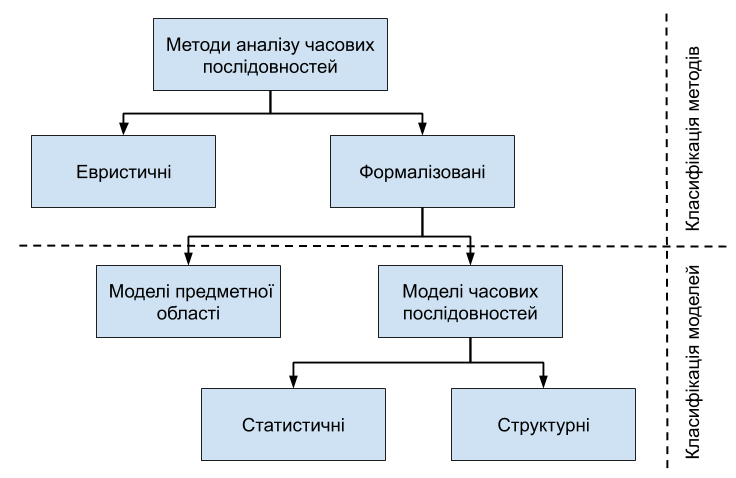
\includegraphics[scale=0.6]{method_model}
\caption{Класифікація методів та моделей аналізу часових послідовностей} 
\label{fig:method_model}
\end{center} \end{figure}

На рис.~\ref{fig:method_model} зображено класифікацію методів та моделей 
\cite{imp:Chuchueva2012}, де модель -- функціональне представлення, що з 
достатньою точністю описує досліджуваний процес, а метод являє собою 
послідовність дій які необхідно виконати для побудови моделі. Евристичні 
(інтуїтивні) методи аналізу базуються на судженнях і оцінках експертів, 
та використовуються в таких дисциплінах, як маркетинг, філософія, економіка 
і навряд підходять для виокремлення інформації з аналогового 
сигналу. Формалізовані методи дозволяють з заданою точністю побудувати 
математичну залежіть (модель), що пов'язує аналоговий сигнал та інформацію, 
що він несе. Доступні моделі розділяють на статистичні та структурні 
\cite{imp:Chuchueva2012}.

Моделі часових послідовностей базуються на методах, що шукають залежності
в середині самого нестаціонарного процесу і на цій основі виконують 
необхідний аналіз. Моделі часових послідовностей поділяються на статистичні
(регресія, EM-алгоритми, експоненційне стискання, еволюційні алгоритми, тощо)
та структурні (машинне навчання, ланцюги Маркова, класифікаційні дерева, 
узагальнене перетворення Хафа, каскади Хара, watershed, тощо). Статистичні 
моделі не придатні для застосування в розв'язанні задач виокремлення корисної 
інформації через їх алгоритмічну обчислювальну складність, натомість, 
константа складність деяких структурних алгоритмів робіть їх досить 
привабливими. Моделлю предметної області (радіофізики), у випадку виокремлення 
корисної інформації з сигналу, є послідовне застосування лінійного фільтра, 
низькошумного підсилювача, аналогово-цифрового перетворювача (АЦП) і модуля 
цифрової обробки FPGА, що переводить розв'язання в область структурної моделі
аналізу часової послідовності. В радіофізиці, такі методи застосовують як 
для задач локації \cite{imp:Dumin2017}, так і комунікації \cite{imp:Taok2009}.

Структурні моделі аналізу часових послідовностей, можна розділити за типом
інформації, що виокремлення зі вхідних даних:

\begin{enumerate}

	\item Класифікація часової послідовності (Sequence classificaion). 
	Визначення приналежності сигналу, як цілого, до певного виду (класу) 
	з наперед відомими характеристиками. Активно застосовується в задачах 
	багатопроменевої і багатокористувацької надширокосмугової комунікації. 
	Прикладом найпростішого бінарного класифікатору є визначення наявності 
	сигналу за граничним значенням (threshold value), тобто на проміжках 
	спостереження, де значення досліджуваної функції більше за наперед 
	визначене значення, бінарний класифікатор вказує True, а в інших 
	випадках False.

	\item Маркування послідовності (Sequence labeling). Визначення 
	приналежності сигналу в кожен момент часу до певного виду з наперед 
	відомими характеристиками. Активно застосовується в задачах 
	багатопроменевої і багатокористувацької надширокосмугової комунікації.

	\item Пошук аномалей (Anomaly detection). Пошук проміжку часової 
	послідовності, який вибивається з загального вигляду даних та має 
	невизначену природу. Корисний для задач, де метод максимальної 
	правдоподібності застосувати неможливо через невизначеність 
	характеристик аномалії, що шукається, наприклад задачі автоматичного 
	визначення наявності випадкових завад невідомої природи.

	\item Передбачення послідовності (Sequence forcasting). Передбачення 
	значень часової послідовності засновуватись на минулих значеннях цієї 
	послідовності. В радіофізиці активно використовуються, як моделі з 
	учителем так і без.

	\item Генерація послідовності (Sequence generation). Генерація нової 
	часової послідовності на основі наявної з урахуванням зовнішніх факторів. 
	Генерація нової послідовності може проходити, як в порядку продовження 
	або доповнення існуючої, так і в порядку створення окремої послідовності.

	\item Фільтрування послідовності (Sequence filtering). Фільтрація 
	часової послідовності від завад або сторонніх сигналів, що вона 
	містить. Спосіб визначення завад та їх ліквідація залежить від 
	імплементації конкретної моделі. Найрозповсюдженіше сімейство моделей
	фільтрації часової послідовності в радіофізиці -- лінійна фільтрація, 
	наприклад: частотні фільтри, фільтр Калмана та узгоджений фільтр.

\end{enumerate}

З іншого боку, в здачах локації, інколи застосовують методи обробки 
зображень, формуючи карти інтенсивності з отриманого сигналу. Тобто,
задача аналізу часових послідовностей зводиться до задачі комп'ютерного зору. 
Через обчислювальну складність, такі методи застосовують лише в задачах де є 
необхідність накопичувати дані і в той самий час опрацьовувати готовий пакет 
даних вже готовий пакет даних. Таким чином, до структурних моделей 
аналізу часових послідовностей можна віднести, також, і деякі моделі 
аналізу зображень:

\begin{enumerate}

	\item Класифікація зображень (Image classificaion). Визначення 
	приналежності зображення, як цілого, до певного виду (класу) з наперед 
	відомими характеристиками.

	\item Детектування об'єктів (Object detetion). Визначення положень 
	обмежувальних прямокутників для об'єктів з наперед відомими 
	характеристиками, що містяться на зображені, яке досліджується.

	\item Сегментація об'єктів (Instance segmentation). Процес розділення 
	цифрового зображення на декілька сегментів довільної форми. Під сегментом 
	мається на увазі множина пікселів, які часто називають суперпікселями. 
	Така модель сегментації не розділяє об'єкти одного типу між собою.

	\item Семантична сегментація (Semantic segmentation). Процес розділення 
	цифрового зображення на декілька сегментів довільної форми, при тому, що
	форми об'єктів одного типу семантично розділені. Найрозповсюдженішим 
	підходом до семантичного розділення об'єктів є бінарні піксельні маски. 
	Типова модель для розв'язку таких задач -- штучна згорткова нейронна 
	мережа-автоенкодер UNet.

	\item Фільтрація зображення (Image filtering). Фільтрація зображення 
	від сторонніх шумів. Зручно застосовувати для отримання обробки 
	спектральних характеристик реальних сигналів.

\end{enumerate}

Для вибору класу моделі виокремлення інформації з сигналу, а також для 
дослідження даних і імплементації моделі прийнято застосовувати  
методологію аналізу даних CRISP-DM \cite{imp:CRISPDM2000}.


%%%%%%%%%%%%%%%%%%%%%%%%%%%%%%%%%%%%%%%%%%%%%%%%%%%%%%%%%%%%%%%%%%%%%%%%%%%%%%%
\section{Структурні моделі аналізу нестаціонарних процесів}

Фізичний процес -- зміна в часі деякої фізичної величини (інколи векторної). 
В теоретичній фізиці опис процесу найчастіше являє собою безперервну часову 
послідовність, що задано математичною функцією. На практиці -- дискретну часову 
послідовність, задану масивом значень змінної в часі величини. Структурною 
моделлю аналізу процесу називатимемо формалізовану модель, що виокремлює 
з нього корисну інформацію засновуючись на закономірностях у зміні значень 
досліджуваної величини з плином часу.

Враховуючи шум в моделі інформаційного радіо-каналу \cite{imp:Shihovcev2011}, 
досліджуваний сигнал стає випадковим процесом, що ускладнює виокремлення 
корисної інформації для реальних задач. Джерелом шумів можуть бути як і 
зовнішні фактори (невідомі сторонні джерела електромагнітного поля) так і
саме обладнання прийму-передачі. Через це ускладнення базова інтуїтивна модель
виокремлення інформації, що базується на виявлені наявності сигналу за 
пороговим значенням напруженості струму стає малопридатною. Крім того,
додатковим фактором, що впливає на точність виокремлення інформації є розбіжності
протікання реального фізичного процесу передачі-поширення-прийму 
електромагнітного поля та моделі, що описує цей процес. Типовим способом 
розв'язання задач з вищезгаданими проблемами є застосування моделей з учителем
та калібрувальними параметрами.

% Прикладом такої нелінійної природи електромагнітного поля або ефектів ближньої 
% зони випромінювання призводить до спрощення моделі і викликає необхідність 
% В таких випадках застосовують методи з учителем, або калібрувальними 
% параметрами.

Основними критеріями вибору моделі стають обчислювальна складність її алгоритмів 
та точність самого методу. Для порівняння методів, а також для визначення їх 
абсолютної та відносної точності користаються широким класом метрик, але 
частіше доводиться визначати власні. Серед найчастіше вживаних метрик можна 
виокремити середню абсолютну та квадратичну помилку \cite{imp:Willmott2005}, 
але через їх недоліки часто приходять до використання більш складних методів 
оцінки точності. Недоліки таких метрик часто допомагає вирішити логарифмізація 
значення середньої помилки і деякі регуляризації отриманої функції. 
Прикладом метрики в задачах класифікації можна навести F-метрики 
\cite{imp:Tharwat2018}, а для задач сегментації та індикації використовують 
Коэффициент Жаккара (Intercection Over Union або IoU) \cite{imp:Jaccard1901}.

% декілька методів одразу

Набір моделей, які можна застосувати до часових послідовностей, значно 
розширюється, якщо застосовувати методику ковзного вікна, тобто при аналізі 
безперервної часової послідовності розглядати одномоментно деякий проміжок 
дискретних значень, що рухається в часі. Наприклад, на вхід методу лінійної 
регресії \cite{imp:Xin2009} можна подати вектор, що складається з дискретних 
послівних значень взятих з деяким інтервалом з аналогового сигналу. Якщо 
інтервал і тривалість вікна будуть вибрані правильно, то модель лінійної
регресії можливо застосувати, щоб виявити наявність імпульсу. 

З приходом ери нейронних мереж \cite{imp:Rosenblatt1957}, їх застосування в
задачах дискримінантного аналізу витісняє інші методики. Так, для більш 
складних задач, таких як класифікація імпульсу, методика ковзного вікна 
дозволяє застосовувати повнозв'язані і згорткові нейронні мережі 
\cite{imp:Plakhtii2019}.

\begin{figure}[htbp] \begin{center}
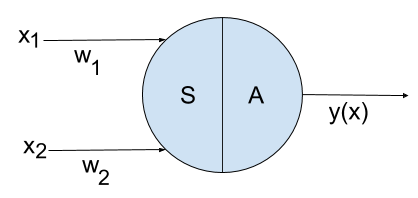
\includegraphics[scale=0.6]{perceptron}
\caption{Математична модель біологічного нейрону}
\label{fig:perceptron}
\end{center} \end{figure}

На рис.~\ref{fig:perceptron} зображено одну з математичних моделей (модель 
Розенблатта) біологічного нейрону. Вона виокремлює дві функції нейрону: 
суматору і активаційну. Біологічній нейрон розглядають, як нелінійний пристрій 
з декількома вхідними інтерфейсами (дендритами) та єдиним вихідним (аксон).
Також сам нейрон характеризується своїм внутрішнім параметрам -- зміщення 
$ b $, який відповідає за порогове значення реагування нейрону. Суматора 
функція $ S $ в моделі нейрона описує механізм акумулювання довільної 
кількості ($ n $) вхідних сигналів, поєднаних в вектор $ \vect{x} $ 
розмірністю $ n + 1 $, де останній елемент вектору завжди $ 1 $:

\begin{equation}
\func{S}{\vect{x}} = \vect{w}^\intercal \vect{x},
\end{equation}
%
де $ \vect{w}^\intercal = \left( w_1, w_2, ..., w_n, b \right) $, а
$ \vect{x} = \left( x_1, x_2, ..., x_n, 1 \right)^\intercal $.
Активаційна функція $ \func{A}{\func{S}{\vect{x}}} $ описує механізм 
реагування на акумульовані вхідні сигнали. Для класичного перцептрону 
активаційною є функція Хевісайда. Також часто застосовують сигмоїдальні 
активаційні функції та функції ReLu \cite{imp:Kussul2004}.

Разом з розповсюдженням аналогової радіоелектроніки почали заявлятись 
структурні моделі пристосовані саме для аналізу аналогових сигналів 
та часових послідовностей \cite{imp:Markov1906}. Проривом стала можливість
зберігати минулі значення послідовності у якості стану системи 
(ланцюга Маркова) і на основі цього стану проводити аналіз поточного 
значення випадкового процесу. Такий підхід дозволив скоротити кількість 
параметрів моделі у порівнянні з лінійною регресією. У порівнянні з 
багатошаровим перцептроном модель, ланцюгів Маркова показувала низьку 
запам'ятовувальну здатність, а тому в складних задачах розрізнення великої 
кількості класів показувала гірші результати.

Лише поява рекурентних нейронних мереж у 1988 році \cite{imp:Rumelhart1988} 
дозволила застосовувати на практиці моделі, що зберігають інформацію про 
випадковий процес в якості свого внутрішнього стану і не потребують 
застосування методу ковзного вікна. Цей метод та подальші його модифікації
стали перспективним напрямком розвитку структурних моделей аналізу процесів. 


%%%%%%%%%%%%%%%%%%%%%%%%%%%%%%%%%%%%%%%%%%%%%%%%%%%%%%%%%%%%%%%%%%%%%%%%%%%%%%%
\section{Рекурентні нейронні мережі тривалої короткочасної пам'яті для 
обробки нестаціонарних сигналів}

Рекурентна нейронна мережа може бути представлена, як ланцюг, що складається
з ланок (штучних нейронів), які відрізняються одна від одної лише своїм 
внутрішнім станом (рис.~\ref{fig:rnn_unrolled}). Принцип роботи цієї моделі 
засновано на типовому для радіофізики фізичному принципі зворотнього зв'язку:
вихідне значення мережі в поточний момент часу вливає на її вихідне значення 
в майбутньому.

\begin{figure}[htbp] \begin{center}
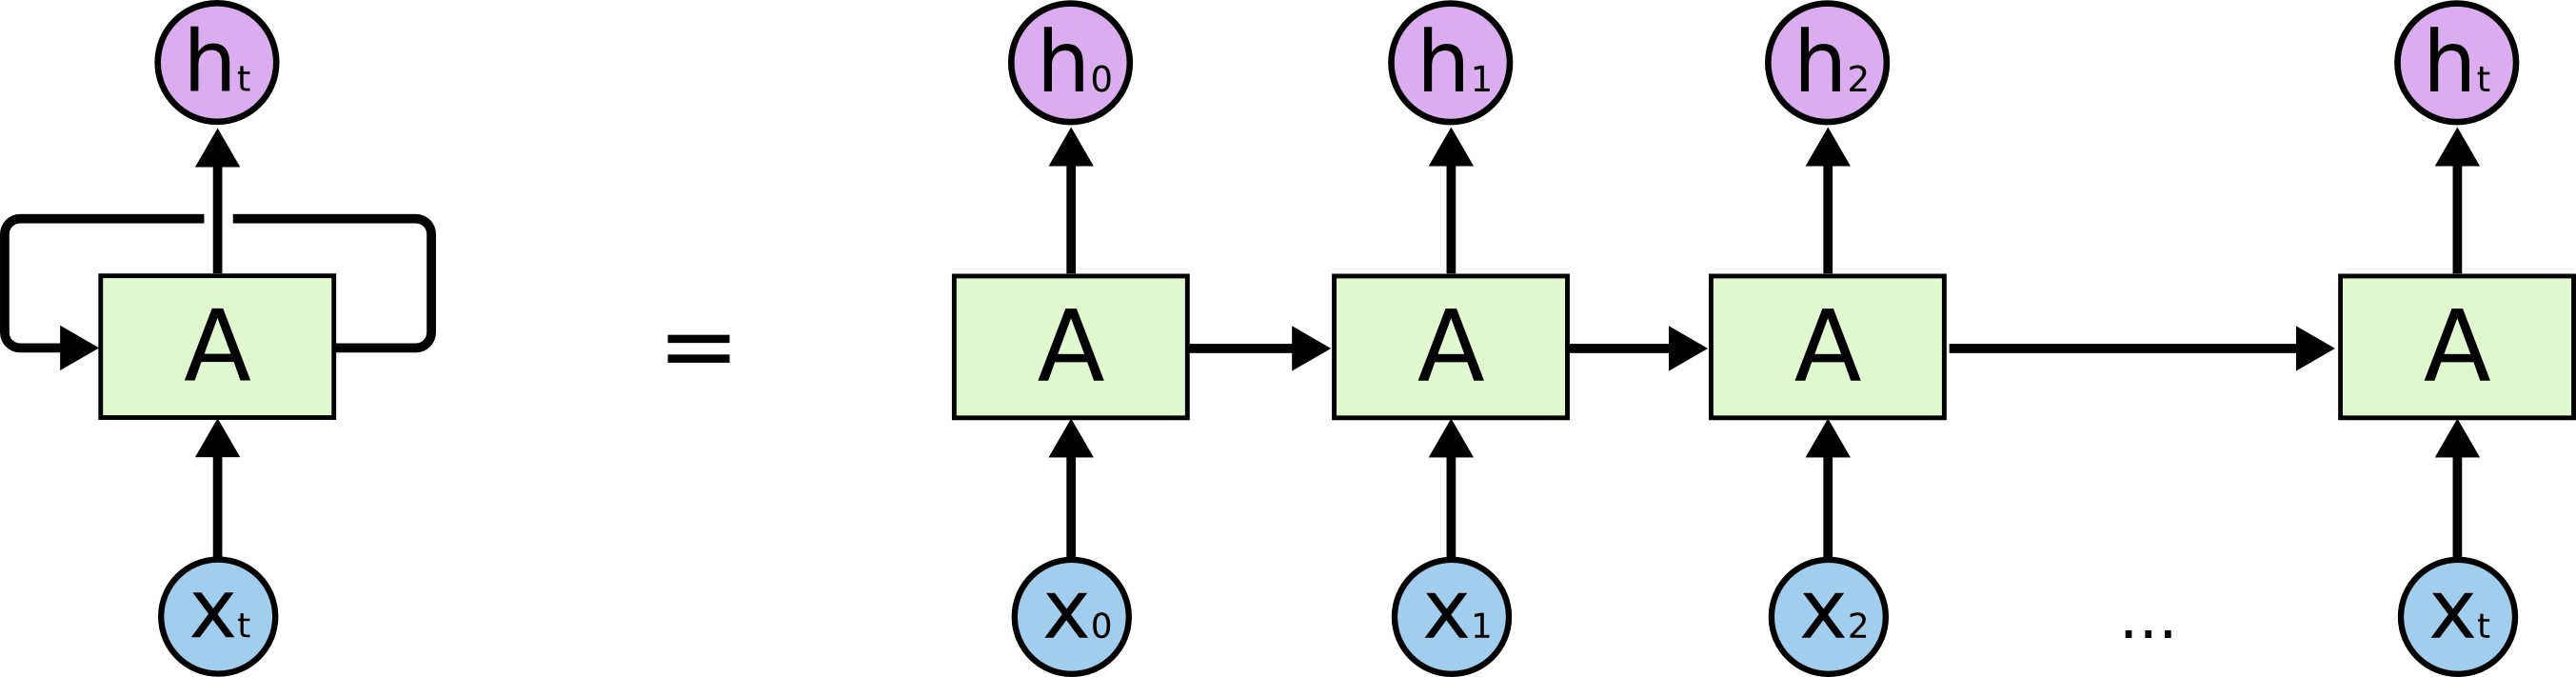
\includegraphics[scale=0.4]{rnn_unrolled}
\caption{Проходження сигналу крізь рекурентну нейронну мережу}
\label{fig:rnn_unrolled}
\end{center} \end{figure}

На рис.~\ref{fig:rnn_unrolled} літерою А позначено ланку ланцюга, $ x_i $ --
дискретне значення вхідної часової послідовності (вхід), а $ h_t $ -- якісна 
або кількісна характеристика виокремлена нейронною мережею з сигналу (вихід). 
На відміну від класичного перцептрону Розенблатта, ланки рекурентного ланцюга 
мають додатковий вихід, що передає свій внутрішній стан на наступну ланку.

Входом для такої математичної моделі є дискретизована часова послідовність 
довільної тривалості. Виходом також є часова послідовність, але не завжди з 
таким же періодом дискретизації. 

Випадок, коли частота дискретизації входу та виходу співпадає, тобто кожному 
елементу вхідної послідовності $ x_i $ підставляється окремий елемент 
вихідної $ h_i $ є найчастіше вживаним в радіофізиці. Тут кожен дискретний 
вихід моделі $ h_i $ базується на проміжку даних 
$ \left[ x_{i-j} , x_i \right] $, де $ j $ -- довільна 
кількість врахованих елементів входу, яка обмежена максимальною 
запам'ятовувальною знатністю моделі. Зазвичай, максимальна 
запам'ятовувальна знатність є гіперпараметром тренувального алгоритму 
рекурентрої мережі. Моделі такого типу відомі в закордонній літературі, як 
many-to-many.

Також зустрічаються моделі для яких частота дискретизації входу та виходу 
не співпадає. В моделях де одному вхідному дискретному значенню 
співставляєтья деякий проміжок вихідної послідовності називають one-to-many.
Прикладом one-to-many задачі є підвищення якості звуку. Задачі, в яких 
навпаки, деякому проміжку вхідних значень $ \left[ x_{i-N} , x_i \right] $, 
де $ N $ -- стала константа, співставляється одне вихідне значення $ h_i $
називають many-to-one. На відміну від many-to-many задач, тут 
дискретне вихідне значення базується на проміжку вхідних даних сталої 
тривалості, що накладає деякі обмеження на застосування моделі. Такий 
підхід еквівалентний застосуванню методики ковзного вікна.

Підхід із застосуванням медики ковзного вікна має суттєвий недолік: 
тривалість вікна залишається сталою, коли тривалість сигналу залежить від 
багатьох факторів, а отже вибирати тривалість вікна треба з огляду на 
максимально можливу тривалість імпульсу. Це призводить до того, що для 
більш коротких імпульсів модель може втратити точність. В задачах локації, 
де корисна інформація знаходиться в післяімпульсних коливаннях, тривалість 
яких взагалі не обмежена, застосування методики ковзного вікна принципово 
неможливе без обмеження на глибину зондування.

Сьогодні, прижились дві реалізації ланок рекурентних мереж, які застосовують,
як для many-to-one так і для many-to-many -- це LSTM та GRU, які дуже схожі 
за своїми можливостями. Класичні RNN без механізму забування вважаються менш 
ефективними через низьку максимальну запам'ятовувальну знатність.

\begin{figure}[htbp] \begin{center}
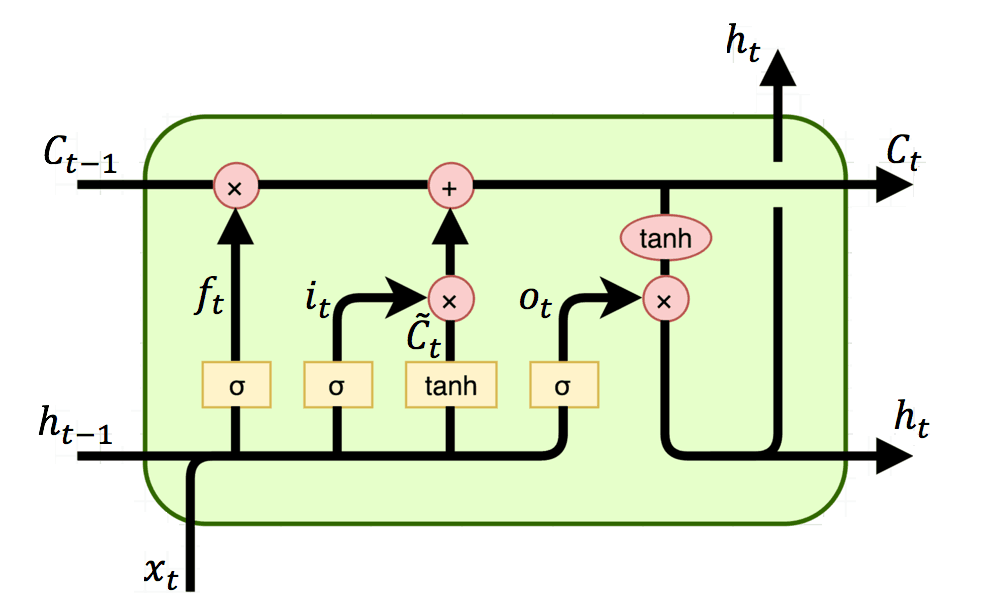
\includegraphics[scale=0.5]{lstm_inside}
\caption{Внутрішня структура ланки ланцюга LSTM}
\label{fig:lstm_inside}
\end{center} \end{figure}

На рис.~\ref{fig:lstm_inside} з \cite{imp:Varsamopoulos2018} зображено 
внутрішню будову ланки рекурентної мережі довготривалої та короткотривалої 
пам'яті. Символом множення на рисунку позначена операція множення чисел, а 
плюсом -- додавання. Також, жовтими прямокутниками позначено функції, що діють 
на число: $ \tanh $ -- гіперболічний тангенс та $ \sigma $ -- сигмоїда.

Передача внутрішнього стану $ C_t $ на наступну ланку здійснюється по 
верхній горизонтальній стрілці, де цей внутрішній стан змінюється на основі
поточного значення вхідної часової послідовності $ x_t $ та передбачення 
моделі на минулій ланці $ h_{t-1} $.

Першим етапом обробки часової послідовності є так званий поріг забування
(або forget gate). При проходженні крізь нього ми визначаємо яку 
кількість інформації про часову послідовність слід забути:

\begin{equation}
f_t = \func{\sigma}{\dotprod{W_f}{\crossprod{h_{t-1}}{x_t}} + b_f},
\end{equation}
%
де $ W_f $ і $ b_f $ -- матричні тренувальні параметри.

Наступний етап визначає на скільки потенційно важливим може стати поточне 
значення нейронної мережі та чи треба зберігати його у внутрішньому стані. 
Цей етап називають прохідний поріг (або input gate):

\begin{equation}
i_t = \func{\sigma}{\dotprod{W_i}{\crossprod{h_{t-1}}{x_t}} + b_i},
\end{equation}

\begin{equation}
\tilde{C_t} = \func{\tanh}{\dotprod{W_C}{\crossprod{h_{t-1}}{x_t}} + b_C},
\end{equation}
%
де $ W_C, b_C $ -- матричні тренувальні параметри.

Користуючись отриманими значеннями прохідного порогу і порогу забування
можна змінити внутрішній стан моделі:

\begin{equation}
C_t = f_t C_{t-1} + i_t \tilde{C_t}.
\end{equation}

Отримавши новий внутрішній стан моделі $ C_t $ можна отримати поточне вихідне 
значення (передбачення) $ h_t $ користуючись поточним вхідним значенням 
$ x_t $ послідовності, як порогом забування:

\begin{equation}
o_t = \func{\sigma}{\dotprod{W_o}{\crossprod{h_{t-1}}{x_t}} + b_o},
\end{equation}

\begin{equation}
h_t = o_t \func{\tanh}{C_t},
\end{equation}
%
де $ W_o, b_o $ -- матричні тренувальні параметри.

Алгоритмом зворотнього поширення помилки знаходять тренувальні 
параметри $ W_f, b_f, W_C, b_C, W_o, b_o $. На відміну від повнозв'язних ШНМ, 
алгоритм зворотнього поширення помилки повинен враховувати не лише пари даних 
входу та виходу моделі, а ще проміжний результат у вигляді зміни внутрішнього 
стану нейронної мережі $ \partder{C_t}{x_t} $.

\chapter{Імпульсне поле випромінювача з круговою апертурою}
\label{ch:linear}

%%%%%%%%%%%%%%%%%%%%%%%%%%%%%%%%%%%%%%%%%%%%%%%%%%%%%%%%%%%%%%%%%%%%%%%%%%%%%%%
\section{Кругова апертура як модель антен імпульсного випромінювання}

На початку 60-х років інтерес до імпульсної радіофізики був збуджений
військовим застосуванням переваг надширокосмугових радарних та 
телекомунікаційних систем. Дослідження велись, як в Україні 
\cite{imp:Dumin1996} так і за кордоном \cite{imp:BaumIN0105}. Ці дослідження, сьогодні,
знайшли своє застосування у системах інтернету речей \cite{imp:Hartmann2015}, 
автомобільної індустрії \cite{imp:Yarovoy2017}, а також медицині 
\cite{imp:Cho2016}.

Широким класом технічних рішень для формування напрямленого випромінювання 
надширокосмугового електричного струму є антени імпульсного випромінювання.
Такі антени можна класифікувати за способом вирівнювання фронту хвиль:

\begin{enumerate}
	\item без вирівнювання сферичного фронту;
	\item лінзові сповільнювачі;
	\item рефлекторні антени;
	\item комбіновані архітектури \cite{imp:BaumSSN0379}.
\end{enumerate}

Живлення для таких антен зазвичай виконується ТЕМ рупором, що під'єднується 
до коаксіального кабелю через балун \cite{imp:BaumSSN0357}. Даний розділ 
присвячується дослідженню саме лінзових антен імпульсного випромінювання (LIRA). 

Антени типу LIRA мають численні переваги над рефлекторними. Перш за все, це
більш високий коефіцієнт підсилення антени \cite{imp:BaumUWBSP1}. По-друге,
лінзові антени не мають області тіні від опромінювача та краще узгоджуються
на практиці \cite{imp:BaumSSN0377}. Також експериментальне порівняння LIRA 
з рефлекторними антенами показує, що імпульсні характеристики перших мають 
меншу тривалість при тих самих електричного розмірах \cite{imp:BaumSSN0377}.
З недоліків варто відзначити важкість виготовлення лінз точної форми та 
вагу антени.

Розглянемо задачу збудження такої антени нестаціонарним імпульсним струмом
з деякою часовою залежністю $ f(t) $ з умовою існування першої та другої 
похідної для $ f(t) $. Ефективна тривалість перехідного процесу $ f(t) $ 
прийнято визначати за повною шириною на рівні половинної амплітуди 
(full width at half maximum або FWHM), що зручно на практиці. 
В роботі діапазон значень ефективної тривалості розглядається в межах 
від десятків пікосекунд до декількох наносекунд, що є найбільш цікавим 
діапазоном тривалостей для сучасної надширокосмугової електроніки.

Сферична хвиля проходить крізь систему діелектричних лінз, розташованих у 
розкриві, формуючи квазі-одномоментне збудження плаского фронту у розкриві. 
Формою розкриву, зазвичай, вибирають кругову апертуру. Таким чином, у першому 
наближенні, у розкриві формується рівномірно розподілений сторонній плаский 
електричний струм, напрямлений від одного плеча рупора до іншого. Вперше така
апроксимація була запропонована 1985 р. \cite{imp:Wu1985} та 
емпірично перевірена через декілька років \cite{imp:Wu1991}.

Серед лінзового класу антен, що формують розподіл стороннього струму у 
вигляді плаского диску варто відзначити антену Рис.~\ref{fig:lira_baum}, що 
спершу представив Ву \cite{imp:Wu1987}, а згодом і, незалежно, Карл Баум 
\cite{imp:BaumSSN0377}. Лінза антени виконана у формі витягнутого сфероїда, 
а розкрив ТЕМ-рупора цілком заповнено діелектриком. Повне заповнення 
розкриву рупора мінімізує відбиття та покращує стійкість антени до механічних 
пошкоджень \cite{imp:BaumSSN0377}. Скруглений рупор починається в одному 
фокусі еліпсоїда, а закінчується в другому, таким чином радіус розкриву є 
фокальним параметром еліпсоїда. В якості матеріалу для лінзи пропонується 
використовувати поліетилен високої густини (HDPE) з низькою діелектричною 
проникністю $\epsilon = 2.3 $.

\begin{figure}[htbp] \begin{center}
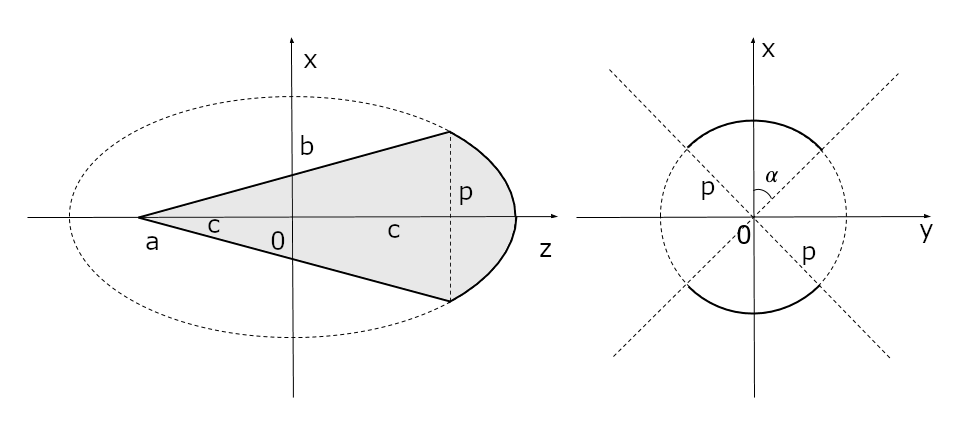
\includegraphics[scale=0.5]{Baum_LIRA}
\caption{Геометрія лінзевої антени Баума та Ву} \label{fig:lira_baum}
\end{center} \end{figure}

При використанні апроксимації плаского диску з електричним струмом для 
розв'язання задачі випромінювання антени зі сфероїдоподібною лінзою 
помічаємо, що уявний диск зі струмом і поверхня рівних фаз будуть розташовані 
поза межами розкриву рупора. Як покажемо далі, це не впливає на точність 
моделі, як в ближній, так і в дальній зоні, а відхилення тримаються в межах
систематичної похибки через внутрішній опір антени, який модель не враховує.

В 1991 р. Ву представив антену, для якої уявний диск зі струмом буде 
розташовуватись у розкриві рупора \cite{imp:Wu1991}. Гіперболічна лінза в 
цій антені забезпечує положення поверхні рівних фаз в самому розкриві 
Рис. \ref{fig:lira_wu}. Одним з способів покращити цю антену є 
заміна діелектричного наповнення $ \epsilon_1 $ та лінзи $ \epsilon_2 $ на 
матеріал, діелектрична характеристика якого є функцією координат 
$ \epsilon(\rho, z) $. Таким чином, відбиття від внутрішньої поверхні лінзи 
знижується і характеристики антени покращуються. Важливим мінусом такої 
конструкції стає важкість виготовлення лінзи.

\begin{figure}[htbp] \begin{center}
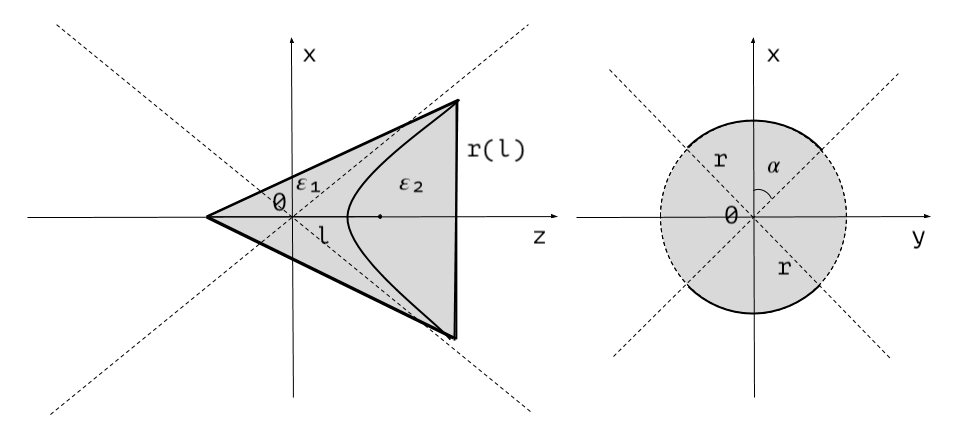
\includegraphics[scale=0.5]{Wu_LIRA}
\caption{Геометрія лінзової антени Ву} \label{fig:lira_wu}
\end{center} \end{figure}

\vspace{8mm}
Призначенням LIRA є телекомунікація, радіолокація і лабораторні вимірювання. 
Проте, цікавість таких антен пояснюється ще і аномально повільним згасанням 
енергії імпульсного поля з відстанню, що було теоретично передбачено 
\cite{imp:Wu1987}. Цей ефект відомий у вітчизняній та закордонній літературі 
за назвою електромагнітний снаряд (electromagnetic missile).

Фізична модель плаского диску описує поле LIRA лише у першому наближенні.
Така модель не враховує вихровий магнітний сторонній струм, що існує на ряду 
з пласким електричним, а також не враховує струми, що течуть назад в 
генератор відбившись від краю рупора - поле такого струму залишає ``хвіст'' 
після основного імпульсу. Проте, емпіричні дослідження 
\cite{imp:BaumSSN0396,imp:BaumSSN0401} показують, що при належному 
узгодженні, паразитний вплив відбиття фактично відсутній, а перехідна 
функція отримана експериментальним шляхом і відповідає моделі плаского диску.

Для отримання розв'язку задачі плаского диску застосовували широкий спектр 
методів. Першими були отримані наближені розв'язки в частотній області 
\cite{imp:Wu1985,imp:Sodin1992-10}. Також, розв'язок для цієї задачі частково
знайдено у часовій області \cite{imp:Dumin1996}. Недоліком наявних розв'язків 
є те, що вони не надають часову залежність напруженості поля в довільних точках 
спостереження в явному виді, а отже не можуть використовуватись в широкому 
спектрі практичних задач, як, наприклад, врахування ефектів самодії у 
нелінійному середовищі. При самоїді поля крізь середовище, на значення 
напруженості поля в кожній точці спостереження та в будь-який момент часу 
впливають всі причинно пов'язані зі спостереженням події. Таким чином, 
наявність розв'язання в будь-якій точці спостереження - необхідна умова для 
врахування нелінійних ефектів методом теорії збурень.

\begin{figure}[htbp] \begin{center}
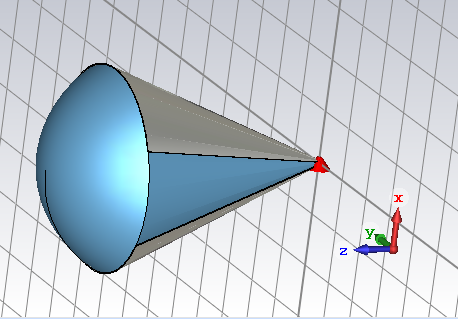
\includegraphics[scale=1.35]{lira_cst}
\caption{Модель антени в симуляторі CST Studio} \label{fig:lira_cst}
\end{center} \end{figure}

%%%%%%%%%%%%%%%%%%%%%%%%%%%%%%%%%%%%%%%%%%%%%%%%%%%%%%%%%%%%%%%%%%%%%%%%%%%%%%%
\section{Розв'язання методом еволюційних рівнянь} \label{sec:tranc_resp}

Розглянемо сторонній електричний нестаціонарний струм $ \vect{j_0} (r,t) $ 
в якості єдиного джерела електромагнітного поля. Нехай струм 
однонапрямлений, рівномірнорозподілений та має форму плаского диску 
нульової товщини. Для розв'язання прямої задачі електродинаміки для 
довільної часової залежності $ f(t) $ нестаціонарного струму 
$ \vect{j_0} (r,t) $ достатньо отримати розв'язок для  $ f(t) = H(t) $, 
де $ H(t) $ - функція Хевісайда, а далі, користуючись принципом суперпозиції
будувати розв'язок для довільної часової залежності $ f(t) $.
Тоді, джерело, що розглядається, математично можна описати в циліндричних 
координатах $ \rho, \varphi, z $, як

\begin{equation}
\vect{j_0} \left( r, t \right) = \vect{J} = \vect{x_0} A_0 H(t) \delta(z) 
\left(  H(\rho) - H(\rho - R) \right),
\end{equation}
%
де $ A_0 $ - максимальна амплітуда струму, що вимірюється в В/м, $ R $ - 
радіус диску, що вимірюється в метрах, $ \delta(z) $ - символ Кронекера, а 
$ \vect{x_0} = \vect{\rho_0} \cos \varphi - \vect{\varphi_0} \sin \varphi $ 
- декартовий орт OX, як показано на Рис.~\ref{fig:pdisk}.

\begin{figure}[htbp] \begin{center}
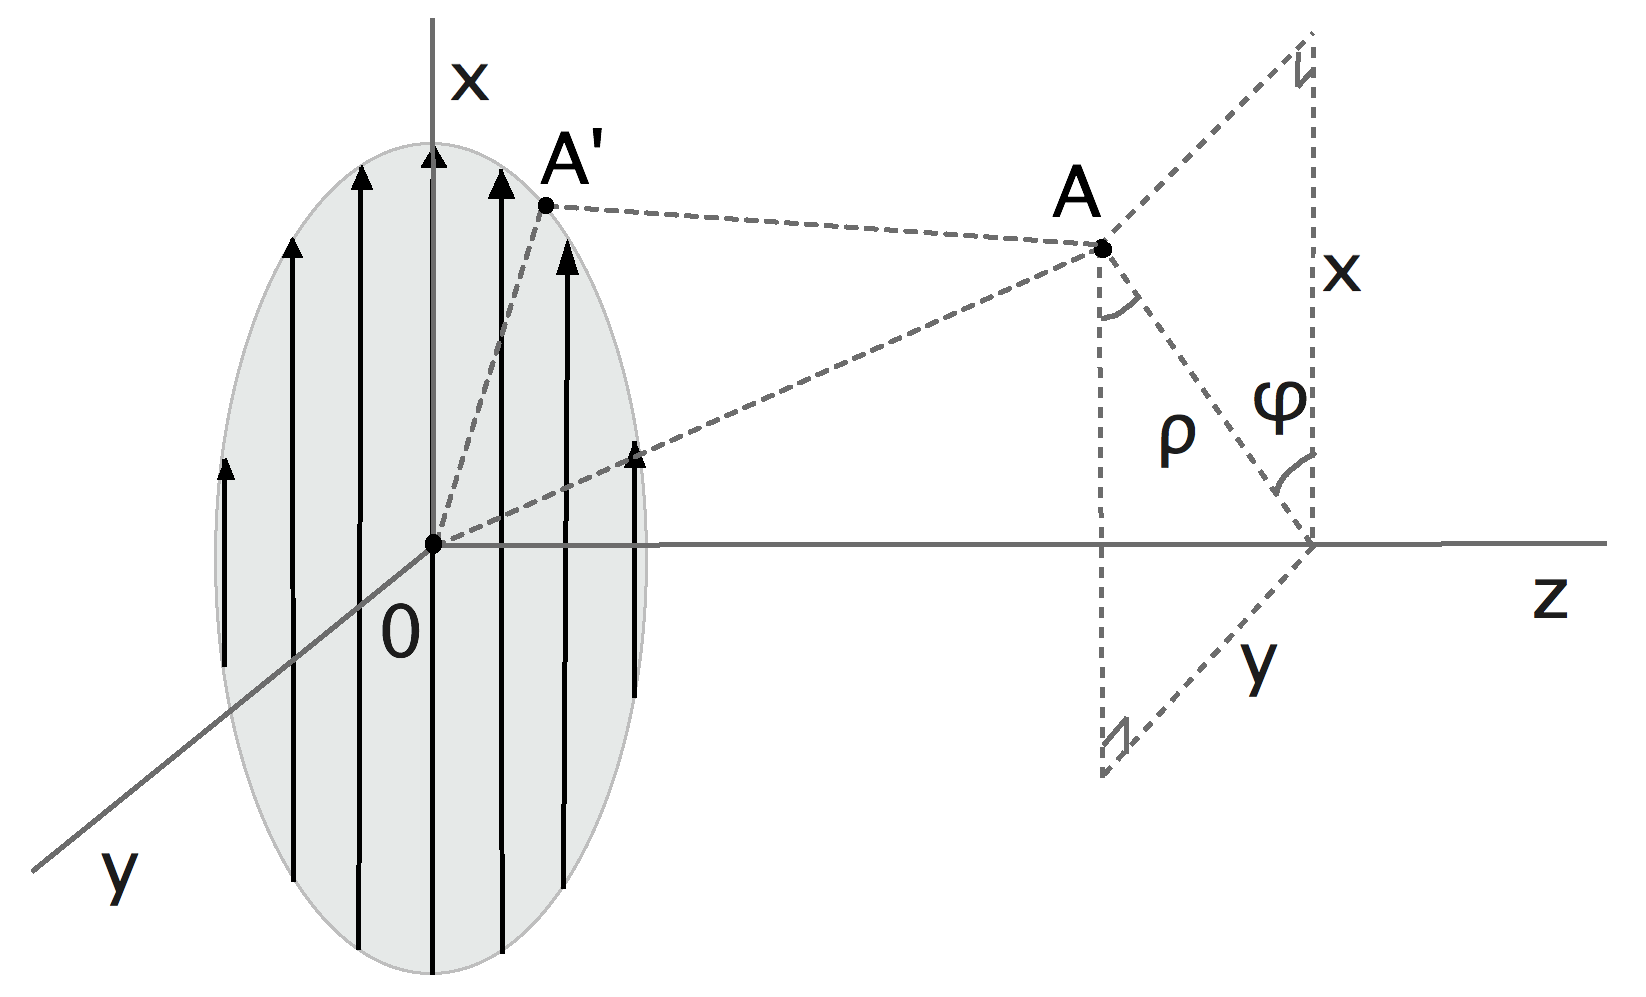
\includegraphics[scale=0.55]{PlaneDisk}
\caption{Геометрія випромінювача} \label{fig:pdisk}
\end{center} \end{figure}
%
%\textcolor{blue} { \begin{equation*} \begin{aligned}
%\begin{cases}
%\vect{\rho_0} = \vect{x_0} \cos \varphi + \vect{y_0} \sin \varphi \\
%\vect{\varphi_0} = - \vect{x_0} \sin \varphi + \vect{y_0} \cos \varphi
%\end{cases} \Rightarrow \mathbf{A} = \left( \begin{array}{cc}
%\cos \varphi & \sin \varphi \\
%- \sin \varphi & \cos \varphi
%\end{array} \right)
%\end{aligned} \end{equation*} }
%
%\textcolor{blue} { \begin{equation*} \begin{aligned}
%\vect{j_0} \left( \vect{\rho_0}, \vect{\varphi_0} \right) = 
%\mathbf{A} \vect{j_0} \left( \vect{x_0}, \vect{y_0} \right) = \\
%= H(t) \delta(z) (  H(\rho) - H(\rho - R) ) 
%( \vect{\rho_0} \cos \varphi - \vect{\varphi_0} \sin \varphi )
%\end{aligned} \end{equation*} }
%
Для застосування методу еволюційних рівнянь, спершу, знайдемо модовий 
розклад струму, застосувавши наступне перетворення

\begin{equation} \label{eq:jm_base}
j_m \left( r, t; \nu \right) = \frac{\sqrt{\mu_0}}{2\pi} 
\int \limits_{0}^{2\pi} d \varphi \int \limits_{0}^{\infty} \rho d \rho 
\vect{j_0} \crossprod{ \nabla_\perp \Psi_m^* }{ \vect{z_0} },
\end{equation}
%
де $ \Psi_m^* $ - комплексно спряжена базисна функція \cite{imp:Dumin2010}.
%
%\textcolor{blue} { \begin{equation*} \begin{aligned}
%\crossprod{ \nabla_\perp \Psi_m^* }{ \vect{z_0} } = 
%- \sqrt{\nu} e^{-im\varphi} \left( 
%\vect{\varphi_0} \frac{J_{m-1} (\nu \rho) - J_{m+1} (\nu \rho)}{2} + 
%\right. \\ + \left. i m \vect{\rho_0} \frac{J_m (\nu \rho)}
%{\rho \nu} \right) = - \sqrt{\nu} e^{-im\varphi} \left( 
%\vect{\varphi_0} \frac{J_{m-1} (\nu \rho) - J_{m+1} (\nu \rho)}{2} + 
%\right. \\ + \left. i \vect{\rho_0} \frac{J_{m-1} (\nu \rho) + 
%J_{m+1} (\nu \rho)}{2} \right)
%\end{aligned} \end{equation*} }
%
%\textcolor{blue} { \begin{equation*} \begin{aligned}
%\vect{j_0} \crossprod{ \nabla_\perp \Psi_m^* }{ \vect{z_0} } = 
%- \sqrt{\nu} ( \cos m \varphi - i \sin m \varphi ) 
%H(t) \delta(z) ( H(\rho) - H(\rho - R) ) \cdot \\ \cdot \left( 
%i \frac{J_{m-1} (\nu \rho) + J_{m+1} (\nu \rho)}{2} \cos \varphi
%- \frac{J_{m-1} (\nu \rho) - J_{m+1} (\nu \rho)}{2} \sin \varphi
%\right)
%\end{aligned} \end{equation*} }
%
%\textcolor{blue} { \begin{equation*} \begin{aligned}
%j_m = \frac{\sqrt{\mu_0}}{2\pi} \sqrt{\nu} \delta(z) H(t) \cdot \\
%\cdot \Big( \int \limits_{0}^{2\pi} d \varphi \sin \varphi 
%( \cos m \varphi - i \sin m \varphi) \int \limits_{0}^{R} 
%\frac{J_{m-1} (\nu \rho) - J_{m+1} (\nu \rho)}{2} \rho d \rho - \\
%- i \int \limits_{0}^{2\pi} d \varphi \cos \varphi 
%( \cos m \varphi - i \sin m \varphi) \int \limits_{0}^{R} 
%\frac{J_{m-1} (\nu \rho) + J_{m+1} (\nu \rho)}{2} \rho d \rho \Big)
%\end{aligned} \end{equation*} }
%
%\textcolor{blue} { \begin{equation*} \begin{aligned}
%j_m = \frac{\sqrt{\mu_0}}{2\pi} \sqrt{\nu} \delta(z) H(t) 
%i\pi ( \delta_{m,-1} - \delta_{m,1} ) \int \limits_{0}^{R} 
%\frac{J_{m-1} (\nu \rho) - J_{m+1} (\nu \rho)}{2} \rho d \rho - \\
%- \frac{\sqrt{\mu_0}}{2\pi} \sqrt{\nu} \delta(z) H(t) 
%i\pi ( \delta_{m,-1} + \delta_{m,1} ) \int \limits_{0}^{R} 
%\frac{J_{m-1} (\nu \rho) + J_{m+1} (\nu \rho)}{2} \rho d \rho =
%\end{aligned} \end{equation*} }
%
%\textcolor{blue} { \begin{equation*} \begin{aligned}
%= i \frac{\sqrt{\mu_0 \nu}}{4} \delta(z) H(t)
%\delta_{m,-1} \int \limits_{0}^{R} \left( J_{-2} (\nu \rho) - 
%J_0 (\nu \rho) \right) \rho d \rho - \\
%- i \frac{\sqrt{\mu_0 \nu}}{4} \delta(z) H(t)
%\delta_{m,1} \int \limits_{0}^{R} \left( J_{0} (\nu \rho) - 
%J_2 (\nu \rho) \right) \rho d \rho - \\
%- i \frac{\sqrt{\mu_0 \nu}}{4} \delta(z) H(t)
%\delta_{m,-1} \int \limits_{0}^{R} \left( J_{-2} (\nu \rho) +  
%J_0 (\nu \rho) \right) \rho d \rho - \\
%- i \frac{\sqrt{\mu_0 \nu}}{4} \delta(z) H(t)
%\delta_{m,1} \int \limits_{0}^{R} \left( J_{0} (\nu \rho) +
%J_2 (\nu \rho) \right) \rho d \rho =
%\end{aligned} \end{equation*} }
%
%\textcolor{blue} { \begin{equation*} \begin{aligned}
%= - i \frac{\sqrt{\mu_0 \nu}}{2} \delta(z) H(t) 
%(\delta_{m,1} + \delta_{m,-1}) 
%\int \limits_{0}^{R} \left( J_{0} (\nu \rho) + 
%J_2 (\nu \rho) \right) \rho d \rho - \\
%- i \frac{\sqrt{\mu_0 \nu}}{2} \delta(z) H(t) 
%(\delta_{m,1} + \delta_{m,-1}) 
%\int \limits_{0}^{R} \left( J_{0} (\nu \rho) -
%J_2 (\nu \rho) \right) \rho d \rho = \\
%= - i \frac{\sqrt{\mu_0 \nu}}{2} \delta(z) H(t) 
%(\delta_{m,1} + \delta_{m,-1}) 
%\int \limits_{0}^{R} J_{0} (\nu \rho) \rho d \rho
%\end{aligned} \end{equation*} }
%
%\textcolor{blue} { \begin{equation*} \begin{aligned}
%\int \limits_{0}^{R} J_{0} (\nu \rho) \rho d \rho = 
%\frac{1}{\nu^2} \int \limits_{0}^{R} J_{0} (\nu \rho) \nu \rho d \nu \rho =
%\left. \frac{\rho J_1 (\nu \rho) }{\nu} \right|_{0}^{R} = 
%\frac{R J_1 (\nu R)}{\nu}
%\end{aligned} \end{equation*} }
%
Після інтегрування $ \eqref{eq:jm_base} $ за кутом $ \varphi $ отримаємо 
тільки дві не нульові рівні між собою моди, які зручно записати одним 
виразом, використовуючи символи Кронекера $ \delta_{m,\pm1} $:

\begin{equation} 
j_m (z, t; \nu) = - i R A_0 \frac{\sqrt{\mu_0}}{2} \delta(z) H(t) 
\frac{\delta_{m,1} + \delta_{m,-1}}{\sqrt{\nu}} J_1 (\nu R).
\end{equation}

У методі еволюційних рівнянь електромагнітне поле є розкладом за 
деякими базисними функціями. Для ТЕ задач випромінювання, як ця, еволюційні 
рівняння значно спрощуються, а самі коефіцієнти стають пропорційними.
Фактично, пошук еволюційних коефіцієнтів зводиться до розв'язання одного
рівняння Клейна-Гордона відносно $ h_1 $ та $ h_{-1} $
%
%\textcolor{blue} { \begin{equation*} \begin{aligned}
%- \epsilon \partial_{ct} (V_m^h) - \partial_z I_m^h + \nu^2 h_m = 
%\frac{\sqrt{\mu_0}}{2 \pi} \int_0^{2\pi} d \varphi 
%\int_0^{\infty} \rho d \rho \crossprod{\vect{z_0}}{\vect{J_\perp}}
%\nabla_\perp \Psi_m^* (\nu) 
%\end{aligned} \end{equation*} }
%
%\textcolor{blue} { \begin{equation*} \begin{aligned}
%\crossprod{\vect{z_0}}{\vect{J_\perp}} \nabla_\perp \Psi_m^* (\nu) =
%\vect{J_\perp} \crossprod{\nabla_\perp \Psi_m^* (\nu)}{\vect{z_0}}
%\end{aligned} \end{equation*} }
%
%\textcolor{blue} { \begin{equation*} \begin{aligned}
%\epsilon \partial_{ct} \left( \mu \partial_{ct} h_m \right) -
%\mu^{-1} \partial_z \left( \mu  \partial_z h_m \right) + 
%\nu^2 h_m = j_m (z,t,\nu)
%\end{aligned} \end{equation*} }
%
\begin{equation} \begin{aligned} \label{eq:klein_gordon}
\frac{\epsilon \mu}{c^2} \frac{\partial^2 h_m}{\partial t^2} - 
\frac{\partial^2 h_m}{\partial z^2} + \nu^2 h_m = j_m (z,t,\nu).
\end{aligned} \end{equation}
%
Рівняння \eqref{eq:klein_gordon} було отримано з припущенням, що середовище 
в якому поширюється поле однорідне, стаціонарне та характеризується 
відносною діелектричною $ \epsilon $ та магнітною $ \mu $ проникненнями.
Буде зручно позначити швидкість світла в цьому середовищі за 
$ v = \frac{c}{\sqrt{\epsilon \mu}} $. Рівняння Клейна-Гордона
має відомий розв'язок через функцію Рімана:

\begin{equation} \label{eq:klein_gordon_sol}
h_m (z, t; \nu) = \iint_S j_m (t',z') G(t,t',z,z') dt' dz',
\end{equation}
%
де $ G(t,t',z,z') $ функція Рімана 
%
%\begin{equation*}
%G = \frac{\mathit{v}}{2} H \left( \mathit{v} (t-t') - (z-z') \right)
%J_0 \left( \nu \sqrt{\mathit{v}^2 (t-t')^2 - (z-z')^2} \right).
%\end{equation*}
%
З вигляду розв'язку \eqref{eq:klein_gordon_sol} можна зробити висновок, що
функція Рімана $ G(t,t',z,z') $ - це аналог функції Гріна в часовому просторі,
а розв'язок рівняння Клейна-Гордона є еквівалентом принципу суперпозиції
для сферичних нестаціонарних хвиль, що випромінюються кожною з точок джерела
(випромінювачами Гюгенца) у деякій точці спостереження у визначений час.
%
%\textcolor{blue} { \begin{equation*} \begin{aligned}
%h_m (z, t; \nu) = - i \mathit{V} R \frac{\sqrt{\mu_0}}{4} 
%\frac{\delta_{m,1} + \delta_{m,-1}}{\sqrt{\nu}} J_1 (\nu R)
%\int \limits_{0}^{\infty} \delta(z) \cdot \\ \cdot
%\int \limits_{t - \frac{z}{\mathit{V}}}^{0} 
%J_0 \left( \nu \sqrt{\mathit{V}^2 (t-t')^2 - (z-z')^2} \right) dt' dz' = 
%i \mathit{V} R \frac{\sqrt{\mu_0}}{4} 
%\frac{\delta_{m,1} + \delta_{m,-1}}{\sqrt{\nu}} J_1 (\nu R)
%\cdot \\ \cdot \int \limits_{0}^{\infty} \delta(z)
%\int \limits_{0}^{t - \frac{z}{\mathit{V}}} 
%J_0 \left( \nu \sqrt{\mathit{V}^2 (t-t')^2 - (z-z')^2} \right) dt' dz
%\end{aligned} \end{equation*} }
%
%\textcolor{blue} { \begin{equation*} \begin{aligned}
%h_m (z, t; \nu) = i \mathit{V} R \frac{\sqrt{\mu_0}}{4} 
%\frac{\delta_{m,1} + \delta_{m,-1}}{\sqrt{\nu}} J_1 (\nu R)
%\int \limits_{0}^{t - \frac{z}{\mathit{V}}} 
%J_0 \left( \nu \sqrt{\mathit{V}^2 (t-t')^2 - z^2} \right) dt'
%\end{aligned} \end{equation*} }
%
Користуючись властивостями дельта-функції Дірака та функції Хевісайда 
запишемо поздовжні модові коефіцієнти $ h_1 $ та $ h_{-1} $ в наступному 
виді:

\begin{equation} \label{eq:hm_int}
h_m = \frac{i R A_0}{4} \frac{\delta_{m,1} + \delta_{m,-1}}
{\sqrt{\nu} \sqrt{\epsilon_0 \epsilon \mu}} J_1 (\nu R) 
\int \limits_{0}^{t - \frac{z}{v}} 
J_0 \left( \nu \sqrt{v^2 (t-t')^2 - z^2} \right) dt'.
\end{equation}

Знайшовши поздовжній магнітний модовий коефіцієнт, 
поперечні морові коефіцієнти нескладно визначити через нього. 
Для отримання виразу для $ V_m^h = - \frac{\mu}{c} \partder{h_m}{t} $
необов'язково брати інтеграл в $ h_m $. Спробуємо спростити 
вираз, скориставшись залежністю через похідну по часу, тобто 
застосуємо правило інтегрування Лейбніца \cite{imp:Flanders1973}, 
помітивши, що

\begin{equation*} \begin{aligned}
\partder{}{t'} J_0 \left( \nu \sqrt{v^2 (t-t')^2 - z} \right) =
- \partder{}{t} J_0 \left( \nu \sqrt{v^2 (t-t')^2 - z} \right).
\end{aligned} \end{equation*}

%
%\textcolor{blue} { \begin{equation*} \begin{aligned}
%\partder{}{\theta} \int_{a(\theta)}^{b(\theta)} f(x,\theta) dx = 
%\int_{a(\theta)}^{b(\theta)} \partder{f}{\theta} dx + 
%f\big( b(\theta), \theta \big) \partder{b}{\theta} -
%f\big( a(\theta), \theta \big) \partder{a}{\theta}
%\end{aligned} \end{equation*} }
%
%\textcolor{blue} { \begin{equation*} \begin{aligned}
%\partder{}{t} J_0 \left( \nu \sqrt{v^2 (t-t')^2 - z} \right) = 
%- \nu J_1 \left( \nu \sqrt{v^2 (t-t')^2 - z} \right) 
%\partder{}{t} \sqrt{v^2 (t-t')^2 - z} = \\
%-  J_1 \left( \nu \sqrt{v^2 (t-t')^2 - z} \right)
%\frac{2 \nu v^2 (t-t')}{2 \sqrt{v^2 (t-t')^2 - z}} = - \nu v^2 (t-t') 
%\frac{J_1 \left( \nu \sqrt{v^2 (t-t')^2 - z} \right)}
%     {\sqrt{v^2 (t-t')^2 - z}}
%\end{aligned} \end{equation*} }
%
%\textcolor{blue} { \begin{equation*} \begin{aligned}
%\partder{}{t} \int \limits_{0}^{t - \frac{z}{v}} 
%J_0 \left( \nu \sqrt{v^2 (t-t')^2 - z^2} \right) dt' = \\
%= \int \limits_{0}^{t - \frac{z}{v}} 
%\partder{}{t} J_0 \left( \nu \sqrt{v^2 (t-t')^2 - z^2} \right) dt' +
%J_0 (0) - 0 \cdot \left( \nu \sqrt{v^2 (t-t')^2 - z^2} \right) = \\
%= - \int \limits_{0}^{t - \frac{z}{v}} 
%\partder{}{t'} J_0 \left( \nu \sqrt{v^2 (t-t')^2 - z^2} \right) dt' + 1 =
%- \Big. J_0 \left( \nu \sqrt{v^2 (t-t')^2 - z^2} \right) \Big|_{0}^{t - \frac{z}{v}} + 1 = \\
%- J_0 \left( \nu \sqrt{z^2 - z^2} \right) + J_0 \left( \nu \sqrt{v^2 t^2 - z^2} \right) + 1 = 
%J_0 \left( \nu \sqrt{v^2 t^2 - z^2} \right)
%\end{aligned} \end{equation*} }
%
%\begin{equation*} \begin{aligned}
%\partder{}{t} \int \limits_{0}^{t - \frac{z}{v}} 
%J_0 \left( \nu \sqrt{v^2 (t-t')^2 - z^2} \right) dt' =
%J_0 \left( \nu \sqrt{v^2 t^2 - z^2} \right),
%\end{aligned} \end{equation*}
%
%\textcolor{blue} { \begin{equation*} \begin{aligned}
%V_m^h = - \frac{\mu}{c} \partder{h_m}{t} = 
%\sqrt{\mu_0} \sqrt{\frac{\mu}{\epsilon}} \frac{iR A_0}{4} 
%\frac{\delta_{m,1} + \delta_{m,-1}}{\sqrt{\nu}} J_1 (\nu R)
%J_0 \left( \nu \sqrt{\mathit{v}^2 t^2 - z^2} \right).
%\end{aligned} \end{equation*} }

Трохи спростивши вираз, можемо записати формулу для коефіцієнтів $ V_m^h $
у наступному вигляді:
%
\begin{equation} \label{eq:vmh}
V_m^h (z, t; \nu) = - \frac{iR A_0}{4} \sqrt{\frac{\mu_0 \mu}{\epsilon}} 
\frac{\delta_{m,1} + \delta_{m,-1}}{\sqrt{\nu}} J_1 (\nu R)
J_0 \left( \nu \sqrt{\mathit{v}^2 t^2 - z^2} \right).
\end{equation}
%
Далі отримаємо модовий коефіцієнт $ I_m^h $, що знадобиться для визначення
магнітних компонентів поля. Для цього запишемо поздовжній магнітний модовий
коефіцієнт \eqref{eq:hm_int} через спеціальну функцію Ломмеля для двох 
змінних (дійсної та уявної) \cite{imp:Boersma1961}:
%
%\textcolor{blue} { \begin{equation*} \begin{aligned}
%\int \limits_{0}^{t - \frac{z}{\mathit{v}}} 
%J_0 \left( \nu \sqrt{\mathit{v}^2 (t-t')^2 - z^2} 
%\right) dt' = \left[ \begin{array}{cc} 
%\nu \mathit{v} (t-t') = s & t' = t - \frac{ds}{\nu \mathit{v}} \\
%dt' = -\frac{ds}{\nu \mathit{v}} & \\
%s(0) = \nu \mathit{v} t & s \left( t - \frac{z}{\mathit{v}} \right) = \nu z
%\end{array} \right] = \\ = - \frac{1}{\nu \mathit{v}} 
%\int_{\nu \mathit{v} t}^{\nu z} ds 
%J_0 (\sqrt{s^2 - \nu^2 z^2}) = \frac{1}{\nu \mathit{v}} 
%\int_{\nu z}^{\nu \mathit{v} t} ds
%J_0 (\sqrt{s^2 - \nu^2 z^2})
%\end{aligned} \end{equation*} }
%
%\textcolor{blue} { \begin{equation*} \begin{aligned}
%\int_{\nu z}^{\nu \mathit{v} t} ds e^{-i0s} J_0 (\sqrt{s^2 - \nu^2 z^2}) = \\ 
%= \frac{1}{i} (U_1[W_+,Z] + i U_2[W_+,Z] - U_1[W_-,Z] - i U_2[W_-,Z]) = \\
%= \frac{1}{i} (-U_1[W_-,Z] + i U_2[W_+,Z] - U_1[W_-,Z] - i U_2[W_+,Z]) = \\
%= \left[ \begin{array}{c} W_\pm = \pm i (\nu \mathit{v} t - \nu z) \\
%Z = \sqrt{\nu^2 \mathit{v}^2 t^2 - \nu^2 z^2} \end{array} \right] = 
%2i U_1 \left[ -i \nu (\mathit{v}t-z), \nu \sqrt{\mathit{v}^2 t^2-z^2} \right]
%\end{aligned} \end{equation*} }
%
%\textcolor{blue} { \begin{equation*} \begin{aligned}
%\int \limits_{0}^{t - \frac{z}{\mathit{v}}} 
%J_0 \left( \nu \sqrt{\mathit{v}^2 (t-t')^2 - z^2} 
%\right) dt' = \frac{2i}{\nu \mathit{v}} U_1 
%\left[ -i \nu (\mathit{v}t-z), \nu \sqrt{\mathit{v}^2t^2-z^2} \right]
%\end{aligned} \end{equation*} }
%
%\textcolor{blue} { \begin{equation*} \begin{aligned}
%h_m (z, t; \nu) = \mathit{v} \sqrt{\mu_0} \frac{iR A_0}{4} 
%\frac{\delta_{m,1} + \delta_{m,-1}} {\sqrt{\nu}} J_1 (\nu R) 
%\frac{2i}{\nu \mathit{v}} U_1 \left[ W_-, Z \right]
%\end{aligned} \end{equation*} }
%
\begin{equation} \label{eq:hm_lommel}
h_m (z, t; \nu) = - \sqrt{\mu_0} \frac{R A_0}{2} 
\frac{\delta_{m,1} + \delta_{m,-1}}
{\nu^{3/2}} J_1 (\nu R) U_1 \left[ W_-, Z \right].
\end{equation}
%
Тепер підставивши \eqref{eq:hm_lommel} в вираз для коефіцієнту
$ I_{m}^{h} = \partder{h_m}{z} $ отримаємо:
%
%\textcolor{blue} { \begin{equation*} \begin{aligned}
%I_{m}^{h} = \partder{h_m}{z} = 
%- \sqrt{\mu_0} \frac{R A_0}{2} 
%\frac{\delta_{m,1} + \delta_{m,-1}}
%{\nu^{3/2}} J_1 (\nu R) \partder{}{z} U_1 [ W_-, Z ]
%\end{aligned} \end{equation*} }
%
%\textcolor{blue} { \begin{equation*} \begin{aligned}
%\begin{array}{lcr}
%\derivat{W_-}{z} = i \nu & &
%\derivat{Z}{z} = \frac{\nu}{2 \sqrt{\mathit{V}^2 t^2 - z^2}} (-2z) = 
%- \frac{\nu z}{\sqrt{\mathit{V}^2 t^2 - z^2}} \\
%\end{array}
%\end{aligned} \end{equation*} }
%
%\textcolor{blue} { \begin{equation*} \begin{aligned}
%\left( \frac{Z}{W} \right)^2 = 
%\left( - \frac{ \sqrt{\mathit{V}^2 t^2-z^2}}{i(\mathit{V} t-z)} \right)^2 =
%\left( \frac{ i \sqrt{\mathit{V}^2 t^2-z^2}}{\mathit{V}t-z} \right)^2 =
%- \frac{\mathit{V}^2 t^2-z^2}{(\mathit{V} t-z)^2} = 
%- \frac{\mathit{V}t+z}{\mathit{V}t-z}
%\end{aligned} \end{equation*} }
%
%\textcolor{blue} { \begin{equation*} 
%\partder{}{Z} U_n (W,Z) = - \frac{Z}{W} U_{n+1} (W,Z)
%\end{equation*} }
%
%\textcolor{blue} { \begin{equation*}
%2 \partder{}{W} U_n (W,Z) = U_{n-1} (W,Z) + 
%\left( \frac{Z}{W} \right)^2 U_{n+1} (W,Z)
%\end{equation*} }
%
%\textcolor{blue} { \begin{equation*} \begin{aligned}
%\partder{}{z} U_1 \left[ -i \nu (ct-z), \nu \sqrt{c^2t^2-z^2} \right] =
%\partder{}{z} U_1[W,Z] = \partder{U_1}{W} \derivat{W}{z} + 
%\partder{U_1}{Z} \derivat{Z}{z} = \\
%= \frac{i \nu}{2} \left( U_0 - \frac{ct+z}{ct-z} U_2 \right) -
%\frac{\nu z}{\sqrt{c^2t^2 - z^2}} 
%\left( - \frac{i \sqrt{c^2t^2-z^2}}{ct-z} \right) U_2 = \\
%= \frac{i \nu}{2} U_0 - \frac{i \nu}{2} \frac{ct+z}{ct-z} U_2 +
%\frac{i \nu z}{ct-z} U_2 = \\ = \frac{i \nu}{2} U_0 - \frac{i \nu}{2} U_2
%\left( \frac{ct}{ct-z} + \frac{z}{ct-z} - \frac{2z}{ct-z} \right) = 
%\frac{i \nu}{2} (U_0[W_-,Z] - U_2[W_-,Z])
%\end{aligned} \end{equation*} }
%
\begin{equation} \label{eq:imh}
I_{m}^{h} = - \sqrt{\mu_0} \frac{iR A_0}{4} 
\frac{\delta_{m,1} + \delta_{m,-1}}{\sqrt{\nu}} 
J_1 (\nu R) \left( U_0 [ W_-, Z ] - U_2 [ W_-, Z ] \right).
\end{equation}
%
Електричні модові коефіцієнти $ e_n $, $ I_n^e $, $ V_n^e $ для всіх $ n $
рівні нулю. Математично, це є наслідком того, що розв'язок однорідного рівняння 
Клейна-Гордона відносно $ e_n $ має тільки тривіальний розв'язок. Такі модові
розклади характерні саме для TE хвиль.
%
Таким чином отримано аналітично всі еволюційні коефіцієнти. Підставимо
\eqref{eq:vmh} в розклад вектору напруженості електричного поля по
базисним функціям \cite{imp:Dumin2010}. Таким чином отримаємо електричне 
поле плаского диску в циліндричних компонентах 
$ \vect{\rho_0}, \vect{\varphi_0}, \vect{z_0} $, як функцію циліндричних 
координат $ \rho, \varphi, z $ та часу $ t $.
%
%\textcolor{blue} { \begin{equation*} \begin{aligned}
%\vect{E_\perp} = \frac{1}{\sqrt{\epsilon_0}} \left( 
%\sum \limits_{m=-\infty}^{\infty} \int \limits_{0}^{\infty} 
%d \nu V_m^h \crossprod{ \nabla_\perp \Psi_m }{ \vect{z_0} } +
%\sum \limits_{n=-\infty}^{\infty} \int \limits_{0}^{\infty}
%d \chi V_n^e \nabla_\perp \Phi_n \right)
%\end{aligned} \end{equation*} }
%
%\textcolor{blue} { \begin{equation*} \begin{aligned}
%\crossprod{ \nabla_\perp \Psi_m }{ \vect{z_0} } = 
%- e^{im\varphi} \left( \vect{\varphi_0} \sqrt{\nu} 
%\frac{J_{m-1} (\nu \rho) - J_{m+1} (\nu \rho)}{2} - 
%i m \vect{\rho_0} \frac{J_m (\nu \rho)}{ \rho \sqrt{\nu}} \right)
%\end{aligned} \end{equation*} }
%
%\textcolor{blue} { \begin{equation*} \begin{aligned}
%\vect{E_\perp} = \frac{1}{\sqrt{\epsilon_0}} \int_{0}^{\infty} 
%V_{-1}^h \crossprod{ \nabla_\perp \Psi_{-1}  }{ \vect{z_0} } +
%\frac{1}{\sqrt{\epsilon_0}} \int \limits_{0}^{\infty} 
%V_{1}^h \crossprod{ \nabla_\perp \Psi_{1} }{ \vect{z_0} } = \\
%= \frac{i R A_0}{4} \sqrt{\frac{\mu_0 \mu}{\epsilon_0 \epsilon}} 
%e^{- i \varphi} \int_{0}^{\infty} \frac{J_1 (\nu R)}{\sqrt{\nu}} 
%J_0 \left( \nu \sqrt{c^2 t^2 - z^2} \right) \cdot \\
%\cdot \left( \vect{\varphi_0} \sqrt{\nu} 
%\frac{J_2 (\nu \rho) - J_0 (\nu \rho)}{2} +
%i \vect{\rho_0} \frac{J_1 (\nu \rho)}{ \rho \sqrt{\nu}} \right) - \\
%+ \frac{i R A_0}{4} \sqrt{\frac{\mu_0 \mu}{\epsilon_0 \epsilon}}
%e^{i \varphi} \int \limits_{0}^{\infty} \frac{J_1 (\nu R)}{ \sqrt{\nu}}
%J_0 \left( \nu \sqrt{c^2 t^2 - z^2} \right) \cdot \\
%\cdot \left( \vect{\varphi_0} \sqrt{\nu}
%\frac{J_0 (\nu \rho) - J_2 (\nu \rho)}{2} - 
%i \vect{\rho_0} \frac{J_1 (\nu \rho)}{ \rho \sqrt{\nu}} \right)
%\end{aligned} \end{equation*} }
%
%\textcolor{blue} { \begin{equation*} \begin{aligned}
%E_\varphi = \frac{i R A_0}{8} \sqrt{\frac{\mu_0 \mu}{\epsilon_0 \epsilon}} 
%e^{-i \varphi} \int \limits_{0}^{\infty} J_1 (\nu R)
%J_0 \left( \nu \sqrt{c^2 t^2 - z^2} \right)
%\left( J_2 (\nu \rho) - J_0 (\nu \rho) \right) + \\
%+ \frac{i R A_0}{8} \sqrt{\frac{\mu_0 \mu}{\epsilon_0 \epsilon}} 
%e^{i \varphi} \int \limits_{0}^{\infty} J_1 (\nu R)
%J_0 \left( \nu \sqrt{c^2 t^2 - z^2} \right)
%\left( J_0 (\nu \rho) - J_2 (\nu \rho) \right) = \\
%= \frac{i R A_0}{4} \sqrt{\frac{\mu_0 \mu}{\epsilon_0 \epsilon}}
%\frac{e^{i \varphi} - e^{-i \varphi} }{2} \int \limits_{0}^{\infty} 
%J_1 (\nu R) J_0 \left( \nu \sqrt{c^2 t^2 - z^2} \right) 
%\left( J_0 (\nu \rho) - J_2 (\nu \rho) \right) =
%\end{aligned} \end{equation*} }
%
%\textcolor{blue} { \begin{equation*} \begin{aligned}
%= \frac{R A_0}{4} \sqrt{\frac{\mu_0 \mu}{\epsilon_0 \epsilon}} 
%\frac{e^{i \varphi} - e^{-i \varphi} }{2i} \int \limits_{0}^{\infty} 
%J_1 (\nu R) J_0 \left( \nu \sqrt{c^2 t^2 - z^2} \right) 
%\left( J_2 (\nu \rho) - J_0 (\nu \rho) \right) = \\
%= \frac{R A_0}{4} \sqrt{\frac{\mu_0 \mu}{\epsilon_0 \epsilon}} \sin \varphi 
%\int \limits_{0}^{\infty} J_1 (\nu R) 
%J_0 \left( \nu \sqrt{c^2 t^2 - z^2} \right) 
%\left( J_2 (\nu \rho) - J_0 (\nu \rho) \right)
%\end{aligned} \end{equation*} }
%
%\textcolor{blue} { \begin{equation*} \begin{aligned}
%J_2 (\nu \rho) - J_0 (\nu \rho) = \frac{2}{\nu \rho} J_1 (\nu \rho) - 
%2 J_0 (\nu \rho)
%\end{aligned} \end{equation*} }
%
%\textcolor{blue} { \begin{equation*} \begin{aligned}
%E_\varphi = \frac{R A_0}{2} \sqrt{\frac{\mu_0 \mu}{\epsilon_0 \epsilon}}
%\sin \varphi \int \limits_{0}^{\infty} J_1 (\nu R) 
%J_0 \left( \nu \sqrt{c^2 t^2 - z^2} \right) 
%\left( \frac{J_1 (\nu \rho)}{\nu \rho} - J_0 (\nu \rho) \right)
%\end{aligned} \end{equation*} }
%
%\textcolor{blue} { \begin{equation*} \begin{aligned}
%E_\rho = \frac{i R A_0}{4} \sqrt{\frac{\mu_0 \mu}{\epsilon_0 \epsilon}}  
%e^{- i \varphi} \int \limits_{0}^{\infty} \frac{J_1 (\nu R)}{\sqrt{\nu}} 
%J_0 \left( \nu \sqrt{c^2 t^2 - z^2} \right) 
%\left( - i \frac{J_1 (\nu \rho)}{\rho \sqrt{\nu}} \right) + \\
%+ \mu \frac{i R A_0}{4} \sqrt{\frac{\mu_0}{\epsilon_0}}  e^{i \varphi}
%\int \limits_{0}^{\infty} \frac{J_1 (\nu R)}{\sqrt{\nu}}
%J_0 \left( \nu \sqrt{c^2 t^2 - z^2} \right) 
%\left( - i \frac{J_1 (\nu \rho)}{ \rho \sqrt{\nu}} \right) = \\
%= \mu \frac{R A_0}{2} \sqrt{\frac{\mu_0 \mu}{\epsilon_0 \epsilon}} 
%\frac{e^{i \varphi} + e^{-i \varphi}}{2}
%\int \limits_{0}^{\infty} \frac{J_1 (\nu R)}{\sqrt{\nu}}
%J_0 \left( \nu \sqrt{c^2 t^2 - z^2} \right) 
%\frac{J_1 (\nu \rho)}{ \rho \sqrt{\nu}} = \\
%= \mu \frac{R A_0}{2} \sqrt{\frac{\mu_0 \mu}{\epsilon_0 \epsilon}} 
%\cos \varphi \int \limits_{0}^{\infty} \frac{d \rho}{\nu \rho} 
%J_1 (\nu \rho) J_1 (\nu R) J_0 \left( \nu \sqrt{c^2 t^2 - z^2} \right)
%\end{aligned} \end{equation*} }
%
\begin{equation} \label{eq:linear_e_cyl}
\vect{E} \left( r, t \right) = \frac{A_0}{2} 
\sqrt{\frac{\mu_0 \mu}{\epsilon_0 \epsilon}}
\Big( \vect{\rho_0} I_1 \cos \varphi - 
\vect{ \varphi_0 } \left( I_2 - I_1 \right) \sin \varphi \Big),
\end{equation}
%
де
%
%\begin{equation*}
%I_1 = R \int \limits_{0}^{\infty} \frac{d \nu}{\nu \rho} J_1 (\nu \rho) 
%J_1 (\nu R) J_0 \left( \nu \sqrt{\frac{c^2 t^2}{\epsilon \mu} - z^2} \right)
%\end{equation*}
%
%\begin{equation*}
%I_2 = R \int_{0}^{\infty} d \nu J_1 (\nu R) J_0 (\nu \rho) 
%J_0 \left( \nu \sqrt{\frac{c^2 t^2}{\epsilon \mu} - z^2} \right),
%\end{equation*}
%
а їх аналітичні розв'язки, що представлено в додатку \ref{sec:i1anal} і 
\ref{sec:i2anal}.

Розглянемо вектор напруженості електричного поля в базису Декартової 
системи координат, тоді: 
%
%\textcolor{blue} { \begin{equation*} \begin{aligned}
%\mathbf{A} = \left( \begin{array}{cc}
%\cos \varphi & \sin \varphi \\
%- \sin \varphi & \cos \varphi
%\end{array} \right) \begin{array}{ccc}
%	& \det A = 1 		&	\\
%	& A^{-1} = A^{T}	&
%\end{array} 
%\mathbf{A^{-1}} = \left( \begin{array}{cc}
%\cos \varphi & - \sin \varphi \\
%\sin \varphi & \cos \varphi
%\end{array} \right) 
%\end{aligned} \end{equation*} }
%
%\textcolor{blue} { \begin{equation*} \begin{aligned}
%\vect{E} = 
%\mathbf{A^{-1}} \vect{E} \left( \vect{\rho_0}, \vect{\varphi_0} \right) = 
%\frac{A_0}{2} \sqrt{\frac{\mu_0 \mu}{\epsilon_0 \epsilon}}
%\left( \begin{array}{cc} \cos \varphi & - \sin \varphi \\
%\sin \varphi & \cos \varphi \end{array} \right)
%\left( \begin{array}{c} I_1 \cos \varphi \\
%- (I_2 - I_1) \sin \varphi \end{array} \right) = \\
%= \frac{A_0}{2} \sqrt{\frac{\mu_0 \mu}{\epsilon_0 \epsilon}}
%\left( \begin{array}{c} I_1 \cos^2 \varphi + (I_2 - I_1) \sin^2 \varphi \\
%I_1 \sin \varphi \cos \varphi - (I_2 - I_1) 
%\sin \varphi \cos \varphi \end{array} \right)
%\end{aligned} \end{equation*} }
%
\begin{equation} \begin{aligned} \label{eq:Exyz}
\left( \begin{array}{c} E_x \\ E_y \\ E_z \end{array} \right) = 
\frac{A_0}{2}  \sqrt{\frac{\mu_0 \mu}{\epsilon_0 \epsilon}} 
\left( \begin{array}{c} 
I_1 \cos^2 \varphi + (I_2 - I_1) \sin^2 \varphi \\
- I_2 \sin \varphi \cos \varphi \\
0
\end{array} \right)
\end{aligned} \end{equation}

З аналітичних розв'язків для інтегралів $ I_1 $ та $ I_2 $ бачимо, що 
компоненти поля - шматочно-визначені функції з областю визначення 
$ S = S_1 \cup S_2 \cup S_3 $, де
%
\begin{equation} \begin{aligned} \label{eq:s1zone}
S_1 \subset 0 \leq \frac{c^2t^2}{\epsilon \mu} - z^2 < (\rho - R)^2 
\cup \rho < R
\end{aligned} \end{equation}
%
\begin{equation} \begin{aligned} \label{eq:s2zone}
S_2 \subset (\rho - R)^2 < \frac{c^2t^2}{\epsilon \mu} - z^2 < (\rho + R)^2,
\end{aligned} \end{equation}
%
\begin{equation} \begin{aligned} \label{eq:s3zone}
S_3 \subset (\rho + R)^2 \leq \frac{c^2t^2}{\epsilon \mu} - z^2.
\end{aligned} \end{equation}

Звертаючись до схематичного зображення причинного зв'язку спостерігача та 
джерела (Рис.~\ref{fig:part_rad}), помічаємо, що область $ S_1 $ об'єднує 
просторово-часові події, які причинно не пов'язані з жодним із крайніх точок 
джерела. Саме тут спостерігається ефект електромагнітного снаряду: 
спостерігач в цій області простору-часу завжди причинно пов'язаний з 
частиною джерела, яка має круглу форму.

\begin{figure}[h] \begin{center}

\includegraphics[scale=0.45]{PartialRadiation}
\caption{Фізичний зміст областей випромінювання} \label{fig:part_rad}
\end{center} \end{figure}

Область $ S_2 $ відповідає за події, коли частина крайніх точок джерела вже 
причинно пов'язана зі спостерігачем. Тобто, частина джерела про яку вже відомо
спостерігачу (часоподібна), вже не має круглої форми та ще не охоплює 
всього джерела. В цій області спостерігається деякий перехідний процес, в
якому значення перехідної функції поступово згасає на нуль.

Спостерігачі в області $ S_3 $ вже отримали всю інформацію про форму джерела.
Для них перехідний процес скінчено і зміни напруженості поля не 
спостерігається, а отже, напруженість електричного поля тут відсутня.

Також, аналізуючи геометрію процесу випромінювання на 
Рис.~\ref{fig:part_rad}, бачимо, що сигнал спостерігається з моменту 

\begin{equation} \begin{aligned} \label{eq:time1}
vt_1 = \begin{cases}
z, \rho < R \\
\sqrt{(\rho-R)^2+z^2}, \rho > R
\end{cases}.
\end{aligned} \end{equation}

Далі наступає момент початку області $ S_2 $, коли поле від найближчого 
краю диска досягає спостерігача:

\begin{equation} \begin{aligned} \label{eq:time2}
vt_2 = \sqrt{(\rho-R)^2+z^2} + \rho - \rho / R,
\end{aligned} \end{equation}
%
а закінчується область $ S_2 $ моментом, коли поле від найвіддаленішого 
краю диску досягає спостерігача:

\begin{equation} \begin{aligned} \label{eq:time3}
vt_3 = \sqrt{(\rho+R)^2+z^2}.
\end{aligned} \end{equation}

Перейдемо до магнітних складових перехідної функції плаского диску. Для 
отримання магнітних компонент поля скористаємось еволюційним коефіцієнтом 
\eqref{eq:imh}.

%\textcolor{blue} { \begin{equation*} \begin{aligned}
%\vect{H_\perp} = \frac{1}{\sqrt{\mu_0}} \left( 
%\sum \limits_{m=-\infty}^{\infty} \int \limits_{0}^{\infty} d \nu
%I_m^h \nabla_\perp \Psi_m + \sum \limits_{n=-\infty}^{\infty}
%\int \limits_{0}^{\infty} d \chi I_n^e 
%\crossprod{\vect{z_0}}{\nabla_\perp \Phi_n} \right)
%\end{aligned} \end{equation*} }
%
%\textcolor{blue} { \begin{equation*} \begin{aligned}
%\nabla_\perp \Psi_m = e^{i m \varphi} \left( \vect{\rho_0} 
%\sqrt{\nu} \frac{ J_{m-1}(\nu \rho) - J_{m+1}(\nu \rho) }{2} +
%i m \vect{\varphi_0} \frac{J_m(\nu \rho)}{\sqrt{\nu} \rho} \right)
%\end{aligned} \end{equation*} }
%
%\textcolor{blue} { \begin{equation*} \begin{aligned}
%\vect{H_\perp} = \frac{1}{\sqrt{\mu_0}} \left( 
%\int \limits_{0}^{\infty} d \nu I_{-1}^h \nabla_\perp \Psi_{-1} +
%\int \limits_{0}^{\infty} d \nu I_1^h \nabla_\perp \Psi_1 \right) = \\
%= - \frac{A_0}{\sqrt{\mu_0}} \int \limits_{0}^{\infty} d \nu
%\sqrt{\mu_0} \frac{iR}{4} J_1 (\nu R)
%\frac{ U_0 [ W_-, Z ] - U_2 [ W_-, Z ] }{\sqrt{\nu}}  
%e^{- i \varphi} \cdot \\ \cdot \left( \vect{\rho_0} 
%\sqrt{\nu} \frac{ J_{2}(\nu \rho) - J_{0}(\nu \rho) }{2} +
%i \vect{\varphi_0} \frac{J_1(\nu \rho)}{\sqrt{\nu} \rho} \right) -
%\frac{A_0}{\sqrt{\mu_0}} \int \limits_{0}^{\infty} d \nu 
%\sqrt{\mu_0} \frac{iR}{4} J_1 (\nu R) \cdot \\
%\cdot \frac{ U_0 [ W_-, Z ] - U_2 [ W_-, Z ] }{\sqrt{\nu}} 
%e^{i \varphi} \left( \vect{\rho_0} 
%\sqrt{\nu} \frac{ J_{0}(\nu \rho) - J_{2}(\nu \rho) }{2} +
%i \vect{\varphi_0} \frac{J_1(\nu \rho)}{\sqrt{\nu} \rho} \right)
%\end{aligned} \end{equation*} }
%
%\textcolor{blue} { \begin{equation*} \begin{aligned}
%H_\varphi = \frac{R A_0}{4} 
%\frac{e^{i \varphi} + e^{- i \varphi}}{\rho} \int \limits_{0}^{\infty} 
%\frac{d\nu}{\nu} (U_0[ W_-, Z ] - U_2[ W_-, Z ]) J_1(\nu R) J_1(\nu \rho) = \\
%= \frac{R}{2} \cos \varphi \int \limits_{0}^{\infty}
%\frac{d\nu}{\nu \rho} (U_0[ W_-, Z ] - U_2[ W_-, Z ]) 
%J_1(\nu R) J_1(\nu \rho)
%\end{aligned} \end{equation*} }
%
%\textcolor{blue} { \begin{equation*} \begin{aligned}
%H_\rho = \frac{R A_0}{4} \frac{e^{i \varphi} - e^{- i \varphi}}{2i}
%\int \limits_{0}^{\infty} d \nu (J_{0}(\nu \rho) - J_{2}(\nu \rho))
%J_1(\nu R) (U_0[ W_-, Z ] - U_2[ W_-, Z ]) = \\
%= \frac{R}{2} \sin \varphi \int \limits_{0}^{\infty} d \nu 
%(J_0(\nu \rho) - \frac{J_1(\nu \rho)}{\nu \rho})
%J_1(\nu R) (U_0[ W_-, Z ] - U_2[ W_-, Z ]) = \\
%\end{aligned} \end{equation*} }
%
%\textcolor{blue} { \begin{equation*} \begin{aligned}
%\vect{H_\perp} \left( r, t \right) = \frac{A_0}{2} \left( 
%\vect{\rho_0} \left( I_4 - I_3 \right) \sin \varphi +
%\vect{\varphi_0} I_3 \cos \varphi  \right)
%\end{aligned} \end{equation*} }
%
%\textcolor{blue} { \begin{equation*} \begin{aligned}
%H_z (r,t) = \frac{1}{\sqrt{\mu_0}} \sum \limits_{m=-\infty}^{\infty}
%\int \limits_0^\infty \nu^2 d \nu h_m \Psi_m
%\end{aligned} \end{equation*} }
%
%\textcolor{blue} { \begin{equation*} \begin{aligned}
%\Psi_m (\nu) = \frac{J_m(\nu \rho)}{\sqrt{\nu}} e^{im \varphi} 
%\end{aligned} \end{equation*} }
%
%\textcolor{blue} { \begin{equation*} \begin{aligned}
%H_z (r,t) = 
%\frac{1}{\sqrt{\mu_0}} \int \limits_0^\infty \nu^2 d \nu h_{1} \Psi_{1} +
%\frac{1}{\sqrt{\mu_0}} \int \limits_0^\infty \nu^2 d \nu h_{-1} \Psi_{-1}
%\end{aligned} \end{equation*} }
%
%\textcolor{blue} { \begin{equation*} \begin{aligned}
%H_z (r,t) = R A_0 \frac{e^{im \varphi}-e^{-im \varphi}}{2} \int_0^\infty 
%d \nu J_1(\nu \rho) J_1 (\nu R)
%U_1 \left[ -i \nu (ct-z), \nu \sqrt{c^2t^2-z^2} \right]
%\end{aligned} \end{equation*} }
%
%\textcolor{blue} { \begin{equation*} \begin{aligned}
%H_z (r,t) = - R A_0 \sin \varphi \int_0^\infty 
%d \nu J_1(\nu \rho) J_1 (\nu R) U_1 [ W_-, Z ] = \\
%= - i R A_0 \sin \varphi \int_{0}^{\infty} J_1 \left( \nu R \right)
%J_1 \left( \nu \rho \right) U_1 [ W_-, Z ]
%\end{aligned} \end{equation*} }
%
%\textcolor{blue} { \begin{equation*} \begin{aligned}
%H_z \left( r, t \right) = - A_0 I_5 \sin \varphi
%\end{aligned} \end{equation*} }
%
\begin{equation} \label{eq:linear_h_cyl}
\vect{H} (r, t) = \frac{A_0}{2} \Big( 
\vect{\rho_0} \left( I_4 - I_3 \right) \sin \varphi +
\vect{\varphi_0} I_3 \cos \varphi -
\vect{z_0} I_5 \sin \varphi \Big),
\end{equation}
%
де 
%
%\begin{equation*}
%I_3 = R \int \limits_{0}^{\infty}
%\frac{d\nu}{\nu \rho} J_1(\nu R) J_1(\nu \rho)
%\Big( U_0[ W, Z ] - U_2[ W, Z ] \Big),
%\end{equation*}
%
%\begin{equation*}
%I_4 = R \int \limits_{0}^{\infty} d\nu J_1(\nu R) J_0(\nu \rho)
%\Big( U_0[ W, Z ] - U_2[ W, Z ] \Big),
%\end{equation*}
%
%\begin{equation*}
%I_5 = i R \int \limits_0^\infty 
%d \nu J_1(\nu \rho) J_1 (\nu R)
%U_1 \left[ -i \nu \left( \frac{ct}{\sqrt{\epsilon \mu}} - z \right), 
%\nu \sqrt{\frac{c^2t^2}{\epsilon \mu}-z^2} \right].
%\end{equation*}

В Декартовому базисі вектор напруженості магнітного поля матиме вигляд

\begin{equation} \begin{aligned} \label{eq:Hxyz}
\left( \begin{array}{c} H_x \\ H_y \\ H_z \end{array} \right) = 
\frac{A_0}{2} \left( \begin{array}{c}
- I_4 \sin \varphi \cos \varphi \\
I_3 \cos^2 \varphi + (I_4 - I_3) \sin^2 \varphi \\
- I_5 sin \varphi
\end{array} \right).
\end{aligned} \end{equation}

Для інтегралів $ I_3, I_4, I_5 $ аналітичні розв'язки, які представлено в 
додатку \ref{ch:lommel}, вдалось знайти лише на осі випромінювання 
($ \rho = 0 $). Відзначимо, що всі інтеграли мають дійсні значення, що витікає
з властивостей функції Ломмеля. Застосовуючи визначення функції Ломеля для  
виразу \eqref{eq:linear_h_cyl} на великій відстані від джерела, де плаский 
диск можна розглядати, як матеріальну точку, тобто $ z \gg R $ помічаємо, що 

%\begin{equation*}
%U_0[ W, Z ] - U_2[ W, Z ] = 
%J_0 \left( \nu \sqrt{\frac{c^2t^2}{\epsilon \mu}  - z^2} \right),
%\end{equation*}
%
тоді ортогональні поперечні компоненти електромагнітного поля попарно 
пропорційні через значення імпедансу вільного простору, в якому 
поширюється хвиля

\begin{equation} \label{eq:e2h}
\frac{E_x}{H_y} = \frac{E_y}{H_x} = 
\sqrt{\frac{\mu_0 \mu}{\epsilon_0 \epsilon}},
\end{equation}
%
що відповідає властивостям пласкої хвилі, а також підтверджує можливість 
апроксимації антен імпульсного випромінювання фізичною моделлю плаского 
стороннього електричного струму. Такого висновку можна дійти з того, що
саме пласку хвилю (сферичну хвилю нескінченного радіусу) очікується побачити 
на великій відстані від антени.

Звертаючись до аналітики з додатку \ref{ch:lommel}, також помічаємо, що 
рівність \eqref{eq:e2h} також строго виконується і поблизу апертури для 
всієї тривалості перехідного процесу. Рівність не виконується лише для 
області $ S_3 $, де $ \vect{E} = 0 $, а $ \vect{H}_\perp = const $.

Помічаємо, що кутова залежність $ \varphi $ електричної 
\eqref{eq:linear_e_cyl} та магнітної \eqref{eq:linear_h_cyl} перехідної 
функції антени відокремлена від інших змінних $ \rho $ та $ z $, що тісно 
зв'язані між собою. Таке групування змінних $ \rho $ та $ z $ та відділення 
$ \varphi $ є наслідком того, що кутова залежність напруженості поля, 
породженого апертурними антенами, змінюється лише від напрямку вектору 
струму, коли поведінка за іншими змінними залежить ще і від відстані.
Так як в дальній зоні джерело можна вважати точковим, поле, породжене ним, 
буде симетричним відносно кута спостереження. Так само і у ближній зоні -
симетричність розподілу струму відносно $ \varphi $ зберігається за рахунок
симетрії круглого джерела. З іншого боку, вплив відстані від джерела на 
форму імпульсу, що воно породжує, сильно залежить від відстані, що 
визначається змінними $ \rho $ та $ z $.

%%%%%%%%%%%%%%%%%%%%%%%%%%%%%%%%%%%%%%%%%%%%%%%%%%%%%%%%%%%%%%%%%%%%%%%%%%%%%%%
\section{Властивості перехідної функції плаского диску}

Перехідною функцією антени називається електромагнітне випромінювання, що 
збуджується нею, при часовій залежності сигналу у вигляді функції Хевісайда
\cite{imp:Kharkevich1950}. Перехідна функція дозволяє отримати 
випромінювання антени при збуджені сигналом довільної форми, не 
розв'язуючи задачу випромінювання, а користуючись принципом суперпозиції.

Знаючи момент приходу сигналу \eqref{eq:time1} та момент \eqref{eq:time3},
коли перехідна функція обертається в нуль, можна визначити тривалість
сигналу, збудженого струмом довільної часової залежності $ f(t) $ та 
ефективною тривалістю $ \tau_0 $:

\begin{equation} \label{eq:e2h}
\frac{c \tau}{\sqrt{\epsilon \mu}} = \frac{c \tau_0}{\sqrt{\epsilon \mu}} + 
\sqrt{(\rho+R)^2 + z^2} - \begin{cases} z, \rho < R \\ 
\sqrt{(\rho-R)^2 + z^2}, \rho > R \end{cases},
\end{equation}
%
а отже, тривалість електромагнітного імпульсу $ \tau $ пропорційна до 
$ \sqrt{\epsilon \mu} $.

Спираючись на принцип суперпозиції, оцінити вплив ефектів ближньої зони на 
імпульсне поле зі збудженням довільної форми можна, проілюструвавши поведінку 
перехідної функції в залежності від напрямку спостереження. Для цього 
побудуємо форму породжених електромагнітних імпульсів для деяких значень 
$ \rho $ та при фіксованих значеннях $ z $ і $ \varphi $.
 
\begin{figure}[h] \begin{center}
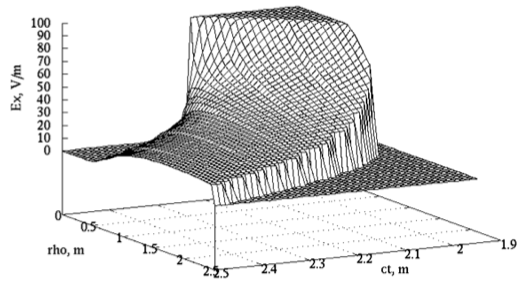
\includegraphics[scale=1.6]{MissileEffect}
\caption{Ефект електромагнітного снаряду ($ z = 2 $ м)} \label{fig:emp_rho}
\end{center} \end{figure}

На Рис.~\ref{fig:emp_rho} область $ S_1 $ зі сталим не нульовим значенням 
$ E_x $ компоненти поля спостерігаються лише для $ \rho < R $. За нею у 
часі наступає область $ S_2 $, де напруженість поля $ E_x $ поступово спадає 
на нуль. В області $ S_3 $ спостерігається $ E_x = 0 $.

Амплітуди всіх компонентів поля в області $ S_1 $ сталі, а значення 
цих амплітуд для $ E_x $ та $ H_y $ компонентів можна отримати з 
\eqref{eq:Exyz} та \eqref{eq:Hxyz} при $ \rho = 0 $:

\begin{equation*} \begin{aligned}
\vect{E} \{ S_1 \} = 
\vect{x_0} \frac{A_0}{4} 
\sqrt{\frac{\mu_0 \mu}{\epsilon_0 \epsilon}};
\end{aligned} \end{equation*}

\begin{equation*} \begin{aligned} 
\vect{H} \{ S_1 \} = \vect{y_0} \frac{A_0}{4}.
\end{aligned} \end{equation*}

Просторово-часова область з  постійними амплітудами напруженостей поля є 
одним з проявів ефекту електромагнітного снаряду і
зустрічається в багатьох роботах Содіна \cite{imp:Sodin1991, 
imp:Sodin1992-5, imp:Sodin1992-10, imp:Sodin1997}, роботах Ву 
\cite{imp:Wu1985, imp:Wu1987, imp:Wu1991}, в роботах Думіна
\cite{imp:Dumin1996} та в роботі Самсонова \cite{imp:Samsonov1986} але 
саме аналітичне значення амплітуди записано вперше, що є важливим для 
дослідження сильних полів.

Перехідна функція отримана без спрощень геометричної оптики, а отже 
справедлива для всіх точок спостереження ближньої зони. Отриманий результат 
дає змогу побачити форму електромагнітного імпульсу в залежності від 
азимутального кута при деякому $ z $ та $ \rho $, що лежать в ближній зоні.

З виразів для інтенсивності поля \eqref{eq:Exyz} та \eqref{eq:Hxyz} бачимо
центральну симетрію випромінювання відносно осі $ oZ $ для поперечних 
компонентів поля, отже достатньо дослідити лише залежність першій чверті.

\begin{figure}[h] \begin{center}
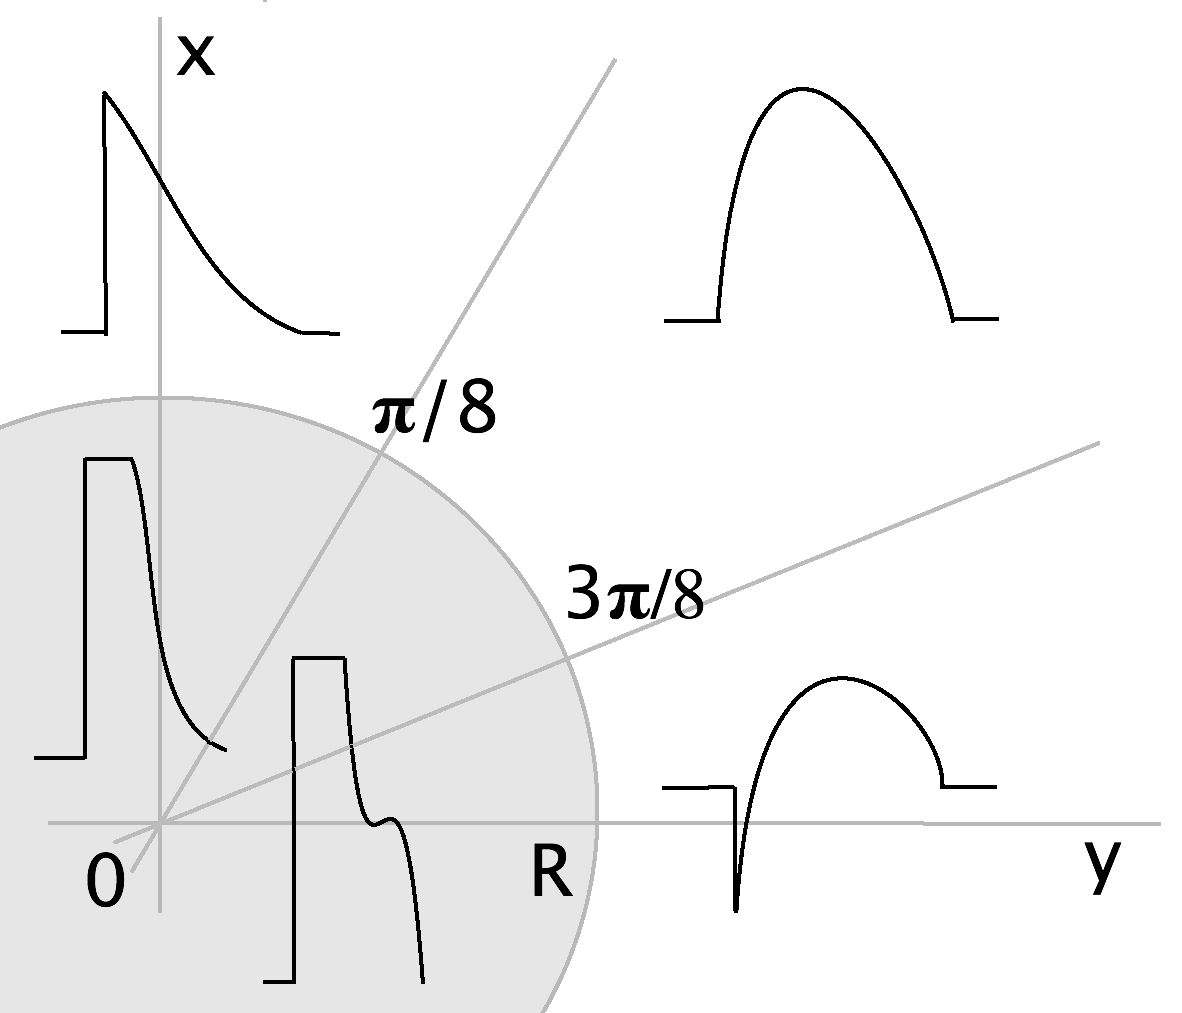
\includegraphics[scale=0.7]{LinearPulsShape}
\caption{Кутова залежність форми імпульсу ($ \rho = R/2 .. 2R $ м)} 
\label{fig:emp_shape}
\end{center} \end{figure}

На Рис.~\ref{fig:emp_shape} зображено залежність форми випроміненого 
імпульсу в залежності від кута спостереження в безпосередній близькості 
до джерела. Тут спостерігається вплив ефектів ближньої зони 
\cite{imp:Schantz2005}, при яких форма імпульсу залежить від напрямку 
поширення і від відстані. З рисунку §бачимо, що форма імпульсу в 
кожному напрямку в межах одного періоду симетрії унікальна, що можна 
використовувати в радарних та телекомунікаційних задачах 
(Дивись розділ~\ref{ch:neuron}).

За визначенням функції Ломмеля, інтеграли $ I_3 $ та $ I_4 $ є 
нескінченною сумою інтегралів по трьом функціям Бесселя 
(\eqref{eq:i3_pol_int}, \eqref{eq:i4_pol_int}). При аналізі магнітного 
поля на осі випромінювання помічаємо, що поперечне магнітне поле для 
області $ S_1 $ пропорційне по значенням з компонентами 
електричного. Для області $ S_3 $ поперечне магнітне поле описується 
рядом з поліномів Лягерра \eqref{eq:i3onaxis}.

\begin{figure}[h] \begin{center}
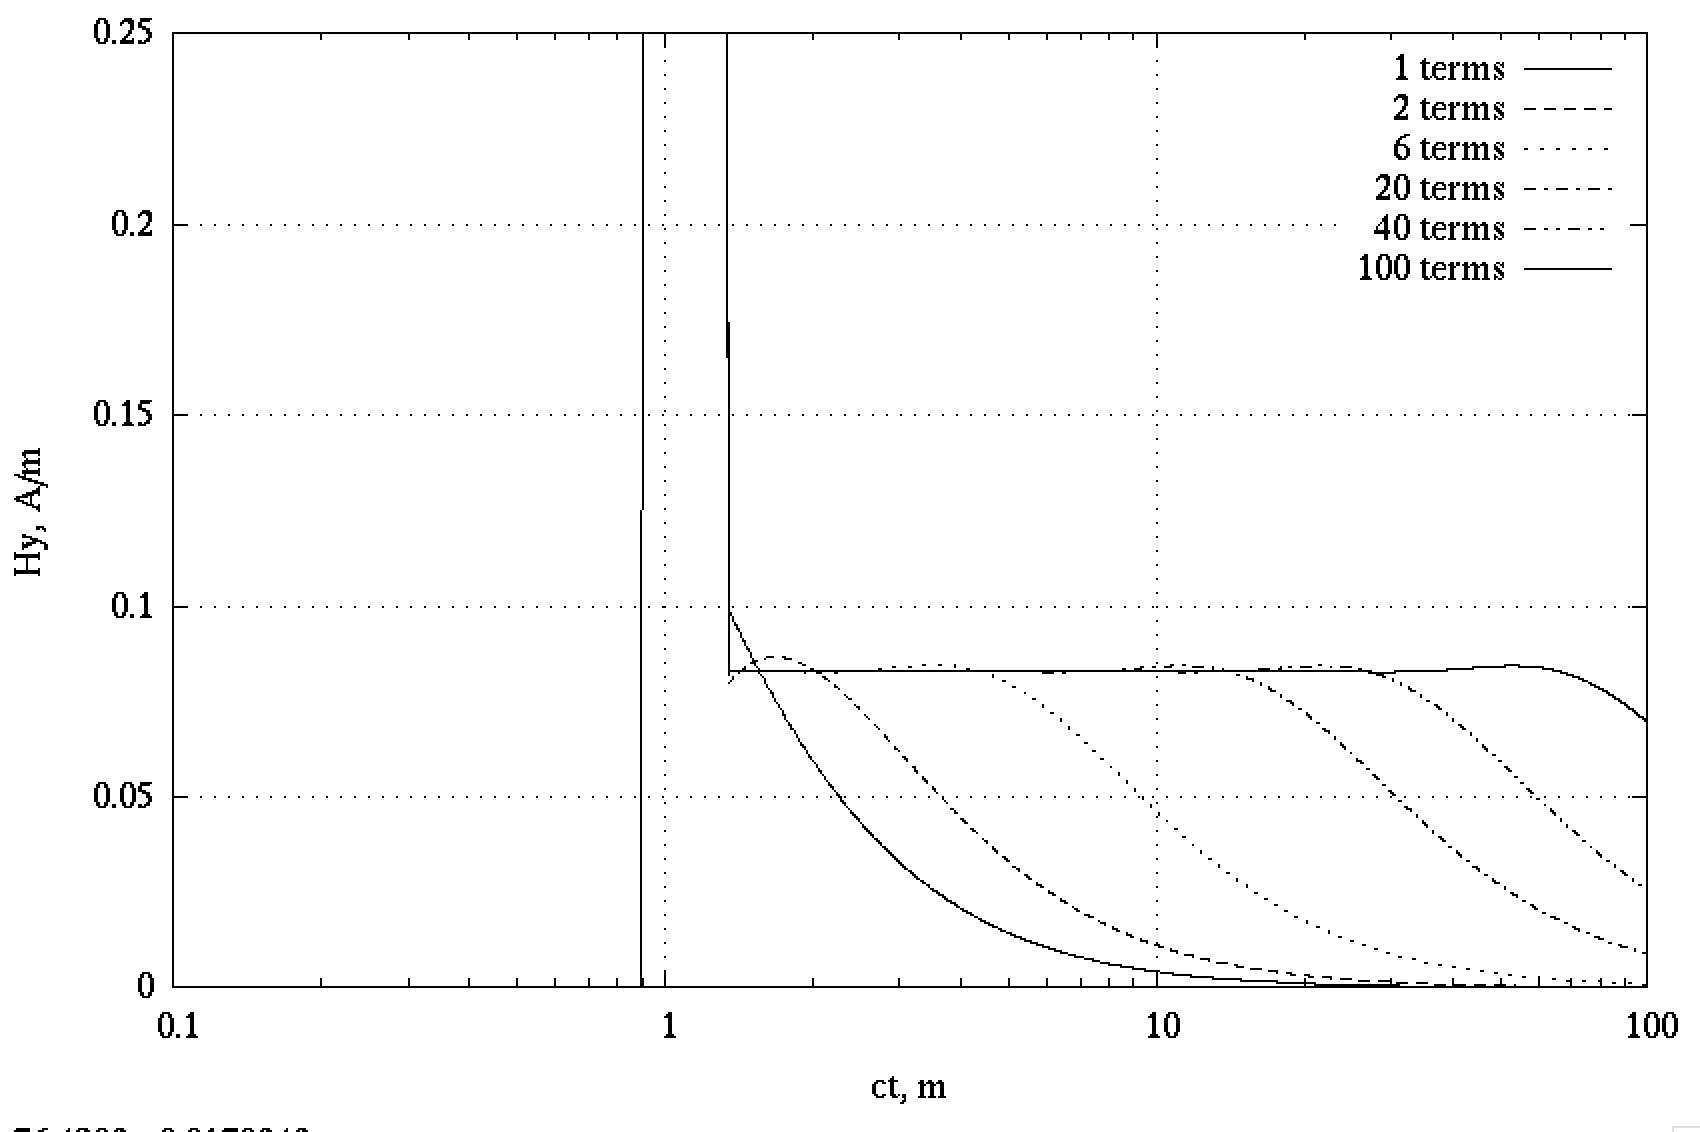
\includegraphics[scale=0.5]{SingulatiyFactorization}
\caption{Розклад сингулярності джерела} \label{fig:singulatiy_factorization}
\end{center} \end{figure}

На Рис.~\ref{fig:singulatiy_factorization} відображено процес сходження 
магнітної компоненти поля $ H_y $ при врахуванні різної кількості доданків
нескінченного поліному \eqref{eq:i3onaxis}. Бачимо, що з закінченням 
перехідного процесу наступає стаціонарне магнітне поле. Аналітично отриманий 
ряд сходиться дуже повільно. Можемо зробити висновок, що модовий базис 
погано підходить для опису стаціонарних процесів. Доданки вищих порядків 
мають значний вклад лише при пропорційно великому часі спостереження,
тобто, доданок $ m $ має внесок у значення функції $ H_z $ при $ ctm $.
На Рис.~\ref{fig:emp_h_z}, можемо оцінити згасання амплітуди 
магнітостатики з відстанню від джерела. На Рис.~\ref{fig:emp_h_z} 
спостерігається майже квадратичне згасання статичної 
компоненти з відстанню по $ z $. 

\begin{figure}[h] \begin{center}
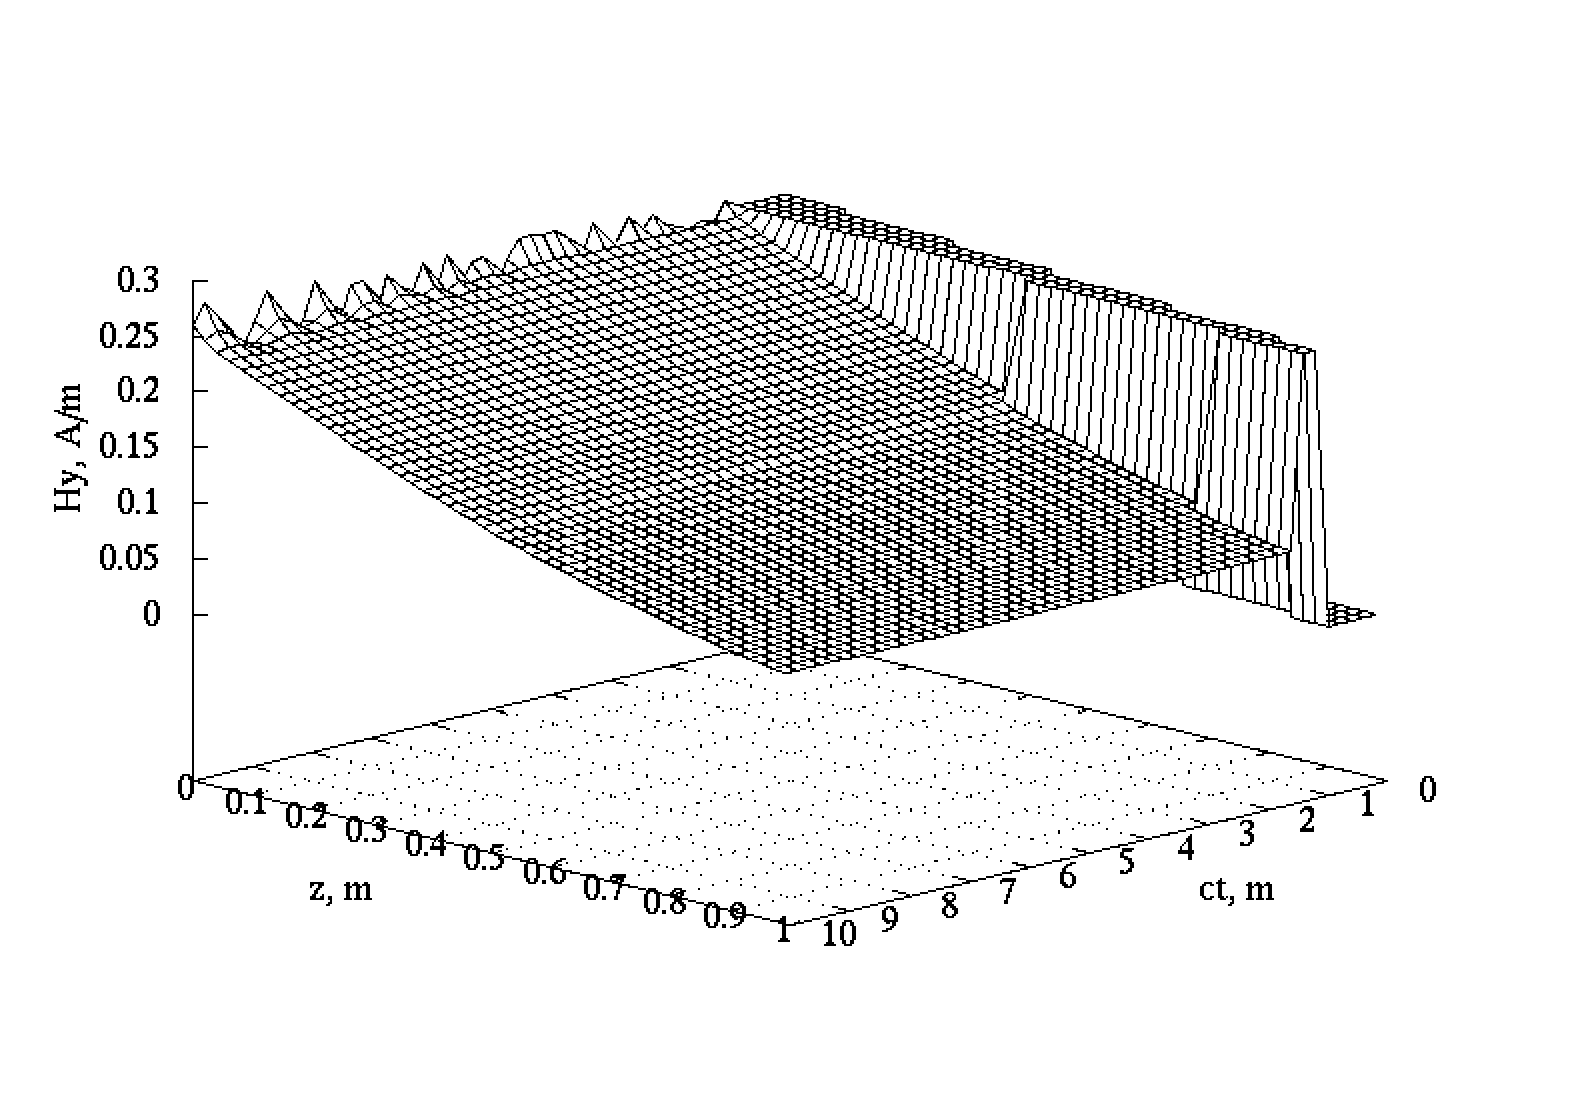
\includegraphics[scale=0.6]{StaticOnAxis}
\caption{Магнітностатичне поле ($ \rho = 0 $ м)} \label{fig:emp_h_z}
\end{center} \end{figure}

Розрахунок магнітних компонентів - розрахунок нескінченного 
поліному від невласних інтегралів з повільною збіжністю,
хоча і наближено, але дає змогу оцінити розподіл магнітного поля в 
залежності від віддаленням від джерела. З Рис.~\ref{fig:emp_h_z} також 
помічаємо погане сходження поліному Лягерра близько до сингулярності, тому 
результати числового розрахунку там не аналізуємо. Схожий результат було 
отримано методами частотної області для усталеного процесу випромінювання 
статичного магнітного поля пласким диском електричного струму в перших, 
роботах присвячених випромінюванню плаского диску \cite{imp:BaumIN0009}, 
де вирази магнітного поля також містять поліноми Лягерра, що свідчить про 
правильність отриманих результатів.

\begin{figure}[h] \begin{center}
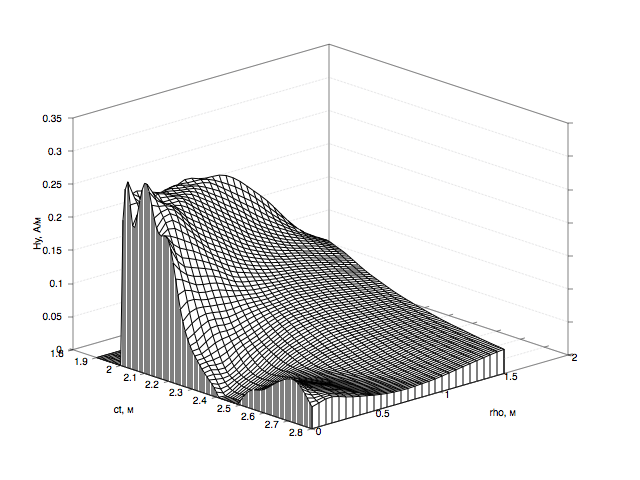
\includegraphics[scale=0.7]{LinearMagnetic}
\caption{Магнітностатичне поле ($ z = 2 $ м)} \label{fig:emp_h_rho}
\end{center} \end{figure}

На Рис.~\ref{fig:emp_h_rho} зображено зміну $ H_y $ за часом для 
різних значень $ 0 < \rho < 2R $ при $ z = 2R $. Знову спостерігаємо 
поступове згасання амплітуди магнітоcтатичного поля з відстанню.

З Рис.~\ref{fig:part_rad} та з аналітичних розв'язків для 
$ I_1, I_2, I_3, I_4 $ видно, що, знаходячись в області $ S_1 $, 
спостерігач не отримує ніякої інформації про джерело окрім його наявності.
Відсутність нової інформації дозволяє зробити висновок, що у всій області 
$ S_1 $ всі компоненти векторів напруженості поля мають стале значення.
Наприклад, $ H_x = 0 $, а $ H_y = A_0/4 $. Отже, користуючись відсутністю 
змін у джерелі в області спостереження $ S_1 $, визначивши значення для 
компоненти поля в одній точці, отримаємо розв'язок для всієї області $ S_1 $.  

Розглянемо поведінку поздовжньої магнітної компоненти $ H_z $. Користуючись
визначенням функції Ломмеля, поздовжню компоненту вектору напруженості 
магнітного поля можна записати у вигляді нескінченного ряду з невласних 
інтегралів \eqref{eq:i5series}. Для першого доданку значення інтегралу 
вдається знайти аналітично \eqref{eq:i50}. Також помічаємо, що при 
$ \rho = 0 $ поздовжнє магнітне поле теж відсутнє. Користуючись висновком 
про те, що в області $ S_1 $ всі компоненти поля мають постійні значення 
напруженості та тим, що в усіх точках, де $ 0 < ct - z \cup \rho = 0 $ 
поздовжнє магнітне поле відсутнє, робимо висновок, що $ H_z \{ S_1 \} = 0 $.
Таке твердження додатково підтверджується числовими розрахунками, а також
аналітичним розв'язком для першого доданку, який не протирічить отриманому
результату.

\begin{figure}[h] \begin{center}
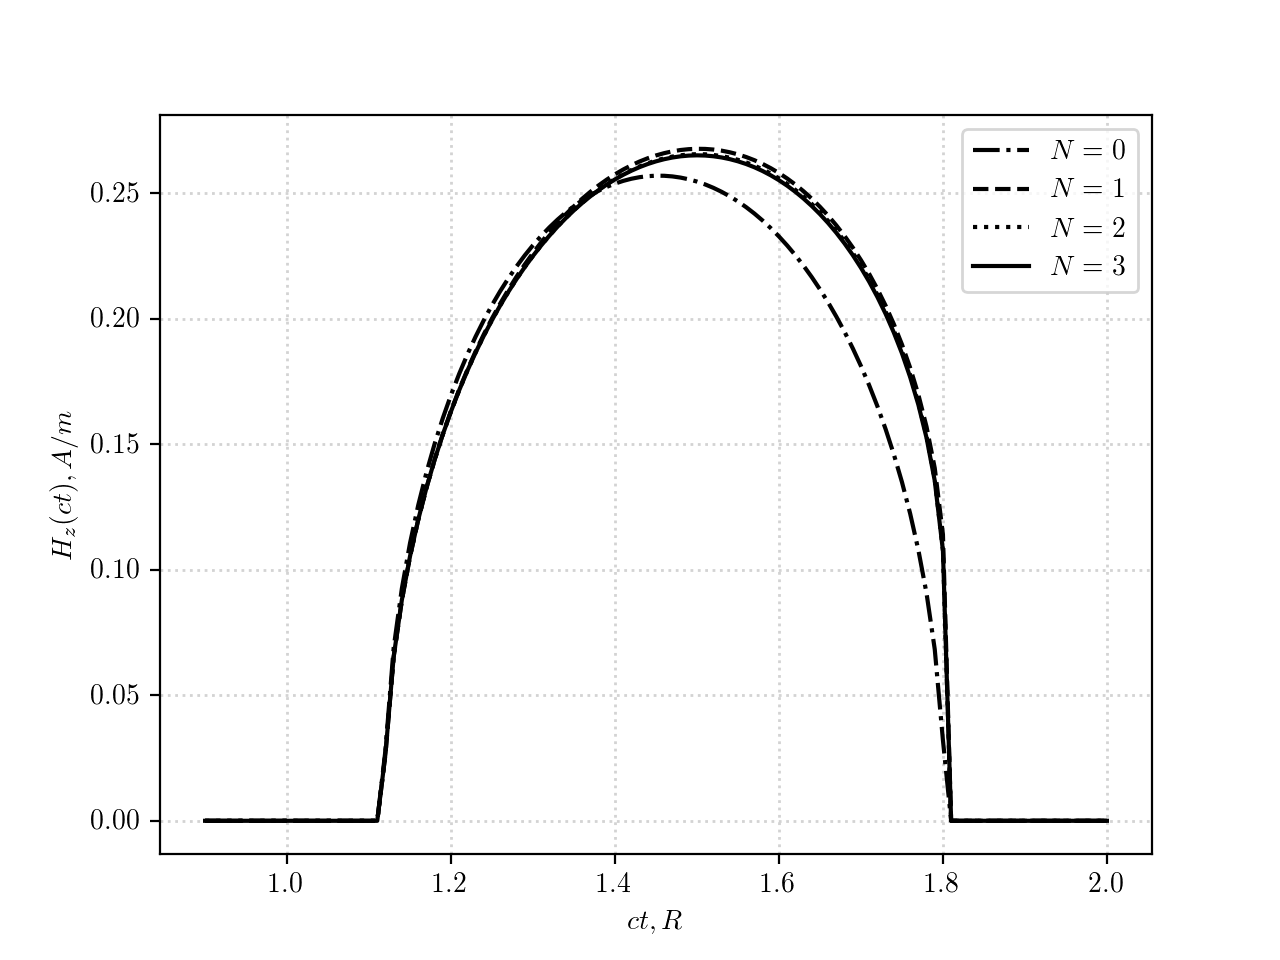
\includegraphics[scale=0.9]{Hz_terms}
\caption{Інтенсивність $H_z$ з плином часу в 
($\rho = R/2$, $\varphi = -\pi/2$, $z = R$) при 
різній кількості доданків $ N $} \label{fig:hz_terms}
\end{center} \end{figure}

На Рис.~\ref{fig:hz_terms} зображено поздовжню напруженість магнітного поля,
розрахованою чисельно за формулою \eqref{eq:i5series} для різної кількості 
врахованих доданків. Відносні похибка в розрахунку кожного невласного 
інтегралу не перевищує одного відсотку та отримано з застосуванням формули
Рунге \cite{imp:NumRecipes2007} та квадратурного правила Сімпсона 
\cite{imp:NumRecipes2007}. Помічаємо, що після двох врахованих 
доданків відхилення непомітне оку. Малий вплив доданків вищих порядків 
свідчить про те, що базис методу еволюційних рівнянь гарно підходить для 
опису нестаціонарних процесів.

Розглянемо співвідношення поздовжньої  магнітної компоненти $ H_z $ та 
поперечної електричної компоненти $ E_x $. На Рис.~\ref{fig:ex_vs_hz}
бачимо, що компонента $ H_z $ починається з затримкою відносно компоненти 
$ E_x $, а тривалість затримки співпадає з тривалістю ефекту 
електромагнітного снаряду. 

Плаский диск струму є апроксимацією ТЕМ джерела, а у вільному просторі 
поздовжня компонента повинна існувати, таким чином, затримку поздовжньої 
компоненти можна розуміти, як трансформацію ТЕМ хвилі в ТЕ з плином 
часу. Таким чином, ефект електромагнітного снаряду можна трактувати, як 
наслідок процесу формування хвилі у вільному просторі з TEM хвилі у рупорі.

\begin{figure}[h] \begin{center}
\includegraphics[scale=0.9]{Ex_vs_Hz}
\caption{$E_x$ і $H_z$ в ($\rho = R/2$, $\varphi = -\pi/2$, $z = R$)} 
\label{fig:ex_vs_hz}
\end{center} \end{figure}

В роботах Герца \cite{imp:Hertz1938} зустрічається твердження, що 
випромінює не антена, а простір довкола неї. Саме це і спостерігається в 
області електромагнітного снаряду: через відсутність причинного зв'язку з 
краєм рупора, хвиля знаходячись у вільному просторі, має властивості хвилі у 
ТЕМ хвилеводі. Тобто, протягом тривалості електромагнітного сняряду ми 
спостерігаємо перетворення хвилі у хвилеводі на хвилю у вільному просторі, 
яка не може існувати без поздовжньої компоненти ($ H_z \neq 0 $) 
\cite{imp:Borisov1991, imp:Harmuth1985}. Також відмітимо, що форма часової 
залежності збуджувального імпульсу не впливає на затримку у появі $ H_z $
компоненти поля. Вона залежить лише від наявності в апертурі антени
поверхні рівних фаз та спостерігатиметься в усіх точках простору, що 
знаходиться на нормалі до цієї "пласкої" частини фронту в апертурі.

Таким чином, можемо узагальнити твердження Герца для нестаціонарного 
процесу: поширення хвилі у вільному просторі почнеться з моменту, 
коли спостерігач дізнається про те, що розподіл струму в апертурі просторово
змінюється, а до цього, спостерігається той самий процес, що і у 
внутрішньому просторі антени. Звісно, такий ефект досягається за рахунок 
апертури рівних фаз і за рахунок часової залежності збуджувального струму у 
вигляді ступеневої функції Хевісайда, що неможливо для реальних джерел через 
похибки у виготовлені лінз і наявність передімпульсних коливань генератора.

Також, узагальнимо фізичний смисл розділу областей випромінювання: 
$ S_1 $ - область формування хвилі у вільному просторі, $ S_2 $ - область 
несталого (перехідного) процесу випромінювання, $ S_3 $ - область
усталеного процесу.

%%%%%%%%%%%%%%%%%%%%%%%%%%%%%%%%%%%%%%%%%%%%%%%%%%%%%%%%%%%%%%%%%%%%%%%%%%%%%%
\section{Збудження імпульсом довільної форми}

Оцінимо вплив ефектів ближньої зони на поле, що породжене пласким диском 
електричного струму на прямокутний збуджувальний імпульс тривалістю 
$ \tau_0 $, тобто вмикання струму до амплітуди $ A_0 $ Вольт і послідовне 
його вимкнення з затримкою $ \tau_0 $ секунд:

\begin{equation}
\vect{j} (r,t) = \vect{j_0} (r,t) - \vect{j_0} (r,t-\tau_0),
\end{equation}
%
де $ \vect{j_0} $ - струм, що породжує електричну $ \vect{E_0} $ і магнітну 
$ \vect{H_0} $ перехідні функції. Таким чином, користуючись принципом 
суперпозиції маємо:

\begin{equation}
\vect{E} (r,t) = \vect{E_0} (r,t) - \vect{E_0} (r,t-\tau_0).
\end{equation}

\begin{table}[ht]
\caption{Епюри форми імпульсного електричного поля породженого LIRA, 
яке збуджується прямокутним імпульсом тривалістю R}
\label{tab:meander_shape}ц
\centering
\begin{tabular}{cccc}

& $ \varphi = 0 $ & $ \varphi = \pi/4 $ & $ \varphi = \pi/2 $ \\

$ \rho = 0 $ &
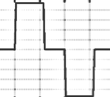
\includegraphics[scale=2]{meander/00_00} & 
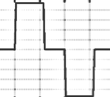
\includegraphics[scale=2]{meander/00_45} & 
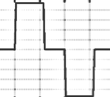
\includegraphics[scale=2]{meander/00_90} \\

$ \rho < R $ &
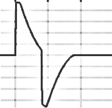
\includegraphics[scale=2]{meander/05_00} & 
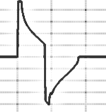
\includegraphics[scale=2]{meander/05_45} & 
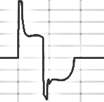
\includegraphics[scale=2]{meander/05_90} \\

$ \rho > R $ &
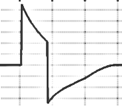
\includegraphics[scale=2]{meander/20_00} & 
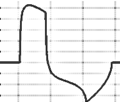
\includegraphics[scale=2]{meander/20_45} & 
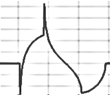
\includegraphics[scale=2]{meander/20_90} \\

\end{tabular}
\end{table}

В Таб.~\ref{tab:meander_shape} епюрами наведено залежність 
форми випроміненого імпульсу антени типу LIRA при прямокутному 
збуджені від напрямку випромінювання зі збереженням масштабу за 
часом та без збереження амплітуди.

Тривалість перехідної функції $ \vect{E_0} $ на осі випромінювання 
$ \sqrt{z^2+R^2} - z $, а її максимальне значення досягається при малих 
відстанях до апертури та наближається до $ R $. Тому, якщо затримка перед 
вимкненням струму $ c \tau_0 $ триваліша за $ R $, накладання відгуків 
на вмикання струму та на його вимикання не спостерігається. Як відомо, саме 
це накладання є причиною мінливості форми імпульсу у ближній зоні. Якщо, 
також, врахувати $ \rho \neq 0 $, то можна отримати, що тривалість імпульсу 
$ \tau_0 > 2R/c $, коли накладання буде відсутнє для довільної 
точки спостереження.

Користуючись методикою інтегрування Дюамеля, \cite[ст. 40]{imp:Kharkevich1950} 
знайдемо поле від антени з відомою перехідною функцією $ \vect{E_0} (r,t) $, 
що збуджено сигналом з плавною часовою залежністю $ f(t) $ при 
максимальній амплітуді збуджувального струму $ A_0 $ В:

\begin{equation} \label{eq:duhamel}
\vect{E} = \int_0^t \derivat{f}{\tau} \vect{E_0} (t - \tau) d \tau.
\end{equation}

Інтеграл \eqref{eq:duhamel} є узагальненням принципу суперпозиції, а отже
працюватиме лише для лінійної залежності електричної індукції від 
напруженості поля. Проте, його використання доцільне для вивчення 
напруженості імпульсного поля, яка при накладанні може викликати 
необхідність врахування нелінійних ефектів, на кшталт, пробою в сильних полях.

Розглянемо в якості форми збудження плавне наростання амплітуди струму до 
значення $ A_0 $ протягом $ \tau_0 $ за метрикою 1-99 risetime у вигляді 
сигмоїдальної функції.

\begin{figure}[h] \begin{center}
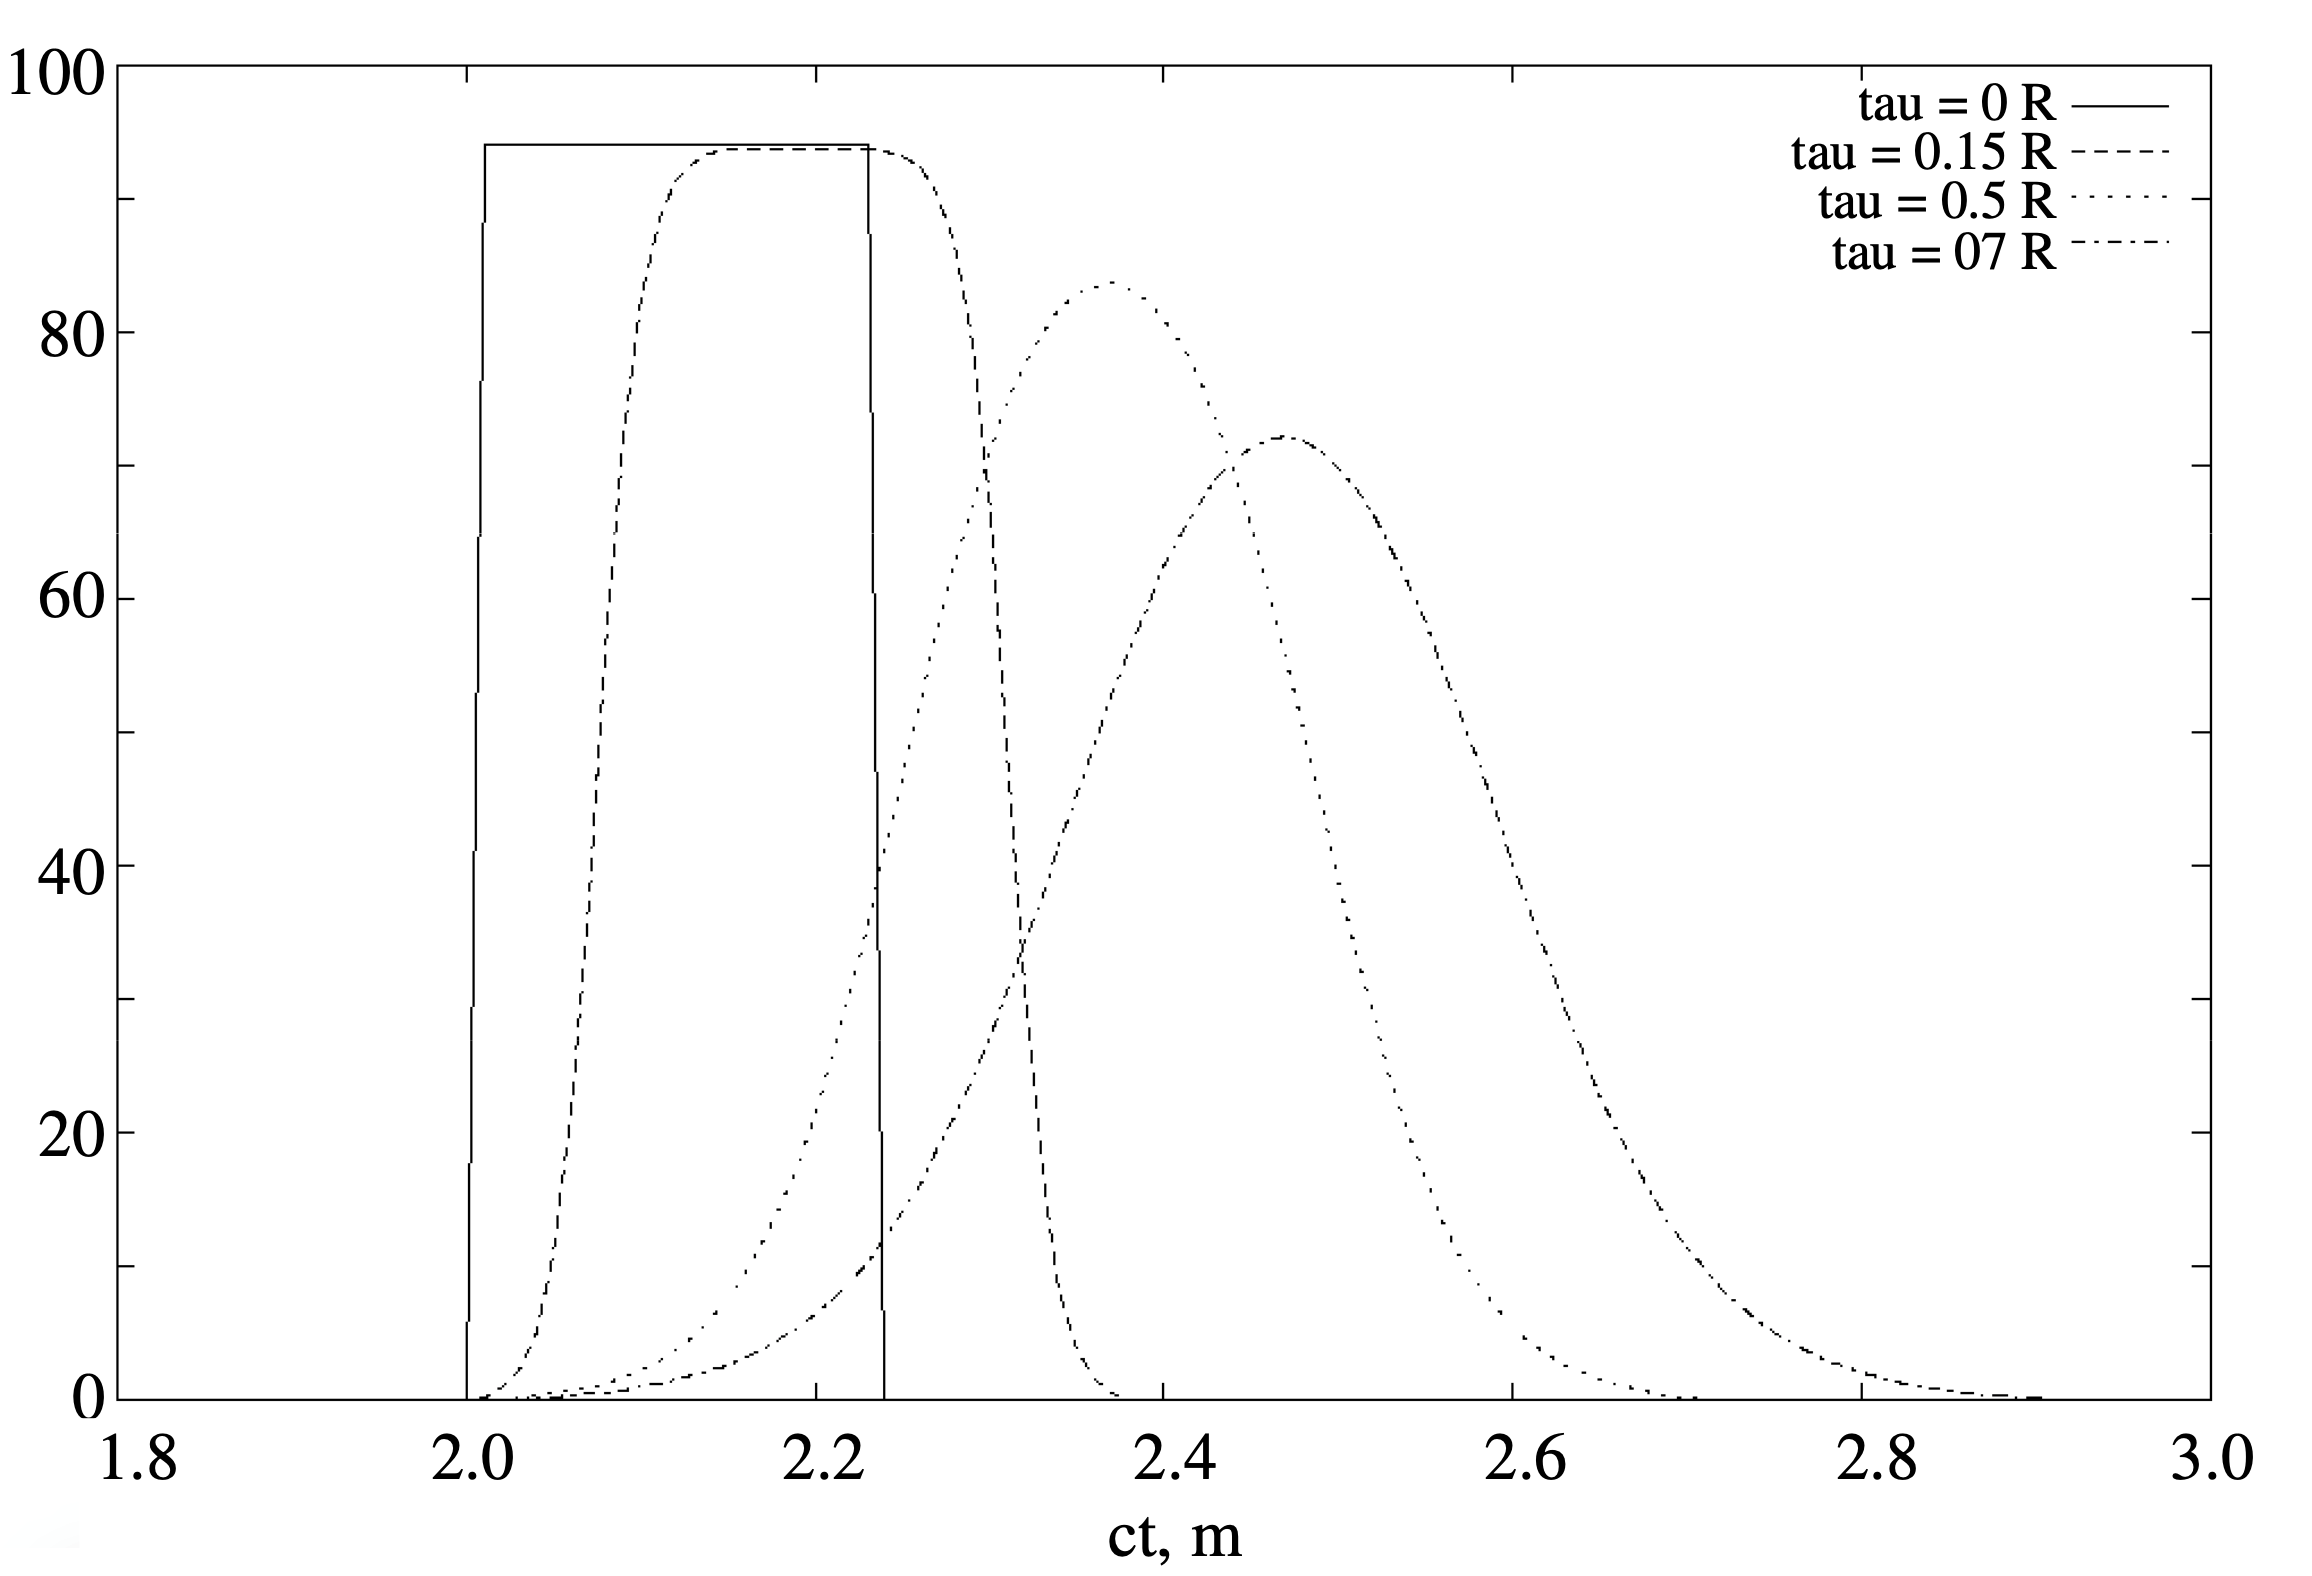
\includegraphics[scale=0.4]{Sigmoidal}
\caption{$ E_x $ компонента поля від сигмоїдального збудження}
\label{fig:ex_sigmoidal}
\end{center} \end{figure}

Результати, представлені на Рис.~\ref{fig:ex_sigmoidal}, сходяться з 
експериментальними дослідженнями отримані незалежно Баумом та Ву.

Тепер розглянемо збуджувальний сигнал у вигляді $ f(t) = \sinc t $.
Така часова залежність збудження для плаского диску породжує імпульсне
швидко-осцилююче поле. Розглянемо інтерференцію цього поля в ближній зоні.
На Рис.~\ref{fig:ex_sinc} зображено залежність напруженості електричного 
поля $ E_x $ від часу для двох точок спостереження.

\begin{figure}[h] \begin{center}
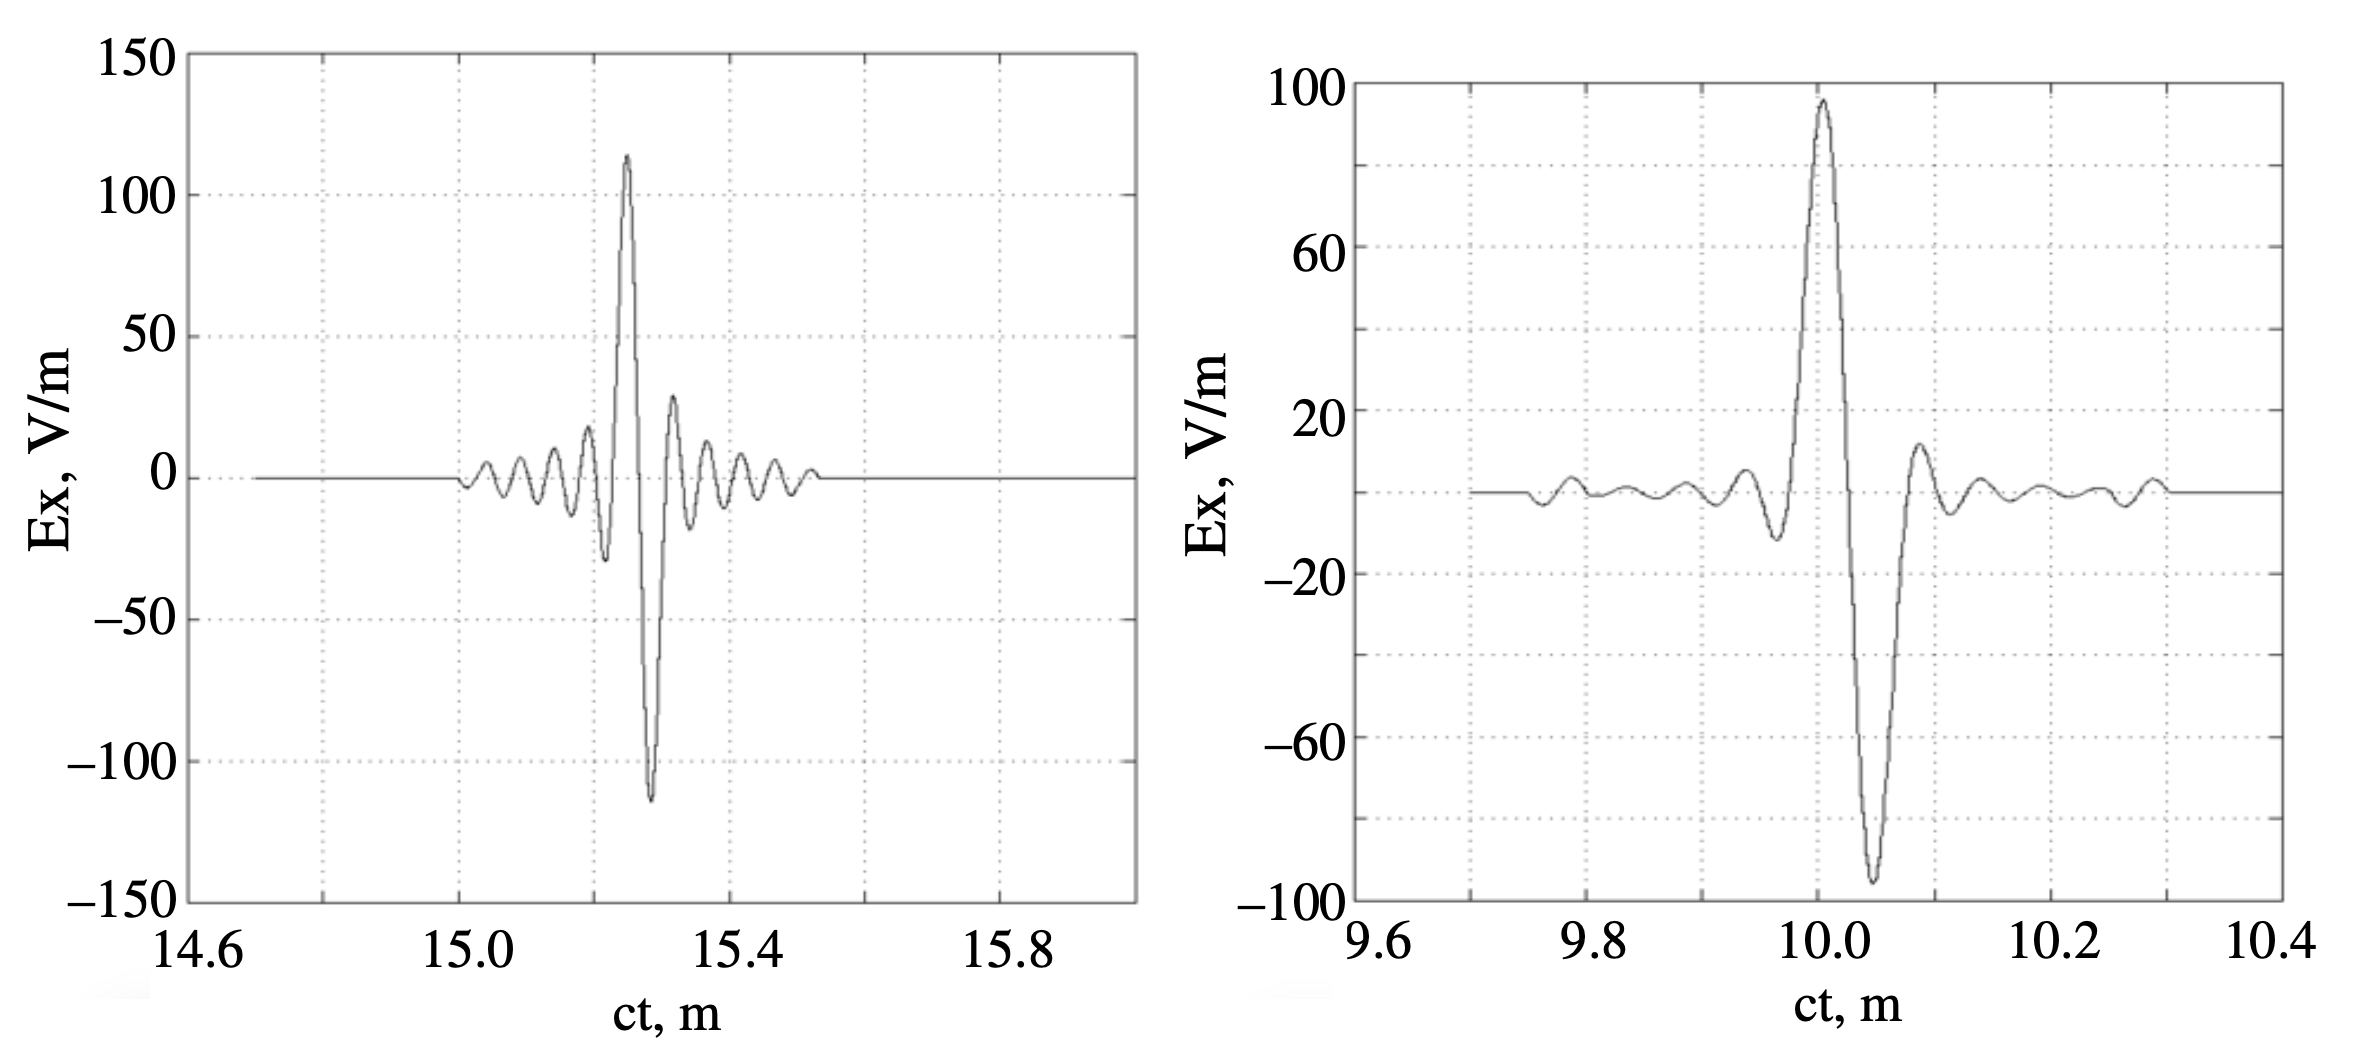
\includegraphics[scale=0.4]{Sinc}
\caption{$ E_x $ компонента поля від $ \sinc t $ збудження}
\label{fig:ex_sinc}
\end{center} \end{figure}

З Рис.~\ref{fig:ex_sinc} бачимо, що на більшому віддалені від джерела, 
максимальна напруженість поля більша за максимальну напруженість, що була 
досягнута при менших відстанях. При накладанні перехідних функцій початку 
збудження та дзеркального його продовження спостерігається протифазне 
накладання, що з відстанню переходить у синфазне і амплітуда сигналу 
збільшується в межах $ 20\% $. Таким чином, при роботі з сильними 
швидко-осцилюючими імпульсними полями цей ефект треба враховувати, щоб 
уникнути електричного пробою в межах короткотривалих піках напруженості.
Звісно, перехідну функцію LIRA було отримано з припущенням відсутності 
втрат при поширенні, отже реальний вплив цього накладання виявиться 
меншим.

Відомо, що в дальній зоні форма сигналу, що випромінюється, схожа на похідну
від часової залежності збуджувального струму. Розглянемо збудження з 
часовою залежністю  у вигляді гаусіана та похідної від гаусіана, але тої ж 
тривалості. Спробуємо знайти такі точки спостереження, де форми 
випромінених імпульсів цих різних збуджень будуть візуально, а відповідно і 
за спектром схожі.

\begin{figure}
\subfloat[Збудження у вигляді похідної від гаусіана]{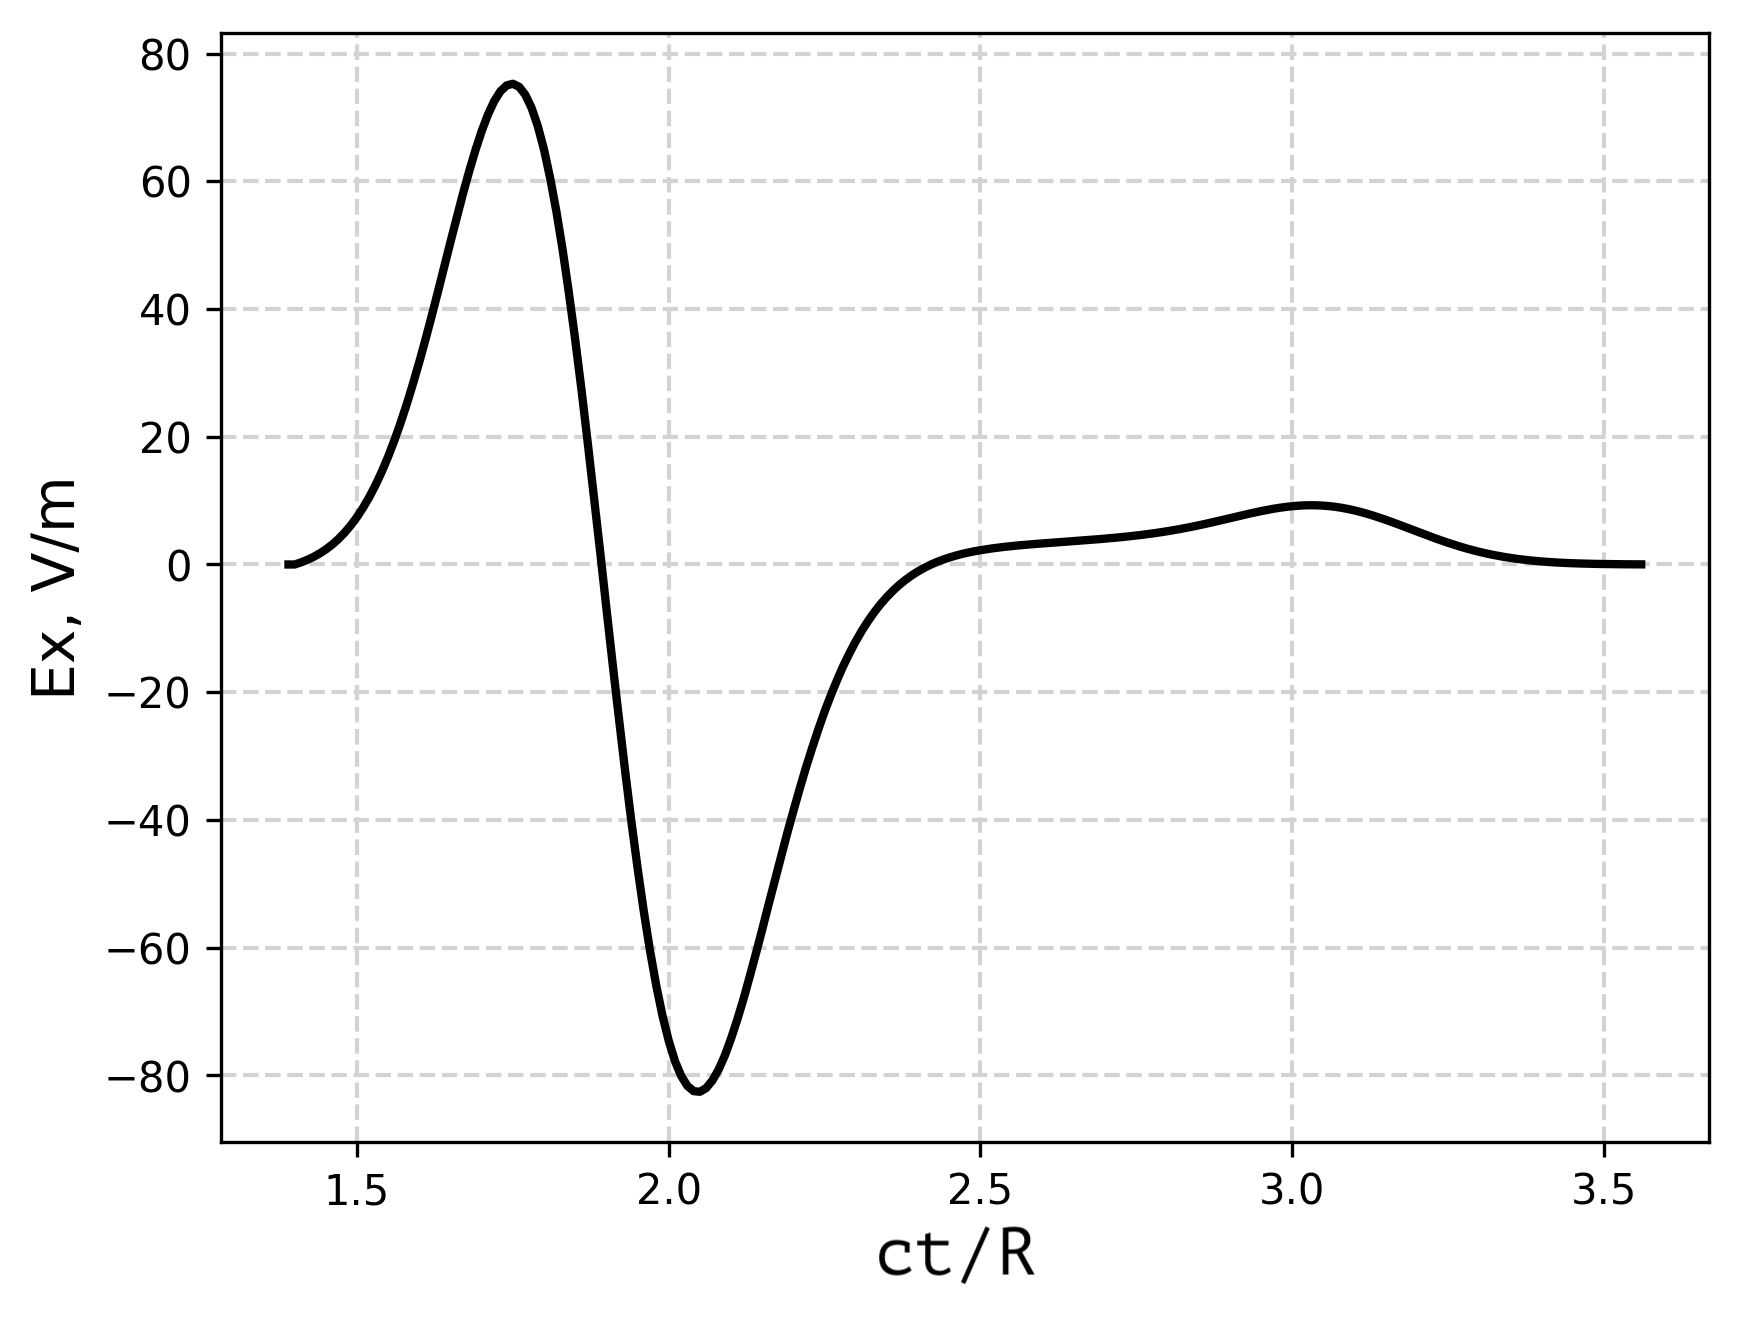
\includegraphics[width = 3in]{gauss1}} 
\subfloat[Збудження у вигляді гаусіана]{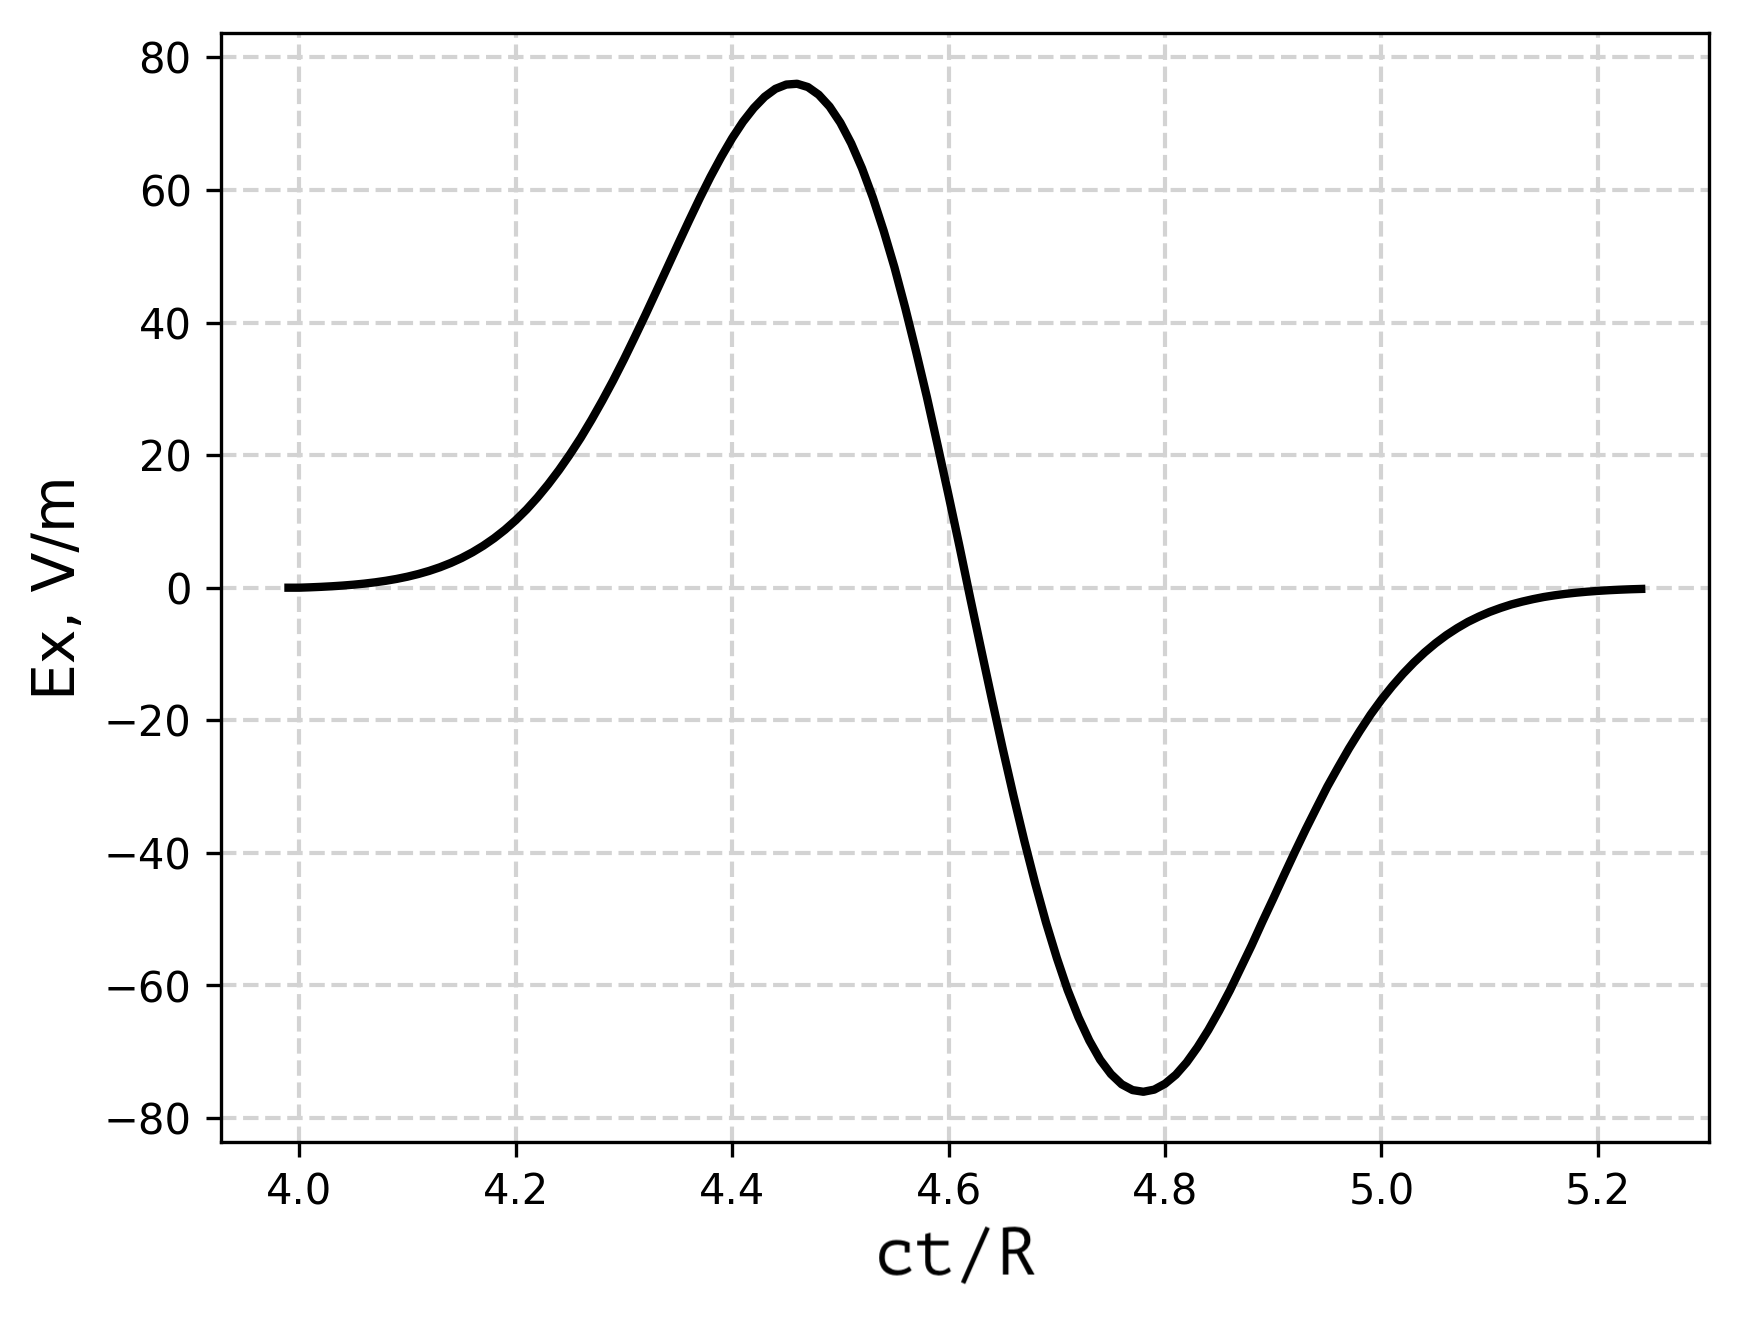
\includegraphics[width = 3in]{gauss2}}
\caption{Електричне поле антени типу LIRA збуджене струмом з 
різними часовими залежностями}
\label{fig:gauss_shape}
\end{figure}

На Рис.~\ref{fig:gauss_shape} зображено напруженість електричного поля, 
що породжено LIRA із часовою залежністю збудження у формі функції Гауса (а), 
та у формі її похідної (б). Рисунок ілюструє, що в ближній зоні можна знайти
такі точки спостереження, де різне збудження породить поле майже однакового 
вигляду. Як вже зазначалось, в дальній зоні, а також у більшості випадків у 
ближній зоні, форма випроміненого імпульсу є похідною від форми збуджувального 
імпульсу, але якщо спостерігати поле збуджене, струмом з часовою залежністю у 
вигляді похідної гаусінана в точці $ \rho = R/2, \varphi = \pi/4, z = R $
електромагнітний імпульс матиме такий вигляд, наче ми спостерігаємо імпульс, 
збуджений іншим струмом. Невелика різниця між формами сигналів може легко 
губитись в шумах та зробить процес розрізнення імпульсів стандартними 
алгоритмами FPGA неможливим.

%%%%%%%%%%%%%%%%%%%%%%%%%%%%%%%%%%%%%%%%%%%%%%%%%%%%%%%%%%%%%%%%%%%%%%%%%%%%%%
\section*{Висновки до розділу \ref{ch:linear}}

Побудовано аналітичне розв'язання у вигляді кусково визначеної функції для 
задачі випромінювання круглої апертури при нестаціонарному збуджені у 
вигляді прямокутної функції. Розв'язок отримано без наближення дальньої 
зони та визначено для всіх точок спостереження в кожен момент часу. 
Використання моделі круглої апертури, як моделі антен типу LIRA перевірено 
на експериментальних даних в окремих точках та на даних отриманих методом 
FDTD з комерційного електромагнітного симулятора CST Studio.

Отримане розв'язання задачі випромінювання плаского диску при збуджені у 
вигляді функції Хевісайда в лінійному наближенні має чітку про-\\
сторово-часову 
зональність та ілюструє твердження Фарадея, що випромінює не антена, а 
простір довкола неї. Отримані області випромінювання наступають послідовно 
для довільної точки спостереження. Остання за часом настання область $ S_3 $ 
відповідає стаціонарному (усталеному) процесу випромінювання, коли всі точки 
апертури поєднані зі спостерігачем за принципом причинності. Настанню 
усталеного процесу передує область деякого транзитивного процесу $ S_2 $, 
поки поле від всієї апертури не досягне спостерігача. Найпершою для 
спостерігача просторово-часовою областю випромінювання в прожекторній зоні 
круглої апертури настає область електромагнітного снаряду $ S_1 $, де з 
хвилі у ТЕМ рупора формується ТЕ хвиля у вільному просторі.

%\textcolor{red}{TODO: можна строго порiвняти дiаграму спрямованостi отриману в
%	часовiй областi з дiаграмою Баума, а також оцiнити її вiдхилення в ближнiй
%	зонi}


% \textcolor{red}{ТОDО: Врахування краєвих ефектів випромінювання. 
% Шматько Александр Александрович на защите Лены Овсянниковой 
% замечал что, для того чтоб задачу можно было назвать апертурной, 
% нужно учеть в модели краевое излечение}
% ANS: тема майбутніх досліджень, усклавднить, уникли тому що резистори

Результати цього розділу відображені в роботах автора 
\cite{my:Telecom2018, my:UKRCON2017, my:UWBUSIS2018, my:UKRCON2019}.

\chapter{Розповсюдження випромінювання плаского диску в нелінійному середовищі}
\label{ch:nonlinear}

%%%%%%%%%%%%%%%%%%%%%%%%%%%%%%%%%%%%%%%%%%%%%%%%%%%%%%%%%%%%%%%%%%%%%%%%%%%%%%%%
\section{Матеріальні рівняння, як модель нелінійного середовища}

Взаємодію поля крізь середовище, завдяки теорії суперпозиції, можна
представити у вигляді додаткового стороннього джерела поля, що буде 
просторово розподілене в усій області розповсюдження породжувальної 
сильної хвилі. Для сильних хвиль, що мають імпульсну природу 
крім просторового розподілу доводиться розглядати, ще і причинний 
зв'язок. Назвемо таке джерело вторинним.

Розглянемо модель, де характер взаємодії електромагнітного поля і середовища 
задається в матеріальних рівняннях, де поляризація та намагніченість 
розглядаються, як \textcolor{red}{джерела} електромагнітної індукції.

\begin{equation*}
\vect{D} = \epsilon_0 \vect{E} + \vect{P} \left( \vect{E}, \vect{H} \right) =
\epsilon_0 \vect{E} + \epsilon_0 \chi_e \left( \vect{E}, \vect{H} \right)
\end{equation*}

\begin{equation*}
\vect{B} = \mu_0 \vect{H} + \mu_0 \vect{M} \left( \vect{E}, \vect{H} \right) =
\mu_0 \vect{H} + \mu_0 \chi_m \left( \vect{E}, \vect{H} \right)
\end{equation*}

Виключимо з розглядання гіротропні і не-хіральні середовища, тоді взаємний 
вплив магнітної та електричної індукції зникне і вектор поляризації стане 
функцією лише електричної напруженості, а намагніченість - лише магнітної
напруженості. Також, клас середовищ, що розглядається, обмежимо сталими, 
однорідними та ізотропними властивостями. Розглянемо середовище з лінійною 
магнітною індукцією

\begin{equation}
\vect{B} = \mu_0 \vect{H} + \mu_0 \chi_m \left( \vect{H} \right) =
\mu_0 \left( \chi_m + 1 \right) \vect{H} = \mu_0 \mu \vect{H}
\end{equation}
%
та нелінійною електричною індукцією

\begin{equation} \label{eq:d_voltera}
\vect{D} = \epsilon_0 \vect{E} + \epsilon_0 \chi_e \left( \vect{E} \right) = 
\epsilon_0 \vect{E} + \epsilon_0 \sum_{k=1}^{\infty} \int_0^t
\chi_e^{(k)} (\tau) \vect{E}^k (\tau) d \tau,
\end{equation}
%
де $\chi_e^{(k)} (t) $ коефіцієнти розкладу Вольтера нелінійної функції 
$ \chi_e $ по параметру $ \vect{E} $.

Розклад Вольтера ілюструє затримку у відгуках середовища на помірно сильні 
збудження. Розклад \eqref{eq:d_voltera} може застосовуватись у випадках,
коли породжуюче поле розповсюджуватись у середовищі не змінює його квантовий
стан. Такий тип нелінійності називається параметричним та випадку слабкої 
нелінійності. Тепер припустимо, що нелінійні ефекти в середовищі, що 
розглядається, не є інерційними за часом та породжують індукційний відгук 
миттєво. Тоді, від розкладу в ряд Вольтера перейдемо до Тейлорівського 
ряду, як моделі нелінійності:

\begin{equation} \label{eq:d_teilor}
\vect{D} = \epsilon_0 \vect{E} + 
\epsilon_0 \sum_{k=1}^{\infty} \chi_e^{(k)} \vect{E}^k (t).
\end{equation}

Розглянемо другий доданок в виразі \eqref{eq:d_teilor}: з точки зору 
матеріальних рівнянь він описує поляризаційні властивості середовища,
а згадуючи властивість симетрії вектору поляризації 
$ \vect{P} \left( \vect{E} \right) = - \vect{P} \left( - \vect{E} \right) $
лише непарні доданки ряду Тейлора можуть бути не нульовими. Також,
відокремивши лінійну поляризацію отримаємо вираз

\begin{equation} \label{eq:d_teilor_odd}
\vect{D} = \epsilon_0 \epsilon \vect{E} + 
\epsilon_0 \sum_{k=1}^{\infty} \chi_e^{(2k+1)} \vect{E}^{2k+1} (t).
\end{equation}

Для широкого класу прикладних задач \textcolor{red}{[UPSALA]} розглядається
лише перший нелінійний доданок розкладу. Таким чином отримаємо кубічну 
нелінійну складову вектору поляризації, що зустрічається в оптиці під 
назвою нелінійна поляризація Керра

\begin{equation} \label{eq:d_kerr}
\vect{D} = 
\epsilon_0 \epsilon \vect{E} + \epsilon_0 \chi_e^{(3)} \vect{E}^{3} = 
\epsilon_0 \epsilon \vect{E} + \vect{P}^\prime.
\end{equation}

Хоча розклад в ряд тейлора \eqref{eq:d_teilor_odd} не гарантує зменшення 
впливу кожного наступного доданку, тобто $ \chi_e^{(i)} < \chi_e^{(i+1)} $
на практиці врахування лише першого нелінійного доданку найчастіше дає
гарну точність до наближення слабкої нелінійності і врахуванням доданків
вищих порядків нехтують.

\textcolor{red}{ Які нелінійні ефекти спостерігаються в 
керрівському середовищі?}

Перша складова вектору електричної індукції \eqref{eq:d_kerr} відповідає 
полю при лінійному наближенні $ \vect{E} $, що породжене деяким 
струмом $ \vect{J} $, а другий доданок відповідає нелініному Керрівському 
відгуку середовища, який згідно з принципом суперпозиції, можна розглянути, 
як деяке поле $ \vect{E}^\prime $, породжене додатковим розподілом струму 
зміщення $ \vect{J}^\prime $ (далі вторинне джерело). Тоді, відповідно до
аналогії зі струмом зміщення, індукований нелінійний вторинний струм

\begin{equation} \label{eq:j_kerr}
\vect{J^\prime} = \partder{\vect{P}^\prime}{t} = 
\epsilon_0 \chi_e^{(3)} \partder{\vect{E}^3}{t}.
\end{equation}

Згідно описаної моделі, деяке стороннє джерело $ \vect{J} $ породжує 
імпульсне електромагнітне поле $ \vect{E} $ та $ \vect{H} $ розраховане
з припущенням лінійності електромагнітної індукції. Це лінійне поле, 
розповсюджуючись зі втратами крізь середовище, формує струм зміщення 
$ \vect{J}^\prime $, який в свою чергу є джерелом поля $ \vect{E}^\prime $ 
та $ \vect{H}^\prime $. Тоді, нелінійна самодія хвилі крізь середовище, 
згідно принципу суперпозиції $ \vect{E} + \vect{E}^\prime $ та 
$ \vect{H} + \vect{H}^\prime $.

Вторинне джерело $ \vect{J}^\prime $ забирає енергію породжуючої хвилі та 
формується частиною енергії втрат $ \vect{E} $, що характеризують середовище.

\textcolor{red}{ Розглянута модель, не пояснює нелінійні ефекти в вакуумі. 
Можливо, що природа нелінійних ефектів значно глибша і їх ефект впливає на 
характер енергетичної взаємодії та змінює простір. Відповідно довжина вектора 
в декартовому сенсі втрачає зміст. }

Вторинне джерело поля не є реальним джерелом, в прямому розумінні. 
Джерело $ \vect{J^\prime} $ наближено моделює нелінійну природу фізичних 
явищ розповсюдження сильних електромагнітних хвиль. Згадуючи всі обмеження,
які були велені при побудові моделі зазначимо властивості середовищ для 
яких цю модель можна застосовувати... \textcolor{red}{TODO...}

Розглянемо в якості породжувальної хвилі $ \vect{E} $ поле породжене 
пласким диском електричного струму з часовою залежністю у вигляді 
функції Хевісайда - моментальний стрибок амплітуди струму від нуля до 
значення $ A_0 $.

\textcolor{blue}{ \begin{equation*} 
\vect{J^\prime} = 
\vect{\rho_0}    \partder{}{t} P_\rho^\prime    \left( \vect{E} \right) + 
\vect{\varphi_0} \partder{}{t} P_\varphi^\prime \left( \vect{E} \right) + 
\vect{z_0}       \partder{}{t} P_z^\prime       \left( \vect{E} \right) 
\end{equation*} }
%
\textcolor{blue}{ \begin{equation*}
\vect{P^\prime} \left( \vect{E} \right) = \epsilon_0 \chi_e^{(3)} 
\dotprod{ \vect{E} }{ \vect{E} } \cdot \vect{E} 
\end{equation*} }
%
\textcolor{blue}{ \begin{equation*} \begin{aligned}
\vect{P^\prime} \left( \vect{E} \right) = 
\frac{ {A_0}^3 \epsilon_0 \chi_e^{(3)} }{ 8 } \left( \frac{\mu_0 \mu}
{\epsilon_0 \epsilon} \right)^{3/2} \left( {I_1}^2 \cos^2 \varphi + 
\left( I_2 - I_1 \right)^2 \sin^2 \varphi \right) \cdot \\ 
\cdot \Big( \vect{\rho_0} I_1 \cos \varphi - 
\vect{ \varphi_0 } \left( I_2 - I_1 \right) \sin \varphi \Big)
\end{aligned} \end{equation*} }
%
\textcolor{blue}{ \begin{equation*} \begin{aligned}
\vect{P^\prime} \left( \vect{E} \right) = 
\frac{ {A_0}^3 \epsilon_0 \chi_e^{(3)} }{ 8 } \left( \frac{\mu_0 \mu}
{\epsilon_0 \epsilon} \right)^{3/2} \left( {I_1}^2 \cos^2 \varphi + 
\left( I_2 - I_1 \right)^2 \sin^2 \varphi \right) \cdot \\ 
\cdot \Big( \vect{\rho_0} I_1 \cos \varphi - 
\vect{ \varphi_0 } \left( I_2 - I_1 \right) \sin \varphi \Big)
\end{aligned} \end{equation*} }
%
\textcolor{blue}{ \begin{equation*}
\vect{E} = \frac{A_0}{2} \sqrt{\frac{\mu_0 \mu}{\epsilon_0 \epsilon}}
\Big( \vect{\rho_0} I_1 \cos \varphi - 
\vect{ \varphi_0 } \left( I_2 - I_1 \right) \sin \varphi \Big)
\end{equation*} }
%
\textcolor{blue}{ \begin{equation*} \begin{aligned}
\vect{E}^2 = \frac{A_0^2}{4} \frac{\mu_0 \mu}{\epsilon_0 \epsilon}
\Big( I_1^2 \cos^2 \varphi + \left( I_2 - I_1 \right)^2 \sin^2 \varphi \Big)
\end{aligned} \end{equation*} }
%
\textcolor{blue}{ \begin{equation*} \begin{aligned}
\partder{ \vect{E}^2 }{t} = \frac{A_0^2}{4} 
\frac{\mu_0 \mu}{\epsilon_0 \epsilon}
\left( 2 I_1 \partder{I_1}{t} \cos^2 \varphi + 
2 ( I_2 - I_1 ) \left( \partder{I_2}{t} - \partder{I_1}{t} \right) 
\sin^2 \varphi \right)
\end{aligned} \end{equation*} }

Користуючись виразом для вторинного струму Керра \eqref{eq:j_kerr} та 
напруженістю електричного поля \eqref{eq:linear_e_cyl}, запишемо компоненти 
струму.

\textcolor{blue} { \begin{equation*} \begin{aligned}
\partder{P_\rho^\prime}{t}   = \frac{ {A_0}^3 \epsilon_0 \chi_e^{(3)} }{ 8 } 
\left( \frac{\mu_0 \mu} {\epsilon_0 \epsilon} \right)^{3/2} \left(
\left( {I_1}^2 \cos^2 \varphi + ( I_2 - I_1 )^2 \sin^2 \varphi \right)
\partder{I_1}{t} \cos \varphi + \right. \\
\left. + I_1 \cos \varphi \left( 2 I_1 \partder{I_1}{t} \cos^2 \varphi + 
2 ( I_2 - I_1 ) \left( \partder{I_2}{t} - \partder{I_1}{t} \right) 
\sin^2 \varphi \right) \right) = \\ 
= \frac{ {A_0}^3 \epsilon_0 \chi_e^{(3)} }{ 8 } 
\left( \frac{\mu_0 \mu} {\epsilon_0 \epsilon} \right)^{3/2} \left(
\partder{I_1}{t} {I_1}^2 \cos^3 \varphi + \partder{I_1}{t} ( I_2 - I_1 )^2 
\cos \varphi \sin^2 \varphi + \right. \\
\left. + 2 {I_1}^2 \partder{I_1}{t} \cos^3 \varphi + 
2 I_1 ( I_2 - I_1 ) \left( \partder{I_2}{t} - \partder{I_1}{t} \right) 
\cos \varphi \sin^2 \varphi \right)
\end{aligned} \end{equation*} }
%
\begin{equation*} \begin{aligned}
\partder{P_\rho^\prime}{t} = \frac{ {A_0}^3 \epsilon_0 \chi_e^{(3)} }{ 8 } 
\left( \frac{\mu_0 \mu} {\epsilon_0 \epsilon} \right)^{3/2} \left(
3 {I_1}^2 \partder{I_1}{t} \cos^3 \varphi + \right. \\
+ \left. ( I_2 - I_1 ) \cos \varphi \sin^2 \varphi \left( 
\partder{I_1}{t} ( I_2 - I_1 ) + 2 I_1 \left( \partder{I_2}{t} - 
\partder{I_1}{t} \right) \right) \right)
\end{aligned} \end{equation*}
%
\textcolor{blue} { \begin{equation*} \begin{aligned}
\partder{P_\varphi^\prime}{t}   = 
- \frac{ {A_0}^3 \epsilon_0 \chi_e^{(3)} }{ 8 } 
\left( \frac{\mu_0 \mu} {\epsilon_0 \epsilon} \right)^{3/2} \left(
\left( {I_1}^2 \cos^2 \varphi + ( I_2 - I_1 )^2 \sin^2 \varphi \right)
\left( \partder{I_2}{t} - \partder{I_1}{t} \right) \sin \varphi + \right. \\
\left. + (I_2 - I_1) \sin \varphi \left( 2 I_1 \partder{I_1}{t} \cos^2 \varphi + 
2 ( I_2 - I_1 ) \left( \partder{I_2}{t} - \partder{I_1}{t} \right) 
\sin^2 \varphi \right) \right) = \\ 
= - \frac{ {A_0}^3 \epsilon_0 \chi_e^{(3)} }{ 8 } 
\left( \frac{\mu_0 \mu} {\epsilon_0 \epsilon} \right)^{3/2} \left(
{I_1}^2 \left( \partder{I_2}{t} - \partder{I_1}{t} \right) 
\sin \varphi \cos^2 \varphi + \right. \\ \left. 
+ ( I_2 - I_1 )^2 \left( \partder{I_2}{t} - \partder{I_1}{t} \right) 
\sin^3 \varphi + 2 I_1 \partder{I_1}{t} (I_2 - I_1) 
\sin \varphi \cos^2 \varphi + \right. \\ 
+ \left. 2 ( I_2 - I_1 )^2 \left( \partder{I_2}{t} - \partder{I_1}{t} \right) 
\sin^3 \varphi \right)
\end{aligned} \end{equation*} }
%
\begin{equation*} \begin{aligned}
\partder{P_\varphi^\prime}{t} = 
- \frac{ {A_0}^3 \epsilon_0 \chi_e^{(3)} }{ 8 } 
\left( \frac{\mu_0 \mu} {\epsilon_0 \epsilon} \right)^{3/2} \left(
3 ( I_2 - I_1 )^2 \left( \partder{I_2}{t} - \partder{I_1}{t} \right)
\sin^3 \varphi \right. + \\
+ \left. I_1 \sin \varphi \cos^2 \varphi \left( 
I_1 \left( \partder{I_2}{t} - \partder{I_1}{t} \right) + 
2 \partder{I_1}{t} (I_2 - I_1) \right) \right)
\end{aligned} \end{equation*}

Так як поздовжня напруженість електричного поля відсутня 

\begin{equation*} \begin{aligned}
\partder{P_z^\prime}{t} = 0.
\end{aligned} \end{equation*}

Вирази для поперечних компонентів поля стають шматочно-визначеними,
через свої залежності від $ I_1 $ та $ I_2 $, а також від їх похідних в 
кожному з доданків, згрупованих по залежностях від азимутального кута.
Область визначення інтегралів $ I_1 $ та $ I_2 $ відома та має вигляд 
$ S_1 \cup S_2 \cup S_3 $, де кожна з під-областей 
\eqref{eq:s1zone}-\eqref{eq:s3zone} залежить від часу.
Тоді, строго виписана похідна міститиме дельта-функції в точках дотику
часово-просторових областей випромінювання $ S_1 $, $ S_2 $, $ S_3 $.
Користуючись неоднозначністю векторного потенціалу 
\cite[ст. 77]{imp:LandauII} звільнимося від дельта-функцій в виразі для 
похідних від $ I_1 $ та $ I_2 $, тоді

\begin{equation*} \begin{aligned}
\frac{1}{v} \partder{I_\alpha}{t} = 
\frac{1}{v} \partder{ I_\alpha \{ S_{2} \} }{t} 
\Big( H \left( vt^2 - z^2 - (\rho - R)^2 \right)  - 
H \left( vt^2 - z^2 - (\rho + R)^2 \right) \Big),
\end{aligned} \end{equation*}
%
де $ v = c/\sqrt{\epsilon \mu} $ - швидкість світла в середовищі при 
лінійному наближенні вектору поляризації. Таким чином область часу-простору,
де розподілений вторинний струм обмежена лише $ S_2 $, а у всіх точках 
спостереження, що відповідають співвідношенню

\begin{equation*} \begin{aligned}
S^\prime \in S_2 \subset (\rho-R)^2 < vt^2 - z^2 < (\rho+R)^2.
\end{aligned} \end{equation*}

Тоді явні вирази для похідних будуть:

\textcolor{blue}{ \begin{equation*} \begin{aligned}
I_1 \left\{ S_2 \right\} = \frac{\rho^2 + R^2}{4 \pi \rho^2} \arccos 
\frac{c^2 t^2 - z^2 - \rho^2 - R^2}{2 \rho R}  -
\frac{\sqrt{4 \rho^2 R^2 - (\rho^2 + R^2 - c^2t^2 + z^2)^2}}{4 \pi \rho^2} - \\
- \frac{ |\rho^2 - R^2| }{2 \pi \rho^2} 
\arctan \sqrt{ \frac{(\rho - R)^2}{(\rho + R)^2} \cdot
\frac{\left( \rho + R \right)^2 - \left( c^2t^2 - z^2 \right)} 
{\left( c^2t^2 - z^2 \right) - \left( \rho - R \right)^2} }
\end{aligned} \end{equation*} }
%
\textcolor{blue}{ \begin{equation*} \begin{aligned}
\partder{I_1 \left\{ S_2 \right\}}{t} = \frac{\rho^2 + R^2}{4 \pi \rho^2}
\partder{}{t} \arccos \frac{c^2 t^2 - z^2 - \rho^2 - R^2}{2 \rho R} - \\
- \partder{}{t} \frac{\sqrt{4 \rho^2 R^2 - (\rho^2 + R^2 - c^2t^2 + z^2)^2}}
{4 \pi \rho^2} - \\ - \frac{ |\rho^2 - R^2| }{2 \pi \rho^2} \partder{}{t} 
\arctan \sqrt{ \frac{(\rho - R)^2}{(\rho + R)^2} \cdot
\frac{\left( \rho + R \right)^2 - \left( c^2t^2 - z^2 \right)} 
{\left( c^2t^2 - z^2 \right) - \left( \rho - R \right)^2} }
\end{aligned} \end{equation*} }
%
\textcolor{blue}{ \begin{equation*} \begin{aligned}
\partder{}{t} \arccos \frac{c^2 t^2 - z^2 - \rho^2 - R^2}{2 \rho R} = 
- \frac{2 c^2 t}
{ \sqrt{4 \rho^2 R^2 - \left(c^2 t^2 - z^2 - \rho^2 - R^2 \right)^2} }
\end{aligned} \end{equation*} }
%
\textcolor{blue}{ \begin{equation*} \begin{aligned}
- \partder{}{t} \left( \rho^2 + R^2 - c^2t^2 + z^2 \right)^2 = 
- 2 (\rho^2 + R^2 -c^2t^2 + z^2) (-2 c^2 t)
\end{aligned} \end{equation*} }
%
\textcolor{blue}{ \begin{equation*} \begin{aligned}
\partder{}{t} \frac{\sqrt{4 \rho^2 R^2 - (\rho^2 + R^2 - c^2t^2 + z^2)^2}}
{4 \pi \rho^2} = \frac{1}{8 \pi \rho^2} 
\frac{ 4 c^2 t (\rho^2 + R^2 - c^2 t^2 + z^2) }
{ \sqrt{4 \rho^2 R^2 - (\rho^2 + R^2 - c^2t^2 + z^2)^2} } = \\
= \frac{c^2 t}{2 \pi \rho^2} \frac{\rho^2 + R^2 - c^2 t^2 + z^2}
{ \sqrt{4 \rho^2 R^2 - (\rho^2 + R^2 - c^2t^2 + z^2)^2} }
\end{aligned} \end{equation*} }
%
\textcolor{blue}{ \begin{equation*} \begin{aligned}
\partder{}{t} \arctan \sqrt{ \frac{x}{y} } = 
\frac{1}{1 + \frac{x}{y}} \frac{1}{2} 
\sqrt \frac{y}{x} \partder{}{t} \frac{x}{y}
\end{aligned} \end{equation*} }
%
\textcolor{blue}{ \begin{equation*} \begin{aligned}
- \frac{1}{(\rho + R)^2} + \frac{1}{(\rho - R)^2} = 
\frac{- (\rho-R)^2 + (\rho+R)^2 }{ (\rho^2 - R^2)^2 }
\end{aligned} \end{equation*} }
%
\textcolor{blue}{ \begin{equation*} \begin{aligned}
\partder{}{t} \arctan \sqrt{ \frac{(\rho - R)^2}{(\rho + R)^2}
\frac{\left( \rho + R \right)^2 - \left( c^2t^2 - z^2 \right)} 
{\left( c^2t^2 - z^2 \right) - \left( \rho - R \right)^2} } = 
\partder{}{t} \arctan \sqrt{ \frac
{1 - \frac{c^2t^2 - z^2}{\left( \rho + R \right)^2} } 
{ \frac{c^2t^2 - z^2}{ \left( \rho - R \right)^2 } - 1} } = \\
= \frac{1}{1 + \frac{1 - \frac{c^2t^2 - z^2}{\left( \rho + R \right)^2} } 
{ \frac{c^2t^2 - z^2}{ \left( \rho - R \right)^2 } - 1} } \frac{1}{2}
\sqrt{ \frac{ \frac{c^2t^2 - z^2}{ \left( \rho - R \right)^2 } - 1 }
{1 - \frac{c^2t^2 - z^2}{\left( \rho + R \right)^2} } } 
\frac{ - \frac{2 c^2 t}{\left( \rho + R \right)^2} 
\left( \frac{c^2t^2 - z^2}{ \left( \rho - R \right)^2} - 1 \right) - 
\frac{ 2 c^2 t }{ \left( \rho - R \right)^2 } 
\left( 1 - \frac{c^2t^2 - z^2}{\left( \rho + R \right)^2} \right) }
{\left( \frac{c^2t^2 - z^2}{ \left( \rho - R \right)^2 } - 1 \right)^2} = \\
= - c^2 t \frac{ \frac{c^2t^2-z^2}{(\rho-R)^2} - 1 }
{ \frac{c^2t^2-z^2}{(\rho-R)^2} - 1 + 1 - 
\frac{c^2t^2 - z^2}{\left( \rho + R \right)^2} }
\sqrt{ \frac{ \frac{c^2t^2 - z^2}{ \left( \rho - R \right)^2 } - 1}
{1 - \frac{c^2t^2 - z^2}{\left( \rho + R \right)^2} } } \frac
{ \frac{c^2t^2 - z^2}{ \left( \rho^2 - R^2 \right)^2 } - \frac{1}{(\rho+R)^2} + 
\frac{1}{(\rho-R)^2} - \frac{ c^2t^2 - z^2 }{ \left( \rho^2 - R^2 \right)^2 } }
{ \left( \frac{c^2t^2 - z^2}{ \left( \rho - R \right)^2} - 1 \right)^2 } = \\
= - \frac{4 \rho R c^2 t}{ \left( \rho^2 - R^2 \right)^2 } 
\frac{ 1 }{ \frac{c^2t^2-z^2}{(\rho-R)^2} - 
\frac{c^2t^2 - z^2}{\left( \rho + R \right)^2} }
\sqrt{ \frac{ \frac{c^2t^2 - z^2}{ \left( \rho - R \right)^2 } - 1}
{1 - \frac{c^2t^2 - z^2}{\left( \rho + R \right)^2} } } \frac
{ 1 }{ \frac{c^2t^2 - z^2}{ \left( \rho - R \right)^2} - 1 } = \\
= - \frac{c^2 t}{ c^2 t^2 - z^2 } \frac{1} { 
\sqrt{ 1 - \frac{c^2t^2 - z^2}{(\rho + R)^2 } } 
\sqrt{ \frac{c^2t^2 - z^2}{ (\rho - R)^2 } - 1} }
\end{aligned} \end{equation*} }
%
\textcolor{blue}{ \begin{equation*} \begin{aligned}
\partder{ I_1 \{ S_2 \} }{t} = - \frac{c^2 t}{2 \pi \rho^2}
\frac{\rho^2 + R^2}
{ \sqrt{4 \rho^2 R^2 - \left(c^2 t^2 - z^2 - \rho^2 - R^2 \right)^2} } - \\
- \frac{c^2 t}{2 \pi \rho^2} \frac{\rho^2 + R^2 - c^2 t^2 + z^2}
{ \sqrt{4 \rho^2 R^2 - (\rho^2 + R^2 - c^2t^2 + z^2)^2} } + \\ 
+ \frac{ c^2 t }{2 \pi \rho^2} \frac{|\rho^2 - R^2|}{ c^2 t^2 - z^2 } \frac{1} 
{ \sqrt{ 1 - \frac{c^2t^2 - z^2}{(\rho + R)^2 } } 
\sqrt{ \frac{c^2t^2 - z^2}{ (\rho - R)^2 } - 1} }
\end{aligned} \end{equation*} }
%
\begin{equation} \begin{aligned} \label{eq:i1_partder}
\frac{1}{v} \partder{ I_1 \{ S_2 \} }{t} = \frac{ vt }{2 \pi \rho^2} 
\frac{ (\rho^2 - R^2)^2  (v^2 t^2 - z^2)^{-1} } 
{ \sqrt{ (\rho + R)^2 - v^2t^2 + z^2 } 
\sqrt{ v^2t^2 - z^2 - (\rho - R)^2 } } - \\
- \frac{vt}{2 \pi \rho^2} \frac{2 (\rho^2 + R^2) - (v^2 t^2 - z^2)}
{ \sqrt{4 \rho^2 R^2 - (v^2t^2 - z^2 - \rho^2 - R^2)^2} };
\end{aligned} \end{equation}
%
\textcolor{blue}{ \begin{equation*} \begin{aligned}
\partder{ I_2 \{ S_2 \} }{t} = \frac{1}{\pi} \partder{}{t} \arccos 
\frac{c^2t^2 - z^2 + \rho^2 - R^2}{2 \rho \sqrt{c^2t^2 - z^2}} = \\
= - \frac{1}{\pi} \frac{1} { \sqrt{ 1 - \frac{ (c^2t^2 - z^2 + \rho^2 - R^2)^2 }
{4 \rho^2 (c^2t^2 - z^2)^2} } } \frac{1}{2 \rho} \partder{}{t} 
\frac{c^2t^2 - z^2 + \rho^2 - R^2} {\sqrt{c^2t^2 - z^2}} = \\
= - \frac{1}{2 \rho \pi} \frac{1} 
{ \sqrt{ 1 - \frac{ (c^2t^2 - z^2 + \rho^2 - R^2)^2 }
{4 \rho^2 (c^2t^2 - z^2)} } } \frac{2c^2t \sqrt{c^2t^2 - z^2} - 
\frac{c^2t}{\sqrt{c^2t^2 - z^2}} (c^2t^2 - z^2 + \rho^2 - R^2)
}{c^2t^2 - z^2} = \\ = - \frac{c^2 t}{2 \pi \rho} \frac{1} 
{ \sqrt{ 1 - \frac{ (c^2t^2 - z^2 + \rho^2 - R^2)^2 }
{4 \rho^2 (c^2t^2 - z^2)} } } \frac{2 \sqrt{c^2t^2 - z^2} - 
\frac{c^2t^2 - z^2 + \rho^2 - R^2}{\sqrt{c^2t^2 - z^2}}}{c^2t^2 - z^2} = \\
= - \frac{c^2 t}{2 \pi \rho (c^2t^2 - z^2)} \frac{ 2 \sqrt{c^2t^2 - z^2} - 
\frac{c^2t^2 - z^2 + \rho^2 - R^2}{\sqrt{c^2t^2 - z^2}} } 
{ \sqrt{ 1 - \frac{ (c^2t^2 - z^2 + \rho^2 - R^2)^2 }
{4 \rho^2 (c^2t^2 - z^2)} } } = \\
= - \frac{c^2 t}{\pi (c^2t^2 - z^2) } 
\frac{ 2 (c^2t^2 - z^2) - (c^2t^2 - z^2 + \rho^2 - R^2) } 
{ \sqrt{ 4 \rho^2 (c^2t^2 - z^2) - (c^2t^2 - z^2 + \rho^2 - R^2)^2 } } = \\
= - \frac{c^2 t}{\pi (c^2t^2 - z^2) } \frac{ c^2t^2 - z^2 -  \rho^2 + R^2 } 
{ \sqrt{ 4 \rho^2 (c^2t^2 - z^2) - (c^2t^2 - z^2 + \rho^2 - R^2)^2 } }
\end{aligned} \end{equation*} }
%
\begin{equation} \begin{aligned} \label{eq:i2_partder}
\frac{1}{v} \partder{ I_2 \{ S_2 \} }{t} = 
- \frac{vt}{\pi (v^2t^2 - z^2) } \frac{ v^2t^2 - z^2 - \rho^2 + R^2 } 
{ \sqrt{ 4 \rho^2 (v^2t^2 - z^2) - (v^2t^2 - z^2 + \rho^2 - R^2)^2 } }.
\end{aligned} \end{equation}

Графічно можемо визначити, що проекція вторинного струм обернена за знаком 
відносно тієї ж проекції компоненти напруженості електричного поля.

\begin{figure}[h] \begin{center}
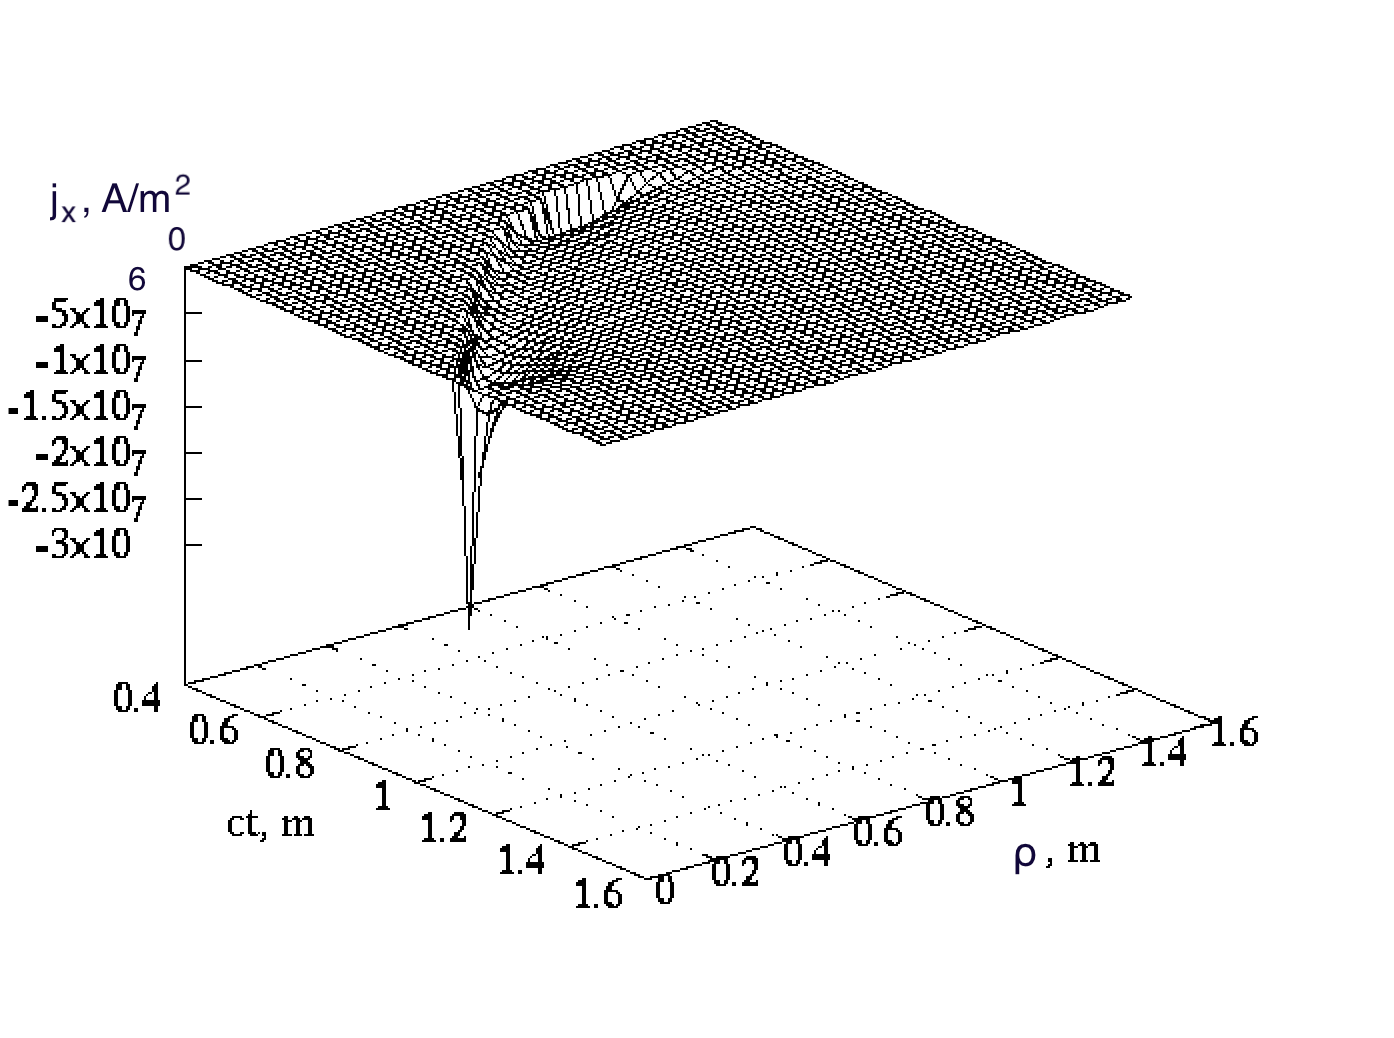
\includegraphics[scale=0.5]{Jperp_A1}
\caption{Нелінійність амплітуди вторинного джерела}
\label{fig:jx_secondary}
\end{center} \end{figure}

З виразів \eqref{eq:i1_partder}, \eqref{eq:i2_partder} очевидна нелінійна 
залежність струму від $ A_0 $.

%%%%%%%%%%%%%%%%%%%%%%%%%%%%%%%%%%%%%%%%%%%%%%%%%%%%%%%%%%%%%%%%%%%%%%%%%%%%%%%%
\section{Енергетичний розподіл поля плаского диску в лінійному наближенні}

Вторинний електричний струм розподілений в усьому напівпросторі $ z > 0 $,
але за рахунок згасання енергії з відстанню в межах $ [1/R, 1/R^2] $ (в 
залежності від напрямку спостереження) можемо обмежити область де треба 
враховувати нелінійні ефекти за рахунок високої концентрації енергії. Для 
визначення параметричних меж застосування введеної моделі нелінійності та 
оцінки границі зони, де нелінійні ефекти треба враховувати, розглянемо 
енергетичні характеристики поля в ближній зоні

Тепер розглянемо енергетичний розподіл від поля плаского диску при різних
часових залежностей $ f(t) $ стороннього струму. Побудова класичної 
енергетичної діаграми спрямованості мало інформативне дослідження нелінійних
ефектів - в даній роботі важливим є енергетичний розподіл в ближній зоні.

Розглянемо густину енергії електромагнітного поля $ \vect{E} $, збудженого 
пласким диском електричного струму з довільною часовою залежністю $ f(t) $ за 
визначенням \cite{imp:Schantz2018}, нехтуючи при цьому енергетичним внеском 
$ \vect{H} $ спираючись на відсутність нелінійного внеску останньої.

\begin{equation} \label{eq:energy}
W = \frac{\epsilon_0}{2} \int_0^\infty \vect{E}^2 dt
\end{equation}

Користуючись властивостями перехідної функції можемо обмежити
область інтегрування за часом, а також спростити підінтегральний вираз

\begin{equation} \label{eq:energy}
W = \frac{\epsilon_0}{2} \frac{\mu_0 \mu}{\epsilon_0 \epsilon}
\int_{ct_1}^{c\tau_0+ct_3} \left( E_\rho^2 + E_\varphi^2 \right) dt
\end{equation}

Також оцінено енергію перехідної функції, а тобто \ref{eq:energy} при 
часовій залежності сигналу у вигляді функції Гевісайда $ f(t) = H(t) $:

\textcolor{blue}{ \begin{equation*} \begin{aligned}
\vect{E}^2 = \frac{A_0^2}{4} \frac{\mu_0 \mu}{\epsilon_0 \epsilon}
\Big( I_1^2 \cos^2 \varphi + \left( I_2 - I_1 \right)^2 \sin^2 \varphi \Big)
\end{aligned} \end{equation*} }
%
\begin{equation} \label{eq:energy_tr}
W_{tr} = \frac{\epsilon_0 A_0^2}{8} \frac{\mu_0 \mu}{\epsilon_0 \epsilon}
\int_{ct_1}^{ct_3}  \Big( I_1^2 \cos^2 \varphi + 
\left( I_2 - I_1 \right)^2 \sin^2 \varphi \Big) dt.
\end{equation}

Розглядаючи особливий випадок \ref{eq:energy_tr} для $ \rho = 0 $, помічаємо,
що енергія випромінювання плаского диску, завжди лежить у наступних межах для 
сигналів з часовою залежністю $ f(t) $ з областю значень 
$ \left[ -1, 1 \right] $ та тривалістю $ \tau_0 $:

\textcolor{blue}{ \begin{equation*}
\left. W \right|^{\rho=0} = \frac{\epsilon_0 A_0^2}{32} 
\frac{\mu_0 \mu}{\epsilon_0 \epsilon} \Big( \sqrt{R^2+z^2} - z \Big)
\end{equation*} }
%
\textcolor{blue}{ \begin{equation*}
\int_{ct_1}^{c\tau_0+ct_3} 
\left( \int_0^t f(\tau) d \tau < \tau_0 \right) dt < \tau_0 R
\end{equation*} }
%
\begin{equation}
0 \leq W_{max} \left( \tau_0, f(t), \vect{r} \right) < 
\frac{\epsilon_0 \tau_0 R A_0^2}{32} \frac{\mu_0 \mu}{\epsilon_0 \epsilon},
\end{equation}
%
де $ W_{max} $ - густина енергії, $ \tau_0 $ - ефективна тривалість імпульсу 
за визначеною метрикою, $ A_0 $ - максимальна амплітуда сигналу, $ R $ - 
радіус апертури, а вираз під коренем - імпеданс у середовищі розповсюдження 
хвилі.

Будуватимемо поперечні зрізи значень енергій
для різних довжин імпульсів та для різних відстаней від джерела.
Для збереження кутового розміру зрізів візьмемо його $ z + 2R $.

\textcolor{red}{ TODO: побудувати поздовжні та поперечні енергетичні зрізи
для декількох $ f(t) $ }

\textcolor{red}{ Як видно з рисунків, форма збудження має значний вплив на 
розподіл енергії у ближній зоні, де вклад нелінійної поправки найбільший, а 
отже обмежувати область врахування вторинного струму на основі енергетичних 
характеристик породжувальної хвилі треба з урахуванням часової залежності 
струму }

\textcolor{red}{ TODO: можна строго порівняти діаграму спрямованості 
отриману в часовій області з діаграмою Баума, а також оцінити її відхилення 
в ближній зоні }

%%%%%%%%%%%%%%%%%%%%%%%%%%%%%%%%%%%%%%%%%%%%%%%%%%%%%%%%%%%%%%%%%%%%%%%%%%%%%%%%
\section{Модовий розподіл Керрівської поправки}

Застосуємо метод еволюційних рівнянь для розв'язання задачі випромінювання 
вторинним струмом \eqref{eq:j_kerr}. Для цього, спершу, запишемо модовий
розподіл джерела, який є правою частиною рівняння Клейна-Гордона. 

\textcolor{blue} { \begin{equation*}
j_m \left( r, t; \nu \right) = \frac{\sqrt{\mu_0}}{2\pi} 
\int \limits_{0}^{2\pi} d \varphi \int \limits_0^\infty \rho d \rho 
\vect{j_0} \crossprod{ \nabla_\perp \Psi_m^* }{ \vect{z_0} }
\end{equation*} }
%
\textcolor{blue} { \begin{equation*} 
\vect{J^\prime} = 
\vect{\rho_0}    \partder{}{t} P_\rho^\prime    \left( \vect{E} \right) + 
\vect{\varphi_0} \partder{}{t} P_\varphi^\prime \left( \vect{E} \right) + 
\vect{z_0}       \partder{}{t} P_z^\prime       \left( \vect{E} \right) 
\end{equation*} }
%
\textcolor{blue} { \begin{equation*} \begin{aligned}
\crossprod{ \nabla_\perp \Psi_m^* }{ \vect{z_0} } =
- \vect{\rho_0} i m e^{-im\varphi} \frac{J_m (\nu \rho)}{\rho \sqrt{\nu}}
- \vect{\varphi_0} \sqrt{\nu} e^{-im\varphi} 
\frac{J_{m-1} (\nu \rho) - J_{m+1} (\nu \rho)}{2}
\end{aligned} \end{equation*} }
%
\textcolor{blue} { \begin{equation*} \begin{aligned}
\vect{J^\prime} \crossprod{ \nabla_\perp \Psi_m^* }{ \vect{z_0} } = 
- i e^{-im\varphi} m \frac{J_m (\nu \rho)}{\rho \sqrt{\nu}}
\partder{}{t} P_\rho^\prime \left( \vect{E} \right) - \\
- \sqrt{\nu} e^{-im\varphi} \frac{J_{m-1} (\nu \rho) - J_{m+1} (\nu \rho)}{2}
\partder{}{t} P_\varphi^\prime \right)
\end{aligned} \end{equation*} }

\begin{equation*} \begin{aligned}
j_m = - \frac{\sqrt{\mu_0}}{2\pi} 
\int_{0}^{2\pi} d \varphi \int \limits_{0}^{\infty} \rho d \rho
e^{-im\varphi} \left( i  m \frac{J_m (\nu \rho)}{\rho \sqrt{\nu}}
\partder{j_\rho^\prime}{t} + \sqrt{\nu}
\frac{J_{m-1} (\nu \rho) - J_{m+1} (\nu \rho)}{2}
\partder{j_\varphi^\prime}{t} \right)
\end{aligned} \end{equation*}

Спершу, перейдемо від комплексної області визначення модового розподілу 
до уявної. Згрупувавши доданки за тригонометричними функціями,
знайдемо інтеграли за азимутальним кутом $ \varphi $, користуючись 
аналітичними інтегралами \eqref{eq:int_exp3}, \eqref{eq:int_exp4}, 
\eqref{eq:int_exp5}, \eqref{eq:int_exp6}. Отримаємо вирази для інтегралів
від компонентів вектору вторинного нелінійного струму з ядром інтегралу у 
вигляді комплексної експоненти.

\textcolor{blue} { \begin{equation*} \begin{aligned}
\int_0^{2\pi} e^{-i m \varphi} \cos^3 \varphi d \varphi = 
\frac{\pi}{4} \delta_{m,-3} + \frac{\pi}{4} \delta_{m,3} + 
\frac{3 \pi}{4} \delta_{m,-1} + \frac{3 \pi}{4} \delta_{m,1}
\end{aligned} \end{equation*} }
%
\textcolor{blue} { \begin{equation*} \begin{aligned}
\int_0^{2\pi} e^{-i m \varphi} \cos \varphi \sin^2 \varphi d \varphi = 
\frac{\pi \delta_{m,1} }{4} + \frac{\pi \delta_{m,-1} }{4} - 
\frac{\pi \delta_{m,-3} }{4} - \frac{\pi \delta_{m,3} }{4}
\end{aligned} \end{equation*} }
%
\textcolor{blue} { \begin{equation*} \begin{aligned}
\int_{0}^{2 \pi} d \varphi e^{-im \varphi} \partder{P_\rho^\prime}{t} = 
\frac{ {A_0}^3 \epsilon_0 \chi_e^{(3)} }{ 8 } \int_{0}^{2\pi} d \varphi
e^{-im\varphi} \left( \frac{\mu_0 \mu} {\epsilon_0 \epsilon} \right)^{3/2} 
\left( 3 {I_1}^2 \partder{I_1}{t} \cos^3 \varphi + \right. \\
+ \left. ( I_2 - I_1 ) \cos \varphi \sin^2 \varphi \left( 
\partder{I_1}{t} ( I_2 - I_1 ) + 2 I_1 \left( \partder{I_2}{t} - 
\partder{I_1}{t} \right) \right) \right) = \\
= \frac{ {A_0}^3 \epsilon_0 \chi_e^{(3)} }{ 8 } 
\left( \frac{\mu_0 \mu} {\epsilon_0 \epsilon} \right)^{3/2}
\left( \frac{3 \pi}{4} {I_1}^2 \partder{I_1}{t} \left( \delta_{m,-3} + 
\delta_{m,3} + 3 \delta_{m,-1} + 3 \delta_{m,1} \right) + \right. \\
+ \frac{\pi }{4} \left. ( I_2 - I_1 ) \left( \delta_{m,1} + 
\delta_{m,-1} - \delta_{m,-3} - \delta_{m,3} \right) \left( 
\partder{I_1}{t} ( I_2 - I_1 ) + 2 I_1 \left( \partder{I_2}{t} - 
\partder{I_1}{t} \right) \right) \right)
\end{aligned} \end{equation*} }
%
\begin{equation*} \begin{aligned}
\frac{\epsilon_0 \chi_e^{(3)}}{2 \pi} \int_{0}^{2\pi} d \varphi 
e^{-im \varphi} \partder{P_\rho^\prime}{t} = 
\frac{ {A_0}^3 \epsilon_0 \chi_e^{(3)}}{ 64 } 
\left( \frac{\mu_0 \mu} {\epsilon_0 \epsilon} \right)^{3/2} \cdot \\ 
\cdot \left( 3 {I_1}^2 \partder{I_1}{t} \left( \delta_{m,-3} + 
\delta_{m,3} + 3 \delta_{m,-1} + 3 \delta_{m,1} \right) + \right. \\
+ \left. ( I_2 - I_1 ) \left( \delta_{m,1} + \delta_{m,-1} - 
\delta_{m,-3} - \delta_{m,3} \right) \left( 
\partder{I_1}{t} ( I_2 - I_1 ) + 2 I_1 \left( \partder{I_2}{t} - 
\partder{I_1}{t} \right) \right) \right)
\end{aligned} \end{equation*}
%
\textcolor{blue} { \begin{equation*} \begin{aligned}
\int_{0}^{2\pi} e^{-i m \varphi} \sin^3 \varphi d \varphi = 
\frac{3 \pi i}{4} \delta_{m,-1} - \frac{3 \pi i}{4} \delta_{m,1} - 
\frac{\pi i}{4} \delta_{m,-3} + \frac{\pi i}{4} \delta_{m,3}
\end{aligned} \end{equation*} }
%
\textcolor{blue} { \begin{equation*} \begin{aligned}
\int_0^{2\pi} e^{-i m \varphi} \sin \varphi \cos^2 \varphi d \varphi = 
\frac{\pi i }{4} \delta_{m,-1} - \frac{\pi i }{4} \delta_{m,1} -
\frac{\pi i }{4} \delta_{m,3} + \frac{\pi i }{4} \delta_{m,-3}
\end{aligned} \end{equation*} }
%
\textcolor{blue} { \begin{equation*} \begin{aligned}
\int_{0}^{2 \pi} d \varphi e^{-im \varphi} \partder{P_\varphi^\prime}{t} = \\
= - \frac{ {A_0}^3 \epsilon_0 \chi_e^{(3)} }{ 8 } 
\int_{0}^{2 \pi} d \varphi e^{-im \varphi}
\left( \frac{\mu_0 \mu} {\epsilon_0 \epsilon} \right)^{3/2} \left(
3 ( I_2 - I_1 )^2 \left( \partder{I_2}{t} - \partder{I_1}{t} \right)
\sin^3 \varphi \right. + \\
+ \left. I_1 \sin \varphi \cos^2 \varphi \left( 
I_1 \left( \partder{I_2}{t} - \partder{I_1}{t} \right) + 
2 \partder{I_1}{t} (I_2 - I_1) \right) \right) = 
- \frac{ {A_0}^3 \epsilon_0 \chi_e^{(3)} }{ 8 } \cdot \\ 
\cdot \left( \frac{\mu_0 \mu} {\epsilon_0 \epsilon} \right)^{3/2} \left(
\frac{3 \pi i}{4} ( I_2 - I_1 )^2 \left( \partder{I_2}{t} - 
\partder{I_1}{t} \right) \left( 3 \delta_{m,-1} - 3 \delta_{m,1} - 
\delta_{m,-3} + \delta_{m,3} \right) \right. + \\
+ \left. \frac{\pi i}{4} I_1 \left( \delta_{m,-1} - \delta_{m,1} - 
\delta_{m,3} + \delta_{m,-3} \right) \left( 
I_1 \left( \partder{I_2}{t} - \partder{I_1}{t} \right) + 
2 \partder{I_1}{t} (I_2 - I_1) \right) \right)
\end{aligned} \end{equation*} }
%
\begin{equation*} \begin{aligned}
\frac{\epsilon_0 \chi_e^{(3)}}{2 \pi} \int_{0}^{2 \pi} d \varphi 
e^{-im \varphi} \partder{P_\varphi^\prime}{t} = 
- \frac{ {A_0}^3 \epsilon_0 \chi_e^{(3)}  i}{ 64 }
\left( \frac{\mu_0 \mu} {\epsilon_0 \epsilon} \right)^{3/2} \cdot \\ 
\cdot \left( 3 ( I_2 - I_1 )^2 \left( \partder{I_2}{t} - 
\partder{I_1}{t} \right) \left( 3 \delta_{m,-1} - 3 \delta_{m,1} - 
\delta_{m,-3} + \delta_{m,3} \right) \right. + \\
+ \left. I_1 \left( \delta_{m,-1} - \delta_{m,1} - 
\delta_{m,3} + \delta_{m,-3} \right) \left( 
I_1 \left( \partder{I_2}{t} - \partder{I_1}{t} \right) + 
2 \partder{I_1}{t} (I_2 - I_1) \right) \right)
\end{aligned} \end{equation*}

Як видно з останніх виразів, інтригування за кутом $ \varphi $ дає дискретний 
модовий розподіл вторинного струму.  Також помічаємо, що у розподілах присутні 
лише моді з номерами $ \pm 1 $ та $ \pm 3 $ - вклад вторинного струму в інші
моди відсутній. Випишемо окрему кожну з ненульових мод розподілу вторинного 
струму. Для цього введемо нові змінні:

\begin{equation} \begin{aligned} \label{eq:alpha}
\alpha = 3 {I_1}^2 \partder{I_1}{t}
\end{aligned} \end{equation}

\begin{equation} \begin{aligned} \label{eq:beta}
\beta = ( I_2 - I_1 ) \left( \partder{I_1}{t} ( I_2 - I_1 ) + 
2 I_1 \left( \partder{I_2}{t} - \partder{I_1}{t} \right) \right)
\end{aligned} \end{equation}

\begin{equation} \begin{aligned} \label{eq:gamma}
\gamma = 3 ( I_2 - I_1 )^2 \left( \partder{I_2}{t} - \partder{I_1}{t} \right)
\end{aligned} \end{equation}

\begin{equation} \begin{aligned} \label{eq:lambda}
\lambda = I_1^2 \left( \partder{I_2}{t} - 
\partder{I_1}{t} \right) + 2 I_1 \partder{I_1}{t} (I_2 - I_1)
\end{aligned} \end{equation}

Запишемо модовий розподіл струму через нові позначення, спростивши вираз 
можна отримати:

\textcolor{blue} { \begin{equation*} \begin{aligned}
j_m = - \frac{\sqrt{\mu_0}}{2\pi} 
\int_0^{2\pi} d \varphi \int \limits_0^\infty \rho d \rho
e^{-im\varphi} \left( i m \frac{J_m (\nu \rho)}{\rho \sqrt{\nu}}
j_\rho^\prime + \sqrt{\nu}
\frac{J_{m-1} (\nu \rho) - J_{m+1} (\nu \rho)}{2}
j_\varphi^\prime \right)
\end{aligned} \end{equation*} }
%
\textcolor{blue} { \begin{equation*} \begin{aligned}
j_m = - \frac{\sqrt{\mu_0}}{2\pi} 
\int_0^{2\pi} d \varphi \int \limits_0^\infty \rho d \rho 
e^{-im\varphi} \cdot \\ \cdot 
\left( i \sqrt{\nu} \frac{J_{m-1} (\nu \rho) + J_{m+1} (\nu \rho)}{2}
j_\rho^\prime + \sqrt{\nu} 
\frac{J_{m-1} (\nu \rho) - J_{m+1} (\nu \rho)}{2}
j_\varphi^\prime \right)
\end{aligned} \end{equation*} }
%
\textcolor{blue} { \begin{equation*} \begin{aligned}
j_m = - \frac{\sqrt{\mu_0} \sqrt{\nu}}{4\pi} 
\int_0^{2\pi} d \varphi \int \limits_0^\infty \rho d \rho 
e^{-im\varphi} \Big(
J_{m-1} (\nu \rho) ( i j_\rho^\prime + j_\varphi^\prime ) +
J_{m+1} (\nu \rho) ( i j_\rho^\prime - j_\varphi^\prime ) \Big)
\end{aligned} \end{equation*} }
%
\textcolor{red} { \begin{equation} \begin{aligned}
j_1 = \frac{i A_0^3 \sqrt{\mu_0} \epsilon_0 \chi_e^{(3)} \sqrt{\nu}}{128}
\left( \frac{\mu_0 \mu}{\epsilon_0 \epsilon} \right)^{3/2}
\int_0^\infty \rho d \rho \cdot \\ \cdot
\Big( J_0 (\nu \rho) ( 3 \alpha + \beta + 3 \gamma + \lambda) - J_2 (\nu \rho)
( 3 \alpha + \beta - 3 \gamma - \lambda ) \Big)
\end{aligned} \end{equation} }
%
\textcolor{blue} { \begin{equation*} \begin{aligned}
j_{-1} = \frac{i A_0^3 \sqrt{\mu_0} \epsilon_0 \chi_e^{(3)}}{64}
\left( \frac{\mu_0 \mu}{\epsilon_0 \epsilon} \right)^{3/2}
\int_0^\infty \rho d \rho \cdot \\ \cdot
\Big( \frac{J_1 (\nu \rho)}{\rho \sqrt{\nu}}
( 3 \alpha + \beta ) - \sqrt{\nu}
\frac{J_0 (\nu \rho) - J_2 (\nu \rho)}{2}
( 3 \gamma + \lambda ) \Big)
\end{aligned} \end{equation*} }
%
\textcolor{blue} { \begin{equation*} \begin{aligned}
j_{-1} = \frac{i A_0^3 \sqrt{\mu_0} \epsilon_0 \chi_e^{(3)} \sqrt{\nu}}{128}
\left( \frac{\mu_0 \mu}{\epsilon_0 \epsilon} \right)^{3/2}
\int_0^\infty \rho d \rho \cdot \\ \cdot
\Big( J_0 (\nu \rho) ( 3 \alpha + \beta - 3 \gamma - \lambda ) + 
J_2 (\nu \rho) ( 3 \alpha + \beta + 3 \gamma + \lambda ) \Big)
\end{aligned} \end{equation*} }
%
\textcolor{red} { \begin{equation} \begin{aligned}
j_{-1} = j_{1}
\end{aligned} \end{equation} }
%
\textcolor{red} { \begin{equation} \begin{aligned}
j_3 = \frac{i A_0^3 \sqrt{\mu_0} \epsilon_0 \chi_e^{(3)}}{64}
\left( \frac{\mu_0 \mu}{\epsilon_0 \epsilon} \right)^{3/2}
\int_0^\infty \rho d \rho \cdot \\ \cdot
\left( 3 m \frac{J_3 (\nu \rho)}{\rho \sqrt{\nu}}
( \alpha - \beta ) - \sqrt{\nu}
\frac{J_2 (\nu \rho) - J_4 (\nu \rho)}{2}
( \gamma - \lambda ) \right)
\end{aligned} \end{equation} }
%
\textcolor{blue} { \begin{equation*} \begin{aligned}
j_{-3} = - \frac{i A_0^3 \sqrt{\mu_0} \epsilon_0 \chi_e^{(3)}}{64}
\left( \frac{\mu_0 \mu}{\epsilon_0 \epsilon} \right)^{3/2}
\int_0^\infty \rho d \rho \cdot \\ \cdot
\left( 3 m \frac{J_3 (\nu \rho)}{\rho \sqrt{\nu}}
( \alpha - \beta ) - \sqrt{\nu}
\frac{J_2 (\nu \rho) - J_4 (\nu \rho)}{2}
( \gamma - \lambda ) \right)
\end{aligned} \end{equation*} }
%
\textcolor{blue} { \begin{equation*} \begin{aligned}
j_{-3} = - \frac{i A_0^3 \sqrt{\mu_0} \epsilon_0 \chi_e^{(3)} \sqrt{\nu}}{128}
\left( \frac{\mu_0 \mu}{\epsilon_0 \epsilon} \right)^{3/2}
\int_0^\infty \rho d \rho \cdot \\ \cdot
\Big( J_2 (\nu \rho) ( \alpha - \beta - \gamma + \lambda) + 
J_4 (\nu \rho) ( \alpha - \beta + \gamma - \lambda) \Big)
\end{aligned} \end{equation*} }
%
\textcolor{red} { \begin{equation} \begin{aligned}
j_{-3} = - j_{3}
\end{aligned} \end{equation} }

\textcolor{red}{ TODO: побудувати залежність $ j_m / vt $ від 
$ v^2t^2 - z^2 $ та $ \nu $ для всіх $ m $ у вигляді heatmaps. }

Для чисельного розрахунку невласного інтегралу по $ \rho $, що містяться в 
модових розподілах струму $ j_m $ зручно звузити межі інтегрування 
користуючись областю визначення під-інтегральної функцій $ S_2 $:

\textcolor{blue} { \begin{equation*} \begin{aligned}
(\rho - R)^2 \leq v^2t^2 - z^2 \leq (\rho + R)^2
\end{aligned} \end{equation*} }
%
\textcolor{blue} { \begin{equation*} \begin{aligned}
| \rho - R | - \sqrt{v^2t^2 - z^2} \leq 0 \leq \rho + R - \sqrt{v^2t^2 - z^2}
\end{aligned} \end{equation*} }
%
\textcolor{blue} { \begin{equation*} \begin{aligned}
- R - \sqrt{v^2t^2 - z^2} \leq - \rho \leq R - \sqrt{v^2t^2 - z^2}
\end{aligned} \end{equation*} }
%
\textcolor{blue} { \begin{equation*} \begin{aligned}
R + \sqrt{v^2t^2 - z^2} \geq \rho \geq - R + \sqrt{v^2t^2 - z^2}
\end{aligned} \end{equation*} }
%
\begin{equation} \begin{aligned}
\left| \sqrt{v^2t^2 - z^2} - R \right| \leq \rho \leq \sqrt{v^2t^2 - z^2} + R.
\end{aligned} \end{equation}

Задля відокремлення розмірних коефіцієнтів перевизначимо модовий розподіл 
струму:

\begin{equation} \begin{aligned}
j_m = - \frac{i A_0^3 \sqrt{\mu_0} \epsilon_0 \chi_e^{(3)} \sqrt{\nu}}{128}
\left( \frac{\mu_0 \mu}{\epsilon_0 \epsilon} \right)^{3/2} \hat{j_m}.
\end{aligned} \end{equation}

Так як поздовжня компонента вторинного струму $ J_z $ відсутня, рівняння 
Клейна-Гордона відносно поздовжнього електричного еволюційного коефіцієнту 
є однорідним, що згідно методом функції Рімана дає нульовий розв'язок для
цього коефіцієнту. Отже, як і у лінійному наближенні, електромагнітне поле 
з урахуванням ефектів слабкої нелінійності залишається ТЕ типу:

\textcolor{blue}{ \begin{equation*}
- \partial_{ct}(\mu I_n^e) - \partial_z V_n^e + \chi^2 e_n = 0
\end{equation*} }
%
\textcolor{blue}{ \begin{equation*}
\frac{\epsilon \mu}{ \sqrt{\epsilon_0 \mu_0}} 
\frac{\partial^2 e_n}{\partial t^2} - 
\frac{\partial^2 e_n}{\partial z^2} + \chi^2 e_n = 
- \frac{\sqrt{\mu_0}}{2 \pi c} 
\int_0^{2\pi} d \varphi 
\int_0^\infty \rho d \rho \Phi_n^* (\chi) \partder{J_z}{t} = 0
\end{equation*} }
%
\textcolor{blue}{ \begin{equation*}
e_n (z, t; \chi) = \iint_S j_n (t',z', \chi) G(t,t',z,z') dt' dz' = 0
\end{equation*} }
%
\textcolor{blue}{ \begin{equation*}
I_n^e = - \partial_{ct} (\epsilon e_n) - 
\frac{\sqrt{\mu_0}}{2 \pi} \int_0^{2\pi} d \varphi 
\int_0^{\infty} \rho d \rho \Phi_n^* (\chi) J_z
\end{equation*} }
%
\textcolor{blue}{ \begin{equation*}
\partial_{z} e_n = V_n^e
\end{equation*} }
%
\begin{equation} \label{eq:e_evolution}
e_n (z, t; \nu) = V_n^e (z, t; \nu) = I_n^e (z, t; \nu) = 0
\end{equation}

Пошук виразів для еволюційних коефіцієнтів починаємо з поздовжнього 
магнітного коефіцієнту $ h_m $. Для розглянутої фізичної моделі ізотропного
та стаціонарного середовища без втрат коефіцієнт $ h_m $ є розв'язком 
рівняння Клейна-Гордона. В лінійному випадку це рівняння містить електричну 
і магнітну сприйнятливості; для нелінійної нотації скористаємось поняттям 
ефективної сприйнятливості та методикою запропонованою R. Ziolkowski
\cite{imp:Ziolkowski1993}.

\begin{equation} \label{eq:klein_gordon_nl}
\frac{(\epsilon + \chi_e^{(3)}) \mu}{c^2} 
\frac{\partial^2 h_m}{\partial t^2} - 
\frac{\partial^2 h_m}{\partial z^2} + 
\nu^2 h_m = j_m (t',z'; \nu),
\end{equation}
%
де $ j_m (t',z'; \nu) $ - мода $ m $ дискретного розподілу стороннього 
джерела, $ \chi_e^{(3)} $ - відносна нелінійна електрична сприйнятливість 
середовища третього порядку, а величина $ \epsilon + \chi_e^{(3)} $ в 
літературі зустрічається, як ефективна нелінійна Керрівська сприйнятливість 
\cite{imp:Ziolkowski1993}. Тоді, розв'язком \eqref{eq:klein_gordon_nl} за 
методом функції Рімана буде \eqref{eq:klein_gordon_sol} з ядром у вигляді 
функції Рімана

\begin{equation*}
G(t,t',z,z') = \frac{v}{2} H \left( v (t-t') - (z-z') \right)
J_0 \left( \nu \sqrt{v^2 (t-t')^2 - (z-z')^2} \right),
\end{equation*}
%
де $ v $ - швидкість світла в середовищі з урахуванням нелінійного 
Керрівського сповільнення

\begin{equation}
v = \frac{c}{\sqrt{ \left(\epsilon + \chi_e^{(3)}\right) \mu}} = 
\left( \epsilon_0 
\left( \epsilon + \chi_e^{(3)} \right) \mu_0 \mu \right)^{-1/2}.
\end{equation}

Для отримання нелінійних поправок до напруженості електричного поля достатньо 
поперечного модового коефіцієнту $ V_m^h $, який лінійно залежить від $ h_m $

\textcolor{blue}{ \begin{equation*} 
h_m (z, t; \nu) = \iint_S j_m (t',z') G(t,t',z,z') dt' dz',
\end{equation*} }
%
\textcolor{blue}{ \begin{equation*}
V_m^h = - \mu \partial_{ct} (h_m)
\end{equation*} }
%
\textcolor{blue} { \begin{equation*} \begin{aligned} 
V_m^h = - \mu \partial_{ct} \int_0^\infty \int_0^\infty j_m (t',z') G dz' dt'
\end{aligned} \end{equation*} }
%
\textcolor{blue} { \begin{equation*} \begin{aligned} 
V_m^h = - \frac{v \mu}{2c}
\partder_{t} \int_0^\infty dz' \int_0^\infty 
dt' H \left( v (t-t') - (z-z') \right) \cdot \\
\cdot J_0 \left( \nu \sqrt{v^2 (t-t')^2 - (z-z')^2} \right) j_m (t',z')
\end{aligned} \end{equation*} }
%
\textcolor{blue} { \begin{equation*} \begin{aligned} 
V_m^h = - \frac{1}{2} \sqrt{\frac{\mu}{\epsilon + \chi_e^{(3)}}}
\partder_{t} \int_0^\infty dz' \int_0^\infty 
dt' H \left( v (t-t') - (z-z') \right) \cdot \\
\cdot J_0 \left( \nu \sqrt{v^2 (t-t')^2 - (z-z')^2} \right) j_m (t',z')
\end{aligned} \end{equation*} }
%
\textcolor{blue} { \begin{equation*} \begin{aligned} 
H \left( v (t-t') - z + z' \right) = 
H \left( - vt' - ( z - vt - z' ) \right) = \\
= H \left( vt' + ( z - vt - z' ) \right) = 
H \left( vt' - ( vt - z + z' ) \right)
\end{aligned} \end{equation*} }
%
\begin{equation} \begin{aligned} 
V_m^h = \frac{i A_0^3 \epsilon_0 \chi_e^{(3)}}{2^8}
\sqrt{\frac{\mu_0 \mu}{\epsilon + \chi_e^{(3)}}} 
\left( \frac{\mu_0 \mu}{\epsilon_0 \epsilon} \right)^{3/2} \sqrt{\nu} 
\cdot \\ \cdot \partder{}{t} \int_0^\infty dz' \int_0^{vt - z + z'} dt'
J_0 \left( \nu \sqrt{v(t-t')^2 - (z-z')^2} \right) \hat{j_m} (vt',z')
\end{aligned} \end{equation}

Тепер, користуючись правилом інтегрування Лейбніца, спростимо отриманий 
вираз взявши аналітично похідну за часом:
%
\textcolor{blue} { \begin{equation*} \begin{aligned}
\partder{}{\tau} 
J_0 \left( \nu \sqrt{\Delta \tau^2 - \Delta z^2} \right) = 
- \nu \Delta \tau 
\frac{J_1 \left( \nu \sqrt{\Delta \tau^2 - \Delta z^2} \right)}
{\sqrt{\Delta \tau^2 - \Delta z^2}}
\end{aligned} \end{equation*} }
%
\textcolor{blue} { \begin{equation*} \begin{aligned}
\partder{}{\theta} \int_{a(\theta)}^{b(\theta)} f(x,\theta) dx = 
\int_{a(\theta)}^{b(\theta)} \partder{f}{\theta} dx + 
f\big( b(\theta), \theta \big) \partder{b}{\theta} -
f\big( a(\theta), \theta \big) \partder{a}{\theta}
\end{aligned} \end{equation*} }
%
\textcolor{blue} { \begin{equation*} \begin{aligned}
\partder_{t} \int_0^{vt - z + z'} dt'
J_0 \left( \nu \sqrt{v(t-t')^2 - (z-z')^2} \right) \hat{j_m} (vt',z') = \\
= \int_0^{vt - z + z'} dvt' \partder{J_0}{vt} \hat{j_m} (vt',z') + \\
+ \left. 
J_0 \left( \nu \sqrt{v(t-t')^2 - (z-z')^2} \right) \hat{j_m} (vt',z')
\right|^{vt' = vt - z + z'}
\end{aligned} \end{equation*} }
%
\textcolor{blue} { \begin{equation*} \begin{aligned}
\left. v(t-t')^2 - (z-z')^2 \right|^{vt' = vt - z + z'} = 
vt^2 - (vt - z + z')^2 - (z-z')^2 = \\
= vt^2 - (vt - z)^2 + 2 z' (vt - z) + z'^2 - (z-z')^2 = \\
= 2 vt z - z^2 + 2 z' (vt - z) + z'^2 - z^2 + 2 z z' - z'^2 = \\
= 2 vt z - 2 z^2 + 2 z' (vt - z) + 2 z z' = 
2 \big( z (vt - z) + z' (vt - z) + z z' \big) = \\
2 \big( z (vt - z) + z' (vt - z + z) \big) = 
2 \big( z (vt - z) + vt z' \big) = \\
= 2 \big( vt z - z^2 + vt z' \big) = 2 vt (z + z') - 2 z^2
\end{aligned} \end{equation*} }
%
\textcolor{blue} { \begin{equation*} \begin{aligned}
\partder_{t} \int_0^{vt - z + z'} dt'
J_0 \left( \nu \sqrt{v(t-t')^2 - (z-z')^2} \right) \hat{j_m} (vt',z') = \\
= - \nu v (t-t') 
\frac{J_1 \left( \nu \sqrt{v(t-t')^2 - (z-z')^2} \right)}
{\sqrt{v(t-t')^2 - (z-z')^2}} + \\
+ J_0 \left( \nu \sqrt{2 vt (z + z') - 2 z^2} \right) 
\hat{j_m} (vt - z + z',z')
\end{aligned} \end{equation*} }
%
\begin{equation} \begin{aligned} \label{eq:vmh_nl}
V_m^h = \frac{i A_0^3 \epsilon_0 \chi_e^{(3)}}{2^8}
\sqrt{\frac{\mu_0 \mu}{\epsilon + \chi_e^{(3)}}} 
\left( \frac{\mu_0 \mu}{\epsilon_0 \epsilon} \right)^{3/2} \sqrt{\nu}
\int_0^\infty dz' \cdot \\ \cdot 
\left\{ J_0 \left( \nu \sqrt{2 vt (z + z') - 2 z^2} \right) 
\hat{j_m} (vt - z + z',z') - \right. \\ 
\left. - \nu \int_0^\infty v (t-t') 
\frac{J_1 \left( \nu \sqrt{v(t-t')^2 - (z-z')^2} \right)}
{\sqrt{v(t-t')^2 - (z-z')^2}} \hat{j_m} (vt',z') dt' \right\}
\end{aligned} \end{equation}

\begin{equation} \begin{aligned} \label{eq:vmh_norm}
V_m^h = \frac{i A_0^3 \epsilon_0 \chi_e^{(3)}}{2^8}
\sqrt{\frac{\mu_0 \mu}{\epsilon + \chi_e^{(3)}}} 
\left( \frac{\mu_0 \mu}{\epsilon_0 \epsilon} \right)^{3/2} 
\sqrt{\nu} \hat{V_m^h}
\end{aligned} \end{equation}

Як видно з \eqref{eq:vmh_nl}, властивості симетрії відносно номеру моди 
$ m $ у еволюційних коефіцієнтів зберігаються відносно модового розподілу 
струму, тому:

\begin{equation} \begin{aligned} \label{eq:vp1_vm1}
V_1^h = V_{-1}^h
\end{aligned} \end{equation}

\begin{equation} \begin{aligned} \label{eq:vp3_vm3}
V_3^h = - V_{-3}^h
\end{aligned} \end{equation}

\textcolor{red} { \begin{equation*} \begin{aligned}
\frac{J_1 \left( \nu \sqrt{\Delta \tau^2 - \Delta z^2} \right)}
{\nu \sqrt{\Delta \tau^2 - \Delta z^2}} =
\frac{J_0 \left( \nu \sqrt{\Delta \tau^2 - \Delta z^2} \right) +
J_2 \left( \nu \sqrt{\Delta \tau^2 - \Delta z^2} \right)}{2}
\end{aligned} \end{equation*} }


%%%%%%%%%%%%%%%%%%%%%%%%%%%%%%%%%%%%%%%%%%%%%%%%%%%%%%%%%%%%%%%%%%%%%%%%%%%%%%%%
\section{Числовий розрахунок нелінійної поправки}

Для розв'язання задачі випромінювання у вільний простір, згідно методу 
модового базису, необхідно підставити в розклад компонентів поля знайдені 
методом еволюційних рівнянь коефіцієнти. Як було доведено в 
\eqref{eq:e_evolution}, всі електричні еволюційні коефіцієнти нульові,
а отже за визначенням \textcolor{red}{[ТРЕТЯКОВ]} поздовжня електрична
компонента відсутня, як і у лінійному випадку:

\begin{equation} \label{eq:ez_kerr}
E'_z = \frac{1}{\sqrt{\epsilon_0}} \sum_{n=-\infty}^{\infty}
\int_0^\infty \chi^2 d \chi e_n (\nu | vt, z) \Phi_n (\nu | \rho, \phi) = 0,
\end{equation}
%
де $ \Phi_n $ - базисна функція розкладу \textcolor{red}{[ТРЕТЯКОВ]}.

З \eqref{eq:ez_kerr} пласка TE хвиля залишається TE при розповсюдженні 
крізь нелінійне середовище при слабких ефектах самодії, навіть при 
нестаціонарному збудженні.

Поперечні електричні компоненти поля, в свою чергу, визначені наступним 
розкладом \textcolor{red}{[ТРЕТЯКОВ]}:

\begin{equation} \begin{aligned}
\vect{E_\perp} = \frac{1}{\sqrt{\epsilon_0}} \left( 
\sum \limits_{m=-\infty}^{\infty} \int \limits_{0}^{\infty} 
d \nu V_m^h \crossprod{ \nabla_\perp \Psi_m }{ \vect{z_0} } +
\sum \limits_{n=-\infty}^{\infty} \int \limits_{0}^{\infty}
d \chi V_n^e \nabla_\perp \Phi_n \right),
\end{aligned} \end{equation}
%
де $ \Psi_m $ та $ \Phi_n  $ є базисні функції розкладу поля, а $ V_m^h $
та $ V_n^e $ - еволюційні коефіцієнти, відомі з виразів \eqref{eq:e_evolution}
та \eqref{eq:vmh_nl}. Користуючись властивостями симетрії мод 
\eqref{eq:vp1_vm1} та \eqref{eq:vp3_vm3}, не важко помітити, що

%
\textcolor{blue} { \begin{equation*} \begin{aligned}
\crossprod{ \nabla_\perp \Psi_m }{ \vect{z_0} } = 
- e^{im\varphi} \left( \vect{\varphi_0} \sqrt{\nu} 
\frac{J_{m-1} (\nu \rho) - J_{m+1} (\nu \rho)}{2} - 
i m \vect{\rho_0} \frac{J_m (\nu \rho)}{ \rho \sqrt{\nu}} \right)
\end{aligned} \end{equation*} }
%
\textcolor{blue} { \begin{equation*} \begin{aligned}
E'_\rho = \frac{1}{\sqrt{\epsilon_0}} \sum_{m=-\infty}^{\infty} 
i m e^{im\varphi} \int_{0}^{\infty} \frac{d \nu}{\sqrt{\nu}} 
V_m^h \frac{J_m(\nu \rho)}{\rho}
\end{aligned} \end{equation*} }

\textcolor{blue} { \begin{equation*} \begin{aligned}
\sum_{m=-\infty}^\infty m e^{im \varphi} V_m^h J_m(\nu \rho) = \\ =
  e^{  i \varphi} V_{ 1}^h J_{ 1}(\nu \rho) - 
  e^{- i \varphi} V_{-1}^h J_{-1}(\nu \rho) + \\ +
3 e^{ 3i \varphi} V_{ 3}^h J_{ 3}(\nu \rho) - 
3 e^{-3i \varphi} V_{-3}^h J_{-3}(\nu \rho) = \\ =
\left( e^{ i\varphi} + e^{- i\varphi} \right) V_1^h J_1(\nu \rho) + 
3 \left( e^{3i\varphi} + e^{-3i\varphi} \right) V_3^h J_3(\nu \rho) = \\
= 2 \cos \varphi V_1^h J_1(\nu \rho) + 
6 \cos 3 \varphi V_3^h J_3(\nu \rho)
\end{aligned} \end{equation*} }

\begin{equation} \begin{aligned}
E'_\rho = \frac{2 i \cos \varphi}{\sqrt{\epsilon_0}}
\int_0^\infty \sqrt{\nu} d \nu V_1^h \frac{J_1(\nu \rho)}{\nu \rho} +
\frac{6 i \cos 3 \varphi}{\sqrt{\epsilon_0}}
\int_0^\infty \sqrt{\nu} d \nu V_3^h \frac{J_3(\nu \rho)}{\nu \rho}.
\end{aligned} \end{equation}

Тепер, користуючись раніше введеним нормуванням еволюційного коефіцієнта 
\eqref{eq:vmh_norm} запишемо вираз для нелінійної поправки до напруженості 
електричного поля $ E'_\rho $ в зручному для порівняння з лінійним наближенням
\eqref{eq:linear_e_cyl} вигляді:

\textcolor{blue} { \begin{equation*} \begin{aligned}
E'_\rho = - \frac{A_0^3 \epsilon_0 \chi_e^{(3)}}{2^7}
\sqrt{\frac{\mu_0 \mu}{\epsilon_0 \left( \epsilon + \chi_e^{(3)} \right)}} 
\left( \frac{\mu_0 \mu}{\epsilon_0 \epsilon} \right)^{3/2} \cdot \\
\cdot \int_0^\infty \nu d \nu \left(
\cos \varphi \hat{V_1^h} \frac{J_1(\nu \rho)}{\nu \rho} +
3 \cos 3\varphi \hat{V_3^h} \frac{J_3(\nu \rho)}{\nu \rho} 
\right)
\end{aligned} \end{equation*} }

\textcolor{blue} { \begin{equation*} \begin{aligned}
\epsilon_0 \chi_e^{(3)}
\sqrt{\frac{\mu_0 \mu}{\epsilon_0 \left( \epsilon + \chi_e^{(3)} \right)}} 
\left( \frac{\mu_0 \mu}{\epsilon_0 \epsilon} \right)^{3/2} 
\frac{\sqrt{\epsilon}}{\sqrt{\epsilon}} =
\frac{\epsilon_0 \sqrt{\epsilon} \chi_e^{(3)}}
{\sqrt{\epsilon + \chi_e^{(3)}}} 
\left( \frac{\mu_0 \mu}{\epsilon_0 \epsilon} \right)^2
\end{aligned} \end{equation*} }
%
\textcolor{blue} { \begin{equation*} \begin{aligned}
\frac{\sqrt{\epsilon}}
{\sqrt{\epsilon + \chi_e^{(3)}}} =
\frac{\sqrt{\epsilon \mu}}{c} 
\frac{c}{\sqrt{\mu \left( \epsilon + \chi_e^{(3)} \right)}} = 
\frac{v_{NL}}{v_{LN}}
\end{aligned} \end{equation*} }

\begin{equation} \begin{aligned} \label{eq:erho_kerr}
E'_\rho = - \frac{\epsilon_0 \chi_e^{(3)} A_0^3}{2^7}
\frac{v_{NL}}{v_{LN}}
\left( \frac{\mu_0 \mu}{\epsilon_0 \epsilon} \right)^2
\left(\hat{E}_\rho^{(1)} \cos \varphi +
\hat{E}_\rho^{(3)} \cos 3 \varphi \right),
\end{aligned} \end{equation}
%
де відношення $ v_{NL} / v_{LN} < 1 $ є коефіцієнтом нелінійного 
сповільнення породженої вторинної хвилі $ \vect{E'} $, а 
$ \hat{E}_\rho^{(m)} $ - функція, подібна за змістом та значенням до 
інтегральних виразів $ I_1 $ та $ I_2 $ з розв'язку у наближенні
лінійного розповсюджування \eqref{eq:linear_e_cyl}:

\begin{equation} \begin{aligned} \label{eq:erho_norm}
\hat{E}_\rho^{(m)} = \hat{E}_\rho^{(m)} (vt,\rho,z) = 
\int_0^\infty \nu d \nu \frac{m J_m(\nu \rho)}{\nu \rho} 
\hat{V_m^h} (\nu | vt,\rho,z).
\end{aligned} \end{equation}

Також серед множників помічаємо імпеданс вільного простору 
$ (\mu_0 \mu) / (\epsilon_0 \epsilon) $, куб максимальної амплітуди 
нестаціонарного струму плаского диску $ A_0^3 $ та абсолютну нелінійну 
сприйнятливість $ \epsilon_0 \chi_e^{(3)} $.

\textcolor{red}{РИСУНОК, ЩО ІЛЮСТРУЄ АМПЛІТУДНИЙ ЕФЕКТ САМОДІЮ ПРИ ВАРІЦІЇ 
ЛІНІЙНОГО КОЕФІЦІЄНТУ ВІДБИТТЯ}

З виразу \eqref{eq:erho_kerr} добре видно один з проявів амплітудної
самодії електромагнітного випромінювання. Як видно з лінійного розв'язку
збільшення коефіцієнту заломлення середовища "розтягує" нестаціонарний 
імпульс. Самодія цього ефекту у нелінійному середовищі зменшує 
максимальну амплітуду поля-поправки в 
$ \sqrt{\epsilon} / \sqrt{\epsilon} \chi_e^{(3)} $  разів, що відповідає 
швидкості світла з урахуванням нелінійної сприйнятливості до швидкості 
світла в середовищі у лінійному наближення. Варто зазначити, що цей ефект 
мало-значущій та складає лише $ 0.01\% $ від поля поправки, а тому ним 
можна знехтувати в цьому випадку. Варто перевірити його внесок при сильній 
нелінійній самодії. Даний ефект можна сприймати, як поправку до імпедансу 
вільного простору при врахуванні нелінійної сприйнятливості третього порядку:

\begin{equation*} \begin{aligned}
\frac{v_{NL}}{v_{LN}}
\left( \frac{\mu_0 \mu}{\epsilon_0 \epsilon} \right)^2 = 
\sqrt{\frac{\mu_0 \mu}{\epsilon_0 \left( \epsilon + \chi_e^{(3)} \right)}}
\sqrt[3]{\frac{\mu_0 \mu}{\epsilon_0 \epsilon}} 
\end{aligned} \end{equation*}

Розв'язок відносно нелінійної поправки \eqref{eq:erho_kerr} містить кутову 
залежність та константні коефіцієнти в явному вигляді. Інші змінні, тобто
$ vt, \rho, z $ представлені в $ \hat{E}_\rho^{(m)} $, що в свою чергу
є невласним кратним інтегралом дійсної області значень:

\textcolor{blue} { \begin{equation*} \begin{aligned}
\hat{V_m^h} = \int_0^z dz' 
\left\{ J_0 \left( \nu \sqrt{2 vt (z + z') - 2 z^2} \right) 
\hat{j_m} (vt - z + z',z') - \right. \\ 
\left. - \nu \int_0^{vt - z + z'} dvt' v (t-t') 
\frac{J_1 \left( \nu \sqrt{v(t-t')^2 - (z-z')^2} \right)}
{\sqrt{v(t-t')^2 - (z-z')^2}} \hat{j_m} (vt',z')  \right\}
\end{aligned} \end{equation*} }

\textcolor{red} { \begin{equation*} \begin{aligned}
j_1 = \frac{i A_0^3 \sqrt{\mu_0} \epsilon_0 \chi_e^{(3)} \sqrt{\nu}}{128}
\left( \frac{\mu_0 \mu}{\epsilon_0 \epsilon} \right)^{3/2}
\int_0^\infty \rho d \rho \cdot \\ \cdot
\Big( J_0 (\nu \rho) ( 3 \alpha + \beta + 3 \gamma + \lambda) - J_2 (\nu \rho)
( 3 \alpha + \beta - 3 \gamma - \lambda ) \Big)
\end{aligned} \end{equation*} }

\begin{equation} \begin{aligned}
\hat{V_m^h} = \int_{0}^{\infty} dz'
\left\{ J_0 \left( \nu \sqrt{2 vt (z + z') - 2 z^2} \right) 
\int_{0}^{\infty} \rho' d \rho'
f (\rho',vt - z + z',z') - \right. \\ 
\left. - \nu \int_{0}^{\infty} dvt' v (t-t') 
\frac{J_1 \left( \nu \sqrt{v(t-t')^2 - (z-z')^2} \right)}
{\sqrt{v(t-t')^2 - (z-z')^2}} 
\int_{0}^{\infty} \rho' d\rho'
f (\rho',vt',z')  \right\},
\end{aligned} \end{equation}
%
де $ f ( \nu | vt', \rho', z') $ - лінійна комбінація функцій виду
$ I_\alpha I_\beta \partder{I_\alpha}{vt} $ введених раніше 
\eqref{eq:alpha} - \eqref{eq:lambda}, як $ \alpha, \beta, \gamma, \lambda $:

\textcolor{red} { \begin{equation} \begin{aligned}
f ( \nu | vt', \rho', z') = 
J_0 (\nu \rho') (3 \alpha + \beta + 3 \gamma + \lambda) - \\
- J_2 (\nu \rho') (3 \alpha + \beta - 3 \gamma - \lambda).
\end{aligned} \end{equation} }

Інтегрування за штрихованими змінними є виконнанням принципу суперпозиції 
відносно точкових джерел у вигляді яких можна представити плаский диск, та
визначені відповідно у межах $ 0 \leq \rho' \leq \rho $,
$ 0 \leq z' \leq z $ та $ 0 \leq t' \leq t $. Користуючись цим, а також 
областю визначення під-інтегральних функцій та принципом причинності функції 
Рімана $ v(t-t')-(z-z') > 0 $, можна обмежити область інтегрування в 
останньому виразі:

\begin{equation} \begin{aligned}
0 \leq vt' \leq vt - z + z';
\end{aligned} \end{equation}

\begin{equation} \begin{aligned}
0 \leq z' \leq \min(z,2R),
\end{aligned} \end{equation}
%
де верхня межа значень $ z' $ також обмежена за рахунок попереднього аналізу 
енергетичних властивостей випромінювання в ближній зоні. Також, для окремих 
інтегралів за змінними $ \rho' $ область інтегрування буде різною. Для 
інтегралу в першому доданку

\begin{equation} \begin{aligned}
\left| \sqrt{v^2t'^2 - z'^2} - R \right| \leq \rho' \leq 
\sqrt{v^2t'^2 - z'^2} + R,
\end{aligned} \end{equation}
%
а в другому при $ vt' = vt - z + z' $, відповідно:

\textcolor{blue} { \begin{equation*} \begin{aligned}
\left. v^2 t'^2 - z'^2 \right|^{vt' = vt - z + z'} = 
(vt - z + z')^2 - z'^2 = (vt - z)^2 + 2 z' (vt - z) = \\
(vt - z) (vt - z + 2 z') = (vt - z) (vt + z') + (vt - z) (z + z')
\end{aligned} \end{equation*} }

\begin{equation} \begin{aligned}
\left| \sqrt{(vt - z) (vt - z + 2 z')} - R \right| \leq \rho' \leq 
\sqrt{(vt - z) (vt - z + 2 z')} + R.
\end{aligned} \end{equation}

Аналітичний розрахунок нормованого еволюційного коефіцієнту $ \hat{V_m^h} $
є недоцільним та може виявитись взагалі неможливим, тому залишаються лише
чисельні квадратурні методи розв'язку, які дадуть гарну точність в випадку,
кратних визначених інтегралів. Зовнішнім інтегралом в \eqref{eq:erho_kerr} є 
інтеграл за неперервним спектральним параметром $ \nu $. На жаль, фізичного
обґрунтування для обмеження цієї області інтегрування немає, а отже,
доцільно розділити чисельне розв'язання на два етапи:

\begin{enumerate}
	\item Чисельний розрахунок еволюційного коефіцієнту $ \hat{V_m^h} $ 
	для деякої області значень по параметру $ \nu $;
	\item Аналіз частотних характеристик під-інтегральної функції за $ \nu $ 
	та обмеження області інтегрування на основі аналізу, що дозволить 
	розрахувати абсолютну похибку чисельного методу.
\end{enumerate}

Аналогічно можна знайти поправку до $ \varphi $ проекції вектору 
напруженості електричного поля:

\textcolor{blue} { \begin{equation*} \begin{aligned}
E_\varphi = - \frac{1}{2 \sqrt{\epsilon_0}} \sum_{m=-\infty}^{\infty} 
e^{im\varphi} \int_{0}^{\infty} \sqrt{\nu} d \nu 
V_m^h \left( J_{m-1} (\nu \rho) - J_{m+1} (\nu \rho) \right)
\end{aligned} \end{equation*} }

\textcolor{blue} { \begin{equation*} \begin{aligned}
\sum_{m=-\infty}^\infty e^{im \varphi}
V_m^h \left( J_{m-1} (\nu \rho) - J_{m+1} (\nu \rho) \right) = \\
e^{  i \varphi} V_{ 1}^h \left( J_0 (\nu \rho) - J_2 (\nu \rho) \right) +
e^{- i \varphi} V_{-1}^h \left( J_2 (\nu \rho) - J_0 (\nu \rho) \right) + \\
e^{ 3i \varphi} V_{ 3}^h \left( J_2 (\nu \rho) - J_4 (\nu \rho) \right) +
e^{-3i \varphi} V_{-3}^h \left( J_4 (\nu \rho) - J_2 (\nu \rho) \right) = \\
= \left( e^{  i \varphi} - e^{- i \varphi} \right)
\left( J_0 (\nu \rho) - J_2 (\nu \rho) \right) +
\left( e^{ 3i \varphi} - e^{-3i \varphi} \right) 
\left( J_2 (\nu \rho) - J_4 (\nu \rho) \right) = \\
= 2i \sin \varphi \left( J_0 (\nu \rho) - J_2 (\nu \rho) \right) +
2i \sin 3 \varphi \left( J_2 (\nu \rho) - J_4 (\nu \rho) \right)
\end{aligned} \end{equation*} }

\textcolor{blue} { \begin{equation*} \begin{aligned}
E_\varphi =
- \frac{i \sin \varphi}{\sqrt{\epsilon_0}} \int_0^\infty d \nu
\sqrt{\nu} V_1^h \left( J_0 (\nu \rho) - J_2 (\nu \rho) \right) - \\
- \frac{i \sin 3 \varphi}{\sqrt{\epsilon_0}} \int_0^\infty d \nu
\sqrt{\nu} V_3^h \left( J_2 (\nu \rho) - J_4 (\nu \rho) \right)
\end{aligned} \end{equation*} }

\begin{equation} \begin{aligned} \label{eq:ephi_kerr}
E'_\varphi = \frac{\epsilon_0 \chi_e^{(3)} A_0^3}{2^7}
\frac{v_{NL}}{v_{LN}}
\left( \frac{\mu_0 \mu}{\epsilon_0 \epsilon} \right)^2
\left(\hat{E}_\varphi^{(1)} \sin \varphi +
\hat{E}_\varphi^{(3)} \sin 3 \varphi \right)
\end{aligned} \end{equation}
%
де 

\begin{equation} \begin{aligned} \label{eq:ephi_norm}
\hat{E}_\varphi^{(m)} (vt, \rho, z) = 
\int_0^\infty \nu d \nu V_m^h (\nu | vt, \rho, z)
\left( J_{m-1} (\nu \rho) - J_{m+1} (\nu \rho) \right)
\end{aligned} \end{equation}

В виразах \eqref{eq:erho_kerr} та \eqref{eq:ephi_kerr} спостерігається
утворення поля з тригонометричною кутовою залежністю кратних порядків.
Схожий ефект спостерігається, також, в задачах розповсюджування пласкої 
хвилі в частотних характеристиках при гармонійних часових залежностях.


Для аналізу та порівняння з лінійним розв'язком, зручно перейти до 
декартових проекцій вектору напруженості, тоді

\textcolor{blue} { \begin{equation*} \begin{aligned}
E'_x = E'_\rho \cos \varphi - E'_\varphi \sin \varphi
\end{aligned} \end{equation*} }
%
\textcolor{blue} { \begin{equation*} \begin{aligned}
E'_x = - \frac{\epsilon_0 \chi_e^{(3)} A_0^3}{2^7} \frac{v_{NL}}{v_{LN}}
\left( \frac{\mu_0 \mu}{\epsilon_0 \epsilon} \right)^2 \cdot \\ \cdot
\left(\hat{E}_\rho^{(1)} \cos^2 \varphi +
\hat{E}_\rho^{(3)} \cos \varphi \cos 3 \varphi - 
\hat{E}_\varphi^{(1)} \sin^2 \varphi -
\hat{E}_\varphi^{(3)} \sin \varphi \sin 3 \varphi \right)
\end{aligned} \end{equation*} }
%
\textcolor{blue} { \begin{equation*} \begin{aligned}
E'_x = - \frac{\epsilon_0 \chi_e^{(3)} A_0^3}{2^7} \frac{v_{NL}}{v_{LN}}
\left( \frac{\mu_0 \mu}{\epsilon_0 \epsilon} \right)^2 \cdot \\ \cdot
\int_0^\infty \nu d \nu V_1^h \left( 
\left( J_0 (\nu \rho) + J_2 (\nu \rho) \right) \cos^2 \varphi -
\left( J_0 (\nu \rho) - J_2 (\nu \rho) \right) \sin^2 \varphi \right) - \\
- \frac{\epsilon_0 \chi_e^{(3)} A_0^3}{2^7} \frac{v_{NL}}{v_{LN}}
\left( \frac{\mu_0 \mu}{\epsilon_0 \epsilon} \right)^2 \cdot \\ \cdot
\int_0^\infty \nu d \nu V_3^h \left( 
\left( J_2 (\nu \rho) + J_4 (\nu \rho) \right) \cos \varphi \cos 3 \varphi -
\left( J_2 (\nu \rho) - J_4 (\nu \rho) \right) \sin \varphi \sin 3 \varphi 
\right)
\end{aligned} \end{equation*} }

\textcolor{red} {TODO: ефект відставання та сповільнення хвилі}

\textcolor{red} {TODO: ефект самофокусування за рахунок залежності від кута}

%%%%%%%%%%%%%%%%%%%%%%%%%%%%%%%%%%%%%%%%%%%%%%%%%%%%%%%%%%%%%%%%%%%%%%%%%%%%%%%%
\section{Розповсюдження прямокутного імпульсу в нелінійному середовищі}

\textcolor{red} {TODO: Порушення закону збереження та принципу суперпозиції}

\textcolor{red} {TODO: Може вдається якось виділити залежність від 
тривалості імпульсу аналітично???}

%%%%%%%%%%%%%%%%%%%%%%%%%%%%%%%%%%%%%%%%%%%%%%%%%%%%%%%%%%%%%%%%%%%%%%%%%%%%%%%%
\section{Узагальнення для слабкої нелінійності}

Опираючись на геометрію джерела та на властивості модового базису можна 
довести, що 

\textcolor{red} { \begin{equation} \begin{aligned} \label{eq:erho_norm}
\hat{E}_\rho^{(1)} = \int_0^\infty \nu d \nu 
\frac{J_1(\nu \rho)}{\nu \rho} \hat{V_1^h} \approx
\int_0^\infty \nu d \nu \frac{J_1(\nu \rho)}{\nu \rho} 
\frac{J_1(\nu R) J_0(\nu \sqrt{v^2t^2-z^2})}{\nu} = I_1,
\end{aligned} \end{equation} }
%
отже компонент з лінійною залежністю від кута, повторює за формою 
імпульс отриманий у лінійному наближенні та менший за амплітудою на 
декілька порядків, а отже його внеском можна знехтувати.

\begin{equation*} \begin{aligned}
\lim_{n \to \infty} 
\sqrt{ \frac{\epsilon}{ \epsilon + \chi_e^{(2n+1)}} } = 1
\end{aligned} \end{equation*}

\textcolor{blue} { \begin{equation*} \begin{aligned}
E'_\rho = - \frac{\epsilon_0 \chi_e^{(3)} A_0^3}{2^7}
\frac{v_{NL}}{v_{LN}}
\left( \frac{\mu_0 \mu}{\epsilon_0 \epsilon} \right)^2
\left(\hat{E}_\rho^{(1)} \cos \varphi +
\hat{E}_\rho^{(3)} \cos 3 \varphi \right)
\end{aligned} \end{equation*} }

\textcolor{blue} { \begin{equation*} \begin{aligned}
E'_\rho = - \frac{\epsilon_0 \chi_e^{(3)} A_0^3}{2^7}
\frac{v_{NL}}{v_{LN}}
\left( \frac{\mu_0 \mu}{\epsilon_0 \epsilon} \right)^2 
\hat{E}_\rho^{(3)} \cos 3 \varphi
\end{aligned} \end{equation*} }

\begin{equation*} \begin{aligned}
E'_\rho = - \frac{1}{2} \sum_{n=1}^{\infty} 
\frac{\epsilon_0 \chi_e^{(2n+1)} A_0^{2n+1} }{ 4^{2n+1} }
\left( \frac{\mu_0 \mu}{\epsilon_0 \epsilon} \right)^{n+1}
\hat{E}_\rho^{(2n+1)} \cos (2n + 1) \varphi
\end{aligned} \end{equation*}

% \begin{tabular}{ | l | l | }
% \hline 
% Призначення змінної                          & Область визначенням       \\ 
% \hline
% Відстань, що проходить сигнал за час $t$     & $ 0 \le vt' \le vt $      \\ 
% \hline
% Відстань, від точки спостереження до джерела & $ 0 \le z' \le z $        \\  
% \hline
% Принцип причинності для проміжних подій      & $ 0 < vt - vt' - z + z' $ \\ 
% \hline
% Наслідок з 3 та 1                            & $ 0 < vt' < vt - z + z' $ \\ 
% \hline
% \end{tabular}

\chapter{Передача інформації через нелінійний простір}
\label{ch:neuron}

%%%%%%%%%%%%%%%%%%%%%%%%%%%%%%%%%%%%%%%%%%%%%%%%%%%%%%%%%%%%%%%%%%%%%%%%%%%%%%%
\section{Вплив нелінійності на імпульсний сигнал}

%%%%%%%%%%%%%%%%%%%%%%%%%%%%%%%%%%%%%%%%%%%%%%%%%%%%%%%%%%%%%%%%%%%%%%%%%%%%%%%
\section{Основні засоби підвищення кількості переданої інформації}

%%%%%%%%%%%%%%%%%%%%%%%%%%%%%%%%%%%%%%%%%%%%%%%%%%%%%%%%%%%%%%%%%%%%%%%%%%%%%%%
\section{Детекція сигналу за допомогою штучного інтелекту}

Процес передачі інформації в закодованому виді можна поділити на два етапи:
задача випромінювання та задача прийому. При використанні надширокосмугових 
протоколів канального рівня, станом на сьогодні, задача випромінювання вирішується 
ефективно. Задача прийому, в свою чергу, гальмується за рахунок 

%%%%%%%%%%%%%%%%%%%%%%%%%%%%%%%%%%%%%%%%%%%%%%%%%%%%%%%%%%%%%%%%%%%%%%%%%%%%%%%
\section{Задача визначення кута за формую імпульсу}

%%%%%%%%%%%%%%%%%%%%%%%%%%%%%%%%%%%%%%%%%%%%%%%%%%%%%%%%%%%%%%%%%%%%%%%%%%%%%%%
\section{Задача классифікації імпульсу в лінійному просторі}

%%%%%%%%%%%%%%%%%%%%%%%%%%%%%%%%%%%%%%%%%%%%%%%%%%%%%%%%%%%%%%%%%%%%%%%%%%%%%%%
\section{Задача классифікації імпульсу в нелінійному просторі}

%%%%%%%%%%%%%%%%%%%%%%%%%%%%%%%%%%%%%%%%%%%%%%%%%%%%%%%%%%%%%%%%%%%%%%%%%%%%%%%
\section{Задача клвсифікації в умовах детермінованого шуму}

%%%%%%%%%%%%%%%%%%%%%%%%%%%%%%%%%%%%%%%%%%%%%%%%%%%%%%%%%%%%%%%%%%%%%%%%%%%%%%%
\section{Нілінійність, як засіб підвищення кількості переданої інформації}

%\section{Методологія написання коду та вимоги до програмного продукту}
%\section{Програмний дизаін та архітектура коду}
%\section{Тестування програмного забеспечення та вілідація чисельних розв'язків}
%section{Чисельні методи розрахунку імпульсних полів}
%\section{Імпульсна антенна, як копмонент мереживного обряднання компьютера}


\chapter*{Висновки}

\begin{enumerate}

\item Побудовано аналітичне розв'язання у вигляді кусково визначеної функції для 
задачі випромінювання круглої апертури при нестаціонарному збуджені у вигляді 
прямокутної функції. Розв'язок отримано без наближення дальньої зони та визначено 
для всіх точок спостереження в кожен момент часу. Використання моделі круглої 
апертури, як моделі антен типу LIRA, перевірено на експериментальних даних в 
окремих точках та на даних, отриманих методом FDTD з комерційного 
електромагнітного симулятора CST Studio.

\item Отримане розв'язання задачі випромінювання плаского диску при збуджені у 
вигляді функції Хевісайда в лінійному наближенні має чітку просторово-часову 
зональність та ілюструє твердження Фарадея, що випромінює не антена, а простір 
довкола неї. Отримані області випромінювання наступають послідовно для довільної 
точки спостереження. Остання за часом настання область $ S_3 $ відповідає 
стаціонарному (усталеному) процесу випромінювання, коли всі точки апертури 
поєднані зі спостерігачем за принципом причинності. Настанню усталеного процесу 
передує область деякого транзитивного процесу $ S_2 $, поки поле від всієї 
апертури не досягне спостерігача. Найпершою для спостерігача просторово-часовою 
областю випромінювання в прожекторній зоні круглої апертури настає область 
електромагнітного снаряду $ S_1 $, де з хвилі у ТЕМ рупора формується ТЕ хвиля 
у вільному просторі.

\item При урахуванні нелінійних ефектів самодії у керрівському середовищі, 
квазі-плаский фронт хвилі, що формується пласким диском електричного струму, 
за своєю формою наближається до сферичного. При цьому, тип хвилі зберігається і
хвиля з урахуванням нелінійних ефектів залишається поперечною електричною (ТЕ). 

\item Нейронне радіо дозволяє на практиці реалізувати максимальний теоретичний
потенціал імпульсних надширокосмугових радіосистем у всіх областях застосування:
радіолокації, телекомунікації, зондування і тд. Головними перевагами таких систем 
в порівнянні з класичними є енергоефективність, а також якість розв'язання задач 
sequence-to-label і sequence-to-sequence за рахунок гнучкості системи.
Даний винахід розширює область застосування імпульсного радіо за 
рахунок покращених робочих характеристик. Підвищена стійкість до 
шуму дозволяє вирішувати радарні та телекомунікаційні задачі на 
більших відстанях. Можливість розпізнавати імпульси різної форми 
збудження уможливлює кодування корисного сигналу імпульсами різної форми, 
що підвищує швидкість передачі даних. 

\end{enumerate}

%\begin{bibset}{Список використаних джерел}
\bibliographystyle{acm}
% Для сортування літератури за алфавітом використовуйте
%\bibliographystyle{gost71s}
\bibliography{../my,../import}
%\end{bibset}
%GATHER{xampl-mybib.bib}

%\begin{bibset}[a]{Список публікацій автора}
%\bibliographystyle{acm}
%\bibliography{mybib}
%\end{bibset}


\appendix
\chapter{Дякі властивості тригонометричних функції}
\label{ch:trigonometric}

\textcolor{blue}{
\begin{equation*}
\derivat{}{\varphi} \arccos \varphi = - \frac{1}{ \sqrt{1 - \varphi^2} }
\end{equation*}
%
\begin{equation*}
\derivat{}{\varphi} \arctan \varphi = \frac{1}{1 + \varphi^2}
\end{equation*}
%
\begin{equation*}
\cos \alpha \cos \beta = \frac{1}{2} 
\left(  \cos (\alpha + \beta) + \cos (\alpha - \beta) \right)
\end{equation*}
%
\begin{equation*}
\sin \alpha \cos \beta = \frac{1}{2} 
\left( \sin (\alpha + \beta) + \sin (\alpha - \beta) \right)
\end{equation*}
%
\begin{equation*}
\sin \alpha \sin \beta = \frac{1}{2} 
\left( \cos (\alpha - \beta) - \cos (\alpha + \beta) \right)
\end{equation*}
%
\begin{equation*}
e^{im \varphi} = \cos m \varphi + i \sin m \varphi
\end{equation*}
%
\begin{equation*}
e^{-im \varphi} = \cos m \varphi - i \sin m \varphi
\end{equation*}
%
\begin{equation*}
\sin \varphi = \frac{e^{i \varphi} - e^{- i \varphi}}{2i}
\end{equation*}
%
\begin{equation*}
\cos \varphi = \frac{e^{i \varphi} + e^{- i \varphi}}{2}
\end{equation*}
%
\begin{equation*}
\arctan \frac{1}{x} = \frac{\pi}{2} - \arctan x
\end{equation*}
%
\begin{equation*}
\pi - \arccos x = \arccos (-x)
\end{equation*}
} % textcolor blue
%
\begin{equation}
\arccos x - \arccos y = \mp \arccos \left( 
xy + \sqrt{(1-x^2)(1-y^2)} \right),
\left\{ \begin{array}{c} x \ge y \\ x < y  \end{array} \right\}
\end{equation}
%
\begin{equation}
\arctan x - \arctan y = 
\arctan \frac{x-y}{1+xy}, xy > -1 
\end{equation}
%
\begin{equation}
\arctan x - \arctan y = \pm \pi + \arctan \frac{x-y}{1+xy}, 
\left\{ \begin{array}{c} x > 0 \\ x < 0  \end{array} \right\}, xy < -1 
\end{equation}

\section{Визначення дельта-функції, через інтеграли}
%
\begin{equation} \begin{aligned} \label{eq:int_exp0}
\int_{0}^{2\pi} e^{\pm i (m-n) \varphi} d \varphi = 2 \pi \delta_{m,n} 
\end{aligned} \end{equation}
%
\begin{equation} \begin{aligned} \label{eq:int_exp1}
\int \limits_{0}^{2\pi} d \varphi \sin \varphi 
\left( \cos m \varphi - i \sin m \varphi \right) = 
i \pi \left( \delta_{m,-1} - \delta_{m,1} \right)
\end{aligned} \end{equation}
%
\textcolor{blue}{ \begin{equation*} \begin{aligned}
\int_{0}^{2\pi} d \varphi \sin \varphi 
\left( \cos m \varphi - i \sin m \varphi \right) = \int_{0}^{2\pi} d \varphi
\left( \sin \varphi \cos m \varphi - i \sin \varphi \sin m \varphi \right) = \\
= \frac{1}{2} \int_{0}^{2\pi} d \varphi \left( \sin (\varphi + m \varphi) + 
\sin (\varphi - m \varphi) - i \cos (\varphi - m \varphi) + 
i \cos (\varphi + m \varphi) \right) = \\
= \frac{i}{2} \int_{0}^{2\pi} d \varphi \left( -i \sin (\varphi + m \varphi) -
i \sin (\varphi - m \varphi) - \cos (\varphi - m \varphi) + 
\cos (\varphi + m \varphi) \right) = \\
= \frac{i}{2} \int_{0}^{2\pi} d \varphi \left( e^{-i (\varphi + m \varphi)} - 
e^{i (\varphi - m \varphi)} \right) = 
i \pi \left( \delta_{m,-1} - \delta_{m,1} \right)
\end{aligned} \end{equation*} }
%
\begin{equation} \begin{aligned} \label{eq:int_exp2}
\int \limits_{0}^{2\pi} d \varphi \cos \varphi 
( \cos m \varphi - i \sin m \varphi) = \pi ( \delta_{m,-1} + \delta_{m,1} )
\end{aligned} \end{equation}
%
\textcolor{blue}{ \begin{equation*} \begin{aligned}
\int_{0}^{2\pi} d \varphi \cos \varphi 
\left( \cos m \varphi - i \sin m \varphi \right) = \int_{0}^{2\pi} d \varphi
\left( \cos \varphi \cos m \varphi - i \cos \varphi \sin m \varphi \right) = \\
= \frac{1}{2} \int_{0}^{2\pi} d \varphi \left( 
\cos (\varphi + m \varphi) + \cos (\varphi - m \varphi) - 
i \sin (m \varphi + \varphi) - i \sin (m \varphi - \varphi) \right) = \\
= \frac{1}{2} \int_{0}^{2\pi} d \varphi \left( 
\cos (\varphi + m \varphi) + \cos (\varphi - m \varphi) - 
i \sin (m \varphi + \varphi) + i \sin (\varphi - m \varphi) \right) = \\
= \frac{1}{2} \int_{0}^{2\pi} d \varphi 
\left( e^{-i (1 + m) \varphi} - e^{i (1 - m) \varphi} \right) = 
\pi \left( \delta_{m,-1} + \delta_{m,1} \right)
\end{aligned} \end{equation*} }
%
\begin{equation} \begin{aligned} \label{eq:int_exp3}
\int_0^{2\pi} e^{-i m \varphi} \cos \varphi \sin^2 \varphi d \varphi = 
\frac{\pi \delta_{m,1} }{4} + \frac{\pi \delta_{m,-1} }{4} - 
\frac{\pi \delta_{m,-3} }{4} - \frac{\pi \delta_{m,3} }{4}
\end{aligned} \end{equation}
%
\textcolor{blue}{ \begin{equation*} \begin{aligned}
e^{-i m \varphi} \cos \varphi \sin^2 \varphi = e^{-i m \varphi} 
\frac{e^{i\varphi} + e^{-i\varphi}}{2} \frac{1 - \cos 2\varphi}{2} = \\
\frac{2e^{-i(m-1)\varphi} + 2e^{-i(m+1)\varphi}}{8} - 
\frac{e^{2i\varphi} + e^{-2i\varphi}}{2} 
\frac{2e^{-i(m-1)\varphi} + 2e^{-i(m+1)\varphi}}{8} = \\
\frac{2e^{-i(m-1)\varphi} + 2e^{-i(m+1)\varphi}}{8} - 
\frac{e^{-i(m-3)\varphi} + e^{-i(m+1)\varphi} + 
e^{-i(m-1)\varphi} + e^{-i(m+3)\varphi}}{8} = \\
= \frac{e^{-i(m-1)\varphi}}{8} + \frac{e^{-i(m+1)\varphi}}{8} -
\frac{e^{-i(m-3)\varphi}}{8} - \frac{e^{-i(m+3)\varphi}}{8}
\end{aligned} \end{equation*} }
%
\begin{equation} \begin{aligned} \label{eq:int_exp4}
\int_{0}^{2\pi} e^{-i m \varphi} \sin^3 \varphi d \varphi = 
\frac{3 \pi i}{4} \delta_{m,-1} - \frac{3 \pi i}{4} \delta_{m,1} - 
\frac{\pi i}{4} \delta_{m,-3} + \frac{\pi i}{4} \delta_{m,3}
\end{aligned} \end{equation}
%
\textcolor{blue}{ \begin{equation*} \begin{aligned}
e^{-i m \varphi} \sin^3 \varphi = e^{-i m \varphi} 
\frac{1 - \cos 2\varphi}{2} \frac{e^{i\varphi} - e^{-i\varphi}}{2i} = \\
= \frac{e^{-i(m-1)\varphi} - e^{-i(m+1)\varphi}}{4i} - 
\frac{e^{-i(m-3)\varphi} + e^{-i(m+1)\varphi} -
e^{-i(m-1)\varphi} - e^{-i(m+3)\varphi}}{8i} = \\
= \frac{3 e^{-i(m-1)\varphi}}{8i} - \frac{3 e^{-i(m+1)\varphi}}{8i} - 
\frac{e^{-i(m-3)\varphi}}{8i} + \frac{e^{-i(m+3)\varphi}}{8i} = \\
= \frac{3i e^{-i(m+1)\varphi}}{8} - \frac{3i e^{-i(m-1)\varphi}}{8} + 
\frac{i e^{-i(m-3)\varphi}}{8} - \frac{i e^{-i(m+3)\varphi}}{8} 
\end{aligned} \end{equation*} }
%
\textcolor{blue}{ \begin{equation*} \begin{aligned}
\int_{0}^{2\pi} e^{-i m \varphi} \sin^3 \varphi d \varphi = 
\frac{i\pi}{4} \left( 3 \delta_{m,-1} - 3 \delta_{m,1} + 
\delta_{m,3} - \delta_{m,-3} \right)
\end{aligned} \end{equation*} }
%
\begin{equation} \begin{aligned} \label{eq:int_exp5}
\int_0^{2\pi} e^{-i m \varphi} \sin \varphi \cos^2 \varphi d \varphi = 
\frac{\pi i }{4} \delta_{m,-1} - \frac{\pi i }{4} \delta_{m,1} -
\frac{\pi i }{4} \delta_{m,3} + \frac{\pi i }{4} \delta_{m,-3}
\end{aligned} \end{equation}
%
\textcolor{blue}{ \begin{equation*} \begin{aligned}
e^{-i m \varphi} \sin \varphi \cos^2 \varphi = 
\cos^2 \varphi e^{-i m \varphi} \frac{e^{i\varphi} - e^{-i\varphi}}{2i} = \\
= \frac{1 + \cos 2\varphi}{2} 
\frac{e^{i(1-m)\varphi} - e^{-i(1+m)\varphi}}{2i} = \\
= \frac{e^{i(1-m)\varphi} - e^{-i(1+m)\varphi}}{4i} + 
\frac{e^{2i\varphi} + e^{-2i\varphi}}{2} 
\frac{e^{i(1-m)\varphi} - e^{-i(1+m)\varphi}}{4i} = \\
\frac{ 2 e^{i(1-m)\varphi} - 2 e^{-i(1+m)\varphi}}{8i} +
\frac{e^{i(3-m)\varphi} + e^{-i(1+m)\varphi} - 
e^{-i(m-1)\varphi} - e^{-i(3+m)\varphi}}{8i} = \\
= -\frac{ i e^{-i (m-1) \varphi} }{8} + \frac{ i e^{-i (m+1) \varphi} }{8} -
\frac{ i e^{-i (m-3) \varphi} }{8} + \frac{ i e^{-i (m+3) \varphi} }{8}
\end{aligned} \end{equation*} }
%
\begin{equation} \begin{aligned} \label{eq:int_exp6}
\int_{0}^{2\pi} e^{-i m \varphi} \cos^3 \varphi d \varphi = 
\frac{\pi}{4} \delta_{m,-3} + \frac{\pi}{4} \delta_{m,3} + 
\frac{3 \pi}{4} \delta_{m,-1} + \frac{3 \pi}{4} \delta_{m,1}
\end{aligned} \end{equation}
%
\textcolor{blue}{ \begin{equation*} \begin{aligned}
e^{-i m \varphi} \cos^3 \varphi = 
\cos^2 \varphi e^{-i m \varphi} \frac{e^{i \varphi} + e^{-i \varphi}}{2} =
\frac{\cos^2 \varphi}{2} 
\left( e^{-i (1+m) \varphi} + e^{i (1-m) \varphi} \right) = \\
= \frac{ 1 + \cos 2 \varphi } { 4 } 
\left( e^{-i (1+m) \varphi} + e^{i (1-m) \varphi} \right) = \\
= \frac{e^{-i(1+m) \varphi} + e^{i(1-m) \varphi}}{4} + 
\frac{e^{-i(1+m) \varphi} + e^{i(1-m) \varphi}}{4}
\frac{e^{2i\varphi} + e^{-2i\varphi}}{2} = \\
= \frac{e^{-i(1+m) \varphi} + e^{i(1-m) \varphi}}{4} +
\frac{ e^{i(1-m) \varphi} + e^{-i(3+m) \varphi} + 
e^{i(3-m) \varphi} + e^{-i(1+m) \varphi} }{8} = \\
= \frac{3 e^{i(1-m) \varphi}}{8} + \frac{e^{-i(3+m) \varphi}}{8} +
\frac{e^{i(3-m) \varphi}}{8} + \frac{ 3 e^{-i(1+m) \varphi} }{8}
\end{aligned} \end{equation*} }
%
\textcolor{blue}{ \begin{equation*} \begin{aligned}
\int_{0}^{2\pi} d \varphi \left( \frac{3 e^{i(1-m) \varphi}}{8} + 
\frac{e^{-i(3+m) \varphi}}{8} + \frac{e^{i(3-m) \varphi}}{8} + 
\frac{ 3 e^{-i(1+m) \varphi} }{8} \right) = \\
= \frac{\pi}{4} \delta_{m,-3} + \frac{\pi}{4} \delta_{m,3} + 
\frac{3 \pi}{4} \delta_{m,-1} + \frac{3 \pi}{4} \delta_{m,1}
\end{aligned} \end{equation*} }

\chapter{Властивості добудків векторів}
\label{ch:vector}

%%%%%%%%%%%%%%%%%%%%%%%%%%%%%%%%%%%%%%%%%%%%%%%%%%%%%%%%%%%%%%%%%%%%%%%%%%%%%%%
\section{Скалярний добуток}

Визначення:

\begin{equation*}
\dotprod{\vect{A}}{\vect{B}} = \sum_{i} A_i B_i
\end{equation*}

Комутативність скалярного добуду:

\begin{equation*}
\dotprod{\vect{A}}{\vect{B}} = \dotprod{\vect{B}}{\vect{A}}
\end{equation*}

Асоціативність множення на скаляр:

\begin{equation*}
\dotprod{c \vect{A}}{\vect{B}} = \dotprod{\vect{A}}{ c \vect{B}} =
c \dotprod{\vect{A}}{\vect{B}}
\end{equation*}

Дистрибутивність додавання:

\begin{equation*}
\dotprod{\vect{A}}{\left( \vect{B} + \vect{C} \right)} = 
\dotprod{\vect{A}}{\vect{B}} + \dotprod{\vect{A}}{\vect{C}} 
\end{equation*}

%%%%%%%%%%%%%%%%%%%%%%%%%%%%%%%%%%%%%%%%%%%%%%%%%%%%%%%%%%%%%%%%%%%%%%%%%%%%%%%
\section{Змішаний добуток}

Визначення:

\begin{equation*}
\triple{\vect{A}}{\vect{B}}{\vect{C}} = 
\dotprod{\vect{A}}{\crossprod{\vect{B}}{\vect{C}}} =
\dotprod{\crossprod{\vect{A}}{\vect{B}}}{\vect{C}}
\end{equation*}

Властивість кососиметричності:

\begin{equation*}
- \triple{\vect{A}}{\vect{B}}{\vect{C}} = 
\triple{\vect{A}}{\vect{C}}{\vect{B}} =
\triple{\vect{B}}{\vect{A}}{\vect{C}} = 
\triple{\vect{C}}{\vect{B}}{\vect{A}}
\end{equation*}

%%%%%%%%%%%%%%%%%%%%%%%%%%%%%%%%%%%%%%%%%%%%%%%%%%%%%%%%%%%%%%%%%%%%%%%%%%%%%%%
\section{Векторний добуток}

Властивість самомноження:

\begin{equation*} 
\crossprod{\vect{A}}{\vect{A}} = 0
\end{equation*}

Антікомутативність векторного добуду:

\begin{equation*} 
- \crossprod{\vect{A}}{\vect{B}} = \crossprod{\vect{B}}{\vect{A}}
\end{equation*}

Асоціативність множення на константу:

\begin{equation*} 
\crossprod{c \vect{A}}{\vect{B}} = \crossprod{\vect{A}}{c \vect{B}} =
c \crossprod{\vect{A}}{\vect{B}}
\end{equation*}

Дистрибутивність додавання:

\begin{equation*} 
\crossprod{\vect{A}}{ \left( \vect{B} + \vect{C} \right) } = 
\crossprod{\vect{A}}{\vect{B}} + \crossprod{\vect{A}}{\vect{C}}
\end{equation*}

Тотожність Лагранжа:

\begin{equation*}
\crossprod{\vect{A}}{\crossprod{\vect{B}}{\vect{C}}} =
\vect{B} \dotprod{\vect{A}}{\vect{C}} - 
\vect{C} \dotprod{\vect{A}}{\vect{B}}
\end{equation*}

Тотожність Якобі:

\begin{equation*}
\crossprod{\vect{A}}{\crossprod{\vect{B}}{\vect{C}}} =
\crossprod{\vect{B}}{\crossprod{\vect{A}}{\vect{C}}} +
\crossprod{\crossprod{\vect{A}}{\vect{B}}}{\vect{C}} 
\end{equation*}

\chapter{Інтеграли від циліндричної функції Бесселя першого роду}
\label{ch:bessel}

Циліндрична функція Бесселя першого роду -- базисна функція методу еволюційних 
рівнянь. Її властивості широко застосовуються в багатьох дослідженнях присвячених
нестаціонарним сигналам та процесам. Тут зібрано основні властивості 
функції Бесселя, використані в роботі, а також продемонстровано спосіб отримання 
аналітичного розв'язку для деяких не табличних інтегралів з
ядром у вигляді добутку декількох функцій Бесселя.

%%%%%%%%%%%%%%%%%%%%%%%%%%%%%%%%%%%%%%%%%%%%%%%%%%%%%%%%%%%%%%%%%%%%%%%%%%%%%%%
% Визначення на лінійні властивості
\begin{equation}
J_{-n} \left( z \right) = \left( -1 \right)^n J_n \left( z \right)
\end{equation}
%
\begin{equation} \label{eq:bessel_order_change}
J_{n+1} \left( z \right) + J_{n-1} \left( z \right) = 
\frac{2n}{z} J_n \left( z \right)
\end{equation}
% Асимптотичні властивості
\begin{equation} \label{eq:limJ1toZ}
\lim_{z \to 0} \left. \frac{J_1 \left( z \right)}{z} \right. = \frac{1}{2}
\end{equation}
% Інтегродиференціальні властивості
%\textcolor{blue}{
%\begin{equation*}
%2 \derivat{}{z} J_n \left( z \right) = 
%J_{n-1} \left( z \right) - J_{n+1} \left( z \right) 
%\end{equation*}
%%
%\begin{equation*}
%\derivat{}{z} J_n \left( z \right) = 
%J_{n-1} \left( z \right) - \frac{n}{z} J_{n} \left( z \right) 
%\end{equation*}
%%
%\begin{equation*}
%\derivat{}{z} J_n \left( z \right) = 
%\frac{n}{z} J_{n} \left( z \right) - J_{n+1} \left( z \right) 
%\end{equation*}
%%
%\begin{equation*}
%\derivat{}{z} \frac{ J_n \left( z \right) }{ z^n }  = 
%- \frac{ J_{n+1} \left( z \right) }{ z^n }
%\end{equation*}
%%
%\begin{equation*}
%\derivat{}{z} \left( z^n J_n \left( z \right) \right)  = 
%z^n J_{n-1} \left( z \right)
%\end{equation*}
%}

%%%%%%%%%%%%%%%%%%%%%%%%%%%%%%%%%%%%%%%%%%%%%%%%%%%%%%%%%%%%%%%%%%%%%%%%%%%%%%%
\section{Отримання інтегралу $ I_1 $ в явному виді} \label{sec:i1anal}
%

Отриманий інтеграл є азимутально-симетричним амплітудним 
коефіцієнтом для компонентів векторів напруженості поля, 
породженого антенами імпульсного випромінювання. Очевидно,
що значення інтегралу -- функція часу, лінійних просторових 
координат та радіусу апертури.

\begin{equation} \label{eq:int1start}
I_1 = R \int\limits_{0}^{\infty} \frac{d\nu}{\rho \nu} 
J_1 \left( \nu R \right) J_1 \left( \nu \rho \right) 
J_0 \left( \nu \sqrt{c^2 t^2 - z^2} \right)
\end{equation}

Спробуємо знайти аналітичне значення виразу \eqref{eq:int1start}, 
притупивши, що він сходиться. Інтеграли такого виду 
зустрічаються в \cite[ст. 398]{imp:Watson1922}.

\begin{equation} \begin{aligned} \label{eq:intJJJtable}
\int\limits_{0}^{\infty} \frac{d t}{t^{\lambda + \nu}} 
J_\mu \left( at \right) J_\nu \left( bt \right) J_\nu \left( ct \right) =
\frac{ \left( bc/2 \right) ^\nu }
{ \Gamma \left( \nu + 1/2 \right) \Gamma \left( 1/2 \right) } \cdot \\
\cdot \int\limits_{0}^{\infty} \int\limits_{0}^{\pi}
\frac{J_\mu \left( at \right) J_\nu \left( \omega t \right)}
{\omega^\nu t^\lambda} \sin^{2\nu}{\phi} d\phi dt, \\
\omega = \sqrt{b^2 + c^2 - 2bc \cos \phi} \\
\Re \left( \nu \right) > - \frac{1}{2};
\Re \left( \mu + \nu + 2 \right) > \Re \left( \lambda + 1 \right) > 0
\end{aligned} \end{equation}

%\textcolor{blue}{ \begin{equation*} \begin{aligned}
%a = \sqrt{c^2 t^2 - z^2}; b = R; c = \rho; \lambda = 0 \\
%\nu = 1; \mu = 0; \omega = \sqrt{R^2 + \rho^2 - 2 \rho R \cos \phi} \\
%\int\limits_{0}^{\infty} \frac{d\nu}{\nu} 
%J_1 \left( \nu R \right) J_1 \left( \nu \rho \right) 
%J_0 \left( \nu \sqrt{c^2 t^2 - z^2} \right) = 
%\frac{R^2}{ 2 \Gamma \left( 3/2 \right) \Gamma \left( 1/2 \right) } \cdot \\
%\int\limits_{0}^{\pi} 
%\frac{\sin^2{\phi}}{\sqrt{R^2 + \rho^2 - 2 \rho R \cos \phi}}
%\int\limits_{0}^{\infty} d \nu J_1 \left( \nu \omega \right) 
%J_0 \left( \nu \sqrt{c^2 t^2 - z^2} \right) d \phi
%\end{aligned} \end{equation*} }
%
%\textcolor{blue}{ \begin{equation*} \begin{aligned}
%\Gamma \left( 3/2 \right) \Gamma \left( 1/2 \right) = 
%\frac{\sqrt{\pi}}{2} \cdot \sqrt{\pi} = \frac{\pi}{2} 
%\end{aligned} \end{equation*} }
%
%\textcolor{blue}{ \begin{equation*} \begin{aligned}
%I_1 = \frac{R^2}{\pi} \int\limits_{0}^{\pi} 
%\frac{\sin^2{\phi}}{\sqrt{R^2 + \rho^2 - 2 \rho R \cos \phi}}
%\int\limits_{0}^{\infty} d \nu J_1 \left( \nu \omega \right) 
%J_0 \left( \nu \sqrt{c^2 t^2 - z^2} \right) d \phi
%\end{aligned} \end{equation*} }

Використання формули \eqref{eq:intJJJtable} дозволяє спростити $ I_1 $ до 
інтегралу по двом функціям Бесселя в ядрі замість трьох. Використаємо наступну 
формулу з \cite{imp:Golubovic2013} для пошуку рішення нового інтегралу. 

\begin{equation} \begin{aligned} \label{eq:intJJtable}
\int\limits_{0}^{\infty} d \nu
J_n \left( a \nu \right) J_{n-1} \left( b \nu \right) = \begin{cases} 
b^{n-1} / a^n , 0 < b < a \\
1 / 2 b , 0 < a = b \\
0 , 0 < a < b
\end{cases} 
\end{aligned} \end{equation}

%\textcolor{blue}{ \begin{equation*} \begin{aligned}
%\int\limits_{0}^{\infty} d \nu J_1 \left( \nu \omega \right) 
%J_0 \left( \nu \sqrt{c^2 t^2 - z^2} \right) = \begin{cases}
%\left( R^2 + \rho^2 - 2 \rho R \cos \phi \right)^{-1/2}, 0 < b < a \\
%\frac{1}{2} \left( c^2 t^2 - z^2 \right)^{-1/2}, 0 < a = b \\
%0 , 0 < a < b
%\end{cases} 
%\end{aligned} \end{equation*} }
%
%\textcolor{blue}{ \begin{equation*} \begin{aligned}
%\sqrt{R^2 + \rho^2 - 2 \rho R \cos \phi} > \sqrt{c^2 t^2 - z^2} \\
%R^2 + \rho^2 - 2 \rho R \cos \phi > c^2 t^2 - z^2 \\
%\cos \phi < \frac{R^2 + \rho^2}{2 \rho R} - \frac{c^2 t^2 - z^2}{2 \rho R} \\
%\phi > \arccos \left( \frac{\rho^2 + R^2}{2 \rho R} - 
%\frac{c^2 t^2 - z^2}{2 \rho R} \right), 0 \leq \phi \leq \pi
%\end{aligned} \end{equation*} }
%
%\textcolor{blue}{ \begin{equation*}
%\phi > \arccos \left( \frac{\rho^2 + R^2}{2 \rho R} - 
%\frac{c^2 t^2 - z^2}{2 \rho R} \right)
%\end{equation*} }
%
%\textcolor{blue}{ \begin{equation*} \begin{aligned}
%\begin{cases}
%\frac{\rho^2 + R^2}{2 \rho R} - \frac{c^2 t^2 - z^2}{2 \rho R} \leq 1 \\
%\frac{\rho^2 + R^2}{2 \rho R} - \frac{c^2 t^2 - z^2}{2 \rho R} \geq - 1
%\end{cases}
%\begin{cases}
%\rho^2 + R^2 - c^2 t^2 + z^2 \leq 2 \rho R \\
%\rho^2 + R^2 - c^2 t^2 + z^2 \geq - 2 \rho R
%\end{cases}
%\end{aligned} \end{equation*} }
%
%\textcolor{blue}{ \begin{equation*} \begin{aligned}
%\begin{cases}
%0 \leq \left( R - \rho \right)^2 \leq c^2 t^2 - z^2 \\ 
%\left( \rho + R \right)^2 \geq c^2 t^2 - z^2 \geq 0
%\end{cases}
%\begin{cases}
%0 \leq R \leq \rho + \sqrt{c^2 t^2 - z^2} \\
%R \geq \left| \rho - \sqrt{c^2 t^2 - z^2} \right| \geq 0
%\end{cases}
%\begin{cases}
%R \leq f_+(r,t) \\
%R \geq \left| f_-(r,t) \right|
%\end{cases} 
%\end{aligned} \end{equation*} }

\begin{equation*} \begin{aligned}
I_1 \in \begin{cases}
S_1: \{ 0 \leq \phi \leq \psi \}, 0 < R < 
\left| \rho - \sqrt{c^2 t^2 - z^2} \right| \\
S_2: \{ \psi \leq \phi \leq \pi \}, \left| \rho - \sqrt{c^2 t^2 - z^2} \right| \leq 
R \leq \rho + \sqrt{c^2 t^2 - z^2} \\
S_3: \{ 0 \leq \phi \leq \pi \}, R > \rho + \sqrt{c^2 t^2 - z^2}
\end{cases} 
\end{aligned} \end{equation*}

\begin{equation*} \begin{aligned}
I_1 \{ S_1 \} = 0
\end{aligned} \end{equation*}

%\textcolor{blue}{ \begin{equation*} \begin{aligned}
%I_1 = \frac{R^2}{\pi} \int\limits_{0}^{\pi} 
%\frac{\sin^2{\phi}}{\sqrt{R^2 + \rho^2 - 2 \rho R \cos \phi}}
%\int\limits_{0}^{\infty} d \nu J_1 \left( \nu \omega \right) 
%J_0 \left( \nu \sqrt{c^2 t^2 - z^2} \right) d \phi = \\
%= \frac{R^2}{\pi} \int_{\psi}^{\pi}
%\frac{\sin^2{\phi}}{\sqrt{R^2 + \rho^2 - 2 \rho R \cos \phi}}
%\frac{1}{\sqrt{R^2 + \rho^2 - 2 \rho R \cos \phi}} d \phi = \\
%= \frac{R^2}{\pi} \int_{\psi}^{\pi}
%\frac{\sin^2{\phi}}{R^2 + \rho^2 - 2 \rho R \cos \phi} d \phi = 
%\frac{1}{\pi} \int_{\psi}^{\pi}
%\frac{\sin^2{\phi}}{1 + \frac{\rho^2}{R^2} - \frac{2 \rho}{R} \cos \phi} d \phi
%\end{aligned} \end{equation*} }

Згідно властивістю адитивності при розбиттях для інтегралів Рімана, 
значення інтегралу в одній точці не впливає на значення інтегралу у 
визначених межах, а отже:

\begin{equation*} \begin{aligned}
I_1 = \frac{1}{\pi} \int_{\psi}^{\pi}
\frac{\sin^2{\phi}}{1 + \frac{\rho^2}{R^2} - 
\frac{2 \rho}{R} \cos \phi} d \phi \\
\psi = \arccos \left( \frac{\rho^2 + R^2}{2 \rho R} - 
\frac{c^2 t^2 - z^2}{2 \rho R} \right)
\end{aligned} \end{equation*}

%\textcolor{blue}{ \begin{equation*} \begin{aligned}
%\int \frac{\sin^2{\phi}}{a + b \cos \phi} d \phi = 
%\int \frac{1 - \cos^2{\phi}}{a + b \cos \phi} d \phi = 
%\int\frac{d \phi}{a + b \cos \phi}  -
%\int \frac{\cos^2{\phi}}{a + b \cos \phi} d \phi = \\
%= \int \frac{d \phi}{a + b \cos \phi}  - 
%\int \frac{\cos^2{\phi}}{a + b \cos \phi} d \phi -
%\frac{a}{b} \int \frac{\cos \phi}{a + b \cos \phi} d \phi + \\
%+ \frac{a}{b} \int \frac{\cos \phi}{a + b \cos \phi} d \phi = 
%\int \frac{d \phi}{a + b \cos \phi} +
%\frac{a}{b} \int \frac{\cos \phi}{a + b \cos \phi} d \phi - \\
%- \int \frac{\cos^2{\phi} + \frac{a}{b} \cos \phi} {a + b \cos \phi} d \phi =
%\int \frac{d \phi}{a + b \cos \phi} + 
%\frac{a}{b} \int\limits_{0}^{\psi} \frac{\cos \phi}{a + b \cos \phi} d \phi -
%\end{aligned} \end{equation*} }
%
%\textcolor{blue}{ \begin{equation*} \begin{aligned}
%- \frac{1}{b} \int \frac{\cos \phi + a/b} {a/b +  \cos \phi} \cos \phi d \phi = 
%\int \frac{d \phi}{a + b \cos \phi} + 
%\frac{a}{b} \int \frac{\cos \phi}{a + b \cos \phi} d \phi - \\
%- \frac{1}{b} \int \cos \phi d \phi = \int \frac{d \phi}{a + b \cos \phi} - 
%\frac{1}{b} \int \cos \phi d \phi + \frac{a}{b^2} \int
%\frac{a - a + b \cos \phi}{a + b \cos \phi} d \phi = \\ 
%= \int\frac{d \phi}{a + b \cos \phi} - \frac{1}{b} \int \cos \phi d \phi +
%\frac{a}{b^2} \int \frac{a + b \cos \phi}{a + b \cos \phi} d \phi - \\ 
%- \frac{a^2}{b^2} \int \frac{d \phi}{a + b \cos \phi} = 
%\left( 1 - \frac{a^2}{b^2} \right) \int\frac{d \phi}{a + b \cos \phi} - 
%\frac{1}{b} \int \cos \phi d \phi + \frac{a}{b^2} \int d \phi
%\end{aligned} \end{equation*} }
%
%\textcolor{blue}{ \begin{equation*} \begin{aligned}
%\int_{\psi}^{\pi} \frac{\sin^2{\phi}}{a + b \cos \phi} d \phi =  
%\left( 1 - \frac{a^2}{b^2} \right)
%\int_{\psi}^{\pi} \frac{d \phi}{a + b \cos \phi} -
%\frac{\sin \pi - \sin \psi}{b} + \frac{a}{b^2} (\pi - \psi) = \\
%= \left( 1 - \frac{a^2}{b^2} \right)
%\int_{\psi}^{\pi} \frac{d \phi}{a + b \cos \phi} +
%\frac{\sin \psi}{b} + \frac{a}{b^2} (\pi - \psi)
%\end{aligned} \end{equation*} }
%
%\textcolor{blue}{ \begin{equation*} \begin{aligned}
%a = 1 + \frac{\rho^2}{R^2}; b = - \frac{2 \rho}{ R } \\
%\frac{\pi R}{\rho} I_1 = \left( 1 - \frac{a^2}{b^2} \right)
%\int_{\psi}^{\pi} \frac{d \phi}{a + b \cos \phi} +
%\frac{\sin \psi}{b} + \frac{a}{b^2} (\pi - \psi) = \\
%= \left( 1 - \left( \frac{1 + \frac{\rho^2}{R^2}} 
%{ \frac{2 \rho}{R} } \right)^2 \right) 
%\int_{\psi}^{\pi} \frac{d \phi}{1 + \frac{\rho^2}{R^2} -  
%\frac{2 \rho}{R} \cos \phi} -
%\frac{\sin \psi}{\frac{2 \rho}{ R }} + \left( 1 + \frac{\rho^2}{R^2} \right) 
%\frac{\pi - \psi}{\frac{4 \rho^2}{R^2}} = \\
%\left( R^2 - \left( \frac{R^2 + \rho^2}{2 \rho} \right)^2 \right) 
%\int_{\psi}^{\pi} \frac{d \phi}{R^2 + \rho^2 - 2 \rho R \cos \phi} -
%\frac{R}{2 \rho} \sin \psi + \frac{\rho^2 + R^2}{4 \rho^2} (\pi - \psi)  
%\end{aligned} \end{equation*} }
%
%\textcolor{blue}{ \begin{equation*} \begin{aligned}
%\frac{4 \rho^2}{4 \rho^2} R^2 - \left( \frac{R^2 + \rho^2}{2 \rho} \right)^2 =
%\frac{4 \rho^2 R^2 - R^4 - 2 \rho^2 R^2 - \rho^4}{4 \rho^2} =
%- \frac{\left( \rho^2 - R^2 \right)^2}{4 \rho^2} 
%\end{aligned} \end{equation*} }
%
%\textcolor{blue}{ \begin{equation*} \begin{aligned}
%\pi I_1 (S_2) = - \frac{\left( \rho^2 - R^2 \right)^2}{4 \rho^2} 
%\int_{\psi}^{\pi} \frac{d \phi}{R^2 + \rho^2 - 2 \rho R \cos \phi} - \\
%- \frac{R}{2 \rho} \sin \psi + \frac{\rho^2 + R^2}{4 \rho^2}  (\pi - \psi)
%\end{aligned} \end{equation*} }

Тригонометричними перетвореннями зведемо поточний вид $ I_1 $ до табличного 
інтегралу.

\begin{equation*} \begin{aligned}
I_{1} \{ S_2 \} = - \frac{\left( \rho^2 - R^2 \right)^2}{4 \pi \rho^2} 
\int_{\psi}^{\pi} \frac{d \phi}{R^2 + \rho^2 - 2 \rho R \cos \phi} - 
\frac{R}{\rho} \frac{\sin \psi}{2 \pi} +  
\frac{\rho^2 + R^2}{4 \rho^2} \frac{\pi - \psi}{\pi}
\end{aligned} \end{equation*}

%\textcolor{blue}{ \begin{equation*} \begin{aligned}
%\int_{0}^{\pi} \frac{\sin^2{\phi}}{a + b \cos \phi} d \phi =  
%\left( 1 - \frac{a^2}{b^2} \right)
%\int_{0}^{\pi} \frac{d \phi}{a + b \cos \phi} -
%\frac{\sin \pi - \sin 0}{b} + \frac{a}{b^2} (\pi - 0) = \\
%= \left( 1 - \frac{a^2}{b^2} \right)
%\int_{0}^{\pi} \frac{d \phi}{a + b \cos \phi} +
%\frac{a}{b^2} \pi
%\end{aligned} \end{equation*} }

\begin{equation*} \begin{aligned}
I_{1} \{ S_3 \} = - \frac{\left( \rho^2 - R^2 \right)^2}{4 \pi \rho^2} 
\int_{0}^{\pi} \frac{d \phi}{R^2 + \rho^2 - 2 \rho R \cos \phi} + 
\frac{\rho^2 + R^2}{4 \rho^2}
\end{aligned} \end{equation*}

Таблична формула для неозначеного випадку інтегралу може буде знайдена в 
\cite[ст. 181]{imp:ElementFunc1983}.

\begin{equation} \label{eq:caseTableIntegral}
\int \frac{d x}{a + b \cos{x}} = \begin{cases}
\frac{2}{\sqrt{a^2-b^2}} \arctan \frac{\sqrt{a^2-b^2} \tan \frac{x}{2}}
{a + b}, a^2 > b^2 \\
\frac{1}{\sqrt{b^2-a^2}} \ln 
\frac{\sqrt{b^2-a^2} \tan \frac{x}{2} + a + b}
{\sqrt{b^2-a^2} \tan \frac{x}{2} - a - b}, a^2 < b^2
\end{cases}
\end{equation}

Помітимо, що випадок $ a^2 > b^2 $ відповідає області $ \rho > R $, a 
$ a^2 < b^2 $, навпаки, для прожекторної зони випромінювання. Як 
згадувалось раніше, аналогічна методика для отримання перехідної функції 
кругової апертури застосовувалась в дисертаційному дослідженні Думіна О.М.. 
На відміну від цього дослідження, здобувачем розглядається випадок не лише 
для$ \rho > R $, а і для $ \rho < R $, тобто для прожекторної зони, де 
прояв нелінійної природи поширення електромагнітних хвиль найбільший. 
Цікавість до області $ \rho < R $ також викликана тим, що напрямлені 
антени імпульсного випромінювання на практиці найчастіше використовуються 
саме за сценарієм, коли приймач чи випромінювач знаходяться в прожекторній 
зоні.
%
%\textcolor{blue}{ \begin{equation*} \begin{aligned}
%a^2 > b^2  \Rightarrow  
%\left( R^2 + \rho^2 \right)^2 > 4 \rho^2 R^2 \\
%R^4 + 2 \rho^2 R^2 + \rho^4 - 4 \rho^2 R^2 > 0 \Rightarrow 
%\left( \rho^2 - R^2 \right)^2 > 0
%\end{aligned} \end{equation*} }
%
%\textcolor{blue}{ Далі знадобиться: }
%
%\textcolor{blue}{ \begin{equation*} \begin{aligned}
%a^2 - b^2 = - \left( b^2 - a^2 \right) = 
%R^4 + 2 \rho^2 R^2 + \rho^4 - 4 \rho^2 R^2 = \left( \rho^2 - R^2 \right)^2 \\
%\lim_{\alpha \to 0} \tan{\alpha} = 0 \Rightarrow
%\lim_{\alpha \to 0} \arctan \left( a \tan{\alpha} \right) = 0 \\ 
%\lim_{\alpha \to \pi/2} \tan{\alpha} = \infty \Rightarrow
%\lim_{\alpha \to \pi/2} \arctan \left( a \tan{\alpha} \right) = \frac{\pi}{2}
%\end{aligned} \end{equation*} }
%
%\textcolor{blue}{ \begin{equation*} \begin{aligned}
%\int_{\psi}^{\pi} \frac{d \phi}{R^2 + \rho^2 - 2 \rho R \cos \phi} =
%\left. \frac{2}{ |\rho^2 - R^2| } \arctan \left( \frac{ |\rho^2 - R^2| }
%{\left( \rho - R \right)^2} \tan \frac{\phi}{2} \right)
%\right|_{\psi}^{\pi} = \\ = \frac{2}{ |\rho^2 - R^2| } \left.
%\arctan \left( \frac{\rho + R}{ |\rho - R| } \tan \frac{\phi}{2} \right)
%\right|_{\psi}^{\pi} = \\ = \frac{2}{ |\rho^2 - R^2| } \left( \frac{\pi}{2} -
%\arctan \left( \frac{\rho + R}{ |\rho - R| } \tan \frac{\psi}{2} \right) \right)
%\end{aligned} \end{equation*} }

\begin{equation*} \begin{aligned}
I_1 \{ S_2 \} = \frac{ | \rho^2 - R^2 | }{2 \pi \rho^2} \left(
\arctan \left( \frac{\rho + R}{ | \rho - R | } \tan \frac{\psi}{2} \right) -  
\frac{\pi}{2} \right) - \frac{R}{\rho} \frac{\sin \psi}{2 \pi} + 
\frac{\rho^2 + R^2}{4 \rho^2} \frac{\pi - \psi}{\pi}
\end{aligned} \end{equation*}
%
%\textcolor{blue}{ \begin{equation*} \begin{aligned}
%\int_{0}^{\pi} \frac{d \phi}{R^2 + \rho^2 - 2 \rho R \cos \phi} =
%\left. \frac{2}{ | \rho^2 - R^2 | } \arctan \left( \frac{ | \rho^2 - R^2 | }
%{\left( \rho - R \right)^2} \tan \frac{\phi}{2} \right)
%\right|_{0}^{\pi} = \\ = \frac{2}{ | \rho^2 - R^2 | } \left.
%\arctan \left( \frac{\rho + R}{ | \rho - R | } \tan \frac{\phi}{2} \right)
%\right|_{0}^{\pi} = \frac{2}{ | \rho^2 - R^2 | } \frac{\pi}{2}
%\end{aligned} \end{equation*} }

\begin{equation*} \begin{aligned}
I_1 \{ S_3 \} = \frac{\rho^2 + R^2}{4 \rho^2} - 
\frac{ |\rho^2 - R^2| }{4 \rho^2} = \begin{cases}
1/2 , \rho < R \\
R^2 / 2 \rho^2, \rho > R
\end{cases}
\end{aligned} \end{equation*}

Для того щоб отримати значення інтегралу на осі аплікат повернемось до 
початкового виду $ I_1 $ з \eqref{eq:int1start}. Користуючись асимптотичною 
властивістю функції Бесселя \eqref{eq:limJ1toZ} побачимо що інтеграл 
зведеться до випадку \eqref{eq:intJJtable}.
%
%\textcolor{blue} {\begin{equation*} \begin{aligned}
%\left. I_1 \right|_{\rho = 0} = R \int\limits_{0}^{\infty} d \nu
%J_1 \left( \nu R \right) \frac{J_1 \left( \nu \rho \right) }{\nu \rho}
%J_0 \left( \nu \sqrt{c^2 t^2 - z^2} \right) = \\
%= \frac{R}{2} \int\limits_{0}^{\infty} d \nu
%J_1 \left( \nu R \right) J_0 \left( \nu \sqrt{c^2 t^2 - z^2} \right) = 
%\left. \frac{I_2}{2} \right|_{\rho = 0}
%\end{aligned} \end{equation*} }
%
%\textcolor{blue} {\begin{equation*}
%\left. I_1 \right|_{\rho = 0} = \frac{1}{2} \begin{cases}
%0, 0 < R < \sqrt{c^2t^2 - z^2} \\
%\frac{R}{2} \left( c^2t^2 - z^2 \right)^{-1/2}, 0 < R = \sqrt{c^2t^2 - z^2} \\ 
%1, 0 < \sqrt{c^2t^2 - z^2} < R 
%\end{cases}
%\end{equation*} }

\begin{equation}
\left. I_1 \right|_{\rho = 0} = \frac{1}{2} \begin{cases}
0, 0 < R < \sqrt{c^2t^2 - z^2} \\
1/2, 0 < R = \sqrt{c^2t^2 - z^2} \\ 
1, 0 < \sqrt{c^2t^2 - z^2} < R 
\end{cases}
\end{equation}

На останок, спростимо тригонометричні вирази, що містять $ \psi $. Розглянемо 
$ \psi = \arccos f(r,t) $, де $ f(r,t) $ задовільна функція координат. 
Тоді $ f(r,t) = \cos \psi $. Зазначимо, що з означення відомо, що 
$ \psi \in \left[ 0, \pi \right] $, тому $ \sin \psi \geq 0 $. Таким чином:

\begin{equation*} \begin{aligned}
\sin \psi = \sqrt{1 - \cos^2 \psi } = \sqrt{1 - f^2(r,t)}
\end{aligned} \end{equation*}

Згадуючи введене означення для $ \psi $ зашипимо, що

%\textcolor{blue}{ \begin{equation*} \begin{aligned}
%\psi = \arccos \left( \frac{\rho^2 + R^2}{2 \rho R} - 
%\frac{c^2 t^2 - z^2}{2 \rho R} \right)
%\end{aligned} \end{equation*} }
%
%\textcolor{blue}{ \begin{equation*} \begin{aligned}
%\sin \psi = \sqrt{1 - \left( \frac{\rho^2 + R^2}{2 \rho R} - 
%\frac{c^2 t^2 - z^2}{2 \rho R} \right)^2} = 
%\sqrt{1 - \frac{\left( \rho^2 + R^2 - c^2 t^2 + z^2 \right)^2}
%{4 \rho^2 R^2} } = \\ = \sqrt{\frac{4 \rho^2 R^2}{4 \rho^2 R^2} - 
%\frac{\left( \rho^2 + R^2 - c^2 t^2 + z^2 \right)^2}{4 \rho^2 R^2} } =
%\sqrt{\frac{4 \rho^2 R^2 - \left( \rho^2 + R^2 - c^2 t^2 + z^2 \right)^2}
%{4 \rho^2 R^2}} = \\
%= \frac{1}{2 \rho R} \sqrt{4 \rho^2 R^2 - \left( \rho^2 + R^2 \right)^2 +
%2 \left( \rho^2 + R^2 \right) \left( c^2 t^2 - z^2 \right) - 
%\left( c^2 t^2 - z^2 \right)^2} = \\
%= \frac{1}{2 \rho R} \sqrt{- \left( \rho^2 - R^2 \right)^2 +
%2 \left( \rho^2 + R^2 \right) \left( c^2 t^2 - z^2 \right) - 
%\left( c^2 t^2 - z^2 \right)^2} = \\
%= \frac{c^2 t^2 - z^2}{2 \rho R} \sqrt{2 \frac{\rho^2 + R^2 }{c^2 t^2 - z^2} - 
%\left( \frac{\rho^2 - R^2 }{c^2 t^2 - z^2} \right)^2 - 1}
%\end{aligned} \end{equation*} }
%
%\textcolor{red}{ \begin{equation*} \begin{aligned}
%4 \rho^2 R^2 - (\rho^2 + R^2 - c^2 t^2 + z^2)^2 = \\
%= 4 \rho^2 R^2 - (\rho^2 + R^2)^2 - (c^2 t^2 - z^2)^2 + 
%2 (\rho^2 + R^2) (c^2 t^2 - z^2) = \\
%= - (\rho^2 - R^2)^2 - (c^2 t^2 - z^2)^2 \pm 
%2 R^2 (c^2 t^2 - z^2) + 2 (\rho^2 + R^2) (c^2 t^2 - z^2) = \\
%= 4 R^2 (c^2 t^2 - z^2) - (\rho^2 - R^2)^2 - (c^2 t^2 - z^2)^2 +
%2 (\rho^2 - R^2) (c^2 t^2 - z^2) = ?
%\end{aligned} \end{equation*} }

\begin{equation*} \begin{aligned}
\frac{R}{\rho} \frac{\sin \psi}{2 \pi} = 
\frac{\sqrt{4 \rho^2 R^2 - (\rho^2 + R^2 - c^2t^2 + z^2)^2}}{4 \pi \rho^2}
\end{aligned} \end{equation*}

%\textcolor{blue}{ \begin{equation*} \begin{aligned}
%\tan \frac{\psi}{2} = \pm \sqrt{ \frac{1 - \cos \psi}{1 + \cos \psi} } = 
%\sqrt{ \frac{1- \frac{\rho^2 + R^2}{2 \rho R} + \frac{c^2 t^2 - z^2}{2 \rho R}}
%{1 + \frac{\rho^2 + R^2}{2 \rho R} - \frac{c^2 t^2 - z^2}{2 \rho R}} } =
%\sqrt{ \frac{c^2t^2 - z^2 - \left( \rho - R \right)^2}
%{\left( \rho + R \right)^2 - \left( c^2t^2 - z^2 \right)} }
%\end{aligned} \end{equation*} }
%
%\textcolor{blue}{ \begin{equation*} \begin{aligned}
%\frac{\rho + R}{ |\rho - R| } \tan \frac{\psi}{2} = 
%\sqrt{ \frac{ \frac{c^2t^2 - z^2}{\left( \rho - R \right)^2} - 1}
%{ 1 - \frac{c^2t^2 - z^2}{\left( \rho + R \right)^2} } } = 
%\sqrt{ \left( \frac{\rho + R}{\rho - R} \right)^2
%\frac{c^2t^2 - z^2 - \left( \rho - R \right)^2}
%{\left( \rho + R \right)^2 - \left( c^2t^2 - z^2 \right)} }
%\end{aligned} \end{equation*} }

\begin{equation*} \begin{aligned}
\arctan \left( \frac{\rho + R}{ |\rho - R| } \tan \frac{\psi}{2} \right) - 
\frac{\pi}{2} = - \arctan \sqrt{ \left( \frac{\rho - R}{\rho + R} \right)^2
\frac{\left( \rho + R \right)^2 - \left( c^2t^2 - z^2 \right)} 
{\left( c^2t^2 - z^2 \right) - \left( \rho - R \right)^2} }
\end{aligned} \end{equation*}

\begin{equation*} \begin{aligned}
\pi - \psi = \arccos \left( \frac{c^2 t^2 - z^2 - \rho^2 - R^2}{2 \rho R} \right)
\end{aligned} \end{equation*}

Користуючись такими спрощеннями, можемо записати вираз в явному вигляді для 
області $ S_2 $

\begin{equation*} \begin{aligned}
I_1 \{ S_2 \} = \frac{\rho^2 + R^2}{4 \pi \rho^2} \arccos 
\left( \frac{c^2 t^2 - z^2 - \rho^2 - R^2}{2 \rho R} \right) - \\
- \frac{\sqrt{4 \rho^2 R^2 - (\rho^2 + R^2 - c^2t^2 + z^2)^2}}{4 \pi \rho^2} - \\
- \frac{ |\rho^2 - R^2| }{2 \pi \rho^2} 
\arctan \sqrt{ \frac{(\rho - R)^2}{(\rho + R)^2} \cdot
\frac{\left( \rho + R \right)^2 - \left( c^2t^2 - z^2 \right)} 
{\left( c^2t^2 - z^2 \right) - \left( \rho - R \right)^2} }
\end{aligned} \end{equation*}

%%%%%%%%%%%%%%%%%%%%%%%%%%%%%%%%%%%%%%%%%%%%%%%%%%%%%%%%%%%%%%%%%%%%%%%%%%%%%%%
\section{Отримання інтегралу $ I_2 $ в явному виді} \label{sec:i2anal}

\begin{equation} \label{eq:int2start}
I_2 = R \int \limits_{0}^{\infty} d \nu J_1 \left( \nu R \right) 
J_0 \left( \nu \rho \right) J_0 \left( \nu \sqrt{c^2t^2 - z^2} \right)
\end{equation}

Це табличний інтеграл, що може бути знайдений в 
\cite[ст. 228]{imp:SpecFunc1983}.

\begin{equation} \begin{aligned} \label{eq:intJ0J0J1tabel}
\int \limits_{0}^{\infty} d x J_0 \left( ax \right) 
J_0 \left( bx \right) J_1 \left( cx \right) = \begin{cases}
0, 0 < c < | a - b | \\ 
1/c, c > a + b
\end{cases} a, b > 0 \\
= \frac{1}{\pi c} \arccos \frac{a^2 + b^2 - c^2}{2ab},
| a - b | < c < a + b; a,b > 0
\end{aligned} \end{equation}

Фізичні властивості змінних в \eqref{eq:int2start} відповідають умові 
$ a,b,c > 0 $. Запишемо значення інтегралу відносно інших умов.

\begin{equation}
I_2 = \begin{cases}
0, 0 < R < | f_{-} \left( r, t \right) | \\
\frac{1}{\pi} \arccos \frac{c^2t^2 - z^2 + \rho^2 - R^2}
{2 \rho \sqrt{c^2t^2 - z^2}}, | f_{-} \left( r, t \right) | < R < 
f_{+} \left( r, t \right) \\ 1, f_{+} \left( r, t \right) < R \\
\end{cases}
\end{equation}

Тут для спрощення введено наступні переозначення:

\begin{equation*} \begin{aligned}
f_{-} \left( r, t \right) = \rho - \sqrt{c^2t^2 - z^2} \\
f_{+} \left( r, t \right) = \rho + \sqrt{c^2t^2 - z^2}
\end{aligned} \end{equation*}

Якщо $ \rho = 0 $, то область визначення інтегралу $ I_2 $ по формулі 
\eqref{eq:int2start} схропується і інтеграл стає невизначеним. У цьому випадку 
розглянемо інтеграл за допомогою формули \eqref{eq:intJJtable}.

%\textcolor{blue}{ \begin{equation*}
%I_2 \left( \rho = 0 \right) = \begin{cases}
%0, 0 < R < \sqrt{c^2t^2 - z^2} \\
%\frac{R}{2} \left( c^2t^2 - z^2 \right)^{-1/2}, 0 < R = \sqrt{c^2t^2 - z^2} \\ 
%1, 0 < \sqrt{c^2t^2 - z^2} < R 
%\end{cases}
%\end{equation*} }

\begin{equation}
I_2 \left( \rho = 0 \right) = \begin{cases}
0, 0 < R < \sqrt{c^2t^2 - z^2} \\
1/2, 0 < R = \sqrt{c^2t^2 - z^2} \\ 
1, 0 < \sqrt{c^2t^2 - z^2} < R 
\end{cases}
\end{equation}

\chapter{Комплексі функції Ломмеля двох змінних}
\label{ch:lommel}

%%%%%%%%%%%%%%%%%%%%%%%%%%%%%%%%%%%%%%%%%%%%%%%%%%%%%%%%%%%%%%%%%%%%%%%%%%%%%%%
\section{Визначення та лінійні властивості}

В \cite{imp:Boersma1961} приводиться визначення через функцію Бесселя.
%
\begin{equation}
U_n \left[ W, Z \right] = \sum \limits_{m = 0}^{\infty} (-1)^m
\left( \frac{W}{Z} \right)^{n + 2m} J_{n + 2m} (Z)
\end{equation}

В \cite{imp:Boersma1961} також можна знайти наступну властивість.
%
\begin{equation}
U_n \left[ W, Z \right] + U_{n+2} \left[ W, Z \right] = 
\left( \frac{W}{Z} \right)^n J_n (Z)
\end{equation}
%
\textcolor{blue} { \begin{equation*} \begin{aligned}
W_\pm = \pm i (\nu ct - \nu z) \\
Z = \sqrt{\nu^2 c^2t^2 - \nu^2 z^2}
\end{aligned} \end{equation*} }
%
\textcolor{blue}{ \begin{equation*}
U_0 \left[ W, Z \right] = \sum \limits_{m = 0}^{\infty} (-1)^m
\left( \frac{W}{Z} \right)^{2m} J_{2m} (Z) = J_0 (Z) - \frac{W^2}{Z^2} J_2 (Z) +
\frac{W^4}{Z^4} J_4 (Z) - ...
\end{equation*} }
%
\textcolor{blue}{ \begin{equation*}
U_2 \left[ W, Z \right] = \sum \limits_{m = 0}^{\infty} (-1)^m
\left( \frac{W}{Z} \right)^{2 + 2m} J_{2 + 2m} (Z) = 
\frac{W^2}{Z^2} J_2 (Z) - \frac{W^4}{Z^4} J_4 (Z) + \frac{W^6}{Z^6} J_6 (Z) - ...
\end{equation*} }
%
\textcolor{blue}{ \begin{equation*} \begin{aligned}
U_0 [W, Z] - U_2 [W, Z] = J_0(Z) - 2 \left( \frac{W^2}{Z^2} J_2 (Z) - 
\frac{W^4}{Z^4} J_4 (Z) + \frac{W^6}{Z^6} J_6 (Z) - ... \right)
\end{aligned} \end{equation*} }
%
\textcolor{blue}{ \begin{equation*} \begin{aligned}
U_0 [W, Z] - U_2 [W, Z] = J_0(Z) - 2 U_2(W,Z)
\end{aligned} \end{equation*} }
%
\textcolor{blue}{ \begin{equation*} \begin{aligned}
\left( \frac{W}{Z} \right)^{2n} = \left( 
\frac{- i \nu (\mathit{V}t - z)}
{\nu \sqrt{\mathit{V}^2t^2 - z^2}} \right)^{2n} = 
(-i)^{2n} \nu^{2n} \frac{(\mathit{V}t - z)^{2n}}
{(\mathit{V}t - z)^n (\mathit{V}t + z)^n} = \\
= (-i)^{2n} \left( \frac{\mathit{V}t - z}{\mathit{V}t + z} \right)^n = 
(-1)^{n} \left( \frac{\mathit{V}t - z}{\mathit{V}t + z} \right)^n = 
\left( - \frac{\mathit{V}t - z}{\mathit{V}t + z} \right)^n
\end{aligned} \end{equation*} }
%
\textcolor{blue}{ \begin{equation*} \begin{aligned}
U_0 [W, Z] - U_2 [W, Z] = J_0(Z) + 2 \left[ 
\frac{\mathit{V}t - z}{\mathit{V}t + z} J_2(Z) + \left( 
\frac{\mathit{V}t - z}{\mathit{V}t + z} \right)^2 J_4(Z) + ... \right]
\end{aligned} \end{equation*} }
%
\begin{equation} \begin{aligned}
U_0 [W, Z] - U_2 [W, Z] = J_0(Z) + 2 \sum_{m=1}^{\infty} \left( 
\frac{\mathit{V}t - z}{\mathit{V}t + z} \right)^m J_{2m} (Z)
\end{aligned} \end{equation}

%%%%%%%%%%%%%%%%%%%%%%%%%%%%%%%%%%%%%%%%%%%%%%%%%%%%%%%%%%%%%%%%%%%%%%%%%%%%%%%
\section{Інтегродиференціальні властивості}

Функція Ломмеля типова для нестаціонарних задач. В \cite[ст. 41]{imp:Borisov1991} 
приведено корисні інтегродиференціальні.
%
\begin{equation} \begin{aligned}
\int \limits_{\xi}^{\tau} ds e^{-i \gamma s} J_0(\sqrt{s^2 - \xi^2 }) = 
\frac{e^{-i \gamma \tau}}{\sqrt{\gamma^2 - 1}} \left( U_1(W_+,Z) + \right. \\ 
\left. + i U_2(W_+,Z) - U_1(W_-,Z) - i U_2(W_-,Z) \right)
\end{aligned} \end{equation}

Тут $ W_\pm = (\gamma \pm \sqrt{\gamma^2 - 1}) (\tau - \xi) $ a 
$ Z = \sqrt{\tau^2 - \xi^2} $. Також для використання цієї формули повинна
виконуватись умова $ \tau - \xi > 0 $.
%
\textcolor{red}{ \begin{equation}
\left. \begin{array}{c}
U_{2n} (W_+, Z) = U_{2n} (W_-, Z) \\
U_{2n+1} (W_+, Z) = - U_{2n+1} (W_-, Z)
\end{array} \right| n \in \Z
\end{equation} }
%
\begin{equation} 
\partder{}{Z} U_n (W,Z) = - \frac{Z}{W} U_{n+1} (W,Z)
\end{equation}
%
\begin{equation}
2 \partder{}{W} U_n (W,Z) = U_{n-1} (W,Z) + 
\left( \frac{Z}{W} \right)^2 U_{n+1} (W,Z)
\end{equation}

%%%%%%%%%%%%%%%%%%%%%%%%%%%%%%%%%%%%%%%%%%%%%%%%%%%%%%%%%%%%%%%%%%%%%%%%%%%%%%%
\section{Інтеграл 3}

\begin{equation}
I_3 = R \int \limits_{0}^{\infty} \frac{d \nu}{\rho \nu} 
J_1(\nu \rho) J_1(\nu R) (U_0[ W_-, Z ] - U_2[ W_-, Z ])
\end{equation}
%
\begin{equation} \label{eq:intergal3}
I_3 = I_1 - 2 R \int_{0}^{\infty} \frac{d \nu}{\nu \rho} 
J_1(\nu \rho) J_1(\nu R) U_2[ W_-, Z ]
\end{equation}
%
На осі випромінювання, тобто при $ \rho = 0 $. 
%
\textcolor{blue}{ \begin{equation*} \begin{aligned}
\left. 2 R \int_{0}^{\infty} \frac{d \nu}{\nu \rho} 
J_1(\nu \rho) J_1(\nu R) \sum_{m=1}^{\infty} \left( 
\frac{ct - z}{ct + z} \right)^m J_{2m} (Z) 
\right|_{\rho = 0} = \\ = R \frac{ct - z}{ct + z} \int_{0}^{\infty} 
d \nu J_1(\nu R) J_2 (\nu \sqrt{c^2t^2 + z^2}) + \\ 
+ R \left( \frac{ct - z}{ct + z} \right)^2 
\int_{0}^{\infty} d \nu J_1(\nu R) J_4 (\nu \sqrt{c^2t^2 + z^2}) + ...
\end{aligned} \end{equation*} }
%
\begin{equation} \begin{aligned} \label{eq:i3_pol_int}
I_3 = I_1 + R \sum_{m=1}^{\infty} \left( \frac{ct - z}{ct + z} \right)^m 
\int_{0}^{\infty} d \nu J_1(\nu R) J_{2m} (\nu \sqrt{c^2t^2 + z^2})
\end{aligned} \end{equation}
%
За допомогою табличного інтегралу 6.512.4 з 
\cite[ст. 681]{imp:GradshtejnInt}, що має вид
%
\begin{equation*} \begin{aligned}
\int_0^\infty J_{\nu+2n+1} (ax) J_\nu (bx) dx = 
\begin{cases} \frac{b^\nu}{a^{\nu+1}}
P_n^{(\nu,0)} \left( 1 - \frac{2b^2}{a^2} \right) , 0 < b < a \\
0, 0 < a < b \end{cases}
\end{aligned} \end{equation*}
%
знайдемо значення $ I_3 $ в явному виді. Параметри мають задовольняти умові  
$ \Re \nu > - 1 - n $, яка виконується для інтегралу \eqref{eq:intergal3}. 
Через $ P_n^{(\nu,0)} (x) $ означено поліном Якобі:
%
\begin{equation*} \begin{aligned}
P_n^{(\nu,0)} (x) = \frac{1}{2^n} \sum_{m=0}^{n} C_{n+\nu}^{m} C_{n}^{n-m} 
\left( x - 1 \right)^{n-m} \left( x + 1 \right)^m 
\end{aligned} \end{equation*}
%
Таким чином, для всіх подій $ R > \sqrt{c^2 t^2 - z^2} $ тобто області 
електромагнитного снаряду на осі симетрії випромінювача 
$ \left. I_3 \right|_{\rho = 0}^{R > \sqrt{c^2 t^2 - z^2}} = 1/2 $. Розглянемо 
значення $ I_3 $ на осі випромінювання для $ R < \sqrt{c^2 t^2 - z^2} $.
%
\textcolor{blue}{ \begin{equation*} \begin{aligned}
\left. I_3 \right|_{\rho = 0}^{R < \sqrt{c^2 t^2 - z^2}} = 
\frac{R^2}{c^2 t^2 - z^2} \sum_{m=1}^{\infty} 
\left( \frac{ct - z}{ct + z} \right)^m P_{m-1}^{(1,0)} 
\left( 1 - \frac{2R^2}{c^2 t^2 - z^2} \right)
\end{aligned} \end{equation*} }
%
\begin{equation*} \begin{aligned}
\left. I_3 \right|_{\rho = 0}^{R < \sqrt{c^2 t^2 - z^2}} = 
\frac{R^2}{c^2 t^2 - z^2} \sum_{m=0}^{\infty} 
\left( \frac{ct - z}{ct + z} \right)^{m+1} P_{m}^{(1,0)} 
\left( 1 - \frac{2R^2}{c^2 t^2 - z^2} \right)
\end{aligned} \end{equation*}
%
\begin{equation} \begin{aligned} \label{eq:i3onaxis}
\left. I_3 \right|^{\rho = 0} = \begin{cases} 1/2, R^2 > c^2 t^2 - z^2 \\
\frac{R^2}{c^2 t^2 - z^2} \sum_{m=0}^{\infty} 
\left( \frac{ct - z}{ct + z} \right)^{m+1} P_{m}^{(1,0)} 
\left( 1 - \frac{2R^2}{c^2 t^2 - z^2} \right), 
R^2 < c^2 t^2 - z^2 \end{cases}
\end{aligned} \end{equation}

%%%%%%%%%%%%%%%%%%%%%%%%%%%%%%%%%%%%%%%%%%%%%%%%%%%%%%%%%%%%%%%%%%%%%%%%%%%%%%%
\section{Інтеграл 4}

\begin{equation}
I_4 = R \int \limits_{0}^{\infty} d \nu J_0(\nu \rho) J_1(\nu R) 
(U_0[ W_-, Z ] - U_2[ W_-, Z ])
\end{equation}
%
\begin{equation} \label{eq:i4_pol_int}
I_4 = I_2 + 2 R \sum_{m=1}^{\infty} \left( \frac{ct - z}{ct + z} \right)^m 
\int_{0}^{\infty} d \nu J_1(\nu R) J_{2m} (\nu \sqrt{c^2t^2 + z^2})
\end{equation}
%
По аналогії з \eqref{eq:intergal3}, використаємо формулу 2.12.31.1 з 
\cite[ст. 209]{imp:SpecFunc1983} для пошуку значення інтегралу при $ \rho = 0 $.
%
\begin{equation*} \begin{aligned}
\left. I_4 \right|_{\rho = 0}^{R < \sqrt{c^2 t^2 - z^2}} = 
\frac{2 R^2}{c^2 t^2 - z^2} \sum_{m=0}^{\infty} 
\left( \frac{ct - z}{ct + z} \right)^{m+1} P_{m}^{(1,0)} 
\left( 1 - \frac{2R^2}{c^2 t^2 - z^2} \right)
\end{aligned} \end{equation*}
%
\begin{equation} \begin{aligned} \label{eq:i4onaxis}
\left. I_4 \right|^{\rho = 0} = 2 \left. I_3 \right|^{\rho = 0}
\end{aligned} \end{equation}

%%%%%%%%%%%%%%%%%%%%%%%%%%%%%%%%%%%%%%%%%%%%%%%%%%%%%%%%%%%%%%%%%%%%%%%%%%%%%%%
\section{Інтеграл 5}

\begin{equation}
I_5 = 2 i R \int \limits_{0}^{\infty} d \nu 
J_1 \left( \nu R \right) J_1 \left( \nu \rho \right)
U_1 \left[ - i \nu \left( ct - z \right), \nu \sqrt{c^2t^2 - z^2} \right]
\end{equation}

\textcolor{blue}{ \begin{equation*} \begin{aligned}
I_5 = 2 i R \sum_{m=0}^{\infty} (-1)^m (-i)^{2m+1}
\left( \frac{ct-z}{\sqrt{c^2t^2-z^2}} \right)^{2m+1} \cdot \\ 
\cdot \int_0^\infty d \nu J_1(\nu \rho) J_1(\nu R) 
J_{2m+1} \left( \nu \sqrt{c^2t^2 - z^2} \right)
\end{aligned}  \end{equation*} }
%
\textcolor{blue}{ \begin{equation*} \begin{aligned}
i \cdot (-i)^{2m+1} \cdot (-1)^m = (-1) \cdot (-i)^{2m+2} \cdot (-1)^m = \\
= \left( \frac{1}{i} \right)^{2m+2} \cdot (-1)^{m+1} = 
(-1)^{m+1} \cdot (-1)^{m+1} = 1
\end{aligned}  \end{equation*} }
%
\textcolor{blue}{ \begin{equation*} \begin{aligned}
I_5 = 2 R \sum_{m=0}^{\infty}
\left( \frac{ct-z}{\sqrt{c^2t^2-z^2}} \right)^{2m+1}
\int_0^\infty d \nu J_1(\nu \rho) J_1(\nu R) 
J_{2m+1} \left( \nu \sqrt{c^2t^2 - z^2} \right)
\end{aligned}  \end{equation*} }
%
\textcolor{blue}{ \begin{equation*} \begin{aligned}
\left( \frac{ct-z}{\sqrt{c^2t^2-z^2}} \right)^{2m+1} = 
\left( \frac{ct-z}{ct+z} \right)^{m+1/2}
\end{aligned}  \end{equation*} }

\begin{equation} \begin{aligned} \label{eq:i5series}
I_5 = 2 R \sum_{m=0}^{\infty}
\sqrt[2m+1]{\frac{ct-z}{ct+z}}
\int_0^\infty d \nu J_1(\nu \rho) J_1(\nu R) 
J_{2m+1} \left( \nu \sqrt{c^2t^2 - z^2} \right)
\end{aligned}  \end{equation}

Користуючись формулою 2.12.42.15 з \cite{imp:SpecFunc1983} можна отримати 
аналітичний розвязок для першого доданку інтегралу \eqref{eq:i5series}.

\textcolor{blue}{ \begin{equation*} \begin{aligned}
I_5 = \frac{R}{\pi}
\sqrt{\frac{ct-z}{ct+z}}
\frac{\sqrt{ (c^2t^2 - z^2) - (\rho - R)^2} 
\sqrt{(\rho + R)^2 - (c^2t^2 - z^2)}}
{\rho R \sqrt{c^2t^2 - z^2}}
\end{aligned}  \end{equation*} }
%
\textcolor{blue}{ \begin{equation*} \begin{aligned}
I_5 = \frac{1}{\pi}
\sqrt{\frac{c^2t^2-z^2}{(ct+z)^2}}
\frac{\sqrt{ (c^2t^2 - z^2) - (\rho - R)^2} 
\sqrt{(\rho + R)^2 - (c^2t^2 - z^2)}}
{\rho \sqrt{c^2t^2 - z^2}}
\end{aligned}  \end{equation*} }

\begin{equation} \begin{aligned} \label{eq:i50}
\left. I_5 \right|^{m=0} = \frac
{\sqrt{(c^2t^2 - z^2) - (\rho-R)^2}\sqrt{(\rho+R)^2 - (c^2t^2 - z^2)}}
{\pi \rho (ct+z)}
\end{aligned}  \end{equation}


\end{document}
